% Options for packages loaded elsewhere
\PassOptionsToPackage{unicode}{hyperref}
\PassOptionsToPackage{hyphens}{url}
%
\documentclass[
  12pt,
  a4paper,
]{book}
\usepackage{amsmath,amssymb}
\usepackage{setspace}
\usepackage{iftex}
\ifPDFTeX
  \usepackage[T1]{fontenc}
  \usepackage[utf8]{inputenc}
  \usepackage{textcomp} % provide euro and other symbols
\else % if luatex or xetex
  \usepackage{unicode-math} % this also loads fontspec
  \defaultfontfeatures{Scale=MatchLowercase}
  \defaultfontfeatures[\rmfamily]{Ligatures=TeX,Scale=1}
\fi
\usepackage{lmodern}
\ifPDFTeX\else
  % xetex/luatex font selection
\fi
% Use upquote if available, for straight quotes in verbatim environments
\IfFileExists{upquote.sty}{\usepackage{upquote}}{}
\IfFileExists{microtype.sty}{% use microtype if available
  \usepackage[]{microtype}
  \UseMicrotypeSet[protrusion]{basicmath} % disable protrusion for tt fonts
}{}
\makeatletter
\@ifundefined{KOMAClassName}{% if non-KOMA class
  \IfFileExists{parskip.sty}{%
    \usepackage{parskip}
  }{% else
    \setlength{\parindent}{0pt}
    \setlength{\parskip}{6pt plus 2pt minus 1pt}}
}{% if KOMA class
  \KOMAoptions{parskip=half}}
\makeatother
\usepackage{xcolor}
\usepackage{color}
\usepackage{fancyvrb}
\newcommand{\VerbBar}{|}
\newcommand{\VERB}{\Verb[commandchars=\\\{\}]}
\DefineVerbatimEnvironment{Highlighting}{Verbatim}{commandchars=\\\{\}}
% Add ',fontsize=\small' for more characters per line
\newenvironment{Shaded}{}{}
\newcommand{\AlertTok}[1]{\textcolor[rgb]{1.00,0.00,0.00}{\textbf{#1}}}
\newcommand{\AnnotationTok}[1]{\textcolor[rgb]{0.38,0.63,0.69}{\textbf{\textit{#1}}}}
\newcommand{\AttributeTok}[1]{\textcolor[rgb]{0.49,0.56,0.16}{#1}}
\newcommand{\BaseNTok}[1]{\textcolor[rgb]{0.25,0.63,0.44}{#1}}
\newcommand{\BuiltInTok}[1]{\textcolor[rgb]{0.00,0.50,0.00}{#1}}
\newcommand{\CharTok}[1]{\textcolor[rgb]{0.25,0.44,0.63}{#1}}
\newcommand{\CommentTok}[1]{\textcolor[rgb]{0.38,0.63,0.69}{\textit{#1}}}
\newcommand{\CommentVarTok}[1]{\textcolor[rgb]{0.38,0.63,0.69}{\textbf{\textit{#1}}}}
\newcommand{\ConstantTok}[1]{\textcolor[rgb]{0.53,0.00,0.00}{#1}}
\newcommand{\ControlFlowTok}[1]{\textcolor[rgb]{0.00,0.44,0.13}{\textbf{#1}}}
\newcommand{\DataTypeTok}[1]{\textcolor[rgb]{0.56,0.13,0.00}{#1}}
\newcommand{\DecValTok}[1]{\textcolor[rgb]{0.25,0.63,0.44}{#1}}
\newcommand{\DocumentationTok}[1]{\textcolor[rgb]{0.73,0.13,0.13}{\textit{#1}}}
\newcommand{\ErrorTok}[1]{\textcolor[rgb]{1.00,0.00,0.00}{\textbf{#1}}}
\newcommand{\ExtensionTok}[1]{#1}
\newcommand{\FloatTok}[1]{\textcolor[rgb]{0.25,0.63,0.44}{#1}}
\newcommand{\FunctionTok}[1]{\textcolor[rgb]{0.02,0.16,0.49}{#1}}
\newcommand{\ImportTok}[1]{\textcolor[rgb]{0.00,0.50,0.00}{\textbf{#1}}}
\newcommand{\InformationTok}[1]{\textcolor[rgb]{0.38,0.63,0.69}{\textbf{\textit{#1}}}}
\newcommand{\KeywordTok}[1]{\textcolor[rgb]{0.00,0.44,0.13}{\textbf{#1}}}
\newcommand{\NormalTok}[1]{#1}
\newcommand{\OperatorTok}[1]{\textcolor[rgb]{0.40,0.40,0.40}{#1}}
\newcommand{\OtherTok}[1]{\textcolor[rgb]{0.00,0.44,0.13}{#1}}
\newcommand{\PreprocessorTok}[1]{\textcolor[rgb]{0.74,0.48,0.00}{#1}}
\newcommand{\RegionMarkerTok}[1]{#1}
\newcommand{\SpecialCharTok}[1]{\textcolor[rgb]{0.25,0.44,0.63}{#1}}
\newcommand{\SpecialStringTok}[1]{\textcolor[rgb]{0.73,0.40,0.53}{#1}}
\newcommand{\StringTok}[1]{\textcolor[rgb]{0.25,0.44,0.63}{#1}}
\newcommand{\VariableTok}[1]{\textcolor[rgb]{0.10,0.09,0.49}{#1}}
\newcommand{\VerbatimStringTok}[1]{\textcolor[rgb]{0.25,0.44,0.63}{#1}}
\newcommand{\WarningTok}[1]{\textcolor[rgb]{0.38,0.63,0.69}{\textbf{\textit{#1}}}}
\usepackage{longtable,booktabs,array}
\usepackage{calc} % for calculating minipage widths
% Correct order of tables after \paragraph or \subparagraph
\usepackage{etoolbox}
\makeatletter
\patchcmd\longtable{\par}{\if@noskipsec\mbox{}\fi\par}{}{}
\makeatother
% Allow footnotes in longtable head/foot
\IfFileExists{footnotehyper.sty}{\usepackage{footnotehyper}}{\usepackage{footnote}}
\makesavenoteenv{longtable}
\usepackage{graphicx}
\makeatletter
\def\maxwidth{\ifdim\Gin@nat@width>\linewidth\linewidth\else\Gin@nat@width\fi}
\def\maxheight{\ifdim\Gin@nat@height>\textheight\textheight\else\Gin@nat@height\fi}
\makeatother
% Scale images if necessary, so that they will not overflow the page
% margins by default, and it is still possible to overwrite the defaults
% using explicit options in \includegraphics[width, height, ...]{}
\setkeys{Gin}{width=\maxwidth,height=\maxheight,keepaspectratio}
% Set default figure placement to htbp
\makeatletter
\def\fps@figure{htbp}
\makeatother
\setlength{\emergencystretch}{3em} % prevent overfull lines
\providecommand{\tightlist}{%
  \setlength{\itemsep}{0pt}\setlength{\parskip}{0pt}}
\setcounter{secnumdepth}{5}
% definitions for citeproc citations
\NewDocumentCommand\citeproctext{}{}
\NewDocumentCommand\citeproc{mm}{%
  \begingroup\def\citeproctext{#2}\cite{#1}\endgroup}
\makeatletter
 % allow citations to break across lines
 \let\@cite@ofmt\@firstofone
 % avoid brackets around text for \cite:
 \def\@biblabel#1{}
 \def\@cite#1#2{{#1\if@tempswa , #2\fi}}
\makeatother
\newlength{\cslhangindent}
\setlength{\cslhangindent}{1.5em}
\newlength{\csllabelwidth}
\setlength{\csllabelwidth}{3em}
\newenvironment{CSLReferences}[2] % #1 hanging-indent, #2 entry-spacing
 {\begin{list}{}{%
  \setlength{\itemindent}{0pt}
  \setlength{\leftmargin}{0pt}
  \setlength{\parsep}{0pt}
  % turn on hanging indent if param 1 is 1
  \ifodd #1
   \setlength{\leftmargin}{\cslhangindent}
   \setlength{\itemindent}{-1\cslhangindent}
  \fi
  % set entry spacing
  \setlength{\itemsep}{#2\baselineskip}}}
 {\end{list}}
\usepackage{calc}
\newcommand{\CSLBlock}[1]{\hfill\break\parbox[t]{\linewidth}{\strut\ignorespaces#1\strut}}
\newcommand{\CSLLeftMargin}[1]{\parbox[t]{\csllabelwidth}{\strut#1\strut}}
\newcommand{\CSLRightInline}[1]{\parbox[t]{\linewidth - \csllabelwidth}{\strut#1\strut}}
\newcommand{\CSLIndent}[1]{\hspace{\cslhangindent}#1}
% packages
\usepackage{fancyhdr} % for custom headers
\usepackage{booktabs} % for table formatting
\usepackage{longtable} % table formatting for glossary - over multiple pages
\usepackage{textgreek} % getting rid of italics in math mode for greek letters
\usepackage[upgreek, LGRgreek]{mathastext} % getting rid of italics in math mode for greek letters
\usepackage{tocbibind} % adding Contents and References to TOC
\usepackage[a4paper,left=35mm,right=35mm,top=40mm,bottom=40mm]{geometry} % margins
\usepackage{sectsty} % section title formatting
\usepackage{chngcntr} % table and figure numbering in introduction
\usepackage[bottom]{footmisc} % leaving space at bottom of page to avoid big gaps between paragraphs
\usepackage{fvextra} % code chunk formatting
\usepackage{ccaption} % splitting captions across pages
\usepackage{float} % working with above to make sure continued caption stays on following page
\usepackage[width=\textwidth]{caption} % expanding table caption widths to avoid two lines

\DefineVerbatimEnvironment{Highlighting}{Verbatim}{breaklines,commandchars=\\\{\}}


% numbering starting with 0.1
\counterwithin{table}{chapter}
\counterwithin{figure}{chapter}


% single spacing for section and chapter titles
\allsectionsfont{\singlespacing}

% header space
\setlength{\headheight}{16pt}

% page numbers always at the bottom
\fancypagestyle{plain}{
  \fancyfoot[C]{\thepage}
  \fancyhead[LE, RO]{\MakeUppercase{\leftmark}}
  \fancyhead[LO, RE]{}
  \renewcommand{\headrulewidth}{0pt}
}
\pagestyle{plain}

\renewcommand{\chaptermark}[1]{\markboth{#1}{}}



% turning off autmatic title page; replaced with title_page.tex
\let\oldmaketitle\maketitle
\AtBeginDocument{\let\maketitle\relax}

% allowing text to move up from bottom of page instead of having big gaps
\raggedbottom

% code wrapping for Appendix
\DefineVerbatimEnvironment{Highlighting}{Verbatim}{breaklines,commandchars=\\\{\}}

% single space code chunks
\AtBeginEnvironment{Shaded}{\singlespace}
\ifLuaTeX
  \usepackage{selnolig}  % disable illegal ligatures
\fi
\usepackage{bookmark}
\IfFileExists{xurl.sty}{\usepackage{xurl}}{} % add URL line breaks if available
\urlstyle{same}
\hypersetup{
  pdftitle={Investigating protrudin's role in neuroprotection and axon regeneration in the central nervous system},
  pdfauthor={Fiona M. Love},
  hidelinks,
  pdfcreator={LaTeX via pandoc}}

\title{Investigating protrudin's role in neuroprotection and axon regeneration in the central nervous system}
\author{Fiona M. Love}
\date{}

\begin{document}
\maketitle


\begin{titlepage}
\begin{center}

  \hspace{0pt}
  \vfill
  
  {\Huge
  Investigating protrudin's role in neuroprotection and axon regeneration in the central nervous system
  }\par
  
  {\Large
  Fiona M. Love
  }\par
  
   \vspace{1\baselineskip}
  
  {Pembroke College}\par
  {2 February 2023}\par
  
  \vspace{4\baselineskip}
  
  {This thesis is submitted for the degree of Doctor of Philosophy.}\par
  
  \vfill
  \hspace{0pt}

\end{center}
\end{titlepage}

\setstretch{1.5}
\chapter*{Preface}\label{PREFACE}
\addcontentsline{toc}{chapter}{Preface}

\markboth{PREFACE}{}

This thesis is the result of my own work and includes nothing which is the outcome of work done in collaboration, with the exception of section \ref{protrudin-ONC}, as specified in the text.

It is not substantially the same as any work that has already been submitted before for any degree or other qualification.

It does not exceed the prescribed word limit for the Clinical Medicine and Clinical Veterinary Medicine Degree Committee.

Studentship funding for this work was provided by Fight for Sight.

\chapter*{Acknowledgements}\label{ACKNOWLEDGEMENTS}
\addcontentsline{toc}{chapter}{Acknowledgements}

\markboth{ACKNOWLEDGEMENTS}{}

First and foremost, I would like to thank my supervisor, Dr.~Richard Eva, for his teaching, guidance, and support throughout my PhD. A project like this is difficult at the best of times, and these past few years have been anything but. I am very grateful to have had a supervisor I could rely on while facing the unique challenges of a pandemic-era PhD.

I am grateful to all members of the Fawcett-Martin lab, past and present, for their help and advice throughout this project. In particular, I would like to thank Vessy Petrova, Bart Nieuwenhuis, Randa Abu-Youssef, and Elise Laperrousaz, without whom I would not have been able to complete the experiments described in this thesis. I would also like to thank James Fawcett and Keith Martin, for making this entire project possible.

I would like to thank Andras Lakatos for being my `official' supervisor, and always being a great source of advice.

I would like to thank Jessica Kwok and Edward Avezov for their time and input in serving as my examiners. I very much enjoyed discussing this project with them during my viva, and I am grateful for their recommendations, which have significantly improved this thesis.

I would like to thank the University of Cambridge Statistics Clinic for their advice on the analyses included in this thesis.

I would like to thank my parents, sister, and grandparents, for their support and encouragement in the years it has taken me to get here. I would not be where I am now without all of you.

Finally, I would like to thank my partner Robert May for his unwavering support throughout my PhD. These past few years have been challenging in ways I never imagined, and I could not have achieved this without you by my side.

\chapter*{Abstract}\label{ABSTRACT}
\addcontentsline{toc}{chapter}{Abstract}

\markboth{ABSTRACT}{}
\setstretch{1.4} %slightly smaller spacing to fit abstract onto single page

Protrudin --- a transmembrane scaffold protein found in tubular regions of the endoplasmic reticulum (ER) --- has previously been shown to strongly promote neuronal survival and axon regeneration after central nervous system (CNS) injury. This is in part due to increased levels of integrins in the distal axon, but this mechanism does not fully account for its beneficial effects. We have investigated protrudin's effects on intracellular transport, morphology, and protein localisation in neurons, and found varied but specific effects on different cellular systems. In particular, protrudin does not have any effect on the transport of late endosomes in CNS neurons --- despite evidence for this mechanism in other cell types --- due to the absence of key adaptor protein FYCO1 in mature neurons. It also does not have any substantial effect on dendritic spine morphology, so it does not indiscriminately promote cellular outgrowth. On the other hand, protrudin does interact with ER export and associated secretory machinery. Overexpression of an active mutant of protrudin increases the amount of an ER-Golgi intermediate compartment in axon terminals, and affects the transport of Golgi satellite organelles, which we observed even in the distal axon. Our data demonstrates that protrudin provides axons with the machinery for local membrane protein synthesis, which may play a role in neuron survival and regeneration. This work opens up new avenues for future research into adult CNS repair.

\setstretch{1.5}

\tableofcontents
\listoffigures
\listoftables

\chapter*{Abbreviations}\label{ABBREVIATIONS}
\addcontentsline{toc}{chapter}{Abbreviations}

\markboth{ABBREVIATIONS}{}



\begin{longtable}[]{@{}
  >{\raggedright\arraybackslash}p{(\columnwidth - 2\tabcolsep) * \real{0.2000}}
  >{\raggedright\arraybackslash}p{(\columnwidth - 2\tabcolsep) * \real{0.8000}}@{}}
\toprule\noalign{}
\begin{minipage}[b]{\linewidth}\raggedright
Abbreviation
\end{minipage} & \begin{minipage}[b]{\linewidth}\raggedright
Meaning
\end{minipage} \\
\midrule\noalign{}
\endhead
\bottomrule\noalign{}
\endlastfoot
AAV & adeno-associated virus \\
ACSL3 & acyl-CoA synthetase long chain family member 3 \\
ADP & adenosine diphosphate \\
AKT & AKT serine/threonine kinase; protein kinase B \footnote{AKT is not an acronym, and the origin of this term is not entirely clear {[}1{]}} \\
ALS & amyotrophic lateral sclerosis \\
ANXA11 & annexin A11 \\
ARF6 & ADP ribosylation factor 6 \\
ARL8B & ADP ribosylation factor like GTPase 8B \\
ARMCX1 & armadillo repeat containing X-linked 1 \\
ATF3 & activating transcription factor 3 \\
BCAP31 & B cell receptor associated protein 31; BAP31 \\
BODIPY & boron-dipyrromethene \\
BORC & BLOC1-related complex \\
BSA & bovine serum albumin \\
cAMP & cyclic adenosine monophosphate \\
CC & coiled-coil (protein motif) \\
CJUN & cellular homolog of viral oncogene v-jun; c-Jun \\
CMV & cytomegalovirus \\
CNS & central nervous system \\
COPII & coat protein complex II \\
DIV & days in vitro \\
DRG & dorsal root ganglion \\
EFA6 & exchange factor for ADP-ribosylation factor guanidine nucleotide factor 6 \\
EGFP & enhanced green fluorescent protein \\
ER & endoplasmic reticulum \\
ERES & ER exit sites \\
ERGIC & ER-Golgi intermediate compartment \\
ERGIC53 & ERGIC protein 53 (homolog of p58); LMAN1 \\
ESCargo~(FTV) & Erv29/SURF4-dependent secretory cargo with FTV export tripeptide \\
FFAT & two phenylalanines (FF) in an acidic tract (protein motif) \\
FYCO1 & FYVE and coiled-coil domain autophagy adaptor 1; ZFYVE7 \\
FYVE & FAB1 YOTB VAC1 EEA1 zinc finger domain (protein motif) \\
GABA & gamma-aminobutyric acid \\
GAPDH & glyceraldehyde-3-phosphate dehydrogenase \\
GLG1 & Golgi glycoprotein 1 \\
GM3 & monosialodihexosylganglioside \\
GO & gene ontology \\
GS28 & 28 KDa Golgi SNARE protein; GOSR1 \\
GTPase & guanosine triphosphatase \\
HeLa & human carcinoma cell line \\
HSP & hereditary spastic paraplegia \\
JIP3/4 & JNK-interacting proteins 3/4 \\
KIF5 & kinesin family member 5 \\
KLF & Krüppel-like factor \\
LAMP1 & lysosomal associated membrane protein 1 \\
LC3 & microtubule-associated protein 1A/1B light chain 3 \\
LRRK2 & leucine rich repeat kinase 2 \\
MAG & myelin-associated glycoprotein \\
MCS & membrane contact sites \\
MIA3 & melanoma inhibitory activity protein 3; TANGO1 \\
MMP-9 & matrix metalloproteinase 9 \\
mRFP & monomeric red fluorescent protein \\
mRNA & messenger ribonucleic acid \\
mTOR & mechanistic/mammalian target of rapamycin kinase \\
mTORC1 & mTOR complex 1 \\
p115 & general vesicular transport factor p115; USO1 \\
PBS & phosphate-buffered saline \\
PC12 & rat pheochromocytoma cell line \\
PCR & polymerase chain reaction \\
PI3K & phosphatidylinositol-3 kinase \\
PIP & phosphatidylinositol phosphate \\
PKA & protein kinase A \\
PM & plasma membrane \\
PNS & peripheral nervous system \\
RAB11 & Ras-related protein Rab-11a \\
RAB7 & Ras-related protein Rab-7a \\
RBD & RAB-binding domain \\
RBPMS & RNA binding protein with multiple splicing (RGC marker) \\
RGC & retinal ganglion cell \\
RILP & RAB interacting lysosomal protein \\
ROI & region of interest \\
RTN3 & reticulon 3 \\
SAR1 & secretion associated Ras related GTPase 1 \\
SEC31A & SEC31 homolog A, COPII coat complex component \\
shRNA & short hairpin ribonucleic acid \\
SKIP & SifA and kinesin interacting protein; PLEKHM2 \\
SLC38A1 & solute carrier family 38 member 1 \\
SOCS3 & suppressor of cytokine signalling 3 \\
ST3GAL5 & ST3 beta-galactoside alpha-2,3-sialyltransferase 5 \\
SURF4 & surfeit locus protein 4 \\
SYN & synapsin \\
TANGO1 & transport and Golgi organization protein 1 homolog; MIA3 \\
TET1 & ten-eleven translocation 1 gene protein \\
TIMP1 & TIMP metallopeptidase inhibitor 1 \\
TRPM8 & transient receptor potential cation channel subfamily M member 8 \\
USO1 & USO1 vesicle docking protein homolog; p115 \\
VAPA/B & VAMP associated proteins A/B \\
WT & wild type \\
ZFYVE7 & zinc finger FYVE domain-containing protein 7; FYCO1 \\
ZFYVE27 & zinc finger FYVE domain-containing protein 27; protrudin \\
\end{longtable}

\chapter*{Introduction}\label{INTRODUCTION}
\addcontentsline{toc}{chapter}{Introduction}

\markboth{INTRODUCTION}{}

\section{The challenge of CNS regeneration}\label{the-challenge-of-cns-regeneration}

One of the greatest challenges of modern medicine is how to promote regeneration of the central nervous system (CNS). Compared to most other tissues and organs in the human body, the CNS has exceptionally low regenerative ability, largely due to the neurons' inability to reliably regrow injured axons. As a result, damage to the CNS --- whether through trauma, infection, or disease --- often results in lifelong disability. In contrast, the peripheral nervous system (PNS) is capable of substantial regeneration after injury, with severed nerves able to regrow several centimetres, reach their targets, and form functional connections, suggesting that regeneration of the CNS might be medically possible, if we can identify the relevant factors at play. While there has been active research in this area for decades (if not centuries), we are still a long way from what most people would consider `successful' regeneration of damaged CNS tissues --- the regrowth of damaged neuronal processes, appropriate remodelling of the extracellular environment, and restoration of functional synaptic connections. In this section, I will summarise our current understanding of some of the factors limiting CNS regeneration, as well as the particular challenges I have decided to address with this project.

\subsection{Glaucoma}\label{glaucoma}

Glaucoma is the leading cause of irreversible sight loss worldwide. It is estimated that over 3.5\% of the world population aged 40-80 is affected by glaucoma, which has an enormous impact on quality of life for millions of people {[}2{]}. While there are treatments that can slow or even halt the progression of this disease, they cannot reverse damage that has already occurred, and the typical progression of glaucoma --- with sight loss beginning at the periphery --- means that it is often diagnosed at a late stage. Furthermore, a significant percentage of patients do not respond to the first line treatment drugs, so there is a continued need for improved therapies {[}3,4{]}.

The deterioration of vision in glaucoma is associated with both the loss of axons in the optic nerve --- which conveys visual information from the eye to the brain --- and with the loss of retinal ganglion cell (RGC) bodies in the retina. While many approaches so far have targeted the damaging increase in intraocular pressure typically considered a hallmark of glaucoma, there are cases where RGC degeneration occurs despite normal pressure in the eye (normal tension glaucoma), and it is not entirely clear what drives the disease progression in these cases {[}5{]}. Therefore, it is important to develop therapies that can target the neurodegeneration directly, in addition to those aimed at lowering intraocular pressure to prevent RGC damage.

This combination of axon damage and neurodegeneration makes glaucoma an ideal target for CNS regeneration research, as any successful treatments have immediate medical relevance, as well as the potential to apply more broadly to a range of other CNS conditions. To this end, we have been working to identify new gene therapy targets that can prevent the loss of RGCs and promote regeneration of RGC axons that have already been damaged. By delving into the biology of why CNS axons fail to regenerate and how we can change this, we hope to introduce a new class of therapeutics that can be used to treat not only glaucoma, but also the numerous other CNS diseases and injuries that cause axonal damage or loss.

\begin{figure}
\includegraphics{_main_files/figure-latex/glaucoma-schematic-1} \caption[Glaucoma schematic]{Schematic showing normal human eye anatomy (left), as well as the changes caused by glaucoma (right).  In the normal eye, visual signals are transduced by the axons of retinal ganglion cells, which follow the arrows in the figure from the retina to the brain through the optic nerve.  In glaucoma, these signals are disrupted as axons in the optic nerve are damaged.}\label{fig:glaucoma-schematic}
\end{figure}

\section{Factors limiting CNS regeneration}\label{factors-limiting-cns-regeneration}

The question of why CNS axons fail to regenerate after injury is a complex one, and our current understanding points to a wide range of both extrinsic and intrinsic factors, which interact to limit regrowth.\footnote{Note that this regeneration is distinct from --- but closely related to --- \emph{functional} recovery, which can result from reorganisation of surviving neuronal circuits after injury in the absence of any axonal regeneration. The central nervous system is exceptionally flexible, and significant functional recovery can be achieved after, for example, spinal cord injury, in the case of an incomplete injury and intensive rehabilitation. However, this plasticity can be significantly enhanced by even limited axonal regeneration, if regrowing axons can bridge the site of an injury and create new connections between cells, even if the axon fails to regrow as far as its original targets. In this thesis I will be focusing on survival and regrowth of damaged axons, as opposed to functional recovery after a CNS injury or disease.}

\subsection{Extrinsic factors}\label{extrinsic-factors}

In 1980, Peter Richardson and colleagues at McGill showed that axons in a severed rat spinal cord could regenerate into an implanted sciatic nerve graft, thus demonstrating that CNS neurons were at least somewhat capable of regeneration, but were inhibited by their environment {[}6{]}. Since then, researchers have identified a variety of environmental factors that limit CNS axon growth, ranging from differences in the cellular composition of PNS and CNS tissues, to changes in the extracellular environment and cell surface receptors that occur during development as the tissue matures.

\subsubsection{Extraellular matrix}\label{extraellular-matrix}

The extracellular environment of the mature central nervous system is unique from other tissues, and contains a number of chemicals that are known to be inhibitory to axonal growth, either mechanically or biochemically. The composition of this environment changes during development, and becomes increasingly hostile to neurite growth as the CNS matures {[}7{]}. Many of these changes --- in particular the secretion of perineuronal nets, matrix structures which surround certain types of neuron in the CNS --- play an important role in stabilising and supporting synapses, and signal a change in CNS state from supporting growth to supporting electrical signalling {[}8,9{]}. These developmental events also result in changes in the mechanical properties of CNS tissue, which can inhibit normal axon growth even in the absence of biochemical cues {[}10{]}.

Given this substantial impact on neurite growth, numerous therapies tageting the extracellular matrix have been tested to promote regeneration after spinal cord and other CNS injuries, with mixed results. It is now widely accepted that targeting inhibitory molecules in the extracellular matrix --- either by enzymatic breakdown, as in the case of chondroitinase ABC, or by inhibiting synthesis, for example with 4-methylumbelliferone --- can permit short-range regeneration and enhance neuronal plasticity {[}11,12{]}. These treatments have led to moderate restoration of function in some models of spinal cord injury, often through the reorganisation of local neuronal networks following an incomplete injury. However, robust long-range axonal regeneration --- past the site of injury and back to their original downstream targets --- remains elusive {[}reviewed in 8,13{]}.

\subsubsection{Cellular environment}\label{cellular-environment}

Axonal regeneration, or its failure, is significantly influenced by surrounding non-neuronal cells. In most cases, glia make up the vast majority of these cells, but in the case of traumatic injury to the CNS circulating immune cells can also play an important role.

\paragraph{Glia}\label{glia}

One of the most obvious tissue-level differences between the CNS and the PNS is the type of glial cells present. PNS axons are myelinated by Schwann cells, while in the CNS oligodendrocytes carry out the same role. These cells have significantly different structures, and respond differently to injury. Following an axonal injury, Schwann cells transform to exhibit a regeneration-promoting phenotype. In this state, they actively participate in clearing myelin debris, form a scaffold for axonal regrowth, and release exosomes containing growth-promoting factors {[}reviewed in 14{]}. In contrast, oligodendroytes that survive an axonal injury in the CNS are largely quiescent, and do not appear to support axon repair in the same way {[}15{]}. On the contrary, the myelin debris from damaged oligodendrocytes, both lipids and proteins, and in particular myelin-associated glycoprotein (MAG), are inhibitory to axon growth, and can contribute to inflammation following an injury to the CNS {[}16--18{]}.

\paragraph{Inflammation}\label{inflammation}

In normal circumstances, microglia act as the primary immune cells of the central nervous system, while other immune cells are excluded by the blood-brain or blood-spinal cord barrier. However, in the case of injury --- or certain degenerative conditions, such as multiple sclerosis --- circulating immune cells can infiltrate the CNS, causing significant inflammation {[}reviewed in 19,20,21{]}. While some transient inflammation appears to be important for clearing tissue debris and subsequent repair, this process commonly becomes dysregulated, and unresolved inflammation is a significant contributor to the secondary injury cascade seen after traumatic brain or spinal cord injury. While the inflammatory changes that occur following CNS injury are highly complex and dynamic, this is an active area of research, and some studies have suggested that anti-inflammatory treatments could promote axon regeneration {[}22,23{]}.

\subsubsection{Synapses --- a bridge between extrinsic and intrinsic factors}\label{synapses-a-bridge-between-extrinsic-and-intrinsic-factors}

Recent work has increasingly pointed to the formation of synapses as a key point at which developing CNS neurons lose their intrinsic capacity to regenerate. During this process, interactions with the external cellular environment trigger internal changes that encourage signalling function at the expense of inhibiting growth. For example, Tedeschi et al.~showed that a voltage-gated calcium channel subunit prevents axon growth, and that inhibiting the channel can promote regeneration \emph{in vivo} {[}24{]}. Hilton et al.~found a similar effect with presynaptic vesicle-tethering proteins, and also found that cells that were capable of regeneration down-regulated these proteins during axon growth {[}25{]}. These results suggest that the cellular requirements to support synaptic signalling might be at odds with the mechanisms needed to support axonal growth, and that changing a neuron's interactions with external partners might be a necessary step in promoting regeneration through internal mechanisms.

\subsection{Intrinsic factors}\label{intrinsic-factors}

In addition to extrinsic factors, developmental changes \emph{within} neurons also present a barrier to CNS regeneration. As the cells mature from a growth-permissive state into synaptically active neurons, they undergo structural and functional changes that correlate with the loss of regenerative ability {[}26{]}. Additionally, many neurodegenerative diseases are associated with genetic or molecular dysfunction within neurons, as opposed to the extracellular environment, highlighting the importance of internal factors in maintaining healthy, functional axons. Understanding and addressing these intrinsic sources of dysfunction and barriers to regeneration is essential to developing successful therapies to protect and repair CNS axons.

\subsubsection{Cytoskeletal regulation of axon growth}\label{cytoskeletal-regulation-of-axon-growth}

Neurons undergo dramatic morphological changes during development, eventually forming extremely long, thin, and complex structures that, in many cases, must be carefully maintained for the entire lifetime of the organism. To make this possible, mature neurons have a dynamic but highly regulated cytoskeleton, particularly in the axon. However, the structural requirements of the mature, signal-carrying axon are very different from a growing axon, and in the case of axon injury this can prevent successful regeneration.

A key feature of the mature neuronal cytoskeleton is the bundle of polarised microtubules that forms the backbone of the axon. This structure is maintained by proteins such as EFA6, which truncates growing microtubules that leave the bundle to reach the axon periphery. However, this can also inhibit axon outgrowth, which might limit regeneration {[}27{]}.

This microtubule structure, and by extension the structure of the axon, is also maintained by a repeated pattern of actin rings arranged at intervals around the circumference of the axon {[}28,29{]}. In addition to stabilising the microtubule bundle, recent evidence shows that these rings can expand and contract, playing a role in the regulation and speed of axonal transport {[}30{]}.

At the axon tip, a delicate balance of microtubule polymerisation and stabilisation promotes forward extension of the growth cone and axon elongation during development. This can be partially restored in mature axons with the addition of microtubule-stabilising drugs, but the effect is highly dose-dependent, with higher doses instead inhibiting axon growth {[}reviewed in 31{]}. There is also a complex interaction between these growing microtubules and the actin filaments that define the structure of the growth cone periphery. Actin filaments in the growth cone are constantly polymerising, being pulled towards the center of the growth cone, and depolymerising, in a process that is dynamically regulated to limit growth speed and allow the growth cone to change direction in response to environmental cues {[}reviewed in 32{]}. Inhibiting proteins involved in this retrograde flow of actin filaments has been shown to increase axon growth even in the presence of otherwise inhibitory cues {[}33,34{]}.

\subsubsection{Growth-related signalling}\label{growth-related-signalling}

The internal changes that occur during neuronal maturation are regulated by distinct signalling pathways. Several of these have been associated with the loss of regenerative ability, and have been targeted to increase axon regeneration.

\paragraph{PTEN and mTOR}\label{pten-and-mtor}

One of the most-studied signalling pathways in the context of CNS repair is the PI3K/AKT/mTOR pathway. The levels of PIP\textsubscript{3}, an important signalling lipid, are developmentally regulated in neurons {[}35{]}. PIP\textsubscript{3} is produced from PIP\textsubscript{2} by PI3K, while the reverse reaction is catalysed by PTEN. During growth, a balance of both enzymes maintains sufficient PIP\textsubscript{3} levels to promote growth via AKT kinase and downstream targets such as mTOR. As neurons mature, however, expression levels of PI3K decline. The result is a decline in PIP\textsubscript{3}, and subsequent decrease in AKT signalling. Restoring PIP\textsubscript{3} levels in mature neurons, either through PTEN deletion or PI3K expression, can strongly promote axon regeneration {[}35,36,~reviewed in 37{]}.

\paragraph{Other signalling pathways}\label{other-signalling-pathways}

Numerous other pathways have also been implicated in the failure of regeneration in the CNS. Smith et al.~found that SOCS3 --- a negative regulator of cytokine signalling --- inhibited axon regeneration in mouse RGCs by blocking responses to external growth factors, and that deleting SOCS3 promoted regeneration {[}38{]}. Qiu et al.~showed that DRG regeneration into the CNS following a conditioning lesion was dependent on cAMP and PKA to overcome inhibitory signals from the extracellular environment {[}39{]}. These pathways all overlap or interact to some degree, but it is still unclear how they may be differentially regulated in the case of axonal injury, or if this varies across cell types.

\subsubsection{Epigenetic and transcriptional regulation of regeneration}\label{epigenetic-and-transcriptional-regulation-of-regeneration}

Dorsal root ganglia (DRG) neurons are unique in that they extend axons into both the peripheral and central nervous systems from their location just outside the spinal cord. As peripheral neurons they have the intrinsic capacity for axonal regeneration, although this is usually only successful in the peripheral branch, due to the inhibitory extracellular environment of the spinal cord. However, their regenerative capacity into the CNS is vastly enhanced by a prior injury to the peripheral axon, known as a conditioning lesion. Changes in gene expression and regulation that occur in the weeks following a peripheral lesion can allow these cells to regenerate through the inhibitory environment of a spinal cord injury, raising the possibility that similar changes could convey similar capacity in neurons of the CNS {[}40{]}.

This conditioning lesion phenomenon has provided an invaluable model for identifying epigenetic and transcriptomic changes that permit PNS regeneration but are normally lacking in the CNS. For example, Puttagunta et al.~found that histone modification was essential for the conditioning lesion effect, and activated signalling cascades to promote axonal growth {[}41{]}. Weng et al.~found that DRG neurons upregulate TET3 after axon injury, which in turn demethylates DNA and allows the activation of regeneration-associated genes. They also found that the regeneration induced by PTEN deletion in RGCs was dependent on TET1, a similar protein {[}42{]}. These studies highlight that chromatin accessibility and DNA modification are limiting factors associated with regenerative ability.

Other work has identified transcription factors that may play a role in axon regeneration {[}reviewed in 43{]}. Moore et al.~suggest that different members of the KLF family of transcription factors differentially regulate the regenerative capacity of RGCs, while Ewan et al.~pointed to ATF3 and CJUN as key regulators {[}44,45{]}. This is by no means an exhaustive list, and a significant amount of work is ongoing in this area to identify transcription factors that can be targeted to promote regeneration, particularly in combination with therapies that address chromatin accessibility {[}reviewed in 46{]}.

\subsubsection{Changes in axonal transport with development}\label{changes-in-axonal-transport-with-development}

After synapse formation, axons undergo dramatic changes in transport, as growth machinery is excluded from the axon in favour of synapse components and synaptic vesicle precursors. This results in decreased transport of some essential organelles, which can inhibit survival and regrowth in the case of injury.

\paragraph{Recycling endosomes}\label{recycling-endosomes}

Among the organelles excluded from mature axons are recycling endosomes, which are marked with a small GTPase called RAB11. RAB11 endosomes play a key role in recycling internalised receptors back to the plasma membrane, but they also play a role in transporting cargo into axons {[}26{]}. One such cargo is integrins, which are essential for focal adhesion formation and involved with both developmental and regenerative axonal growth. In DRG neurons in the PNS, integrin \textalpha{}9 can promote axon regeneration even into the inhibitory environment of the spinal cord {[}47{]}. However, integrins are excluded from mature CNS axons by another recycling endosome small GTPase called ARF6, in combination with its activator EFA6. Inhibiting EFA6 allows integrins into the axon and promotes regeneration after axotomy \emph{in vitro}, but it remains to be seen whether this approach is effective \emph{in vivo} {[}48{]}.

\paragraph{Mitochondria}\label{mitochondria}

Similar changes in mitochondrial motility have been identified. Lewis et al.~found that mitochondrial motility decreased with axon maturation in mouse cortical neurons, and mature mitochondria were often stationary near presynapses {[}49{]}. Sainath et al.~found that chondroitin sulphate proteoglycans --- potent inhibitors of axon regeneration --- prevented mitochondria from reaching the growth cones of regenerating DRG neurons {[}50{]}. Other studies linked this change even more directly to axon regeneration, showing that artificially enhancing mitochondrial motility by either reducing the anchor protein syntaphilin or overexpressing transport-regulating ARMCX1 could boost regeneration after axon injury {[}51,52{]}.

\subsubsection{The virtuous cycle of axon growth}\label{the-virtuous-cycle-of-axon-growth}

Many of these intrinsic factors interact in what has been described as the `virtuous cycle of axon growth' {[}53{]}. Axonal growth is sustained by a cycle in which activated axonal growth factor receptors trigger transcriptional and signalling cascades through retrograde transport to the cell body. These in turn can result in the translation and subsequent delivery of more receptors and growth machinery, which allow the cell to respond more effectively to growth cues in the extracellular environment. As the cell matures, changes in axon transport lead to lower levels of growth factor receptors in the distal axon, and the cycle stops. By targeting any stage of this cycle --- axon transport, signalling, transcription, or translation --- it should be possible to effectively restart the cycle and promote regeneration.

In summary, cytoskeletal organisation, signalling pathways, epigenetic and transcriptional regulation, and organelle transport have all been identified as key intrinsic barriers to axonal regeneration. The virtuous cycle theory highlights links between these systems, and suggests that growth-promoting interventions have the potential to feed forward to dramatically enhance axonal regeneration.

\section{Protrudin}\label{intro-ptdn}

Protrudin is an interesting protein in the context of axon regeneration because it sits at the nexus of several of these intrinsic systems that can prevent or promote regeneration. As a result, targeting protrudin has the potential to substantially influence a neuron's regenerative capacity by synergistically acting on multiple different pathways.

\subsection{Structure and localisation}\label{structure-and-localisation}

\begin{figure}
\includegraphics{_main_files/figure-latex/ptdn-schematic-1} \caption[Protrudin schematic]{Schematic of protrudin embedded in the ER membrane, showing RBD (RAB binding domain), transmembrane domains, FFAT motif (two phenylalanines in an acidic tract), CC motif (coiled-coil), and FYVE domain (FAB1 YOTB VAC1 EEA1 zinc finger domain).  The ER lumen is to the bottom of the image.}\label{fig:ptdn-schematic}
\end{figure}

Protrudin is a transmembrane ER protein. It contains an intramembrane hairpin loop, which restricts its localisation to tubular domains of the ER, where it contributes to shaping and maintaining membrane curvature {[}54{]}. This loop is also required for protrudin oligomerisation --- functional protrudin forms homodimers or tetramers, although how this contributes to its function is not well understood {[}55{]}. Protrudin also contains an array of binding domains exposed to the cytoplasm, which include a RAB-binding domain (RBD), an FFAT domain, which interacts with VAPA/B at ER contact sites, a coiled-coil (CC) domain, which binds kinesin, and a FYVE domain, which interacts with phospholipids. There is also a predicted low-complexity region between the hairpin and CC domains, which has been shown to mediate interaction with RAB7 {[}56{]}.

\subsection{Cellular outgrowth, migration, and invasion}\label{cellular-outgrowth-migration-and-invasion}

Protrudin, otherwise known as ZFYVE27, is so named because its overexpression induces the growth of long cellular protrusions in HeLa cells, which are non-neuronal cells derived from an epithelial tumour {[}57{]}. Subsequent work has shown similar effects on a number of cell types {[}58{]}, and indicated a role for protrudin in outgrowth-dependent processes, such as migration and cancer cell invasion {[}59,60{]}. However, the underlying mechanisms of these effects are not fully understood, and there are a number of potential pathways that could contribute.

\subsection{Transport}\label{intro-ptdn-transport}

Protrudin contains a kinesin binding site, indicating a role in mediating motor protein-mediated transport. In particular, this would promote plus-end directed transport, which is essential for delivering cargo into the long axons of CNS neurons. Matsuzaki et al.~studied this in some depth, and found that protrudin's outgrowth-promoting effect in HeLa cells is attenuated if KIF5 is inhibited, and increased if KIF5 is also overexpressed {[}61{]}. They found evidence for direct protrudin-KIF5 interaction in mouse brains, and identified protrudin as the KIF5 adaptor for SURF4, RAB11, VAPA/B, and RTN3. As these proteins are essential for ER function, contact site formation, protein transport, and a number of other processes, this suggests that, even at the low levels found endogenously in CNS neurons {[}26,62{]}, protrudin might play an important role in normal axonal function.

The study by Petrova et al. {[}62{]}, which I contributed to during the first year of my PhD, looked at protrudin specifically in the context of integrin transport. In particular, integrins \textalpha{}9 and \textbeta{}1, which are capable of promoting axon growth in the mature spinal cord {[}47{]}, are cargo of RAB11 endosomes {[}63{]}. We found that protrudin overexpression had a small effect on developmental neurite outgrowth, but strongly promoted axon regrowth after axotomy \emph{in vitro}. In addition, protrudin prevented retinal ganglion cell death after an axon crush injury \emph{in vivo}, and allowed axons to regrow past the injury site. I discuss this result further in Chapter 1, section \ref{protrudin-ONC}.

In contrast to our work on RAB11 and recycling endosomes, Raiborg et al.~looked at protrudin's effect on the transport of late endosomes, marked by the small GTPase RAB7. Using PC12 cells, which are derived from a neuroendocrine tumour, they found that protrudin \emph{indirectly} promoted late endosome transport, forming transient ER-late endosome contacts at which a separate adaptor, FYCO1 (ZFYVE7), was able to bind RAB7 and KIF5 to move late endosomes down the axon {[}56{]}.

\subsection{ER contact sites}\label{er-contact-sites}

Other studies have indicated a direct role for protrudin at ER-organelle membrane contact sites (MCS). Protrudin interacts with VAPA/B, key tethers at many MCS {[}54,61,64,65{]}. It may also act at ER-mitochondrial contact sites, which are important for axonal function and growth {[}65,66{]}, and may be disrupted in neurodegenerative disease {[}reviewed in 67{]}. In addition, protrudin itself has been shown to act as a tether at ER-endosome contact sites, as it contains a phosphoinositide-binding FYVE domain, as well as several motifs that can bind RAB proteins {[}56{]}. It may also play a role in ER-plasma membrane contacts, as protrudin contains a non-canonical FYVE domain that interacts more strongly with PM lipids than those more abundant on endosomes {[}68{]}.

\subsection{Axonal ER}\label{intro-ptdn-axonalER}

The axonal ER is typically comprised of only a few very narrow tubules, but is essential for normal axonal function {[}69{]}. As protrudin localises to tubular ER, it can be found in the axon, although in mature neurons it is more abundant in the cell body and dendrites. That being said, it does not appear to be actively excluded from the axon, and it readily moves into the axon when overexpressed {[}62{]}. Protrudin is known to interact with a number of important axonal ER components, although it remains unclear what endogenous function protrudin has in this compartment.

Protrudin contains a membrane hairpin domain, which is shared with other proteins that play a role in ER membrane shaping {[}70{]}. Several of these are implicated in hereditary spastic paraplegias (HSP), a group of axon degenerative diseases, which may stem from fragmentation of the axonal ER {[}71{]}. Protrudin itself has been considered an HSP gene {[}72{]}, although there is some controversy in this area, and the `mutation' involved may actually be a benign polymorphism {[}73{]}. However, protrudin does interact with spastin, atlastin, and other HSP proteins, so it may still play a role in these conditions {[}70{]}.

While dysfunction of these ER-shaping proteins can lead to axonal degeneration, their function is also required for axon regeneration, where they appear to concentrate ER tubules near the growing tip {[}74{]}. Protrudin may act in the same way, as Petrova et al.~found that protrudin increases the amount of ER in growth cones {[}62{]}. However, while these studies demonstrate that the axonal ER is involved in axon regeneration, it is not currently clear what functions it provides in this context.

The axonal ER also acts as a local calcium store, and its capacity is regulated by membrane shaping proteins via tubule diameter. Protrudin may act in the same way, although it is unclear how this may or may not contribute to protrudin's regenerative function, as different ER-shaping proteins have been shown to have opposing effects on axon regeneration {[}75,76{]}.

\subsection{Previous work on protrudin}\label{previous-work-on-protrudin}

With these diverse roles across numerous cellular functions, protrudin could be influencing neuronal survival and regeneration through several different mechanisms. Our lab has been working with protrudin for some time now, having initially become interested in the protein in the context of integrin transport. This led to the publication of a paper which I contributed to {[}62{]}, some of which is presented in section \ref{protrudin-ONC}.

That paper presented a number of key findings, which I have built upon over the course of this project. The foremost of these is that protrudin overexpression has a striking effect on neuronal survival and regeneration after axon injury.

\section{Aims of this project}\label{intro-aims}

My initial aim in starting this project was to further examine the effect of protrudin on \emph{in vivo} CNS injury, with the intent of developing it towards a translational gene therapy. Unfortunately, the 2020 coronavirus pandemic and associated disruption necessitated a dramatic change in direction. Since then, I have focused on understanding which cellular pathways contribute to protrudin's beneficial effects on CNS regeneration. By understanding how protrudin functions in neurons, we might be able to enhance its performance or identify new therapeutic candidates in the same cellular pathways. This is primarily intended to inform the translation of protrudin as a gene therapy for neurodegenerative conditions and CNS injury, although it also lays the groundwork for future research into the cell biology of axon regeneration in the CNS.

\chapter*{Materials and Methods}\label{METHODS}
\addcontentsline{toc}{chapter}{Materials and Methods}

\markboth{MATERIALS AND METHODS}{}

\section{Plasmids and antibodies}\label{plasmids-and-antibodies}

\begin{longtable}[]{@{}
  >{\raggedright\arraybackslash}p{(\columnwidth - 4\tabcolsep) * \real{0.1667}}
  >{\raggedright\arraybackslash}p{(\columnwidth - 4\tabcolsep) * \real{0.6538}}
  >{\raggedright\arraybackslash}p{(\columnwidth - 4\tabcolsep) * \real{0.1795}}@{}}
\caption{\label{tab:plasmid-table}Plasmids used in this thesis.}\tabularnewline
\toprule\noalign{}
\begin{minipage}[b]{\linewidth}\raggedright
Promoter
\end{minipage} & \begin{minipage}[b]{\linewidth}\raggedright
Gene
\end{minipage} & \begin{minipage}[b]{\linewidth}\raggedright
Reporter
\end{minipage} \\
\midrule\noalign{}
\endfirsthead
\toprule\noalign{}
\begin{minipage}[b]{\linewidth}\raggedright
Promoter
\end{minipage} & \begin{minipage}[b]{\linewidth}\raggedright
Gene
\end{minipage} & \begin{minipage}[b]{\linewidth}\raggedright
Reporter
\end{minipage} \\
\midrule\noalign{}
\endhead
\bottomrule\noalign{}
\endlastfoot
CMV & ARL8B~(constitutively~active) & GFP \\
CMV & ARL8B~(WT) & GFP \\
CAG & EGFP & ~-~ \\
hSYN & EGFP & ~-~ \\
SFFV/UbC & EGFP/Emerald & ~-~ \\
EF-1\(\alpha\) & ESCargo~(FTV) & Crimson \\
CMV & FYCO1 & EGFP \\
CMV & LAMP1 & mNeonGreen \\
CMV & LAMP1 & mRFP1 \\
hSYN & LAMP1 & mRFP1 \\
CMV & LC3B & mRFP1 \\
hSYN & mCherry & ~-~ \\
hSYN & Myrlysin & EGFP \\
CMV & Myrlysin & Myc \\
CAG & Protrudin~(active) & EGFP \\
hSYN & Protrudin~(active) & EGFP \\
hSYN & Protrudin~(active) & mCherry \\
hSYN & Protrudin~(domain~deletion~mutants) & mCherry \\
CAG & Protrudin~(WT) & EGFP \\
hSYN & Protrudin~(WT) & EGFP \\
hSYN & Protrudin~(WT) & mCherry \\
UbC & RAB7A & mEmerald \\
U6 & shRNA~for~calcyon~(A-D) & TurboGFP \\
U6 & shRNA~scrambled~control & TurboGFP \\
CMV & SKIP & EGFP \\
CBh & SKIP & mNeonGreen \\
hSYN & ST3GAL5 & EGFP \\
\end{longtable}

The hSYN-LAMP1-mRFP1 plasmid was cloned for this project (section \ref{cloning}). The original LAMP1-mRFP1 plasmid \emph{(\#1817)}, along with LAMP1-mNeonGreen \emph{(\#98882)}, ESCargo(FTV) \emph{(\#140162)} LC3B \emph{(\#21075)}, and RAB7A \emph{(\#115238)} were acquired from Addgene, with thanks to Walther Mothes {[}77{]}, Dorus Gadella {[}78{]}, Benjamin Glick {[}79{]}, Tamotsu Yoshimori {[}80{]}, and Pantelis Tsoulfas {[}81{]}, respectively. The FYCO1 plasmid was a gift from Terje Johansen {[}82{]}. The ST3GAL5 plasmid was a gift from Marina Mikhaylova {[}83{]}. SKIP-EGFP, myrlysin-myc, and ARL8B plasmids were a gift from Juan Bonifacino. All shRNA constructs were purchased from Origene \emph{(TG712969, TR30013)}. Plasmid maps are included in the Appendix, section \ref{plasmid-maps}.

\begin{longtable}[]{@{}lll@{}}
\caption{\label{tab:primary-table}Primary antibodies used in this thesis.}\tabularnewline
\toprule\noalign{}
Target & Source & Dilution \\
\midrule\noalign{}
\endfirsthead
\toprule\noalign{}
Target & Source & Dilution \\
\midrule\noalign{}
\endhead
\bottomrule\noalign{}
\endlastfoot
BCAP31 & \emph{Novus Biologicals, NBP2-75416} & 1:100 \\
SURF4 & \emph{Proteintech, 11599-1-AP} & 1:250--1:500 \\
MIA3 (TANGO1) & \emph{Sigma-Aldrich, HPA055922-25UL} & 1:100 \\
SEC31A & \emph{BD Biosciences, 612351} & 1:100 \\
ERGIC53 (p58) & \emph{Sigma-Aldrich, E1031-200UL} & 1:100 \\
GS28 & \emph{Proteintech, 16106-1-AP} & 1:100 \\
GLG1 & \emph{Novis Biologicals, NBP1-90636} & 1:150 \\
USO1 (p115) & \emph{Proteintech, 13509-1-AP} & 1:1000 \\
LAMP1 & \emph{Abcam, ab24170} & 1:100 \\
mTOR & \emph{Thermo Fisher, A300-503A-M} & 1:50 \\
ACSL3 & \emph{Proteintech, 20710-1-AP} & 1:50 \\
SLC38A1 & \emph{Abcam, ab134268} & 1:100 \\
LC3 & \emph{Proteintech, 14600-1-AP} & 1:250 \\
\end{longtable}

\begin{longtable}[]{@{}
  >{\raggedright\arraybackslash}p{(\columnwidth - 4\tabcolsep) * \real{0.4625}}
  >{\raggedright\arraybackslash}p{(\columnwidth - 4\tabcolsep) * \real{0.4250}}
  >{\raggedright\arraybackslash}p{(\columnwidth - 4\tabcolsep) * \real{0.1125}}@{}}
\caption{\label{tab:secondary-table}Secondary antibodies and dye conjugates used in this thesis.}\tabularnewline
\toprule\noalign{}
\begin{minipage}[b]{\linewidth}\raggedright
Name
\end{minipage} & \begin{minipage}[b]{\linewidth}\raggedright
Source
\end{minipage} & \begin{minipage}[b]{\linewidth}\raggedright
Dilution
\end{minipage} \\
\midrule\noalign{}
\endfirsthead
\toprule\noalign{}
\begin{minipage}[b]{\linewidth}\raggedright
Name
\end{minipage} & \begin{minipage}[b]{\linewidth}\raggedright
Source
\end{minipage} & \begin{minipage}[b]{\linewidth}\raggedright
Dilution
\end{minipage} \\
\midrule\noalign{}
\endhead
\bottomrule\noalign{}
\endlastfoot
Goat anti-Rabbit IgG Alexa Fluor 568 & \emph{Thermo Fisher, A-11011} & 1:500 \\
Goat anti-Mouse IgG Alexa Fluor 568 & \emph{Thermo Fisher, A-11004} & 1:500 \\
Biotinylated Donkey anti-Rabbit & \emph{Amersham Biosciences, RPN1004V1} & 1:500 \\
Streptavidin Alexa Fluor 568 & \emph{Thermo Fisher, S11226} & 1:1000 \\
\end{longtable}

\section{Software}\label{software}

Wherever possible, I tried to use free and open-source software throughout this project. All image analysis tasks were carried out in Fiji {[}84{]}. Quantitative analysis and statistics were carried out in R {[}85{]}. FinchTV and Serial Cloner were used for reading DNA sequences and designing plasmids, respectively. Plasmid maps were generated using AngularPlasmid {[}86{]}.

\subsection{Code availability}\label{code-availability}

Custom R scripts and ImageJ macros were written for individual data collection and analysis tasks; these are included in the appendix (section \ref{CODE}) and freely available to use. In addition, the code used to generate this thesis, including data analysis, statistics, and figures, is available online at \texttt{https://github.com/fmlove/Thesis}.

\section{Protocols}\label{protocols}

\subsection{Plasmid preparation}\label{plasmid-prep}

All plasmid preparation was carried out using either DH5\textalpha{} \emph{(New England BioLabs, C2987I/H)} or XL10-Gold \emph{(Agilent Technologies, 200314)} competent cells. Cells were transformed using a heat shock protocol, and grown on LB/agar plates with an appropriate antibiotic for plasmid selection. Single colonies were then scaled up in LB culture. Plasmids were purified from \emph{E. coli} cultures using Qiagen Spin Miniprep \emph{(27104)} or EndoFree Plasmid Maxi kits \emph{(12362)} according to the manufacturer's protocols. All plasmids were dissolved in ultrapure DNAse-free water \emph{(Thermo Fisher, 10977035)} for transfection.

\subsection{Cortical neuron cultures}\label{CNC}

Primary cortical neurons were obtained from embryonic day 18 Sprague Dawley rats. Cortices were dissected in HEPES-HBSS and dissociated with papain for approximately 5 minutes at 37°C, followed by DNAse treatment and trituration through a flame-polished glass pipette. Cells were filtered through a 40 \textmu{}m cell strainer \emph{(Falcon, 352340)} and plated at a density of 200,000-400,000 cells per imaging plate \emph{(Greiner Bio-One, 627860)} or 50,000-100,000 cells per acid-washed glass coverslip (13 mm diameter). (Plates and coverslips were coated with 50 \textmu{}g/mL poly-D-lysine \emph{(Sigma-Aldrich, P1149)} in borate buffer.) Cells were grown in MACS Neuro Medium \emph{(Miltenyi Biotec, 130-093-570)}, supplemented with NeuroBrew-21 \emph{(Miltenyi Biotec, 130-093-566)}, GlutaMAX \emph{(Thermo Fisher, 35050061)}, and ITS \emph{(R\&D Systems, AR013)} at 37°C with 7\% CO\textsubscript{2}.

The day of dissection was considered to be day zero, and further development measured by days \emph{in vitro} (DIV). The cells would typically begin to grow neurites within a day, exhibit clearly differentiated axons by DIV3, and demonstrate electrical maturity and significantly reduced regenerative ability by DIV16 {[}26{]}.

\subsection{Transfection}\label{transfection}

Cortical neurons were transfected at DIV10 by either magnetofection or calcium phosphate. We experienced a significant drop in efficiency with the magnetofection reagent early in 2020, and subsequently switched to the calcium phosphate method.

Magnetofection was carried out using NeuroMag Transfection Reagent \emph{(OZ Biosciences, NM51000)}. Briefly, plasmid DNA was incubated at room temperature with the NeuroMag Transfection Reagent in MACS Neuro Medium \emph{(Miltenyi Biotec, 130-093-570)} for 30 minutes. Growth media was removed from the cells and replaced with warmed MACS Neuro Medium and the DNA-complexed NeuroMag Transfection Reagent. The cells were placed on a magnetic plate \emph{(OZ Biosciences, MF10000)} in an incubator (37°C 7\% CO\textsubscript{2}) for 30 minutes. The transfection mix was then removed from the cells and the growth media reapplied.

Calcium phosphate transfection was carried out using a protocol adapted from Jiang and Chen {[}87{]}. A solution of DNA and calcium chloride was prepared, and added dropwise to HEPES-buffered saline \emph{(Sigma-Aldrich, 51558)} while vortexing to precipitate the DNA-calcium phosphate complex. This was then added to the cells in supplement-free media, and incubated at 37°C 7\% CO\textsubscript{2} for one hour. Cells were then washed with media pre-equilibrated in 10\% CO\textsubscript{2} to remove residual precipitate, and the original growth media reapplied.

\subsection{Immunocytochemistry}\label{immuno}

Cortical neurons were fixed using formaldehyde and sucrose, dissolved in PBS and mixed into the growth media to final concentrations of 3\% formaldehyde and 10\% sucrose. HeLa cells were fixed in 3\% formaldehyde in PBS. In both cases, cells were fixed for 15 minutes at room temperature, followed by PBS washes and stored at 4°C.

Cells were permeabilised with 0.2\% saponin, used throughout the staining process, to preserve the localisation of membrane-associated proteins. Dishes or coverslips were incubated at room temperature for 45 minutes in blocking buffer containing 3\% BSA and 0.2\% saponin. Primary and secondary antibodies were diluted to the desired concentration in the same buffer and incubated for 1.5 hours each at room temperature, before being rinsed in PBS and stained with DAPI. All samples were mounted with FluorSave reagent \emph{(Calbiochem, 345789)} and left to dry for at least 24 hours before imaging.

Secondary-only controls were carried out for each combination of cell type and secondary antibody used throughout this project. No significant non-specific staining was observed (data not shown).

\subsection{Microscopy}\label{microscopy}

\subsubsection{Live cells}\label{live-imaging}

Live imaging of axonal transport was carried out with spinning disc confocal microscopy, using an Olympus IX70 microscope and a PerkinElmer UltraVIEW scanner controlled with MetaMorph software. For the data presented in figures \ref{fig:LAMP1-full-figure} and \ref{fig:RAB7-full-figure}, a 100x objective with a numerical aperture of 1.35 \emph{(Olympus, 1-UC836R)} was used. For the data in figure \ref{fig:ST3GAL5-full-figure}, a 100x objective with a numerical aperture of 1.40 \emph{(Olympus, 1-U2B836)} was used. Each image was 512 x 512 pixels, with a pixel size of 0.16 x 0.16 \textmu{}m. Confocal lateral resolution was 225 nm for LAMP1 experiments and 118 nm for RAB7 and ST3GAL5, according to the Gurdon Institute calculator {[}88{]}. The microscope was enclosed and maintained at 37°C with supplemental CO\textsubscript{2} during imaging\footnote{The gas controller for this microscope did not provide a measurement of CO\textsubscript{2}, so we used the colour of phenol red in the growth media as an indicator when adjusting flow rate. We estimate the final CO\textsubscript{2} concentration during imaging to be between 5 and 10\%.}.

For kymographs, the axons of DIV14-16 rat cortical neurons were imaged for approximately three minutes at least \textasciitilde500 \textmu{}m from the cell body. In most cases, cells were imaged at 2 frames per second, except where this was not possible due to the required exposure time. Towards the end of this project, we identified a slight discrepancy between the frame rate set in MetaMorph and the actual rate of image acquisition, which appeared to be related to the microscope shutter speed. To correct for this, a `true' frame rate for each experiment was calculated based on individual image timestamps, and this value was then used for further calculations during data analysis (section \ref{timestamp-corr}).

Stacks and axon ROIs were exported as STK and RGN files, respectively. Due to time constraints during imaging, sometimes very rough ROIs were saved just to preserve the anterograde-retrograde direction of the axon in each image. These were then re-traced from the axon images in ImageJ and saved as ROI files to provide an accurate trace of the axon for generating kymographs.

\subsubsection{Fixed cells}\label{fixed-cells}

Confocal imaging of fixed cells was carried out with a Leica DMI4000B confocal microscope, on a computer running LAS-AF software. A 63x objective with a numerical aperture of 1.3 was used \emph{(Leica, 11507900)}. Confocal pinhole was 137.1 \textmu{}m. Images were obtained as Z-stacks of 512 x 512 pixel images, with a pixel size of approximately 0.23 x 0.23 \textmu{}m and a step size of 0.29 \textmu{}m. Scans were performed with bidirectional X and a zoom factor of 1.5. For all experiments involving fluorescence quantification, secondary antibodies or streptavidin conjugated to Alexa Fluor 568 \emph{(Thermo Fisher)} were used, giving a lateral resolution of 232 nm according to the Gurdon Institute calculator {[}88{]}. 3-frame averaging was used on the channels to be quantified.

Occasionally, the spinning disc microscope described above was used for imaging fixed cells, with the 100x/1.35 objective and identical settings. Step size was 0.29 \textmu{}m (for HeLa cell imaging) or 0.5 \textmu{}m (for dendritic spine imaging).

Epifluorescent imaging of individual cells was carried out with a Leica DMI6000B epifluorescent microscope, running on LAS-AF software. A 63x objective with a numerical aperture of 1.25 was used \emph{(Leica, 11506185)}, giving a resolution limit of approximately 277 nm for Alexa Fluor 568. Images were 1000 x 1000 pixels with a pixel size of 0.127 x 0.127 \textmu{}m.

Whole-plate epifluorescent tile scans, used for quantifying transfection efficiency in figure \ref{fig:transfection-plot-full}, were carried out on a Leica DMi8 microscope running on LAS X software. A 5x objective with a numerical aperture of 0.12 was used.

All images collected in Leica software were exported as TIFs before further analysis.

\subsubsection{Images used in this thesis}\label{images-used-in-this-thesis}

Microscope images shown in this thesis have had their brightness and contrast adjusted to ensure that key details are apparent to the reader. This was performed after any relevant analysis; care was taken during image collection to avoid any overexposure in regions to be analysed, and any intensity analysis was performed on unmodified pixel values.

\subsection{Image analysis}\label{image-analysis}

All image analysis was conducted in Fiji. In most cases, custom macros were used for batch processing and streamlining manual tasks; these are available in section \ref{CODE}. Confocal stacks were compressed to maximum intensity projections before analysis.

All manual image analysis tasks were conducted blind, with the exception of figure \ref{fig:LC3-full-figure}, panel E, where cells were classified while they were being examined on the microscope. To facilitate this, I wrote an R package called \texttt{blinds}, which replaces file names with unique identifiers that can be reversed after manual analysis. While I created the package specifically for this project, it is generally applicable and publicly available on GitHub {[}89{]}. Wherever it was not possible to obscure the file names (e.g.~where saved ROIs were being matched to images by name), steps were taken in the analysis macros to randomise image order and hide the experimental condition.

\subsubsection{Kymograph analysis}\label{kymo}

Kymographs were generated from Metamorph stack files using the Fiji Multi Kymograph plugin. In cases where moving puncta were especially faint (most notably RAB7), stacks were pre-processed with the Bleach Correction plugin, using the histogram matching method. Snapshots of the axon marker channel (typically either EGFP or mCherry-tagged protrudin) were traced to generate axon ROIs, which were then used to generate the kymographs. Line width for the Multi Kymograph plugin was set to 5 pixels. Generated kymographs were further refined as needed through rolling ball background subtraction and contrast adjustment.

We tested KymoButler {[}90{]} for automated kymograph analysis, but found that it did not consistently pick up the small, fast-moving particles common in our lysosome and late endosome data. As a result, kymographs were manually traced in Fiji using the segmented line tool, with a custom macro to export the data in CSV format for analysis in R (section \ref{kymo-export}). For the purposes of classification, anterograde and retrograde were defined as continuous movements of at
least 5 \textmu{}m away from or towards the cell body, respectively.

\subsection{Statistical analysis}\label{statistical-analysis}

The Shapiro-Wilk test was used to examine data normality. As the vast majority of data was not normally distributed, the decision was made to use non-parametric tests throughout. This is likely due to a combination of small sample sizes and a high degree of cell-cell variability for many of the experiments.

After consultation with a statistician, we selected the Kruskall-Wallis test for comparisons of three or more groups, and the Wilcoxon rank-sum/Mann-Whitney test for comparisons of two groups. As these are non-parametric tests, a significant \emph{p} value (defined to be \textless{} 0.05) indicates a difference in median or distribution between groups. In comparisons using the Kruskall-Wallis test, significant \emph{p} values were followed up with Dunn's post-hoc test with Bonferroni correction for multiple comparisons to identify which pairs of groups showed significant differences. In each case, all possible pairwise comparisons were performed, but only \emph{p} values deemed as significant (\textless{} 0.05) are shown. All statistical analysis was carried out in R {[}85{]}.

As a general rule, outliers were not excluded, either from graphs or statistical analysis, unless there was some evidence of a fault with data collection or manual analysis. In practice, this amounted to a single kymograph particle trace from the data presented in figure \ref{fig:ST3GAL5-full-figure}, which was deemed to be moving unreasonably fast (\textgreater{} 90 \textmu{}m/s) and most likely represented a simple human error during manual tracing.

Quantitative data is presented in dot plots wherever feasible, so individual data points are visible. In cases with a very large number of data points, violin plots are used instead to indicate the distribution of the underlying data. These are overlaid with box plots, which indicate the quartile ranges of the data.

\chapter{Is protrudin's effect on neuroprotection mediated by lysosome and/or late endosome transport?}\label{is-protrudins-effect-on-neuroprotection-mediated-by-lysosome-andor-late-endosome-transport}

\chaptermark{Lysosome and late endosome transport}

\section{Introduction}\label{introduction}

\subsection{The many roles of neuronal lysosomes}\label{the-many-roles-of-neuronal-lysosomes}

Lysosomes have traditionally been regarded as the degradative compartment of the cell, responsible for the final breakdown and recycling of excess or damaged proteins and organelles {[}91{]}. While this is certainly true, more recent work has shown that they are in fact a diverse pool of complex, multi-functional organelles. While lysosomal function is essential to cellular survival broadly, it is particularly critical in neurons, which have additional metabolic, signalling, and transport constraints imposed by their extreme morphology. As a result, normal activity and transport of lysosomes is a key factor in neuronal survival, and disruption of either of these processes can lead to neurodegeneration {[}92{]}.

Lysosomal dysfunction is implicated in a wide range of neurodegenerative diseases, including Alzheimer's disease, Parkinson's disease, and ALS. In many cases, defects in lysosomal degradation of autophagosome contents (a process which occurs in tandem with retrograde transport in axons {[}reviewed in 92{]}) are thought to cause the accumulation of damaged organelles, which eventually leads to axonal swellings and subsequent degeneration {[}93--95{]}. Other conditions have been linked to impaired transport leading to decreased availability of lysosomes in the axon {[}96{]}. Understanding how lysosomes function in neurons and the processes controlling their transport is therefore an important step in developing new protective or regenerative therapies for the CNS.

\subsubsection{RNA transport}\label{rna-transport}

In recent years, a substantial body of evidence has emerged to demonstrate how lysosomes and closely related late endosomes facilitate RNA transport in neurons. mRNA transport, and subsequent local protein synthesis, is essential for axon growth, pathfinding, maintenance, and synapse formation {[}reviewed in 97{]}.

Cioni et al.~demonstrated that ribonucleoproteins in the axon often associate with RAB7-marked late endosomes, and that these endosomes act as sites for local translation {[}98{]}. Furthermore, these late endosomes can form contact sites with mitochondria, where they are involved in the local translation of proteins for mitochondrial maintenance. Work by Liao et al.~identified the protein ANXA11 as the tether between lysosomes and RNA granules in the axon, and also showed that ALS-associated mutations in ANXA11 interfere with lysosome binding {[}99{]}.

\subsubsection{Signalling platform}\label{signalling-platform}

As an endpoint of several protein degradation pathways, lysosomes are particularly responsive to amino acid levels in the cell, and in turn regulate the cell's response to feeding or starvation through signalling complex mTORC1. mTORC1 is a serine/threonine kinase that localises to lysosomes, where it can be activated by regulatory proteins that colocalise in the presence of amino acids, in turn leading to increased protein translation and cell growth {[}reviewed in 100{]}. This process is modulated by lysosome positioning --- during starvation, lysosomes cluster near the nucleus, and mTORC1 activity is inhibited. Feeding allows the lysosomes to transport towards the cell periphery, where mTORC1 activation can promote growth. Hong et al.~found that protrudin was involved in this process, interacting with lysosomes to facilitate anterograde transport {[}101{]}. This signalling is especially important in neurons --- Poulopoulos et al.~found that the majority of mRNA transcripts that they identified as enriched in growth cones contain a TOP motif for mTORC1-dependent translation. In addition, they showed that endogenous mTOR and mTORC1 proteins were also enriched in growth cones, providing the necessary machinery for local translation to occur {[}102{]}. Therefore, the location of lysosomes and the regulation of mTORC1 on those lysosomes likely acts as a key gatekeeper of local translation, and the associated axonal functions that depend on it.

\begin{figure}
\includegraphics{../figures/full/mTORC1-schematic-1} \caption[mTORC1 activation schematic]{A highly simplified schematic showing mTORC1 activation through multiple pathways in the presence of amino acids.  When amino acids are present (A), GATOR2 inhibits GATOR1, which in turn allows the RAG GTPase heterodimers to recruit the mTORC1 complex, which is further actiavted by amino acids and RHEB GTPase.  When amino acids are scarce (B), inhibition from GATOR1 prevents the mTORC1 recruitment by the RAGs.}\label{fig:mTORC1-schematic}
\end{figure}

Beyond mTORC1, lysosomes also participate in calcium signalling and homeostasis, which are particularly important for neuronal function. Lysosomes are known to act as calcium stores for the cell, but also participate in a process known as store-operated calcium entry in response to calcium influx {[}103{]}. In this process, lysosomes are exocytosed, inserting N-type calcium channels from their membranes into the plasma membrane and allowing increased calcium entry and subsequent activation of signalling cascades. This process is required for a number of neuron-specific cellular functions, including electrical signalling, learning, and dendritic spine maintenance {[}reviewed in 104{]}. Additionally, the exocytosis of lysosomes releases cathepsin B into the extracellular space, which activates matrix metalloproteinase 9 (MMP-9) through cleaving its inhibitor TIMP-1. Active MMP-9 breaks down components of the extracellular matrix, facilitating cellular growth. In neurons, this allows dendritic spines to grow in response to activity {[}105{]}. In cancer cells, this underpins the growth of invasive protrusions called invadopodia, a process that has been shown to depend on protrudin, RAB7, and FYCO1 {[}60{]}.

\subsubsection{ER morphology}\label{er-morphology}

Recent advances in microscopy have allowed the interactions between lysosomes and the ER to be imaged in unprecedented detail, and in turn revealed how lysosomes are involved in shaping the tubular ER network in cells. Lu et al.~demonstrated that, as lysosomes moved in response to the cell's nutritional state, they pulled ER tubules with them {[}106{]}. When a lysosome `detached' from a contact site with the ER, the lysosome speed increased while the associated ER tubule retracted, indicating that the lysosomes do indeed pull on ER tubules rather than vice versa, or another mechanism of co-transport. Interfering with the anterograde movement of lysosomes or ER-lysosomal contact sites resulted in fewer peripheral tubules and large ER sheets near the nucleus. In neurons, this led to decreased axonal ER tubules and stunted axon growth. Spits et al.~showed a similar interaction with late endosomes, where RAB7 and its transport adaptors mediated ER tubule reorganisation, and resulted in a more sparse ER network in response to starvation {[}107{]}.

As much as lysosomes help shape the ER, these interactions are reciprocal, and also play an essential role in lysosome morphology. Disruption of the ER tubule network has been shown to result in the accumulation of large, static lysosomes near the nucleus, and prevent lysosome transport into axons {[}108{]}. Other work has shown that association with ER tubules is necessary for lysosomal tubulation and cargo sorting, and that a key protein involved, LRRK2, is implicated in Parkinson's disease {[}109{]}.

\subsection{Lysosome transport mechanisms}\label{lysosome-transport-mechanisms}

As lysosomal function is closely tied to the positioning of these organelles in the cell, significant work has gone into understanding how lysosomes are transported. This has identified a number of distinct, sometimes overlapping pathways that are regulated in different ways. Work is still ongoing to understand the importance of these different pathways, and how they may interact in different cell types to control late endosome and lysosomal transport.

\subsubsection{BORC/ARL8B/SKIP}\label{borcarl8bskip}

The BORC/ARL8B/SKIP interaction is one of the best-characterised mechanisms involved in lysosome transport. In summary, BORC, a complex of eight proteins, is tethered to the lysosomal membrane by a myristoyl tail on subunit protein myrlysin {[}110{]}. BORC recruits and activates ARL8B, a small GTPase, which is otherwise diffusely distributed around the cell. GTP-bound ARL8B can in turn bind to SKIP, which binds to kinesin-1. This chain of interactions tethers lysosomes to the kinesin motor for transport along microtubules {[}111{]}. BORC activity is regulated by interaction with the Ragulator complex, which conveys amino acid sensitivity and allows for control of lysosomal positioning in response to nutrient levels in the cell {[}110{]}. This process has been shown to mediate anterograde transport of lysosomes in axons {[}112{]}, and defects in BORC component diaskedin are linked to progressive axonal dystrophy {[}113{]}. In cancer cells, increased expression of several BORC subunits in cells that survived radiation therapy was shown to enhance cell invasiveness, supporting a role for BORC-mediated lysosome transport in cell outgrowth {[}114{]}.

\vspace{30pt}
\begin{figure}
\includegraphics{../figures/full/BORC-schematic-1} \caption[BORC schematic]{A schamatic of the interactions between BORC, ARL8B, SKIP, and kinesin, which allow lysosomes to be anterogradely transported along microtubules.}\label{fig:BORC-schematic}
\end{figure}

\subsubsection{Calcyon and other adaptor proteins}\label{calcyon-and-other-adaptor-proteins}

While the BORC complex is involved in kinesin-mediated transport, several other adaptor proteins facilitate minus-end directed transport through binding to dyneins. These include calcyon (which binds to late endosomes and lysosomes) {[}115,116{]}, RILP (which is a specific adaptor for RAB7){[}117{]}, ALG2 (which binds lysosomes in a calcium-dependent manner) {[}118{]}, and JIP3 and JIP4, which are involved in amino-acid induced lysosomal transport through TMEM55B {[}119,120{]}. The diversity of effector proteins involved in this process likely reflects the importance of lysosome positioning on the function of diverse tissues and cell types.

\subsubsection{Protrudin}\label{protrudin}

As previously discussed (section \ref{intro-ptdn-transport}), Raiborg et al.~proposed a mechanism through which protrudin promotes anterograde late endosome transport {[}56{]}, which in turn drives neurite outgrowth. Subsequent work expanded this mechanism to lysosomes, and particularly implicated protrudin-mediated lysosomal transport in mTORC1 activation, albeit in non-neuronal RPE-1 and HEK293 cells {[}101{]}. Additionally, since Petrova et al.~showed that overexpression of protrudin increased the amount of ER in growth cones, it seemed likely that lysosomal transport might play a role in this process, in keeping with the role of lysosomes in ER transport discussed in section \ref{intro-ptdn-axonalER} {[}62{]}.

\subsection{Hypothesis and experimental aims}\label{hypothesis-and-experimental-aims}

Given the importance of lysosome transport to cell growth and neuronal function, we decided to test whether the neuroprotective and pro-regenerative effects of protrudin overexpression could be mediated through an increase in axonal lysosome transport. Previous work in the lab showed that RAB11 endosomes --- with their cargo of integrins, growth factors, and other growth-related molecules --- are excluded from CNS axons as they mature {[}26{]}. Overexpression of protrudin can increase the amount of RAB11 reaching the distal axon, supporting regeneration {[}62{]}. We reasoned that protrudin might act in a similar way on lysosomal transport, and that an increased number of lysosomes in the mature axon might promote axon survival and regrowth after injury. To that end, we examined the effect of protrudin overexpression on axonal lysosome and late endosome numbers, speed, and other transport parameters. At the same time, we set out to test whether other approaches to increase lysosomal transport might also promote regeneration or survival in damaged axons.

\section{Methods}\label{methods}

General cell culture and microscopy methods can be found in section \ref{METHODS}. Methods for the experiment presented in section \ref{protrudin-ONC} are published in {[}62{]}.

\subsection[Cloning of LAMP1 construct for lysosome labelling]{\texorpdfstring{Cloning of LAMP1 construct for lysosome\footnote{While LAMP1 labels a variety of lysosome-related organelles {[}121{]}, ranging from late endosomes to degradative autophagosomes, I will refer to LAMP1-labelled organelles as lysosomes throughout this thesis for the sake of brevity.} labelling}{Cloning of LAMP1 construct for lysosome labelling}}\label{cloning}

The LAMP1-RFP plasmid \emph{(Addgene, 1817)} was modified to replace the existing CMV promoter with a human\footnote{We use the human synapsin promoter in our lab instead of the rat synapsin promoter because it reliably drives expression in both human and rodent neurons, and is more suitable for clinical translation into human gene therapies.} synapsin promoter to improve expression level in neurons. Primers (table \ref{tab:primer-table}) were designed using the NEBuilder tool (\texttt{https://nebuilder.neb.com}) from New England Biolabs.

Fragments for cloning were produced by PCR, separated on a 1\% agarose TBE gel, and purified using the Wizard SV Gel and PCR Clean-Up System kit \emph{(Promega, A9282)}. 20 \textmu{}L assembly reactions were set up with Gibson master mix \emph{(New England Biolabs, E2611S)} and an appropriate ratio of insert and vector DNA (2:1 or higher) and incubated at 50°C for 1.5 hours. Assembled constructs were scaled up, and successful cloning confirmed with restriction digest and DNA sequencing.

\begin{table}
\centering
\caption{\label{tab:primer-table}Gibson cloning primers.}
\centering
\resizebox{\ifdim\width>\linewidth\linewidth\else\width\fi}{!}{
\begin{tabular}[t]{ll}
\toprule
  & sequence\\
\midrule
plasmid forward & GGTTTAGTGAACCGTCAG\\
plasmid reverse & CGGAACTCCATATATGGG\\
insert forward & AGCCCATATATGGAGTTCCGCTAGACTCTAGCTGCAGAGGG\\
insert reverse & ATCTGACGGTTCACTAAACCTCGACTGCGCTCTCAGGC\\
\bottomrule
\end{tabular}}
\end{table}

\subsection{Calcyon shRNA silencing}\label{calcyon-shrna-silencing}

Ready-cloned shRNA expression vectors against calcyon were obtained from OriGene \emph{(TG712969)} (table \ref{tab:caly-tab}). The constructs readily expressed in rat cortical neurons (as seen from TurboGFP signal), but proved highly toxic to the cells. Many cells transfected with either a mixture of calcyon shRNA constructs or the scrambled control shRNA \emph{(Origene, TR30013)} showed complete fragmentation, and the remaining intact cells had abnormally low levels of organelle movement, suggesting low viability. This experiment was not continued further.

\begin{table}

\caption{\label{tab:caly-tab}Calcyon shRNA sequences.}
\centering
\begin{tabular}[t]{ll}
\toprule
  & sequence\\
\midrule
TG712969A & ATCCGCAGAAGGCGGAGGATGTGCCGTCC\\
TG712969B & TGCGGACCAGCCAAAGAAGTTCGCAGATT\\
TG712969C & CCAGATGGCTTCCTACTTCGGCACAAGAT\\
TG712969D & TCAGCCATCATTCCCTGACCAGGTGGTCA\\
\bottomrule
\end{tabular}
\end{table}

\subsection{Lysotracker labelling}\label{lysotracker-labelling}

We initially tried labelling cells with LysoTracker Red \emph{(Thermo Fisher, L7528)}, using the manufacturer's labelling protocol. However, the dye was toxic to our neuronal cultures, even at low concentrations. In addition, the density of our cultures made it difficult to distinguish lysosomes in the neuron of interest from those in overlapping neuronal projections. As a result, we decided to proceed with transfected fluorescently-tagged markers instead of LysoTracker or other cell-permeable dyes.

\subsection{BORC-related constructs for lysosome/late endosome manipulation}\label{borc-related-constructs-for-lysosomelate-endosome-manipulation}

Expression constructs for SKIP, myrlysin (BORCS5), WT ARL8B, and constitutively active ARL8B were kindly provided by Juan Bonifacino. These constructs were scaled up as described in section \ref{plasmid-prep} and tested for transfection in cortical neurons. Additional constructs of SYN-myrlysin-EGFP and CBh-SKIP-mNeonGreen were obtained from VectorBuilder and prepared in the same way.

\vspace{14pt}
\begin{figure}
\includegraphics{../figures/SKIP-LAMP1-kymo-1} \caption[SKIP and LAMP1 representative kymograph]{Representative kymograph showing SKIP in green and LAMP1 in magenta.  Scale bar is 20 \textmu{}m.}\label{fig:SKIP-LAMP1-kymo}
\end{figure}

Our original intention was to test if artificially increasing lysosomal transport in the axon could promote regeneration; however, this work was interrupted by the pandemic. Following our return to the laboratory, we conducted some pilot experiments with SKIP and LAMP1. This showed some colocalisation between the two, particularly in anterogradely-moving lysosomes, but no immediately obvious differences in number of lysosomes, speed, or run length compared to an EGFP control (figure \ref{fig:SKIP-LAMP1-kymo}). (This is not unexpected, as previous experiments required both SKIP and ARL8B overexpression to stimulate transport {[}112,122{]}.) After the completion of the experiments described in section \ref{lyso-LE}, it was decided not to continue this work further.

\subsection{Transfection optimisation}\label{transfection-optimisation}

As mentioned in section \ref{METHODS}, we experienced a sharp decline in efficiency with our initial magnetofection protocol, and needed to reoptimise our process. This occurred between the experiments discussed in section \ref{lyso-LE}. During this time, we tested a variety of protocols and modifications to identify the factors most important for transfection efficiency, using the same EGFP/Emerald expression construct. Results were measured by scanning the entire plate of cells on a Leica DMi8 tilescan microscope and counting the number of transfected neurons that were either intact or visibly dead (figure \ref{fig:transfection-plot-full}).

\begin{figure}[!h]
\includegraphics{../figures/transfection-plot-full-1} \caption[Transfection optimisation plot]{A) Example image of a full-plate scan used for quantifying transfection.  The indicated area (1x1 mm) is enlarged to the right, and examples of intact cells (blue asterisk) and dead cells (magenta x) are annotated. B) Cell counts for plates of varying density transfected with magnetofection protocol.  C) Cell counts for three identical plates (300,000 cells per plate) transfected with calcium phosphate protocol.  Note the difference in scale between the two plots.}\label{fig:transfection-plot-full}
\end{figure}

Of all the factors tested, cell density best correlated with the transfection efficiency, although the improvements on the original magnetofection protocol were dwarfed by the vast improvement with calcium phosphate transfection. Going forward, transfections were carried out using the calcium phosphate method, with cell density of 200,000-400,000 per imaging dish depending on the needs of the experiment.

\section[Results]{\texorpdfstring{Results\footnote{The results presented in this section largely reflect my first year of study, a time when I was also training to perform \emph{in vivo} experiments to assess neuroprotection and regeneration in the eye and optic nerve. My initial plan was to determine protrudin's effect on lysosome/late endosome transport, and then test a variety of different tools (e.g.~calcyon shRNA, BORC overexpression, etc.) to manipulate lysosome and late endosome transport and assess their regenerative potential. Unfortunately, the cessation of lab work during the pandemic and associated disruptions eventually led us to abandon most of these plans.}}{Results}}\label{results}

\subsection{\texorpdfstring{Protrudin overexpression is neuroprotective following axon injury \emph{in vivo}}{Protrudin overexpression is neuroprotective following axon injury in vivo}}\label{protrudin-ONC}

\emph{The data in this section has been published in {[}62{]}. My contribution to the experiment included DNA preparation, tissue collection, and data curation and analysis.}

The optic nerve crush model is a powerful tool for examining CNS survival and regeneration \emph{in vivo}. Because the eye and the optic nerve can be accessed much more readily than, for example, the brain and spinal cord, it allows the gene delivery and axon injury to be performed with minimal invasiveness. In addition, because the bodies of the RGCs are all located together in the retina, it is possible to quantify both cell survival and axon regrowth in the same experiment.

For this experiment, mice received intravitreal injections of AAV2 viruses containing either EGFP only, WT protrudin, or active protrudin under a CAG promoter, followed two weeks later by a unilateral optic nerve crush. Two weeks post-crush, the mice were perfused, and eyes and optic nerves were collected. RBPMS staining of retinal flat mounts showed a significant increase in RGC survival with expression of the active protrudin construct, as measured by comparing the number of RBPMS positive cells between the crush and uninjured eyes (figure \ref{fig:ONC-figure}){[}62{]}.



\begin{figure}
\includegraphics{../figures/full/ONC-figure-1} \caption[RGC neuroprotection experiment from Petrova et al. 2020]{Reproduced with permission from Petrova et al.~2020. A) Timeline of the optic nerve crush experiments. (CTB injection was included for the purpose of tracing regenerating axons, but is not shown in this figure.) B) Representative images of RBPMS-stained retinal whole mounts. Scale bar is 100 \textmu{}m. C) Quantification of surviving RGCs. Fisher's exact test with analysis of stack of \emph{p} values and Bonferroni--Dunn multiple comparison test. Error bars represent mean ± SEM.}\label{fig:ONC-figure}
\end{figure}

This effect was further substantiated by mouse retinal explant experiments, which showed that transfection with either WT or active protrudin completely preserved RGC survival over three days \emph{ex vivo}, compared to an EGFP control which lost approximately 55\% of RGCs over the same time {[}62{]}.

\subsection{Protrudin overexpression does not increase lysosome or late endosome transport in the distal axon}\label{lyso-LE}

To test the hypothesis that protrudin might function in part by increasing the anterograde transport of late endosomes or lysosomes into the distal axon, we set out to measure the effects of protrudin overexpression on the axonal transport of these organelles. As described above, there are a number of ways in which this increased transport could have neuroprotective or regenerative effects, and such a function would be in keeping with protrudin's described behaviour in the literature.

Rat cortical neurons were transfected to co-express LAMP1-mRFP1 as a marker of lysosomes, with either EGFP or EGFP-tagged protrudin. LAMP1 transport in the distal axon was imaged in three-minute segments using spinning disc microscopy. These videos were then used to generate kymographs as described in \ref{kymo} (figure \ref{fig:LAMP1-full-figure}, panel A), which were manually traced to give measures of lysosome number, run length, and transport speed. Overexpression of either wild type or active protrudin had no significant effect on the number, distance, or direction of travel of lysosomes in the distal axon (figure \ref{fig:LAMP1-full-figure}, B-C). A very slight decrease in anterograde speed was observed in cells expressing active protrudin (figure \ref{fig:LAMP1-full-figure}, panel D).



\begin{figure}
\includegraphics{../figures/full/LAMP1-full-figure-1} \caption[Protrudin effect on lysosome (LAMP1) transport in the distal axon]{A) Representative axon image and kymographs showing LAMP1 transport in the distal axon of cortical neurons expressing either EGFP (control) or EGFP-tagged protrudin constructs. All scale bars are 20 \textmu{}m. B) Total number of LAMP1-labelled organelles in each cell imaged. C) Average run length (per cell) of moving lysosomes. D) Average lysosome velocity (per cell). \emph{n} = 28 to 30 cells per condition across four independent batches. Kruskal-Wallis \emph{p} values are shown at the top of each plot; significant \emph{p} values from Dunn's post-hoc test with Bonferroni correction for multiple comparisons are shown over brackets.}\label{fig:LAMP1-full-figure}
\end{figure}

The experiment was then repeated using RAB7 instead of LAMP1 as a more specific marker of late endosomes. As the mechanism set out in Raiborg et al.~suggests that RAB7 is directly involved in protrudin-mediated transport of late endosomes, this should label only the population of organelles that are involved in this process {[}56{]}. While overexpression of RAB7 could potentially amplify any effect of protrudin overexpression on this system, this effect should be consistent between control and protrudin conditions. Cortical neurons were co-transfected with mCherry or mCherry-tagged protrudin and RAB7A-mEmerald, and RAB7 transport imaged and analysed as described previously. However, this showed no significant effect of protrudin on any measured parameter of transport (figure \ref{fig:RAB7-full-figure}). Importantly, there was no change in the total number of lysosomes or late endosomes with either WT or active protrudin expression, compared to a control (figure \ref{fig:RAB7-full-figure}, panel B).



\begin{figure}
\includegraphics{../figures/full/RAB7-full-figure-1} \caption[Protrudin effect on late endosome (RAB7) transport in the distal axon]{A) Representative axon image and kymographs showing RAB7 transport in the distal axon of cortical neurons expressing either mCherry (control) or mCherry-tagged protrudin constructs. All scale bars are 20 \textmu{}m. B) Total number of RAB7-labelled organelles in each cell imaged. C) Average run length (per cell) of moving late endosomes. D) Average late endosome velocity (per cell). \emph{n} = 17 or 18 cells per condition across three independent batches. Kruskal-Wallis \emph{p} values are shown at the top of each plot.}\label{fig:RAB7-full-figure}
\end{figure}

Taken together, these results demonstrate that neither wild type nor active protrudin has any clear effect on lysosome or late endosome transport in the axon, and do not support our initial hypothesis that protrudin's beneficial effects are associated with an increase in transport of these organelles.

\section{Discussion}\label{no-FYCO}

Somewhat surprisingly, we found that protrudin overexpression had little if any effect on lysosomal and late endosomal transport in cortical neurons. However, further examination of the literature provides a likely explanation. The mechanism described in Raiborg et al.~--- which used PC12 cells as a model system --- relies on the protein FYCO1 as an adaptor to link late endosomes to kinesin for anterograde transport {[}56{]}. This protein, also known as ZFYVE7, contains similar RAB7-, PIP-, and kinesin-binding domains to protrudin. Raiborg et al.~reported that protrudin brings late endosomes and kinesin together through RAB7 and PI(3)P binding, but then transfers the kinesin onto RAB7-bound FYCO1 to facilitate transport. However, transcriptomic data from Koseki et al.~suggests that FYCO1 mRNA is almost undetectable in cortical neurons, which could explain why we see no effect on late endosome transport with protrudin overexpression (figure \ref{fig:FYCO1-RNAseq-full-figure}, panel A) {[}26{]}. This is consistent with transcriptomic data from other studies that show extremely low FYCO1 in human cortical neurons, expression biased towards non-neuronal cell types in the brain, and low levels in mouse DRG neurons, as illustrated in figure \ref{fig:FYCO1-RNAseq-full-figure}, B-G {[}24,123,124{]}.

The slight decrease in anterograde lysosome speed seen in figure \ref{fig:LAMP1-full-figure}, panel D, with the expression of active protrudin is unlikely to represent a direct effect on late endosome/lysosome transport, given the absence of any similar effect on RAB7 transport (figure \ref{fig:RAB7-full-figure}). This might instead indicate an interaction between LAMP1-labelled lysosomes and other organelles in the axon, directly or indirectly mediated by protrudin. It could also potentially represent an increase in lysosomal size, perhaps due to an upstream effect on autophagy, which could result in slower axonal transport {[}30{]}. (The video and kymograph data of LAMP1 transport did not show an obvious change in lysosomal size, but this was not examined quantitatively, and any changes could be quite small given the magnitude of the effect on transport speed.) I discuss these possibilities further in subsequent chapters.




\begin{figure}
\includegraphics{../figures/full/FYCO1-RNAseq-full-figure-1} \caption[FYCO1 transcriptome comparisons]{RNA sequencing data from A) Koseki et al.~2017 {[}26{]}, B) Zhang et al.~2016 {[}123{]}, C) Kelley et al.~2018 {[}124{]}, D) Tian et al.~2019 (via \texttt{https://ineuronrnaseq.shinyapps.io/rnaseq\_app}) {[}125{]}, E-G) Tedeschi et al.~2016 {[}24{]}.
\vspace{30pt}}\label{fig:FYCO1-RNAseq-full-figure}
\end{figure}

Of note, Özkan et al.~also do not find a link between protrudin and CNS axonal lysosome transport. They knocked down protrudin in hippocampal neurons, but found no effect on the distribution of LAMP1-labelled lysosomes into the axon {[}108{]}. This supports the idea that protrudin is not involved with late endosome/lysosome transport in CNS neurons, but that other transport mechanisms (e.g.~BORC) are predominant in axon transport.

It is worth noting that these results do not contradict our earlier findings published Petrova et al. {[}62{]}. The mechanism of late endosome transport set out in Raiborg et al.~--- in which protrudin interacts only transiently with RAB7 before passing the late endosome to FYCO1 --- is substantially different from how it functions in recycling endosome transport. In the case of recycling endosomes, protrudin is believed to act as the primary adaptor between RAB11 and kinesin, and therefore does not require FYCO1.

While these findings can effectively rule out late endosome/lysosome transport as a mechanism through which protrudin drives neuroprotection and axon regeneration, they are worth bearing in mind when it comes to clinical translation. The differential expression of FYCO1 across cell types suggests potential variations in the regulation of lysosome transport between them. While protrudin overexpression has no substantial effect on this transport in cortical neurons, it could have an impact on other populations, leading to possible undesired effects in non-neuronal cell types. Any gene therapies incorporating protrudin should therefore be carefully targeted to limit expression in the PNS and glial populations.

It remains an open question whether or not enhancing axonal lysosome transport could promote axon regeneration, for many of the reasons discussed at the start of this chapter. Further research in this area is required, either targeting transport mechanisms such as BORC or calcyon (which have been demonstrated to act in CNS neurons), or through exogenous expression of FYCO1. In fact, Saridaki et al.~have already shown that FYCO1 overexpression in a \emph{Drosophila} model of Parkinson's disease preserves motor function at baseline levels and prevents age-related decline {[}126{]}. (That being said, \emph{Drosophila} does not contain an ortholog for protrudin, so FYCO1 may not have the same effect as it would in a vertebrate model {[}127{]}.) While FYCO1 is an appealing candidate for further study, due to the possibility of it acting synergistically with protrudin, it might be unfeasible as a gene therapy due to the size of the FYCO1 transcript. At over 4400 base pairs, it is very close to the packaging capacity of most AAV capsids, even without a promoter or other vector elements. However, a better understanding of FYCO1 function might allow for the development of a shorter functional form with better translational potential.

\chapter{Identifying protrudin's cellular functions in CNS neurons}\label{identifying-protrudins-cellular-functions-in-cns-neurons}

\chaptermark{Cellular functions of protrudin}

\section{Introduction}\label{introduction-1}

As discussed previously in section \ref{intro-ptdn}, protrudin's array of binding domains allow it to participate in numerous cellular systems, with diverse effects. To identify other mechanisms of action, we decided to take a broad approach, examining a number of different systems to identify how protrudin might influence neuronal structure and function, either endogenously or with overexpression.

Shirane et al.~recently developed a knockout mouse model of protrudin deficiency, with surprising results {[}128{]}. The animals showed no sign of HSP-like motor symptoms, but instead had a broad behavioural phenotype that more closely resembled attention deficit hyperactivity disorder in humans. They did not show any signs of neurodegeneration, as might be expected from previous \emph{in vitro} work, that would indicate that protrudin is required to maintain axonal ER structure or endosomal transport {[}129{]}. This suggests that protrudin's role in the nervous system is significantly more complex than previously understood.

Previous work in the lab found it extremely difficult to reduce protrudin levels in cultured rat cortical neurons --- either by shRNA or CRISPR --- without killing the cells. We were able to study loss of protrudin function through overexpression of mutants with dominant negative effects, rather than protrudin deletion or silencing. Since our plasmids drive protrudin overexpression at levels substantially higher than endogenous protrudin expression {[}62{]}, overexpression of a mutant form of protrudin should outcompete the endogenous protein for binding partners, even if it does not directly decrease the amount of endogenous protein in the cell. In this way, we are able to examine the effects of different loss-of-function mutations on protrudin's cellular effects.

\subsection{Protrudin's role in neuronal morphology}\label{protrudins-role-in-neuronal-morphology}

While protrudin's role in cell outgrowth is interesting from the perspective of axon regeneration, it could potentially play a number of other roles in neuron morphology. Petrova et al.~showed that endogenous protrudin is present in both axons and dendrites, but is most abundant in the dendrites and cell bodies of mature neurons {[}62{]}. Consequently, protrudin's endogenous functions might be more apparent in the somatodendritic domain, simply due to the natural distribution of the protein. In fact, there are a number of published findings that suggest that protrudin may function in dendrites, either to control dendritic spine morphology or support synaptic function.

For example, the mechanism through which protrudin promotes invadopodia formation in cancer cells is functionally similar to how lysosomal exocytosis induces dendritic spine expansion, raising the possibility that protrudin is involved in spine growth {[}60,105{]}. However, Pedersen et al.~found that this process is dependent on FYCO1 as well as protrudin, which (as discussed in section \ref{no-FYCO}), is largely absent in CNS neurons {[}60{]}. On the other hand, protrudin has already been shown to play a functional role at dendritic spines, mediating long term depression by allowing internalised AMPA receptors to be removed from the spine through association with KIF5 {[}130{]}. In addition, ER tubules (or the more complicated spine apparatus) have been observed either transiently or permanently in most spines on hippocampal neurons {[}131{]}, which also suggests that protrudin is likely to be present in or near spines and could act on their morphology. Given protrudin's effect in cellular outgrowth, therefore, it is reasonable to expect that protrudin overexpression might have an effect on dendritic spine morphology.

\subsection{Functional effects of endogenous protrudin}\label{functional-effects-of-endogenous-protrudin}

To further examine protrudin's endogenous roles beyond cellular outgrowth, we turned to the literature to identify published proteomics data sets. We identified three studies that published lists of protrudin-interacting proteins {[}54,61,65{]}. Each study used a different model system and focused their analysis on different pathways, providing a variety of perspectives.\\
Elbaz-Alon et al.~looked at protrudin in a human epithelial cell line, where they investigated how protrudin interacts with PDZD8 and contributes to ER contact sites {[}65{]}. Hashimoto et al.~used mouse brain neurons to look at interactions between protrudin and HSP-related proteins {[}54{]}, while Matsuzaki et al.~used a mouse neuroblast cell line to study the interaction between protrudin and KIF5 {[}61{]}. Individually, these reveal a number of interesting interactions, indicating diverse roles for protrudin that include but are not limited to axonal function. Taken together, a substantial level of overlap between the interaction sets reveals a conserved set of cellular functions that may help explain protrudin's role in neurons.

\subsection{Hypothesis and experimental aims}\label{hypothesis-and-experimental-aims-1}

Following the results discussed in the previous chapter, we decided to temporarily shift focus away from axonal transport and investigate how protrudin might affect other cellular properties. First, we examined dendritic spines to see if protrudin overexpression increased the number or size of spines, and whether protrudin loss-of-function mutants showed an opposite effect. We then analysed published protrudin proteomics data to identify previously unstudied organelles and pathways that might be affected by protrudin overexpression, and followed this up with a screen in HeLa cells to select markers for neuronal experiments.

\section{Methods}\label{methods-1}

General cell culture and microscopy methods can be found in section \ref{METHODS}.

\subsection{Dendritic spine imaging and analysis}\label{dendritic-spine-imaging-and-analysis}

Rat cortical neurons were co-transfected with mCherry or an mCherry-tagged protrudin construct and EGFP/Emerald. Cells were imaged as Z-stacks at DIV15, either on the spinning disc at 100x (first experiment), or confocal at 63x (replicate) (see \ref{METHODS} for microscope details). Image stacks from the green channel were converted to maximum intensity projections, and a custom ImageJ macro was used to select and crop 20 \textmu{}m sections from a dendrite (section \ref{dend-crop}). These images were then blinded, and the Cell Counter Fiji plugin was used to count and classify spines. For spine length, the Fiji segmented line tool was used to measure along each spine.

\subsection{Gene ontology analysis}\label{gene-ontology-analysis}

Lists of protrudin-interacting proteins were obtained from supplementary data published with Elbaz-Alon et al., Hashimoto et al., and Matsuzaki et al. {[}54,61,65{]}. Gene names were standardised across experiments (and between human and mouse data sets) using Bioconductor genome annotations (\texttt{org.Hs.eg.db} version 3.15.0 and \texttt{org.Mm.eg.db} version 3.15.0). Gene ontology analysis for biological process enrichment was carried out using the \texttt{limma} Bioconductor package in R.

\subsection{HeLa cell culture}\label{hela-cell-culture}

HeLa cells were expanded before use and cryopreserved in individual vials to prevent genetic drift between batches.

HeLa cells were grown in DMEM \emph{(Thermo Fisher, 41966-029)}, supplemented with 10\% FBS \emph{(Thermo Fisher, 10500064)} and antibiotic-antimycotic \emph{(Thermo Fisher, 15240062)}, at 37°C, 5\% CO\textsubscript{2}. For each batch of cells, a single vial was thawed, passaged, and grown to 60-80\% confluence before transfection. Cells were transfected with EGFP or EGFP-tagged protrudin under a CAG promoter, using TransIT-LT1 reagent \emph{(Mirus Bio, MIR2300)}, according to the manufacturer's protocol. These were then passaged 24 hours after transfection to reduce overlap between cells and encourage protrusion growth.

Cells were fixed with 3\% formaldehyde in PBS for 15 minutes at room temperature. Immunochemistry was carried out according to the protocol in section \ref{immuno}. Staining with BODIPY TR C\textsubscript{5} ceramide \emph{(Thermo Fisher, B34400)} was carried out according to the manufacturer's protocol. Briefly, cells were incubated with 5 \textmu{}M dye in DMEM for 30 minutes at 4°C. They were then recovered in supplemented media at 37°C, 5\% CO\textsubscript{2} for 30 minutes before fixing as usual.

Several different microscopes were used for imaging HeLa cells, as noted in the relevant figure legends. This was due to reduced equipment availability and long repair times during the pandemic. All microscopes provided sufficient resolution to examine the distribution of markers between the cell body and protrusions, and as such the outcomes of this experiment were not affected.

\section{Results}\label{results-1}

\subsection{Protrudin does not influence dendritic spine number, length, or morphology}\label{protrudin-does-not-influence-dendritic-spine-number-length-or-morphology}

Given protrudin's dendritic localisation and known effects on protrusion formation, we first decided to examine whether protrudin plays a role in regulating dendritic spine morphology. Dendritic spines show diverse morphology within and between cells, which is generally considered to be reflective of the maturity, functionality, and plasticity of each spine {[}reviewed in 132,133{]}. While these ultimately fall on a continuous spectrum of shapes, they are conventionally grouped into four morphological classes --- mushroom, thin, stubby, and filopodia {[}134{]}. We decided to use these classes to obtain an overview of spine morphology on cells expressing protrudin.

We co-transfected rat cortical neurons with EGFP/Emerald (as a cytoplasmic label) and an mCherry-labelled protrudin construct. These included WT and active protrudin, as well as a set of domain-deletion mutants to act as dominant negatives. \textDelta{}FFAT, \textDelta{}RBD, and \textDelta{}FYVE each have a single binding motif deleted or disrupted, \textDelta{}KIF5 has both the CC and FFAT domains deleted, to completely block binding to kinesin, and \textDelta{}ER mutant (\textDelta{}TM1-3) has all transmembrane domains deleted {[}62{]}. (Figure \ref{fig:mutant-maps-full-figure})

\begin{figure}
\includegraphics{../figures/full/mutant-maps-full-figure-1} \caption[Domain maps of protrudin mutants]{Domain maps of the protrudin constructs used in this experiment.   Changes relative to the wild type protrudin sequence are shown in purple, with bars indicating amino acid substitutions and dotted lines indicating deletions.  Not to scale.}\label{fig:mutant-maps-full-figure}
\end{figure}
\vspace{30pt}

For each of these conditions, we counted and manually classified dendritic spines on 20 \textmu{}m sections of dendrite from cells at DIV15 or DIV21. The DIV15 data suggests that WT protrudin might be associated with fewer, stubbier spines (figure \ref{fig:spine-type-full-figure}, panel D), although the significant comparisons varied for each spine classification, and is inconsistent with the DIV21 data (figure \ref{fig:spine-type-full-figure}, panel E).



\begin{figure}
\includegraphics{../figures/full/spine-type-full-figure-1} \caption[Protrudin effect on dendritic spine morphology]{A) Schematic showing selection of dendrite sections for analysis and basic spine morphology groups. One dendrite section was analysed per cell. Scale bar is 10 \textmu{}m. B-C) Total spine counts in 20 \textmu{}m section for DIV15 and DIV21 groups. D-E) Quantification of each spine type, normalised to the total number of spines in the section measured. (Continued on following page)}\label{fig:spine-type-full-figure}
\end{figure}

\begin{figure}
\contcaption{(Continued) DIV15: \textit{n} = 30 cells per condition across three independent batches; DIV21: \textit{n} = 10 cells per condition in one batch.  Kruskal-Wallis \textit{p} values are shown at the top of each plot; significant \textit{p} values from Dunn's post-hoc test with Bonferroni correction for multiple comparisons are shown over brackets.}
\end{figure}

As manual spine classification is an inherently subjective measure, and did not show any clear associations, we decided to look instead at spine length, which can be measured more objectively. We re-analysed the initial DIV15 data, measuring the length of each spine from the edge of the dendrite. This did yield some significant comparisons, both in spine number and length (figure \ref{fig:spine-length-full-figure}, panels A and C), so we followed this up with a full replication, which we analysed in the same way (figure \ref{fig:spine-length-full-figure}, panels B and D). While the replication also produced statistically significant results, they were wholly inconsistent between the two experiments.



\begin{figure}
\includegraphics{../figures/full/spine-length-full-figure-1} \caption[Protrudin effect on dendritic spine length]{A-B) Number of dendritic spines counted per 20 \textmu{}m section in cells co-expressing EGFP/Emerald with an mCherry-tagged protrudin construct. Replicate 1: \emph{n} = 30 cells per condition across three independent batches, except \textDelta{}RBD \emph{n} = 29, \textDelta{}KIF5 \emph{n} = 20, \textDelta{}FYVE \emph{n} = 19 across two batches. Replicate 2: \emph{n} = 40 cells per condition, except WT and \textDelta{}ER \emph{n} = 39, across three independent batches. C-D) Length of each spine measured, in \textmu{}m. Kruskal-Wallis \emph{p} values are shown at the top of each plot; significant \emph{p} values from Dunn's post-hoc test with Bonferroni correction for multiple comparisons are shown over brackets.}\label{fig:spine-length-full-figure}
\end{figure}

Taken together, these results show that protrudin overexpression does not substantially impact dendritic spine number, length, or morphology. These measurements were highly variable between cells and between replicates, and did not show any consistent patterns that would suggest that protrudin plays any role in controlling spine outgrowth. This obviously cannot rule out changes in spine function, but in any case such changes do not seem to be mediated by morphological changes at the micron scale.

\subsection{Gene ontology analysis of protrudin-interacting proteins}\label{GO-analysis}

As our results did not indicate a clear role for protrudin in regulating dendritic spine morphology, we turned to proteomic analysis to identify other potential cellular functions, either in the somatodendritic domain or in axons.

We identified three published lists of protrudin-interacting proteins from Elbaz-Alon et al., Hashimoto et al., and Matsuzaki et al. {[}54,61,65{]}. As these studies used distinct methods and model systems, we were most interested in the interactions that were conserved across sets. After standardising the data across sources, we found 46 protrudin-interacting proteins that were identified in at least two studies (figure \ref{fig:proteomics-full-figure}, panel A; table \ref{tab:overlap-table}).

\begin{longtable}[]{@{}llll@{}}
\caption{\label{tab:overlap-table}Genes identified as interacting with protrudin in two or more published data sets.}\tabularnewline
\toprule\noalign{}
Gene symbol & Elbaz-Alon et al. & Matsuzaki et al. & Hashimoto et al. \\
\midrule\noalign{}
\endfirsthead
\toprule\noalign{}
Gene symbol & Elbaz-Alon et al. & Matsuzaki et al. & Hashimoto et al. \\
\midrule\noalign{}
\endhead
\bottomrule\noalign{}
\endlastfoot
CANX & + & + & + \\
COPB2 & + & + & + \\
DNAJA2 & + & + & + \\
KIF5B & + & + & + \\
VAPA & + & + & + \\
VAPB & + & + & + \\
ACSL3 & + & + & - \\
ACSL5 & + & + & - \\
ASPH & + & - & + \\
ATL2 & + & + & - \\
ATP1A3 & - & + & + \\
ATP5F1B & + & - & + \\
ATP5PO & + & + & - \\
BDH1 & - & + & + \\
C1QBP & + & - & + \\
CCDC47 & + & + & - \\
COPA & + & + & - \\
COPB1 & + & + & - \\
COPG2 & + & - & + \\
DNAJA1 & + & + & - \\
ERP44 & + & - & + \\
ESYT2 & + & + & - \\
FKBP8 & + & + & - \\
GCN1 & + & + & - \\
GNA13 & - & + & + \\
GNAI2 & - & + & + \\
HACD3 & - & + & + \\
HMOX2 & - & + & + \\
KIF5A & - & + & + \\
KIF5C & - & + & + \\
LONP1 & + & + & - \\
NSF & + & - & + \\
PDZD8 & + & + & - \\
PGRMC1 & - & + & + \\
PSMC6 & + & + & - \\
RAB2B & - & + & + \\
RAB3GAP2 & + & - & + \\
RAB6A & + & - & + \\
RAP1B & + & + & - \\
RCN2 & + & - & + \\
RTN3 & - & + & + \\
RTN4 & + & - & + \\
SLC25A22 & - & + & + \\
SURF4 & - & + & + \\
SYNGR3 & - & + & + \\
VCP & + & + & - \\
\end{longtable}

Of these, six proteins (excluding protrudin itself) were identified in all three data sets, and for the most part their interactions with protrudin are well-understood. VAPA and VAPB are transmembrane ER proteins that interact with the FFAT domain of protrudin to concentrate it at organelle contact sites {[}64{]}. KIF5A is an isoform of kinesin-1 that binds to protrudin in its coiled-coil domain to drive anterograde transport {[}130{]}. COPB2 is a subunit of the COPI complex, which is involved in retrieval of ER proteins from the Golgi {[}135{]}. As protrudin contains a KKRR motif for ER retention, it would be expected to interact with the COPI complex during this process, although this does not appear to have been studied directly. DNAJA2 and CANX (calnexin) are both common chaperone proteins {[}136,137{]}. While their exact interactions with protrudin are unclear, they might occur while newly-translated protrudin is being folded.

Gene ontology analysis (biological process enrichment) of the wider overlap data set showed a high representation of proteins involved in vesicular transport, and in particular Golgi-related transport (`intra-Golgi vesicle mediated transport', `Golgi vesicle transport', `ER to Golgi vesicle-mediated transport', etc.) (figure \ref{fig:proteomics-full-figure}, panel B). In contrast to endosomal transport, protrudin's role in Golgi-related transport has not been extensively studied, and we decided to follow this up with further experiments.



\begin{figure}
\includegraphics{../figures/full/proteomics-full-figure-1} \caption[Data set comparison and gene ontology of conserved protrudin-interacting proteins]{A) Venn diagram showing overlap between published lists of protrudin-interacting proteins. B) Top 20 hits of GO biological process enrichment, of all proteins appearing in at least two protrudin interaction sets, sorted by \emph{p} value.}\label{fig:proteomics-full-figure}
\end{figure}

\subsection{HeLa screen for changes in organelle and protein distribution}\label{hela-screen-for-changes-in-organelle-and-protein-distribution}

When protrudin is overexpressed in HeLa cells, it drives the growth of long cellular protrusions that superficially resemble developing neurites {[}57{]}. While HeLa cells are genetically and functionally very distinct from neurons, this nevertheless provides a useful model system for examining protrudin's interactions with other cellular components. Compared to most neuronal cell models, and certainly the rat primary cortical neurons we use for most experiments, HeLa cells are exceptionally quick and easy to grow, transform, and image, allowing for much higher throughput. We used this system to quickly screen for proteins that colocalise with protrudin in these cellular outgrowths, to identify organelles or complexes that might be transported into axons when protrudin is overexpressed in neurons.

Based on the results of our gene ontology analysis, we selected a panel of antibodies to screen for colocalisation with protrudin in HeLa cells. These were primarily focused on components of the ER exit site to Golgi secretory pathway, but also included proteins involved in lipid metabolism, signalling, and amino acid transport.

\begin{longtable}[]{@{}ll@{}}
\caption{\label{tab:unnamed-chunk-1}Markers for HeLa screen.}\tabularnewline
\toprule\noalign{}
Marker & Description \\
\midrule\noalign{}
\endfirsthead
\toprule\noalign{}
Marker & Description \\
\midrule\noalign{}
\endhead
\bottomrule\noalign{}
\endlastfoot
BCAP31 & ER chaperone \\
SURF4 & ERES cargo loading \\
MIA3 (TANGO1) & ERES cargo loading \\
SEC31A & COPII coat component \\
ERGIC53 (p58) & ERGIC marker \\
GS28 & Golgi SNARE \\
GLG1 & Golgi glycoprotein \\
USO1 (p115) & ER to Golgi vesicle targeting \\
LAMP1 & lysosome marker \\
mTOR & signalling kinase \\
ACSL3 & fatty acid metabolism \\
SLC38A1 & glutamine uptake transporter \\
LC3 & autophagosome marker \\
BODIPY TR C\textsubscript{5} ceramide & ceramide lipid dye \\
\end{longtable}

\subsubsection{Protrudin's effect on ER- and Golgi-related organelles}\label{protrudins-effect-on-er--and-golgi-related-organelles}

Of the ERES-related proteins, different markers showed different levels of colocalisation with protrudin. BCAP31 and SURF4 were consistently enriched in cellular protrusions, more so than at other areas of the cell periphery (figure \ref{fig:HeLa-ERES-grid-full-figure}, panels A and B). MIA3 and SEC31A colocalised well with protrudin in the perinuclear area, but were found at lower levels in protrusions, and were less consistent between cells (figure \ref{fig:HeLa-ERES-grid-full-figure}, panels C and D). At this stage, it was not possible to conclusively say whether these variations represented differences in how ERES proteins were transported or in how effectively the individual antibodies stained these components, so we decided to proceed with BCAP31 and SURF4, which produced clearer results.

\begin{figure}
\includegraphics{../figures/full/HeLa-ERES-grid-full-figure-1} \caption[Protrudin-expressing HeLa cells stained for BCAP31, SURF4, MIA3, and SEC31A]{Representative images of HeLa cells expressing EGFP-tagged protrudin constructs and stained for ER/ERES-related markers A) BCAP31, B) SURF4, C) MIA3(TANGO1), and D) SEC31A.  B and D are maximum intensity projections of confocal stacks, while A and C are epifluorescent images.  All scale bars are 20 \textmu{}m.}\label{fig:HeLa-ERES-grid-full-figure}
\end{figure}

Of the Golgi-related proteins, GS28, GLG1, and USO1 clearly labelled the perinuclear Golgi compartment, but were either entirely absent or found only at very low levels in protrusions (figure \ref{fig:HeLa-Golgi-grid-full-figure}, panels B-D). ERGIC53\footnote{ERGIC53, or LMAN1, is the human homolog of a protein sometimes known as p58 in rat and several other species {[}138{]}. For the sake of simplicity I will refer to it as ERGIC53 throughout this thesis.}, on the other hand, was highly enriched in protrusions, in most cases well above the levels seen in the cell body (figure \ref{fig:HeLa-Golgi-grid-full-figure}, panel A). More detailed analysis of the ERGIC53 signal showed exceptionally strong colocalisation with protrudin, as shown in figure \ref{fig:HeLa-Golgi-grid-full-figure}, panels E-F. ERGIC53 showed the strongest concentration in protrusions of any of the markers used in this screen, and point to the ERGIC compartment not only colocalising with protrudin, but specifically playing a role in the growth of cellular protrusions. This marker was added to the set (along with BCAP31 and SURF4) to examine in neurons.



\begin{figure}
\includegraphics{../figures/full/HeLa-Golgi-grid-full-figure-1} \caption[Protrudin-expressing HeLa cells stained for ERGIC53, GS28, GLG1, and USO1]{Representative images of HeLa cells expressing EGFP-tagged protrudin constructs and stained for ERGIC and Golgi-related markers A) ERGIC53, B) GS28, C) GLG1, and D) USO1(p115). E) Close up of ERGIC53 staining in the protrusion of a cell expressing WT protrudin, as shown in panel A. F) Fluorescence profile along the protrusion shown in panel E. (Continued on following page)}\label{fig:HeLa-Golgi-grid-full-figure}
\end{figure}

\begin{figure}[h]
\contcaption{(Continued) A and B are maximum intensity projections of confocal stacks, C is an epifluorescent image, and D is a maximum intensity projection if a spinning disc confocal stack.  All scale bars are 20 \textmu{}m.}
\end{figure}

\subsubsection{Protrudin's effect on lysosome positioning, enzymes, and transporters}\label{protrudins-effect-on-lysosome-positioning-enzymes-and-transporters}

LAMP1 and mTOR, which we expected to move to the cell periphery in response to protrudin overexpression, were present in protrusions at relatively low levels (figure \ref{fig:HeLa-misc-grid-full-figure}, panels A-B). While protrudin overexpression did result in more puncta away from the perinuclear cluster, this effect was not especially dramatic, and the highest concentrations were still found near the cell nucleus (figure \ref{fig:HeLa-misc-grid-full-figure}, panel B). This is in contrast with Hong et al., which found a stronger movement away from the nucleus when overexpressing myc-tagged protrudin {[}101{]}. However, their culture protocol differed from ours in adding 2 mM supplemental glutamine to the culture media, so the apparent differences could reflect the amino acid dependence of the protrudin-FYCO1 transport mechanism.

ACSL3 was found in cellular protrusions, but --- similar to MIA3 and SEC31A --- was generally at low levels, and varied considerably between cells (figure \ref{fig:HeLa-misc-grid-full-figure}, panel C). This may reflect on the antibody used, or may represent more complicated cell-state dependent interaction with other metabolic pathways. This was not taken forwards.

Finally, SLC38A1 was found to concentrate in protrusions, and similarly to ERGIC53 was found at higher levels here than near the nucleus (figure \ref{fig:HeLa-misc-grid-full-figure}, panel D). This result is particularly interesting, as SLC38A1 is a likely cargo of the local secretory pathway. SLC38A1 is a plasma membrane glutamine transporter highly expressed in brain and spinal cord tissue {[}reviewed in 139{]}. It plays a role in importing glial-derived glutamine into neurons, which is important for synthesising neurotransmitters GABA and glutamate {[}140{]}. Matsuzaki et al.~identified SLC38A1 in their set of protrudin-interacting proteins, and Shigeoka et al.~showed that it was locally translated in RGC axons {[}61,141{]}. SLC38A1 was added to the list with BCAP31, SURF4, and ERGIC53 to examine in neurons.

\begin{figure}
\includegraphics{../figures/full/HeLa-misc-grid-full-figure-1} \caption[Protrudin-expressing HeLa cells stained for LAMP1, mTOR, ACSL3, and SLC38A1]{Representative images of HeLa cells expressing EGFP-tagged protrudin constructs and stained  for A) LAMP1, B) mTOR, C) ACSL3, and D) SLC38A1.  A is an epifluorescent image, B is a maximum intensity projection of a spinning disc confocal stack, and C and D are maximum intensity projections of confocal stacks.  All scale bars are 20 \textmu{}m.}\label{fig:HeLa-misc-grid-full-figure}
\end{figure}



\begin{figure}[H]
\includegraphics{../figures/full/LC3-full-figure-1} \caption[Protrudin effect on LC3 localisation in HeLa cells and cortical neurons]{A) Representative image of HeLa cells expressing WT protrudin and stained for LC3. Inset is 20x20 \textmu{}m. B) Fluorescence profile along the dotted line shown in panel A inset. Note strong correspondence between protrudin (green) and LC3 (magenta) signal. (Continued on following page)}\label{fig:LC3-full-figure}
\end{figure}

\begin{figure}[h]
\contcaption{(Continued) C) Protrusion of a HeLa cell expressing WT protrudin and stained for LC3.  Note the lack of LC3 enrichment with protrudin in the tip, compared to the cell body.  D) Representative image of a HeLa cell expressing GFP and stained for LC3.  Note the lack of large, ring-shaped structures as seen in the protrudin expressing cell in panel A.  E) Representative images of neurons expressing mRFP1-tagged LC3 showing range of distribution patterns.  F) Quantification of LC3 distributions in cells co-expressing EGFP-protrudin and mRFP1-LC3.  A, C, and D are maximum intensity projections of confocal stacks.  F shows single plane spinning disc confocal images.  \textit{n} = 40 cells per condition across two independent batches.  All scale bars are 20 \textmu{}m.}
\end{figure}

\subsubsection{Other morphological effects of protrudin overexpression}\label{other-morphological-effects-of-protrudin-overexpression}

In addition to protrusions, we noted that protrudin overexpression also induces the formation of large, ring-shaped structures in the perinuclear region of HeLa cells. These are observed occasionally in neurons expressing protrudin, but not to the same extent as in HeLa cells (supplementary figure \ref{fig:suppl-ring}). While these structures were not the primary focus of this experiment, they did reveal interesting results with two of the markers screened, and may indicate protrudin involvement in additional cellular pathways.

LC3 strongly colocalised with protrudin in these structures, suggesting that they may represent phagophores or autophagosomes (figure \ref{fig:LC3-full-figure}). Notably, LC3 is \emph{not} enriched in cellular protrusions (figure \ref{fig:LC3-full-figure}, panel C), in contrast to the markers discussed above. This may represent a different pathway activated by protrudin overexpression. These LC3-labelled structures are also smaller and less abundant in cells expressing only EGFP (figure \ref{fig:LC3-full-figure}, panel D), suggesting that their formation is influenced by protrudin overexpression.

We followed up this result with a pilot experiment in neurons, co-expressing EGFP-protrudin and mRFP1-tagged LC3. LC3 showed differences in localisation between cells, ranging from fully cytoplasmic to fully punctate, which likely reflects the conversion between soluble LC3-I and membrane-associated LC3-II {[}142{]}. All cells expressing either WT or active protrudin contained at least some LC3 puncta, in contrast to control cells, of which 12.5\% had fully cytoplasmic LC3. This suggests that protrudin might be encouraging autophagosome biogenesis, although further experiments are needed to confirm this result.

\vspace{14pt}
\begin{figure}[h]
\includegraphics{../figures/full/ceramide-full-figure-1} \caption[Protrudin effect on BODIPY C$\textsubscript{5}$ ceramide localisation in HeLa cells]{A) Representative image of HeLa cells expressing WT protrudin and stained with BODIPY C$\textsubscript{5}$ ceramide dye.  Maximum intensity projection of a confocal stack.  Inset is 20x20 \textmu{}m.  B) Fluorescence profile along the dotted line shown in panel A inset.  Note BODIPY signal (magenta) between spikes of protrudin (green).  C) Representative image of a HeLa cell expressing GFP and stained with BODIPY C$\textsubscript{5}$ ceramide dye.  Note the lack of large, bright puncta as seen in the protrudin-expressing cell in panel A.  Maximum intensity projection of a confocal stack.  All scale bars are 20 \textmu{}m.}\label{fig:ceramide-full-figure}
\end{figure}

BODIPY C\textsubscript{5} ceramide, a lipid dye often used to label the Golgi apparatus, strongly labelled the lumen of these organelles. It is not clear in this context whether the dye is labelling Golgi-related structures or lipid droplets, however it is worth noting that other Golgi markers did \emph{not} colocalise with these structures (e.g.~figure \ref{fig:HeLa-Golgi-grid-full-figure}, particularly visible in panel C). Given the relationship with LC3 as discussed above, this may indicate an increase in lipophagy, although further experiments would be needed to confirm this hypothesis.

\section{Discussion}\label{discussion}

\subsection{Protrudin's effect on dendritic spine morphology}\label{protrudins-effect-on-dendritic-spine-morphology}

Protrudin overexpression --- or inhibition through the expression of dominant negative mutants --- did not substantially influence dendritic spine morphology. Considering the mechanism described in Pedersen et al.~(in which protrudin-mediated cellular outgrowth is dependent on interaction with RAB7 and FYCO1), it seems likely that this is another result of the absence of FYCO1 in CNS neurons {[}60{]}. We cannot, however, rule out an effect of protrudin on dendritic spine function, given that protrudin has already been shown to affect long term depression in hippocampal neurons {[}130{]}. More work is required to understand the effect of protrudin overexpression on neuronal signalling, and whether this in turn influences survival or regeneration in injured cells.

\subsection{The ERES to Golgi pathway}\label{the-eres-to-golgi-pathway}

The most significant result presented in this chapter is the link between protrudin and ER-to-Golgi trafficking, first identified from proteomic analysis as presented in figure \ref{fig:proteomics-full-figure}, and then validated in HeLa cells (figure \ref{fig:HeLa-ERES-grid-full-figure}, panels A-B, figure \ref{fig:HeLa-Golgi-grid-full-figure}, panel A, and figure \ref{fig:HeLa-misc-grid-full-figure}, panel D). This cellular function appears to have been largely overlooked in previous work on protrudin, and could explain some of how protrudin overexpression can promote regeneration of damaged axons.

In non-polarised cells, membrane proteins are typically translated in the ER, released from ERES, trafficked to the Golgi via the ERGIC compartment, and secreted in post-Golgi carriers. In neurons, several alternate pathways exist to account for the local translation needs of compartments distant from the cell body. In dendrites, for example, Golgi outposts and satellites fulfill many of the same protein and lipid modification functions as the main Golgi apparatus. The ERGIC compartment is also involved in a Golgi-bypassing secretory pathway, which has been observed in dendrites {[}143{]}. This is discussed further in the next chapter.

There is evidence for the local translation of integral membrane proteins in CNS axons {[}141{]}, although it is not currently understood how they are trafficked from the ER to the cell surface. Recent work in DRG neurons has identified a non-conventional secretory pathway involving Golgi satellites and LAMP1-labelled organelles, which plays a role in the delivery of TRPM8 ion channels {[}144{]}. It is possible that a similar pathway functions in CNS axons, providing a mechanism through which protrudin expression could promote secretion and growth in the absence of any changes to the cell body Golgi apparatus.

It is worth noting that three of the four proteins identified in our HeLa screen --- ERGIC53, SURF4, and BCAP31 --- have been identified in the ERGIC compartment, although BCAP31 localisation may vary by cell type and conditions. Breuza et al.~treated HepG2 liver cancer cells with brefeldin A, which fuses the ER and Golgi but leaves the ERGIC largely intact, to isolate ERGIC proteins, but found that BCAP31 was retained in the ER {[}145{]}. Other studies found BCAP31 in the ERGIC, using HeLa cells, MCF7 breast cancer cells, or other lines {[}148{]}. Nevertheless, this result suggests a novel role for the ERGIC in protrudin-driven protrusion formation, and potentially in axon regeneration, which is explored further in the next chapter.

\subsection{Autophagy and lipids}\label{autophagy-and-lipids}

Our HeLa screen also revealed intriguing effects of protrudin overexpression on autophagy and lipid metabolism, which unfortunately could not be examined further within the scope of this thesis. Most strikingly, protrudin expression induces the formation of large, ring-like strictures that label strongly for LC3, suggesting an active role in regulating autophagy (figure \ref{fig:LC3-full-figure}). This is further supported by preliminary data in rat cortical neurons, which show an increase in punctate as opposed to cytoplasmic LC3, indicating autophagosome formation {[}142{]}. This is particularly interesting given the importance of autophagy to neuronal survival and function, and the fact that defects in autophagy often lead to neurodegeneration {[}reviewed in 149{]}. The data presented in figure \ref{fig:LC3-full-figure} indicate that protrudin expression could encourage autophagy initiation and the formation of autophagosomes, which could plausibly contribute to protrudin's neuroprotective effects. This should be followed up in a future project, as it seems likely to yield significant results.

It is also worth nothing that this could potentially relate to the the decrease in lysosomal speed seen in figure \ref{fig:LAMP1-full-figure}, panel D, as discussed in the previous chapter. An increase in autophagy could result in more autophagosomes fusing with lysosomes, resulting in larger and slower-moving autolysosomes containing LAMP1. However, it is unclear why this would primarily affect anterograde transport, and why the effect is only seen with active protrudin.

The interpretation of protrudin's effect on BODIPY C\textsubscript{5} ceramide localisation, as presented in figure \ref{fig:ceramide-full-figure}, is significantly less clear, but also worthy of further investigation. BODIPY C\textsubscript{5} ceramide typically labels the Golgi apparatus, but these structures do not label for other Golgi markers (figure \ref{fig:HeLa-Golgi-grid-full-figure}, panels B-D) and appear more similar to lipid droplets, although they could be a Golgi-related organelle or otherwise derived from Golgi membranes. The relationship with LC3-labelled structures seems to suggest some sort of autophagic activity occurring, but whether this is lipophagy of lipid droplets or some other process remains to be seen. I discuss some current work regarding protrudin and lipid metabolism in section \ref{discussion-lipids}.

\chapter{ER, ERGIC, and Golgi in axons}\label{er-ergic-and-golgi-in-axons}

\chaptermark{ER, ERGIC, and Golgi}

\section{Introduction}\label{introduction-2}

The discovery of local secretory pathways in neurons is fairly recent, but has already contributed significantly to our understanding of how these cells develop and function {[}150{]}. In non-polarised cells, protein translation and modification typically take place near the nucleus, and proteins are then transported to their final destination in, on, or outside of the cell. While this does also occur in neurons, neurons are also capable of locally translating proteins, which can then be delivered to organelles or inserted into the cell membrane as needed {[}151{]}. It has become increasingly apparent that protein delivery from the cell body is not sufficient to maintain protein turnover at distal parts of the cell, nor is it fast enough to support the dynamic behaviour observed in these regions, for example during axon pathfinding {[}152{]}. Instead, these regions rely on several overlapping local pathways for protein production, modification, and secretion {[}reviewed in 153{]}. Recent work has even linked levels of local protein translation to axon regenerative capacity {[}154{]}, indicating that this process is critically important to promoting CNS regeneration. However, while there is evidence for the activity of a local secretory pathway in dendrites and PNS axons, the same has not yet been demonstrated in CNS axons {[}83,144,151{]}.

\begin{figure}
\includegraphics{../figures/local-schematic-1} \caption[Schematic of the local secretory pathway]{Schematic showing key components of the local secretory pathway.}\label{fig:local-schematic}
\end{figure}

\subsection{ER exit sites and COP vesicles}\label{er-exit-sites-and-cop-vesicles}

Key to all of these pathways is the presence of interconnected ER tubules throughout the neuron. Continuous with the ER network in the soma, these tubules reach into dendrites, into individual spines in an activity-dependent manner {[}131{]}, and down the entirety of the axon. Among other roles, this ER network provides a platform for local protein translation, and targeting to Golgi-related organelles for further modification.

Membrane proteins translated in the ER are exported via ER exit sites (ERES), typically in structures known as COPII-coated vesicles. Recent work has demonstrated that these exit sites are complex tubular structures, formed by the interactions of numerous COPII-associated proteins {[}155{]}. A number of different chaperones and cargo receptors are involved in this process, sorting proteins for export and facilitating the budding of these transport intermediates from the ER network. Aridor and Fish showed that SAR1, a GTPase related to COPII budding, was targeted to mammalian axons during neuronal development, and that this was essential for axonal growth {[}156{]}.

\subsection{The ER-Golgi intermediate compartment}\label{the-er-golgi-intermediate-compartment}

After budding from the ER, COPII-coated vesicles fuse into a dynamic structure known as the ER-Golgi intermediate compartment (ERGIC). While there is ongoing debate about how the ERGIC is formed and its role in protein secretion and other cellular functions, it is generally accepted to be a site of early protein sorting, with ER-resident proteins transported back to the ER, and other cargo directed to anterograde transport pathways {[}reviewed in 157,158{]}. In many cases, these proteins are then passed to the Golgi apparatus or related organelles, although there is some evidence that alternate processing pathways also exist, as discussed in section \ref{Golgi-bypass}. The definitive marker protein of the ERGIC, ERGIC53 (also known as LMAN1) is a cargo receptor, which is required for the secretion of a number of different glycoproteins {[}159,~reviewed in 160{]}. Mutation of ERGIC53 in humans leads to a rare bleeding disorder, due to decreased secretion of coagulation factors {[}161{]}.

Besides cargo sorting, other studies have indicated that the ERGIC plays a role in protein quality control, passing misfolded or unfolded proteins back to the ER for degradation {[}162,163,~reviewed in 157,158{]}. There is also some evidence that the ERGIC might be a source of membrane for the early stages of autophagosome biogenesis {[}164{]}.

\subsection{Golgi outposts and satellites}\label{golgi-outposts-and-satellites}

The most common destination after leaving the ERGIC is the Golgi, although this can take different forms depending on the region of the cell involved. In the cell body, this is typically the perinuclear Golgi stack. In dendrites, proteins may be targeted to Golgi outposts or Golgi satellites. While these are structurally distinct, they both carry out essential Golgi functions, including protein glycosylation and lipid modifications {[}83,~reviewed in 165{]}. Mikhaylova et al.~identified glycosylating enzymes, polysaccharides, and sialylated proteins in dendritic Golgi satellites, indicating a range of molecular modifications occurring in these structures {[}83{]}.

Recently, Golgi satellites have also been identified in axons, both in static and dynamically transported populations. Here, they can act as local glycosylation platforms, similar to in dendrites, but also take part in delivering functional proteins to lysosomes {[}166{]} and nerve terminals {[}144{]}. Golgi satellite localisation, and by extension their functionality, is dynamically regulated by neuronal activity {[}167{]}.

\subsection{Further processing and protein secretion}\label{further-processing-and-protein-secretion}

After leaving a Golgi-related organelle, membrane proteins can be sorted in endosomes through the retromer complex, which returns cargo receptors to the Golgi. This complex has been identified in dendrites closely associated with Golgi satellites, suggesting that this sorting also occurs as part of local secretory pathways {[}83{]}. Recent work has linked retromer dysfunction to a number of neurodegenerative conditions, potentially through changes to the lysosomal proteome {[}168{]}.

After sorting by the retromer complex, proteins can then be delivered to other organelles or the plasma membrane. Several studies have found local translation, processing, and secretion of cell surface proteins, including voltage-gated sodium channels at nodes of Ranvier {[}169{]}. The exocyst complex facilitates fusion of post-Golgi carriers with the plasma membrane, and interference with this complex has been shown to inhibit neurite growth {[}170,171{]}.

\subsection{The Golgi-bypass pathway}\label{Golgi-bypass}

An alternate, Golgi-bypassing pathway has also been suggested, with cargo moving from the ERGIC to the cell surface via RAB11-marked recycling endosomes. This has been studied in dendrites, where it was found to play a role in delivering GluA1 glutamate receptors to dendritic spines {[}143{]}. This study does not fully rule out the involvement of Golgi satellites, but does show that this pathway is robust to the disruption of somatic Golgi and Golgi outposts with brefeldin A, indicating a distinction from conventional Golgi processing.

\subsection{Hypothesis and experimental aims}\label{hypothesis-and-experimental-aims-2}

The results of our HeLa cell screen suggest that protrudin has the capacity to relocate ERES components and ERGIC to distal parts of the cell. We followed up a selection of promising markers in rat cortical neurons to examine whether protrudin overexpression has the same effect in axons. This could indicate whether protrudin overexpression supports axonal survival and regrowth by relocating protein secretory machinery to the distal axon.

\section{Methods}\label{methods-2}

General cell culture and microscopy methods can be found in section \ref{METHODS}.

\subsection{i3 neuron culture}\label{i3-neuron-culture}

Human iPSC-derived i3 neurons were cultured as described in {[}172{]}. After three days of differentiation with doxycycline, neurons were plated on poly-L-ornithine \emph{(Sigma-Aldrich, P3655-50MG)} coated coverslips and grown at 37°C with 7\% CO\textsubscript{2} in BrainPhys media \emph{(STEMCELL Technologies, 05790)} supplemented with B27 \emph{(Thermo Fisher, 17504044)}, BDNF \emph{(PeproTech, 450-02)}, NT-3 \emph{(PeproTech, 450-03)}, and laminin \emph{(Thermo Fisher, 23017015)}.

\subsection{Immunochemistry}\label{immunochemistry}

Immunochemistry was carried out as described in section \ref{immuno}. In the case of BCAP31, a biotinylated secondary antibody was added to improve signal, and cells were additionally stained for 1.5 hours at room temperature with dye-conjugated streptavidin \emph{(Thermo Fisher, S11226)}. All other steps were unchanged.

\subsection{Fluorescence quantification}\label{fluorescence-quantification}

Confocal images were analysed as maximum-intensity stack projections in Fiji. Tracing of regions of interest was assisted by a custom macro (section \ref{fluor-quant}). The area of the nucleus was excluded from cell body quantification. Background correction was carried out for axon terminals, axons, and dendrites by subtracting the intensity of an identical ROI, manually shifted to avoid overlap with the area of interest. Cell bodies were not background-corrected, due to brighter overall intensity and the density of neurites and other cellular structures nearby.

\subsection{Inhibition of ER to Golgi transport}\label{inhibition-of-er-to-golgi-transport}

We tested several inhibitors of either ER to Golgi transport or Golgi function in DIV3 cortical neurons --- H-89 (100 \textmu{}M) \emph{(Calbiochem, 371962)}, clofibrate (500 \textmu{}M) \emph{(Sigma-Aldrich, C6643)}, brefeldin A (10 \textmu{}g/mL) \emph{(Calbiochem, 500583)}, and golgicide A \emph{(Calbiochem, 345862)} (10 \textmu{}M). These concentrations were based on previously published use {[}155,169,173--175{]}. Concentration-matched DMSO-only controls were used for each inhibitor. The inhibitors were added to cells for 30 minutes at 37°C, 7\% CO\textsubscript{2}, in supplement-free media, after which cells were fixed. Given protrudin's effect on ERGIC localisation reported below (figure \ref{fig:ERGIC53-plot}), we used ERGIC53 staining as a measure of inhibitor function. We found that H-89 caused growth cone collapse, while the others preserved cellular morphology, and clofibrate led to a slight decrease in ERGIC53 signal in both the cell body and growth cone (data not shown).

Based on these preliminary results, we decided to test if clofibrate could block protrudin's pro-regenerative effect on injured axons. Unfortunately, this dosage of clofibrate proved highly toxic over the 16-hour timescale required for this experiment. We were unable to optimise this experiment further, as our regular supply of rats for cortical neuron cultures was disrupted by an animal carriage embargo at Frankfurt airport during the summer of 2022. We plan to return to this in a future project.

\subsection{Scratch assay}\label{scratch-assay}

Primary rat cortical neurons were cultured on acid-washed glass coverslips coated with PDL as described in section \ref{CNC}. At DIV14, each coverslip was scratched across once with a sterile needle, then the cells were cultured for a further 18-20 hours before fixing as described previously (section \ref{immuno}).

\section{Results}\label{results-2}

\subsection{ER-Golgi pathway localisation during development}\label{ER-dev}

We first set about to determine the baseline localisation of our selected markers in rat cortical neurons, and to assess whether this changed during neuronal development, as regenerative ability declines. We chose DIV3 (the earliest point at which axons can be clearly identified) and DIV15 (synaptic maturation and low regenerative ability) as developmental timepoints to analyse, based on previous work in the lab {[}26,62{]}. We stained cortical neurons for BCAP31, SURF4, ERGIC53, and SLC38A1 at each timepoint, and compared fluorescence intensity between the cell body and axon terminal. This showed that, with the exception of SURF4, all markers show a relative decline at the axon terminal with maturation (figure \ref{fig:dev-changed-full-figure}). Separate analysis of each region reveals that all markers show increased intensity in the cell body at the later timepoint, but that most show no significant change in the axon terminal, with the exception of SLC38A1, which increases (figure \ref{fig:suppl-dev-grid}). (This is in keeping with SLC38A1's role as an amino acid transporter, which is a particularly important function for synaptically active neurons {[}176{]}.) It is worth noting that, while the average intensity might remain the same, the axon terminal generally reduces in size as the cell matures, so this represents a decrease in the total amount of these proteins present at the axon tip (supplementary figure \ref{fig:suppl-gc-area}).



\begin{figure}
\includegraphics{../figures/full/dev-changed-full-figure-1} \caption[Developmental changes in marker localisation in cortical neurons]{A) Ratio of fluorescence intensity between Cell body and axon terminal in DIV3 vs DIV15 neurons. All \emph{n} = 26 or 27 cells per condition across three batches, except SLC38A1 (\emph{n} = 18 cells, three batches). B-M) Representative images of DIV3 neurons (B-E), DIV15 cell bodies (F-I), and DIV15 axon terminals (J-M) All scale bars are 20 \textmu{}m, and J-M are 20x20 \textmu{}m. Wilcoxon rank-sum \emph{p} values are shown at the top of each plot. Markers correspond to the graph at the top of each column.\\}\label{fig:dev-changed-full-figure}
\end{figure}



\begin{figure}
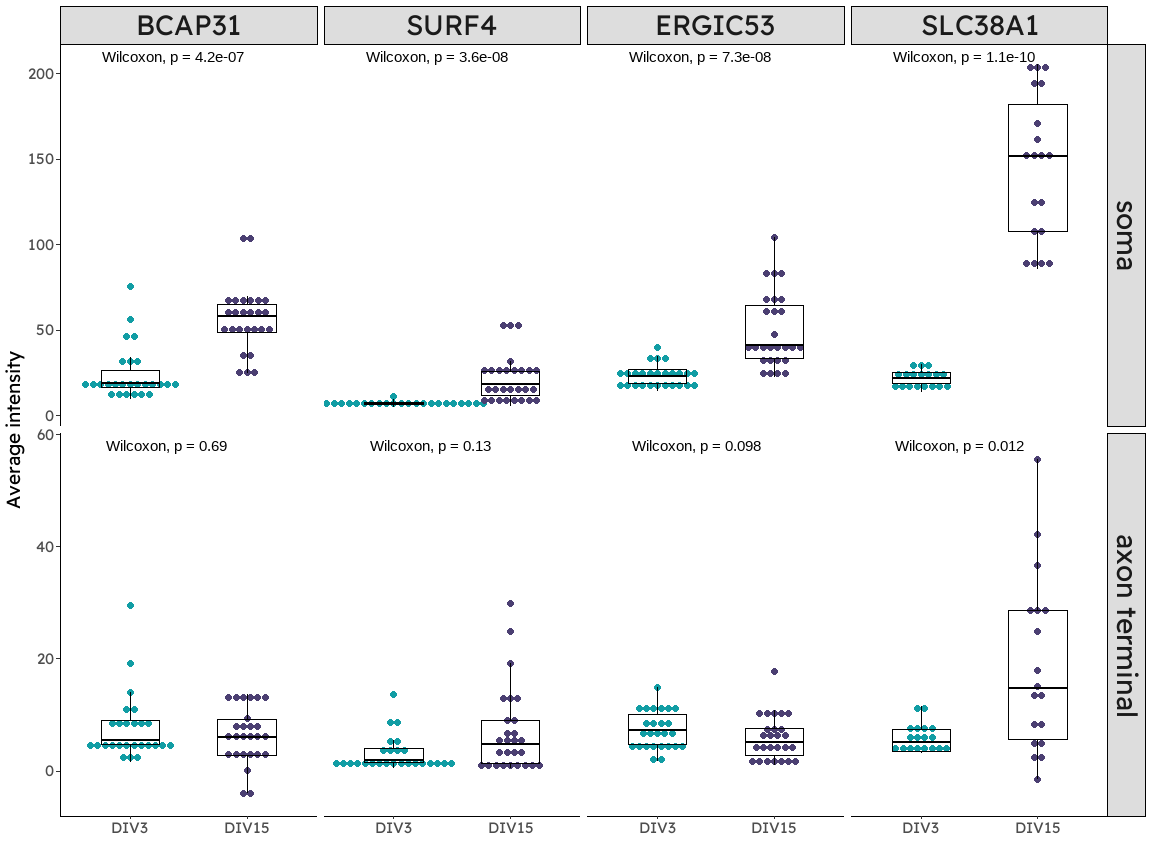
\includegraphics{./figures/full/suppl-dev-grid-1} \caption[Marker intensity in cell bodies and axon terminals of developing cortical neurons]{Fluorescence intensity of various markers in DIV3 vs DIV15 rat cortical neurons, divided into cell body or axon terminal. All \emph{n} = 26 or 27 cells per condition across three batches, except SLC38A1 (\emph{n} = 18 cells, three batches). Wilcoxon rank-sum \emph{p} values are shown at the top of each plot.}\label{fig:suppl-dev-grid}
\end{figure}

The staining was repeated in DIV1 (post-differentiation) i3 neurons, at a stage when they are just beginning to grow axons, to confirm that the axon terminal:cell body ratio was conserved between rodent and human neurons. This showed remarkable consistency between cell types, with the exception of BCAP31, which had a very slightly higher ratio in rat cortical neurons (figure \ref{fig:i3-ratio-plot}).



\begin{figure}
\includegraphics{../figures/full/i3-ratio-plot-1} \caption[Comparison of marker localisation between i3 neurons and rat cortical neurons]{A) Ratio of fluorescence intensity between Cell body and axon terminal in DIV1 i3 vs DIV3 rat cortical neurons. \emph{n} = 17 or 18 i3 neurons per condition across three batches. \emph{n} = 26 or 27 rat cortical neurons per condition across three batches, except SLC38A1 (\emph{n} = 18 cells, three batches). B-E) Representative images of DIV1 i3 neurons stained for each marker. All scale bars are 20 \textmu{}m. Wilcoxon rank-sum \emph{p} values are shown at the top of each plot.}\label{fig:i3-ratio-plot}
\end{figure}

As these results clearly indicate that these secretory pathway markers (with the exception of SURF4) show a relative decline in axon terminals during neuronal maturation, we might expect that treatment with protrudin would increase these concentrations back to early developmental levels to promote axon growth.

\subsection{ER exit site visualisation}\label{er-exit-site-visualisation}

We also tested a tool called ESCargo(FTV) to directly visualise ER exit sites {[}79,167{]}. This encodes a SURF4-dependent synthetic secretory cargo that collects at ER exit sites and can be inducibly released from the ER with the addition of a synthetic ligand. While the aggregates were clearly visible in cell bodies, we also observed them in axons, although they were distributed very sparsely along their length (figure \ref{fig:ESCargo-figure}). In some cases, these were found at axonal swellings or branch points, raising the possibility that these exit sites may concentrate at particular structural features. Our imaging suggests that there are functional ER exit sites in the axons of mature cortical neurons, although further work is required to confirm this result, and to determine whether their size or number is regulated developmentally or with the overexpression of protrudin.

\begin{figure}
\includegraphics{../figures/full/ESCargo-figure-1} \caption[ESCargo localisation in cortical neurons]{A) Cell body of a cell co-expressing EGFP/Emerald with ESCargo(FTV)-Crimson.  Note individual aggregates or small clusters in dendrites, often at branch points.  B) Axon of neuron depicted in A, with two ESCargo(FTV) aggregates circled.  All scale bars are 20 \textmu{}m.}\label{fig:ESCargo-figure}
\end{figure}

\subsection{The role of protrudin in localisation and transport}\label{the-role-of-protrudin-in-localisation-and-transport}

Given the developmental decline in these markers at axon terminals, we were interested to see if protrudin might act by increasing the axonal levels of ER-Golgi pathway components. We repeated the experiment above in DIV15 rat cortical neurons expressing either EGFP or EGFP-tagged protrudin, and measured the fluorescence intensity in the cell body and axon terminals.

\subsubsection{BCAP31}\label{bcap31}

BCAP31 showed high variability between cells, particularly in the soma (figure \ref{fig:BCAP31-plot}, panel H). This may have been a result of signal amplification with a biotinylated secondary antibody, although the smaller range of intensities measured at axon terminals suggests that this may represent natural variation (figure \ref{fig:BCAP31-plot}, panel I). In any case, while protrudin did appear to decrease cell body BCAP31 levels, this did not translate to a change in the axon terminal:cell body ratio (figure \ref{fig:BCAP31-plot}, panel G). Therefore, we do not believe that protrudin substantially changes the distribution of BCAP31 in cortical neurons.

Peculiarly, in many cases BCAP31 signal appeared higher in cells expressing either protrudin or control EGFP, compared to untransfected neighbouring cells (data not shown). It is possible that the levels of this protein are dynamically controlled in response to the cell's overall level of protein synthesis, which may be impacted by exogenous protein expression plasmids. This should be taken into account in any future experiments examining BCAP31 levels or localisation.

\subsubsection{SURF4}\label{surf4}

Unexpectedly, SURF4 \emph{decreased} both in the cell body and axon terminal of cells expressing active protrudin (figure \ref{fig:SURF4-plot}, panels H-I). However, these decreases were well-matched, resulting in no change to the axon terminal:cell body ratio (figure \ref{fig:SURF4-plot}, panel G). Notably, SURF4 was the one marker that did not show any change in axon terminal:cell body ratio with neuronal maturation (figure \ref{fig:dev-changed-full-figure}), and analysis of individual cell compartments showed a developmental \emph{increase} in the soma and a slight but non-significant increase in the axon terminal (figure \ref{fig:suppl-dev-grid}), so the decrease in overall expression level observed with active protrudin may well indicate a change to a more growth-like state. That being said, it is unclear how a decrease in SURF4, as a key ERES-associated protein, would relate to increased growth.

\subsubsection{SLC38A1}\label{slc38a1}

SLC38A1 showed no significant changes with either WT or active protrudin expression, although there was a slight trend towards higher axonal intensity (figure \ref{fig:SLC38A1-plot}). As SLC38A1 levels actually increase significantly in both the cell body and axon terminal with neuronal maturation (figure \ref{fig:suppl-dev-grid}), even as the axon terminal:cell body ratio declines (figure \ref{fig:dev-changed-full-figure}), it would appear that the availability (or lack thereof) of local secretory machinery in mature axons is not a limiting factor for SLC38A1 abundance.

\subsubsection{ERGIC53}\label{ergic53}

In contrast with the other markers, ERGIC53 showed significantly altered localisation with the expression of active, but not wild type, protrudin. This included a significant increase in axon terminal intensity and axon terminal:cell body ratio, on top of a slight increase in soma intensity (figure \ref{fig:ERGIC53-plot}, panels G-I). This strongly suggests that protrudin is playing a role in either the formation of ERGIC compartments, or their transport into the distal axon. As the ERGIC53 axon terminal:cell body ratio typically declines sharply as these cortical neurons mature (figure \ref{fig:dev-changed-full-figure}), this result is consistent with active protrudin restoring axonal ERGIC53 to early developmental levels.



\begin{figure}[H]
\includegraphics{../figures/fullBCAP31-plot-1} \caption[BCAP31 localisation in protrudin-expressing neurons]{A-F) Representative images of BCAP31 in control, WT, and active protrudin-expressing cell bodies (A-C, respectively) and axon terminals (D-F). All scale bars are 20 \textmu{}m, and D-F are 20x20 \textmu{}m. G-I) Quantification of BCAP31 fluorescence intensity. \emph{n} = 18 cells per condition across three independent batches. Kruskal-Wallis \emph{p} values are shown at the top of each plot; significant \emph{p} values from Dunn's post-hoc test with Bonferroni correction for multiple comparisons are shown over brackets.}\label{fig:BCAP31-plot}
\end{figure}



\begin{figure}[H]
\includegraphics{../figures/fullSURF4-plot-1} \caption[SURF4 localisation in protrudin-expressing neurons]{A-F) Representative images of SURF4 in control, WT, and active protrudin-expressing cell bodies (A-C, respectively) and axon terminals (D-F). All scale bars are 20 \textmu{}m, and D-F are 20x20 \textmu{}m. G-I) Quantification of SURF4 fluorescence intensity. \emph{n} = 17 or 18 cells per condition across three independent batches. Kruskal-Wallis \emph{p} values are shown at the top of each plot; significant \emph{p} values from Dunn's post-hoc test with Bonferroni correction for multiple comparisons are shown over brackets.}\label{fig:SURF4-plot}
\end{figure}



\begin{figure}[H]
\includegraphics{../figures/fullSLC38A1-plot-1} \caption[SLC38A1 localisation in protrudin-expressing neurons]{A-F) Representative images of SLC38A1 in control, WT, and active protrudin-expressing cell bodies (A-C, respectively) and axon terminals (D-F). All scale bars are 20 \textmu{}m, and D-F are 20x20 \textmu{}m. G-I) Quantification of SLC38A1 fluorescence intensity. \emph{n} = 15 to 18 cells per condition across three independent batches. Kruskal-Wallis \emph{p} values are shown at the top of each plot.}\label{fig:SLC38A1-plot}
\end{figure}



\begin{figure}[H]
\includegraphics{../figures/fullERGIC53-plot-1} \caption[ERGIC53 localisation in protrudin-expressing neurons]{A-F) Representative images of ERGIC53 in control, WT, and active protrudin-expressing cell bodies (A-C, respectively) and axon terminals (D-F). All scale bars are 20 \textmu{}m, and D-F are 20x20 \textmu{}m. G-I) Quantification of ERGIC53 fluorescence intensity. \emph{n} = 16 or 18 cells per condition across three independent batches. Kruskal-Wallis \emph{p} values are shown at the top of each plot; significant \emph{p} values from Dunn's post-hoc test with Bonferroni correction for multiple comparisons are shown over brackets.}\label{fig:ERGIC53-plot}
\end{figure}

\subsection{Protrudin's effect on Golgi satellites}\label{protrudins-effect-on-golgi-satellites}

Given protrudin's effect on the ERGIC compartment, we were particularly interested in seeing if this also impacted axonal Golgi satellites. As these are highly dynamic organelles, we decided to look at Golgi satellite transport in the presence of protrudin. Using rat cortical neurons, we co-expressed mCherry-tagged protrudin constructs with ST3GAL5-EGFP, a marker of Golgi satellites {[}83{]}. We then imaged the axons in three-minute segments on a spinning disc confocal microscope, as described previously for LAMP1 and RAB7 in section \ref{lyso-LE}.

This revealed no change in overall number of Golgi satellites in the distal axon, but a significant slowing of anterograde transport in cells expressing active protrudin (figure \ref{fig:ST3GAL5-full-figure}, panels B, D). This mirrors the effect of axonal protrudin on LAMP1 transport, and is discussed further below in section \ref{GS-discussion}.



\begin{figure}
\includegraphics{../figures/full/ST3GAL5-full-figure-1} \caption[Protrudin effect on Golgi satellite (ST3GAL5) transport in the distal axon]{A) Representative axon image and kymographs showing ST3GAL5 transport in the distal axon of cortical neurons expressing either mCherry (control) or mCherry-tagged protrudin constructs. All scale bars are 20 \textmu{}m. B) Total number of ST3GAL5-labelled organelles in each cell imaged. C) Average run length (per cell) of moving Golgi satellites D) Average Golgi satellite velocity (per cell). \emph{n} = 22 or 24 cells per condition across three independent batches. Kruskal-Wallis \emph{p} values are shown at the top of each plot; significant \emph{p} values from Dunn's post-hoc test with Bonferroni correction for multiple comparisons are shown over brackets.}\label{fig:ST3GAL5-full-figure}
\end{figure}

Following live imaging, these cells were fixed, and imaged at higher exposure on a confocal microscope to more clearly visualise Golgi satellites in the axon. We measured both the number of puncta as well as point intensity of each, as a proxy for size. This confirmed that protrudin overexpression did not affect the overall number of Golgi satellites in the distal axon, nor did it appear to affect the size of these organelles (figure \ref{fig:GS-puncta-full-figure}).



\begin{figure}
\includegraphics{../figures/full/GS-puncta-full-figure-1} \caption[Protrudin effect on Golgi satellite abundance and size in the distal axon]{A) Representative axon image showing ST3GAL5 puncta. Scale bar is 20 \textmu{}m. B) Zoomed-in view of the 20 x 20 \textmu{}m box in panel A. Counted puncta are indicated by arrows. C) Number of puncta per \textmu{}m of axon imaged. D)Point fluorescence intensity of each ST3GAL5 puncta counted. \emph{n} = 18 cells per condition across three independent batches. Kruskal-Wallis \emph{p} values are shown at the top of each plot.}\label{fig:GS-puncta-full-figure}
\end{figure}

We then conducted a scratch assay to determine the localisation of Golgi satellites in the growth cones of mature neurons and examine whether protrudin might have an effect on axonal Golgi satellites in response to injury. Cortical neurons cultured on glass coverslips were scratched with a sterile needle, then incubated for 18-20 hours before fixing. Axons growing into the scratched region were imaged on a confocal microscope. While this method cuts axons, dendrites, and cell bodies indiscriminately, and does not directly measure regeneration, it is useful for isolating growth cones in mature (DIV15) cortical neurons.

This revealed a strong concentration of ST3GAL5 at the base of each growth cone, with slightly weaker signal extending further distally (figure \ref{fig:scratch-assay-full}, panels A-C). Where ST3GAL5 was co-expressed with protrudin, it is apparent that the Golgi satellite signal reaches further into the growth cone than the ER (figure \ref{fig:scratch-assay-full}, panels E-F). This suggests that there are distinct ER and Golgi compartments in the growth cone, with secretory machinery oriented towards the direction of growth. The images also suggest that there might be an accumulation of ST3GAL5 immediately proximal to the growth cone in protrudin-expressing neurons (figure \ref{fig:scratch-assay-full}, panels E-F), although further work is required to confirm and quantify this result.

\begin{figure}
\includegraphics{../figures/full/scratch-assay-full-1} \caption[Scratch assay of neurons co-expressing protrudin and ST3GAL5]{Representative images of growth cones on DIV15 cortical neurons after scratch.  Neurons are co-expressing either mCherry (A) or mCherry-protrudin (B-C) with ST3GAL5-EGFP.  Scale bars are 20 \textmu{}m.  D-F) 20x20 \textmu{}m images highlighting the growth cone details shown in A-C.  Arrows indicate large Golgi satellites, as well as the distal edge of protrudin localisation.  Note how the ST3GAL5 signal extends beyond protrudin in these growth cones.}\label{fig:scratch-assay-full}
\end{figure}

\section{Discussion}\label{discussion-1}

\subsection{Protrudin's effects on the local secretory pathway}\label{protrudins-effects-on-the-local-secretory-pathway}

\subsubsection{Increased ERGIC53 in axon terminals}\label{increased-ergic53-in-axon-terminals}

These results provide an insight into how protrudin might regulate local secretory pathways in the axon. While protrudin does not appear to change the distribution of primarily ERES-associated proteins, such as BCAP31 and SURF4, active protrudin does significantly increase the relative level of ERGIC53 in axon terminals.

As the ERGIC is a distinct compartment from the ER, this suggests a secretory role for protrudin beyond its effects on the axonal ER. It is not yet clear if this represents an increased formation of ERGIC from ERES-derived vesicles in the axon, or increased transport of these structures from elsewhere in the cell. Further work will use a GFP-tagged ERGIC53 construct to examine whether the ERGIC compartments are transported axonally, and whether this transport is affected by protrudin. In any case, the increase in ERGIC observed with protrudin expression should be beneficial to local protein production and secretion, and providing the machinery for efficient cargo sorting might allow for increased growth after axonal injury.

\subsubsection{Slower Golgi satellite transport}\label{GS-discussion}

This is further supported by our finding that active protrudin affects Golgi satellite transport in the distal axon. Unexpectedly, we found slower transport of Golgi satellites in the distal axon, particularly in the anterograde direction, despite unchanged run length or overall number of organelles. Further experiments are required to identify a mechanism for this change, although it could represent a sustained interaction with another organelle during transport, potentially ERGIC or a related compartment.

If this interaction is between Golgi satellites and lysosomes, this could explain the slight slowing of lysosomes observed previously with active protrudin (figure \ref{fig:LAMP1-full-figure}, panel D). Lie et al.~identified `post-Golgi carriers' as the source of degradative enzymes for maturing axonal lysosomes, which could indicate just such an interaction {[}166{]}. However, the marker they used for the carriers (\emph{trans}-Golgi marker TGN38) is not commonly found in Golgi satellites, so this might represent a distinct organelle {[}83{]}.

The marker we used for Golgi satellites --- ST3GAL5 --- gives us some hints as to how Golgi satellite interactions in the axon might relate to growth and regenerative function. ST3GAL5 is a lipid sialylation enzyme, and synthesises a ganglioside (a type of modified glycolipid) known as GM3. ST3GAL5 mutations in humans are linked to severe neurological syndromes, indicating a key role in normal CNS function. Furthermore, other gangliosides produced downstream of GM3 have been shown to increase regeneration in several different models of axon injury, indicating another mechanism through which protrudin might promote regeneration {[}177,178{]}

That being said, it remains to be seen how protrudin's effect on Golgi satellite \emph{transport} translates into an effect on Golgi satellite \emph{function} in the axon. It could reasonably be argued that slower transport would decrease the number of inter-organelle contacts made by each satellite, thereby decreasing their effect (e.g.~in the case of lysosomal enzyme delivery, as suggested by Lie et al.) {[}166{]}. Conversely, it would not be unreasonable to suggest that slower transport might indicate more prolonged interactions, for example with ERGIC, that could increase their ability to receive secretory cargo and allow enzymes such as ST3GAL5 to carry out their functions. Further work is required to better understand which organelles interact with Golgi satellites in the axon, and how these interactions are influenced by protrudin.

\subsubsection{Golgi satellites in the growth cone}\label{golgi-satellites-in-the-growth-cone}

Our scratch assay also revealed a concentration of Golgi satellites in the growth cones of mature neurons. While these results are only preliminary, they suggest a key role for Golgi satellites in axonal growth. The additional observation of an additional ST3GAL5 accumulation proximal to the growth cone in protrudin-expressing neurons is also interesting --- while it is not immediately clear what this represents, it might indicate a further increase in secretory machinery in the distal axon, which could promote regeneration.

These findings indicate that protrudin overexpression, particularly active protrudin, has a significant impact on the local secretory machinery present in the axon, which may play a role in mediating protrudin's neuroprotective and regenerative effects. Additionally, these results may account for the finding that active protrudin has a stronger regenerative effect than WT protrudin, but that the two constructs do not significantly differ in measures of RAB11 or integrin transport {[}62{]}.

\chapter*{Discussion}\label{DISCUSSION}
\addcontentsline{toc}{chapter}{Discussion}

\markboth{DISCUSSION}{}
\setcounter{chapter}{4}
\setcounter{section}{0}
\setcounter{figure}{0}

\section{Results}\label{results-3}

\subsection{Protrudin's role in axonal transport}\label{protrudins-role-in-axonal-transport}

Perhaps the most surprising finding of this project has been that protrudin overexpression has little if any effect on lysosome or late endosome transport in cortical neurons. Initially, this seems to conflict with previous work in other cell types, which suggest that protrudin has a strong effect on late endosome transport and positioning, {[}56,101{]}. However, this is in fact consistent with the mechanism proposed in those studies, which identifies FYCO1 as the actual adaptor between late endosomes and kinesin. As numerous RNAseq data sets show that there is extremely little FYCO1 in CNS neurons (figure \ref{fig:FYCO1-RNAseq-full-figure}), it seems likely that this mechanism is not active in these neurons. Instead, anterograde lysosome/late endosome transport in axons is probably mediated primarily by the BORC/ARL8B/SKIP mechanism, as suggested by Farias et al. {[}112{]}.

This apparent cell-type variability in protrudin function has important implications for its development as a regenerative gene therapy. Further work will be required to characterise the effects of protrudin overexpression on different cell types and tissues, and to ensure that therapeutic vectors target protrudin expression to the correct cellular population.

In addition, this finding raises interesting questions about the role of FYCO1 in regeneration. As FYCO1 appears to facilitate protrudin's role in cellular outgrowth, but is largely absent from mature CNS neurons, it is possible that FYCO1 expression is correlated with the intrinsic regenerative capacity of different cell types. Investigating this further might shed more light on why most CNS neurons are such poor regenerators, and identify novel targets to promote regeneration.

The effect of active protrudin on Golgi satellite transport (figure \ref{fig:ST3GAL5-full-figure}), in contrast with late endosomes (in particular those marked by RAB7, as shown in figure \ref{fig:RAB7-full-figure}), shows that protrudin has specific and distinct effects on different organelles in the axon. This is further confirmed by Petrova et al., which showed that both wild type and active protrudin increased the number of RAB11 recycling endosomes in the distal axon, an effect not seen with any of the transport markers used in this thesis {[}62{]}. Based on these results, we can confidently say that protrudin does not indiscriminately increase axonal transport or localisation, but rather specifically mediates the organisation and behaviour of particular organelles through distinct mechanisms.

\subsection{Protrudin's role in local translation}\label{protrudins-role-in-local-translation}

Given its effect on ERGIC localisation (figure \ref{fig:ERGIC53-plot}) and the dynamics of Golgi satellite transport (figure \ref{fig:ST3GAL5-full-figure}), it appears that protrudin overexpression --- particularly active protrudin --- has a significant effect on the local secretory machinery in axons. Considering the importance of local translation on axon function and growth, as discussed previously, it is easy to see how this might contribute to both protrudin's neuroprotective and regenerative effects. Additionally, recent work has indicated a direct link between the level of local translation in axons and their regenerative capacity, supporting the idea that protrudin could act by coordinating machinery for local protein synthesis and processing {[}154{]}.

This is worth considering in the context of the previous finding that protrudin increases the amount of RAB11 recycling endosomes in the distal axon {[}62{]}. Bowen et al.~showed that recycling endosomes can play a role in the secretion of locally translated proteins in dendrites, either through Golgi satellites or entirely bypassing Golgi-related compartments {[}143{]}. Therefore, it is possible that these endosomes also comprise part of the secretory machinery in axons, in addition to ERGIC and Golgi satellites.

Further work will be required to identify the molecular mechanisms at play in this process, and whether it is a result of direct protrudin interactions or is downstream of other cellular effects. This may well vary for each component of the secretory pathway --- for example, protrudin can bind to RAB11 directly to facilitate recycling endosome transport, but no such interactions have yet been identified for ERGIC or Golgi satellites. However, the presence of numerous Golgi-related proteins in protrudin interactomes (figure \ref{fig:proteomics-full-figure}) strongly suggests a direct involvement in ER-Golgi interactions.

\section{Future directions}\label{future-directions}

While this project has provided some answers to how protrudin can promote survival and regeneration, it also raises new questions which should be addressed in future studies. In addition to the follow-up experiments mentioned above, several other systems should be investigated in the context of protrudin overexpression to understand their impact on its neuroprotective and regenerative effects.

\subsection{Autophagy}\label{autophagy}

Protrudin's effects on LC3 localisation, both in HeLa cells and cortical neurons (figure \ref{fig:LC3-full-figure}), suggest an active role in regulating autophagy. The preliminary results demonstrated in this project suggest that protrudin may increase autophagy or autophagosome biogenesis. However, Hong et al.~actually found the opposite --- protrudin \emph{depletion} promoted autophagy initiation in cultured epithelial cells {[}101{]}.

It is very likely that this effect varies by cell type, similar to the effect on lysosomal transport, and for the same reason --- FYCO1 acts as an adaptor for autophagosome transport, and is involved in autophagosome maturation {[}82,179{]}. However, there are other potential mechanisms through which protrudin could affect neuronal autophagy in the absence of FYCO1, as both ER contact sites and RAB11 endosomes have been implicated in early autophagosome formation {[}180,181{]}

With this in mind, it would be worthwhile to examine further what effect protrudin overexpression has on autophagy, particularly in CNS neurons. Given the abundance of literature linking autophagy to neuronal survival {[}reviewed in 149{]}, this may well represent another pathway through which protrudin acts, particularly in a neuroprotective role.

\subsection{Lipids}\label{discussion-lipids}

Numerous results throughout this thesis suggest a link between protrudin and lipid metabolism. The gene ontology analysis in section \ref{GO-analysis} highlighted a number of protrudin interactions with genes involved in lipid metabolism. The unusual localisation of BODIPY C\textsubscript{5} ceramide in HeLa cells expressing protrudin also supports the idea of an effect on lipid pathways in the cell (figure \ref{fig:ceramide-full-figure}). Furthermore, the enzyme ST3GAL5, used in this thesis as a marker for Golgi satellites, is an enzyme important for the production of gangliosides, glycolipids that form a key component of neuronal cell membranes and are important for axonal growth and maintenance {[}reviewed in 182{]}. Given protrudin's effect on the transport of these organelles, this could suggest a change to how lipids are metabolised and processed in the axon. Ewan et al.~identified changes in lipid metabolism as a key factor distinguishing PNS from CNS axon regeneration, suggesting that protrudin could potentially promote regeneration through these pathways {[}45{]}.

In a collaborative project with the Williams lab at the Karolinska Institutet, mice were injected intravitreally with AAV2 encoding the CAG protrudin constructs used in this thesis. Lipid mass spectroscopy of these mice's optic nerves showed that either WT or active protrudin expression decreased the level of ceramides while increasing hexosylceramides, pointing to an effect on sphingolipid synthesis pathways (data not shown). Further work is ongoing in this area to understand how protrudin overexpression influences lipid pathways in the cell, and what effect this has on neuronal survival and regeneration.

\subsection{Mitochondria}\label{mitochondria-1}

Previous work has suggested that protrudin may play a role at ER-mitochondrial contact sites {[}65,183{]}, although it is not yet clear what effects this may have on the cell. Preliminary EM data from another collaboration with the Williams lab show some unusually long mitochondria in the optic nerves of mice expressing active protrudin, which were not observed with a GFP control (data not shown). Work is ongoing to confirm this result and examine potential mechanisms.

\section{Implications for glaucoma therapy}\label{implications-for-glaucoma-therapy}

Given that the initial aim of this project was to develop protrudin into a gene therapy for glaucoma, it is worth considering these findings in that context. While we were unable to perform \emph{in vivo} experiments during this project, the results presented in this thesis still have important implications for future work in this area.

As discussed above, the lack of any apparent effect of protrudin expression on axonal lysosome and late endosome transport, due to the absence of FYCO1, indicates that protrudin is likely to have very different effects on different cell types. While initial \emph{in vivo} experiments with protrudin have shown very positive results, with significantly improved retinal ganglion cell survival and regeneration after an optic nerve crush, care should be taken to look out for any expression outside of this target cell population, and to characterise the effect of protrudin overexpression in glial and epithelial cell lines {[}62{]}.

Furthermore, the results presented in chapters 2 and 3 of this thesis identify a new cellular system --- the local secretory pathway --- through which protrudin might act to promote survival and regeneration in CNS neurons. Other components of this pathway, particularly any that might regulate localisation or inter-organelle interactions, should therefore be examined for potential neuroprotective and regenerative benefits. While it may be possible to identify entirely new gene therapy candidates in this way, it might also be possible to identify proteins that can act synergistically with protrudin for improved therapeutic effects.

\section{Conclusion --- A unifying site of action}\label{conclusion-a-unifying-site-of-action}

The results of this project, taken in combination with previous work, suggest that protrudin is coordinating an `axon trafficking centre', increasing ER tubules, ERGIC, and recycling endosomes --- all key components of the local secretory pathway --- in the distal axon. Through the actions of the virtuous cycle, this arrangement of organelles can promote integrin delivery, facilitate local protein translation and processing, and encourage growth-promoting signalling cascades to increase survival and axonal regeneration.

Whether this coordination occurs through direct interactions or downstream of other cellular effects is unclear, but it seems likely that this is a contributing factor to protrudin's effectiveness as a CNS therapy. Future work in this area should be focused on the structure and nature of interactions between pathway components (ER, ERGIC, Golgi satellites, and endosomes), how they are recruited to sites of axonal injury or degeneration, and whether they are directly associated with regenerative ability.

\chapter*{Appendix}\label{APPENDIX}
\addcontentsline{toc}{chapter}{Appendix}

\markboth{APPENDIX}{}
\setcounter{chapter}{5}
\setcounter{section}{0}
\setcounter{figure}{0}

\section{Supplementary Figures}\label{SUPPLEMENT}

\begin{figure}
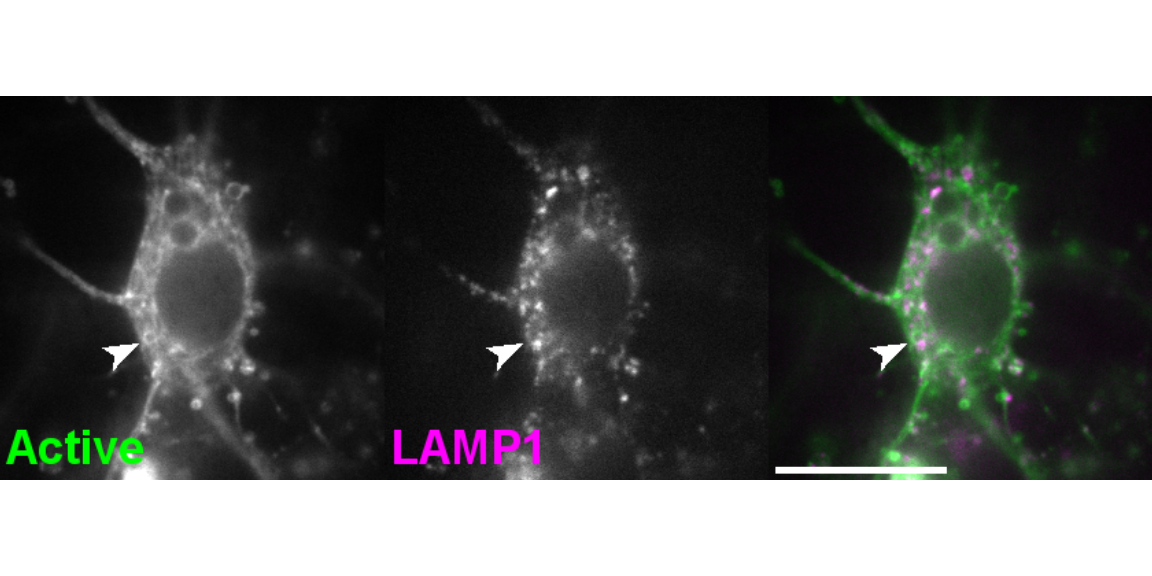
\includegraphics{./figures/full/suppl-ring-1} \caption[Supplementary figure; Example image of a ring-like structure in a neuron]{Example image of a ring-like structure in a neuron co-expressing active protrudin and LAMP1.  Note that LAMP1 does not label the structure directly, but appears to label an adjacent organelle.  The larger rings towards the top of the cell have a much dimmer protrudin 'ring', and appear to be vacuoles.  Scale bar is 20 \textmu{}m.}\label{fig:suppl-ring}
\end{figure}



\begin{figure}
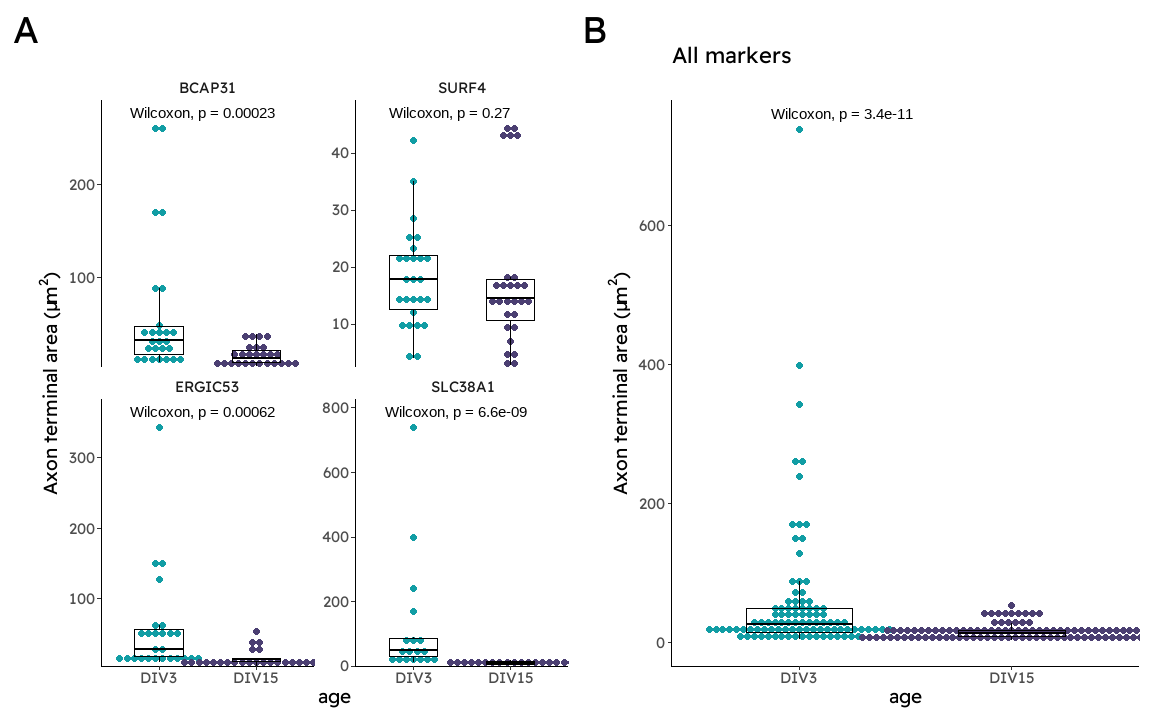
\includegraphics{./figures/full/suppl-gc-area-1} \caption[Supplementary figure; axon terminal area in developing cortical neurons]{Axon terminal area of DIV3 vs DIV15 rat cortical neurons, A) for each marker and B) pooled together. All show a significant decrease in axon terminal area during development, with the exception of SURF4. Given the substantially smaller measurements in DIV3 neurons stained for SURF4 compared to other markers, this suggests that SURF4 is confined to the central region of the developing growth cone. All \emph{n} = 26 or 27 cells per condition across three batches, except SLC38A1 (\emph{n} = 18 cells, three batches). Wilcoxon rank-sum \emph{p} values are shown at the top of each plot.}\label{fig:suppl-gc-area}
\end{figure}

\section{Plasmid Maps}\label{plasmid-maps}

\includegraphics{../figures/plasmid-maps-1-1.png}

\includegraphics{../figures/plasmid-maps-2-1.png}

\includegraphics{../figures/plasmid-maps-3-1.png}

\section{Code}\label{CODE}

In this section, I have included many of the ImageJ macros (written in the ImageJ Macro language) and R scripts that I wrote to simplify collecting and analysing data over the course of this project. All are freely available to use and modify; if you use them extensively for your own work, please cite this thesis. You might find the occasional `TODO' in with the more descriptive comments; I have left these in place as suggestions for future improvements.

\subsection{ImageJ Macros}\label{imagej-macros}

\subsubsection{Axon puncta counter}\label{axon-puncta-counter}

Used to streamline the process of manually counting axonal puncta, as in \ref{fig:GS-puncta-full-figure}. Displays the first image from each timelapse stack in a directory, plots a low-opacity trace of the axon to be analysed, and selects the multipoint tool for the user. Results are saved to a CSV file at the end of the batch. Requires a folder of STK or TIF image stacks and RGN or ROI files with matching names.

\begin{Shaded}
\begin{Highlighting}[]
\NormalTok{setBatchMode}\OperatorTok{(}\KeywordTok{false}\OperatorTok{);}\CommentTok{//interactive}

\NormalTok{function main}\OperatorTok{(}\NormalTok{i}\OperatorTok{)\{}
    \CommentTok{//{-}{-}{-}duplicate fist frame of stack, close original, and make all changes on duplicate{-}{-}{-}}
\NormalTok{    rename}\OperatorTok{(}\StringTok{"orig"}\OperatorTok{);}
\NormalTok{    run}\OperatorTok{(}\StringTok{"Duplicate..."}\OperatorTok{,} \StringTok{"title=["}\OperatorTok{+}\NormalTok{getInfo}\OperatorTok{(}\StringTok{"image.filename"}\OperatorTok{)+}\StringTok{"\_duplicate] duplicate range=1{-}1"}\OperatorTok{);}
\NormalTok{    close}\OperatorTok{(}\StringTok{"orig"}\OperatorTok{);}
\NormalTok{    rename}\OperatorTok{(}\StringTok{"duplicate"}\OperatorTok{);}\CommentTok{//for closing later and to obscure file name for blind analysis}

    \CommentTok{//{-}{-}{-}load and measure ROI, draw transparent over image{-}{-}{-}}
    \CommentTok{//loaded in batch runner}
    \CommentTok{//run("ROI Manager...");}
\NormalTok{    roiManager}\OperatorTok{(}\StringTok{"select"}\OperatorTok{,} \DecValTok{0}\OperatorTok{);}
\NormalTok{    run}\OperatorTok{(}\StringTok{"Measure"}\OperatorTok{);}
\NormalTok{    ROI\_length }\OperatorTok{=}\NormalTok{ getResult}\OperatorTok{(}\StringTok{"Length"}\OperatorTok{,} \DecValTok{0}\OperatorTok{);}
\NormalTok{    roiManager}\OperatorTok{(}\StringTok{"Show All"}\OperatorTok{);}

    \CommentTok{//{-}{-}{-}multipoint tool, dialog to confirm{-}{-}{-}}
\NormalTok{    close}\OperatorTok{(}\StringTok{"Results"}\OperatorTok{);}
\NormalTok{    setTool}\OperatorTok{(}\StringTok{"multipoint"}\OperatorTok{);}
        
\NormalTok{    Dialog}\OperatorTok{.}\NormalTok{createNonBlocking}\OperatorTok{(}\StringTok{"Confirm points"}\OperatorTok{);}
\NormalTok{    Dialog}\OperatorTok{.}\NormalTok{addMessage}\OperatorTok{(}\StringTok{"Click \textquotesingle{}OK\textquotesingle{} to confirm points."}\OperatorTok{);}
    \CommentTok{//}\AlertTok{TODO}\CommentTok{ {-} option to skip/exclude?}
\NormalTok{    Dialog}\OperatorTok{.}\NormalTok{show}\OperatorTok{();}
    
\NormalTok{    run}\OperatorTok{(}\StringTok{"Measure"}\OperatorTok{);}\CommentTok{//will count 1 if no points added {-} defaults to last active ROI}
    \CommentTok{//check if any points have been added}
    \ControlFlowTok{if}\OperatorTok{(}\NormalTok{selectionType}\OperatorTok{()} \OperatorTok{==} \OperatorTok{{-}}\DecValTok{1}\OperatorTok{)\{}\CommentTok{//no points added}
\NormalTok{        count }\OperatorTok{=} \DecValTok{0}\OperatorTok{;}
    \OperatorTok{\}}
    \ControlFlowTok{else}\OperatorTok{\{}
\NormalTok{        count }\OperatorTok{=}\NormalTok{ getValue}\OperatorTok{(}\StringTok{"results.count"}\OperatorTok{);}
    \OperatorTok{\}}
        
    \CommentTok{//{-}{-}{-}write filename, point count, ROI length to Table{-}{-}{-}}
\NormalTok{    selectWindow}\OperatorTok{(}\StringTok{"Puncta counts"}\OperatorTok{);}\CommentTok{//}\AlertTok{TODO}\CommentTok{ pass as parameter}
\NormalTok{    Table}\OperatorTok{.}\NormalTok{set}\OperatorTok{(}\StringTok{"File"}\OperatorTok{,}\NormalTok{ i}\OperatorTok{,}\NormalTok{ stacks}\OperatorTok{[}\NormalTok{i}\OperatorTok{]);}
\NormalTok{    Table}\OperatorTok{.}\NormalTok{set}\OperatorTok{(}\StringTok{"ROI\_length"}\OperatorTok{,}\NormalTok{ i}\OperatorTok{,}\NormalTok{ ROI\_length}\OperatorTok{);}
\NormalTok{    Table}\OperatorTok{.}\NormalTok{set}\OperatorTok{(}\StringTok{"Count"}\OperatorTok{,}\NormalTok{ i}\OperatorTok{,}\NormalTok{ count}\OperatorTok{);}
\NormalTok{    Table}\OperatorTok{.}\NormalTok{update}\OperatorTok{();}
    
    \CommentTok{//{-}{-}{-}close image and extra windows}
\NormalTok{    close}\OperatorTok{(}\StringTok{"duplicate"}\OperatorTok{);}\CommentTok{//not working}
    \CommentTok{//tables handled in batch runner}
\OperatorTok{\}}

\CommentTok{//{-}{-}{-}batch runner{-}{-}{-}}
\NormalTok{dir }\OperatorTok{=}\NormalTok{ getDirectory}\OperatorTok{(}\StringTok{"Choose a Directory"}\OperatorTok{);}
\NormalTok{File}\OperatorTok{.}\NormalTok{makeDirectory}\OperatorTok{(}\NormalTok{dir }\OperatorTok{+} \StringTok{"puncta\_counts"}\OperatorTok{);}

\NormalTok{Dialog}\OperatorTok{.}\NormalTok{create}\OperatorTok{(}\StringTok{"Options"}\OperatorTok{);}
\NormalTok{Dialog}\OperatorTok{.}\NormalTok{addChoice}\OperatorTok{(}\StringTok{"File extension"}\OperatorTok{,}\NormalTok{ newArray}\OperatorTok{(}\StringTok{"stk"}\OperatorTok{,} \StringTok{"tif"}\OperatorTok{),} \StringTok{"stk"}\OperatorTok{);}
\NormalTok{Dialog}\OperatorTok{.}\NormalTok{show}\OperatorTok{();}
\NormalTok{ext }\OperatorTok{=}\NormalTok{ Dialog}\OperatorTok{.}\NormalTok{getChoice}\OperatorTok{();}

\NormalTok{files }\OperatorTok{=}\NormalTok{ getFileList}\OperatorTok{(}\NormalTok{dir}\OperatorTok{);}
\CommentTok{//exclude directories}
\NormalTok{temp\_stacks }\OperatorTok{=}\NormalTok{ newArray}\OperatorTok{(}\DecValTok{0}\OperatorTok{);}
\NormalTok{temp\_ROIs }\OperatorTok{=}\NormalTok{ newArray}\OperatorTok{(}\DecValTok{0}\OperatorTok{);}
\ControlFlowTok{for}\OperatorTok{(}\NormalTok{i }\OperatorTok{=} \DecValTok{0}\OperatorTok{;}\NormalTok{ i }\OperatorTok{\textless{}}\NormalTok{ files}\OperatorTok{.}\NormalTok{length}\OperatorTok{;}\NormalTok{ i}\OperatorTok{++)\{}
    \ControlFlowTok{if}\OperatorTok{(!}\NormalTok{endsWith}\OperatorTok{(}\NormalTok{files}\OperatorTok{[}\NormalTok{i}\OperatorTok{],} \StringTok{"/"}\OperatorTok{)\&\&!}\NormalTok{endsWith}\OperatorTok{(}\NormalTok{toLowerCase}\OperatorTok{(}\NormalTok{files}\OperatorTok{[}\NormalTok{i}\OperatorTok{]),} \StringTok{".ini"}\OperatorTok{))\{}
        \ControlFlowTok{if}\OperatorTok{(}\NormalTok{endsWith}\OperatorTok{(}\NormalTok{toLowerCase}\OperatorTok{(}\NormalTok{files}\OperatorTok{[}\NormalTok{i}\OperatorTok{]),} \StringTok{".stk"}\OperatorTok{)||}\NormalTok{endsWith}\OperatorTok{(}\NormalTok{toLowerCase}\OperatorTok{(}\NormalTok{files}\OperatorTok{[}\NormalTok{i}\OperatorTok{]),} \StringTok{".tif"}\OperatorTok{))\{}
\NormalTok{            temp\_stacks }\OperatorTok{=}\NormalTok{ Array}\OperatorTok{.}\NormalTok{concat}\OperatorTok{(}\NormalTok{temp\_stacks}\OperatorTok{,}\NormalTok{files}\OperatorTok{[}\NormalTok{i}\OperatorTok{]);}
        \OperatorTok{\}}
        \CommentTok{//if(endsWith(toLowerCase(files[i]), ".roi"))\{}
        \CommentTok{//  temp\_ROIs = Array.concat(temp\_ROIs,files[i]);}
        \CommentTok{//\}}
    \OperatorTok{\}}
\OperatorTok{\}}
\NormalTok{stacks }\OperatorTok{=}\NormalTok{ temp\_stacks}\OperatorTok{;}
\CommentTok{//rois = temp\_ROIs//unnecessary?}
\NormalTok{shuffle}\OperatorTok{(}\NormalTok{stacks}\OperatorTok{);}\CommentTok{//random order to reduce bias}

\CommentTok{//create custom results table}
\NormalTok{Table}\OperatorTok{.}\NormalTok{create}\OperatorTok{(}\StringTok{"Puncta counts"}\OperatorTok{);}
\NormalTok{Table}\OperatorTok{.}\NormalTok{setColumn}\OperatorTok{(}\StringTok{"File"}\OperatorTok{,}\NormalTok{ newArray}\OperatorTok{(}\DecValTok{0}\OperatorTok{));}
\NormalTok{Table}\OperatorTok{.}\NormalTok{setColumn}\OperatorTok{(}\StringTok{"ROI\_length"}\OperatorTok{,}\NormalTok{ newArray}\OperatorTok{(}\DecValTok{0}\OperatorTok{));}
\NormalTok{Table}\OperatorTok{.}\NormalTok{setColumn}\OperatorTok{(}\StringTok{"Count"}\OperatorTok{,}\NormalTok{ newArray}\OperatorTok{(}\DecValTok{0}\OperatorTok{));}
    
\ControlFlowTok{for}\OperatorTok{(}\NormalTok{i }\OperatorTok{=} \DecValTok{0}\OperatorTok{;}\NormalTok{ i }\OperatorTok{\textless{}}\NormalTok{ stacks}\OperatorTok{.}\NormalTok{length}\OperatorTok{;}\NormalTok{ i}\OperatorTok{++)\{}
\NormalTok{    open}\OperatorTok{(}\NormalTok{dir }\OperatorTok{+}\NormalTok{ stacks}\OperatorTok{[}\NormalTok{i}\OperatorTok{]);}
    
    \CommentTok{//find and open matching ROI}
    \ControlFlowTok{if}\OperatorTok{(}\NormalTok{ext }\OperatorTok{==} \StringTok{"stk"}\OperatorTok{)} \OperatorTok{\{}\NormalTok{roi\_name }\OperatorTok{=}\NormalTok{ replace}\OperatorTok{(}\NormalTok{replace}\OperatorTok{(}\NormalTok{stacks}\OperatorTok{[}\NormalTok{i}\OperatorTok{],}\NormalTok{ ext}\OperatorTok{,} \StringTok{"roi"}\OperatorTok{),} \StringTok{"\_W}\SpecialCharTok{\textbackslash{}\textbackslash{}}\StringTok{d+\_T"}\OperatorTok{,} \StringTok{""}\OperatorTok{);\}}
    \ControlFlowTok{else} \OperatorTok{\{}\NormalTok{roi\_name }\OperatorTok{=}\NormalTok{ replace}\OperatorTok{(}\NormalTok{replace}\OperatorTok{(}\NormalTok{stacks}\OperatorTok{[}\NormalTok{i}\OperatorTok{],}\NormalTok{ ext}\OperatorTok{,} \StringTok{"roi"}\OperatorTok{),} \StringTok{"\_ch}\SpecialCharTok{\textbackslash{}\textbackslash{}}\StringTok{d+.*(?=}\SpecialCharTok{\textbackslash{}\textbackslash{}}\StringTok{.roi$)"}\OperatorTok{,} \StringTok{""}\OperatorTok{);\}}

\NormalTok{    roiManager}\OperatorTok{(}\StringTok{"open"}\OperatorTok{,}\NormalTok{ dir }\OperatorTok{+}\NormalTok{ roi\_name}\OperatorTok{);}
\NormalTok{    roiManager}\OperatorTok{(}\StringTok{"Select"}\OperatorTok{,} \DecValTok{0}\OperatorTok{);}
\NormalTok{    roiManager}\OperatorTok{(}\StringTok{"Rename"}\OperatorTok{,} \StringTok{"axon"}\OperatorTok{);}\CommentTok{//obscure name for impartiality while tracing}

\NormalTok{    main}\OperatorTok{(}\NormalTok{i}\OperatorTok{);}
    \CommentTok{//Close results, images, etc.//close("*");}
\NormalTok{    saveAs}\OperatorTok{(}\StringTok{"Results"}\OperatorTok{,}\NormalTok{ dir }\OperatorTok{+} \StringTok{"puncta\_counts/"} \OperatorTok{+}\NormalTok{ stacks}\OperatorTok{[}\NormalTok{i}\OperatorTok{]} \OperatorTok{+} \StringTok{"\_puncta.csv"}\OperatorTok{);}
\NormalTok{    roiManager}\OperatorTok{(}\StringTok{"reset"}\OperatorTok{);}    
\NormalTok{    run}\OperatorTok{(}\StringTok{"Clear Results"}\OperatorTok{);}
\OperatorTok{\}}

\CommentTok{//save table}
\NormalTok{selectWindow}\OperatorTok{(}\StringTok{"Puncta counts"}\OperatorTok{);}
\NormalTok{Table}\OperatorTok{.}\NormalTok{save}\OperatorTok{(}\NormalTok{dir }\OperatorTok{+} \StringTok{"puncta\_counts/counts.csv"}\OperatorTok{);}

\CommentTok{//{-}{-}{-}{-}{-}{-}{-}{-}{-}{-}{-}{-}{-}{-}{-}{-}{-}{-}{-}{-}{-}{-}{-}{-}{-}{-}{-}{-}{-}{-}{-}}
\CommentTok{//Fisher Yates shuffle, from ImageJ example macro RandomizeArray.txt}
\NormalTok{function shuffle}\OperatorTok{(}\NormalTok{array}\OperatorTok{)} \OperatorTok{\{}
\NormalTok{   n }\OperatorTok{=}\NormalTok{ array}\OperatorTok{.}\NormalTok{length}\OperatorTok{;}  \CommentTok{// The number of items left to shuffle (loop invariant).}
   \ControlFlowTok{while} \OperatorTok{(}\NormalTok{n }\OperatorTok{\textgreater{}} \DecValTok{1}\OperatorTok{)} \OperatorTok{\{}
\NormalTok{      k }\OperatorTok{=}\NormalTok{ randomInt}\OperatorTok{(}\NormalTok{n}\OperatorTok{);}     \CommentTok{// 0 \textless{}= k \textless{} n.}
\NormalTok{      n}\OperatorTok{{-}{-};}                  \CommentTok{// n is now the last pertinent index;}
\NormalTok{      temp }\OperatorTok{=}\NormalTok{ array}\OperatorTok{[}\NormalTok{n}\OperatorTok{];}  \CommentTok{// swap array[n] with array[k] (does nothing if k==n).}
\NormalTok{      array}\OperatorTok{[}\NormalTok{n}\OperatorTok{]} \OperatorTok{=}\NormalTok{ array}\OperatorTok{[}\NormalTok{k}\OperatorTok{];}
\NormalTok{      array}\OperatorTok{[}\NormalTok{k}\OperatorTok{]} \OperatorTok{=}\NormalTok{ temp}\OperatorTok{;}
   \OperatorTok{\}}
\OperatorTok{\}}

\CommentTok{// returns a random number, 0 \textless{}= k \textless{} n}
\NormalTok{function randomInt}\OperatorTok{(}\NormalTok{n}\OperatorTok{)} \OperatorTok{\{}
   \ControlFlowTok{return}\NormalTok{ n }\OperatorTok{*}\NormalTok{ random}\OperatorTok{();}
\OperatorTok{\}}
\end{Highlighting}
\end{Shaded}

\subsubsection{Dendrite section crop}\label{dend-crop}

Used to crop dendrite sections of a defined length for spine tracing or counting. Can run on individual images or a folder of cell body images. Could also be used for axon sections or other cell projections, but will only measure and crop in straight lines.

\begin{Shaded}
\begin{Highlighting}[]
\NormalTok{setBatchMode}\OperatorTok{(}\KeywordTok{false}\OperatorTok{);}\CommentTok{//interactive}

\NormalTok{function main}\OperatorTok{()\{}
    \CommentTok{//{-}{-}{-}duplicate image, close original, and make all changes on duplicate{-}{-}{-}}
\NormalTok{    rename}\OperatorTok{(}\StringTok{"orig"}\OperatorTok{);}
\NormalTok{    run}\OperatorTok{(}\StringTok{"Duplicate..."}\OperatorTok{,} \StringTok{"title=["}\OperatorTok{+}\NormalTok{getInfo}\OperatorTok{(}\StringTok{"image.filename"}\OperatorTok{)+}\StringTok{"\_duplicate] duplicate"}\OperatorTok{);}
\NormalTok{    close}\OperatorTok{(}\StringTok{"orig"}\OperatorTok{);}
        
    \CommentTok{//{-}{-}{-}resize to avoid cutting off edges during rotation step{-}{-}{-}}
\NormalTok{    getDimensions}\OperatorTok{(}\NormalTok{width}\OperatorTok{,}\NormalTok{ height}\OperatorTok{,}\NormalTok{ channels}\OperatorTok{,}\NormalTok{ slices}\OperatorTok{,}\NormalTok{ frames}\OperatorTok{);}
\NormalTok{    diagonal }\OperatorTok{=}\NormalTok{ Math}\OperatorTok{.}\NormalTok{ceil}\OperatorTok{(}\NormalTok{sqrt}\OperatorTok{(}\NormalTok{width}\OperatorTok{*}\NormalTok{width }\OperatorTok{+}\NormalTok{ height}\OperatorTok{*}\NormalTok{height}\OperatorTok{));} \CommentTok{//not sure what \^{}2 is doing but it\textquotesingle{}s definitely not squared}
\NormalTok{    run}\OperatorTok{(}\StringTok{"Canvas Size..."}\OperatorTok{,} \StringTok{"width="} \OperatorTok{+}\NormalTok{ diagonal }\OperatorTok{+} \StringTok{" height="} \OperatorTok{+}\NormalTok{ diagonal }\OperatorTok{+} \StringTok{" position=Center zero"}\OperatorTok{);}
        
    \CommentTok{//{-}{-}{-}establish scale and desired length to measure{-}{-}{-}}
\NormalTok{    Dialog}\OperatorTok{.}\NormalTok{createNonBlocking}\OperatorTok{(}\StringTok{"Select dendrite segment"}\OperatorTok{);}
\NormalTok{    Dialog}\OperatorTok{.}\NormalTok{addNumber}\OperatorTok{(}\StringTok{"Scale (pixels/micron)"}\OperatorTok{,} \FloatTok{6.25}\OperatorTok{);}
\NormalTok{    Dialog}\OperatorTok{.}\NormalTok{addNumber}\OperatorTok{(}\StringTok{"Segment length (microns)"}\OperatorTok{,} \DecValTok{20}\OperatorTok{);}
\NormalTok{    Dialog}\OperatorTok{.}\NormalTok{addNumber}\OperatorTok{(}\StringTok{"Width for cropping (pixels)"}\OperatorTok{,} \DecValTok{120}\OperatorTok{);}
\NormalTok{    Dialog}\OperatorTok{.}\NormalTok{addMessage}\OperatorTok{(}\StringTok{"Please use the straight line tool to select a segment of dendrite, then click \textquotesingle{}OK\textquotesingle{}."}\OperatorTok{);}
\NormalTok{    Dialog}\OperatorTok{.}\NormalTok{show}\OperatorTok{();}
\NormalTok{    scale }\OperatorTok{=}\NormalTok{ Dialog}\OperatorTok{.}\NormalTok{getNumber}\OperatorTok{();}
\NormalTok{    segment }\OperatorTok{=}\NormalTok{ Dialog}\OperatorTok{.}\NormalTok{getNumber}\OperatorTok{();}
\NormalTok{    cropwidth }\OperatorTok{=}\NormalTok{ Dialog}\OperatorTok{.}\NormalTok{getNumber}\OperatorTok{();}
    
\NormalTok{    run}\OperatorTok{(}\StringTok{"Set Scale..."}\OperatorTok{,} \StringTok{"distance="} \OperatorTok{+}\NormalTok{ scale }\OperatorTok{+} \StringTok{" known=1 unit=μm"}\OperatorTok{);}
    \CommentTok{//still operates in pixels {-} adjust to pixel length for setting newX/newY}
\NormalTok{    pixLength }\OperatorTok{=}\NormalTok{ scale}\OperatorTok{*}\NormalTok{segment}\OperatorTok{;}
    
\NormalTok{    getSelectionCoordinates}\OperatorTok{(}\NormalTok{X}\OperatorTok{,}\NormalTok{Y}\OperatorTok{);}\CommentTok{//missing ; here?}
\NormalTok{    Angle }\OperatorTok{=}\NormalTok{ getValue}\OperatorTok{(}\StringTok{"Angle"}\OperatorTok{);}
\NormalTok{    Length }\OperatorTok{=}\NormalTok{ getValue}\OperatorTok{(}\StringTok{"Length"}\OperatorTok{);}
\NormalTok{    rAngle }\OperatorTok{=}\NormalTok{ Angle }\OperatorTok{*}\NormalTok{ PI}\OperatorTok{/}\DecValTok{180}\OperatorTok{;}
        
    \CommentTok{//{-}{-}{-}create new line from same starting point to desired length{-}{-}{-}}
\NormalTok{    newX }\OperatorTok{=}\NormalTok{ Math}\OperatorTok{.}\NormalTok{ceil}\OperatorTok{(}\NormalTok{X}\OperatorTok{[}\DecValTok{0}\OperatorTok{]} \OperatorTok{+}\NormalTok{ pixLength}\OperatorTok{*}\NormalTok{cos}\OperatorTok{(}\NormalTok{rAngle}\OperatorTok{));}
\NormalTok{    newY }\OperatorTok{=}\NormalTok{ Math}\OperatorTok{.}\NormalTok{ceil}\OperatorTok{(}\NormalTok{Y}\OperatorTok{[}\DecValTok{0}\OperatorTok{]} \OperatorTok{{-}}\NormalTok{ pixLength}\OperatorTok{*}\NormalTok{sin}\OperatorTok{(}\NormalTok{rAngle}\OperatorTok{));}
    
\NormalTok{    makeLine}\OperatorTok{(}\NormalTok{X}\OperatorTok{[}\DecValTok{0}\OperatorTok{],}\NormalTok{ Y}\OperatorTok{[}\DecValTok{0}\OperatorTok{],}\NormalTok{ newX}\OperatorTok{,}\NormalTok{ newY}\OperatorTok{);}
        
    \CommentTok{//{-}{-}{-}confirm new line before cropping{-}{-}{-}}
\NormalTok{    Dialog}\OperatorTok{.}\NormalTok{createNonBlocking}\OperatorTok{(}\StringTok{"Confirm dendrite segment"}\OperatorTok{);}
\NormalTok{    Dialog}\OperatorTok{.}\NormalTok{addMessage}\OperatorTok{(}\StringTok{"Click \textquotesingle{}OK\textquotesingle{} to confirm segment."}\OperatorTok{);}
\NormalTok{    Dialog}\OperatorTok{.}\NormalTok{show}\OperatorTok{();}
        
    \CommentTok{//{-}{-}{-}rotate and crop image{-}{-}{-}}
    \CommentTok{//image}
\NormalTok{    run}\OperatorTok{(}\StringTok{"Rotate... "}\OperatorTok{,} \StringTok{"angle="} \OperatorTok{+}\NormalTok{ Math}\OperatorTok{.}\NormalTok{round}\OperatorTok{(}\NormalTok{Angle}\OperatorTok{)} \OperatorTok{+} \StringTok{" grid=1 interpolation=Bilinear"}\OperatorTok{);}
    \CommentTok{//ROI}
\NormalTok{    run}\OperatorTok{(}\StringTok{"Rotate..."}\OperatorTok{,} \StringTok{"rotate angle="} \OperatorTok{+}\NormalTok{ Math}\OperatorTok{.}\NormalTok{round}\OperatorTok{(}\NormalTok{Angle}\OperatorTok{));}
    
\NormalTok{    getSelectionCoordinates}\OperatorTok{(}\NormalTok{rX}\OperatorTok{,}\NormalTok{ rY}\OperatorTok{);}
\NormalTok{    makeRotatedRectangle}\OperatorTok{(}\NormalTok{rX}\OperatorTok{[}\DecValTok{0}\OperatorTok{],}\NormalTok{ rY}\OperatorTok{[}\DecValTok{0}\OperatorTok{],}\NormalTok{ rX}\OperatorTok{[}\DecValTok{1}\OperatorTok{],}\NormalTok{ rY}\OperatorTok{[}\DecValTok{1}\OperatorTok{],}\NormalTok{ cropwidth}\OperatorTok{);}
\NormalTok{    run}\OperatorTok{(}\StringTok{"Crop"}\OperatorTok{);}
\OperatorTok{\}}

\CommentTok{//{-}{-}{-}batch runner{-}{-}{-}}
\NormalTok{Dialog}\OperatorTok{.}\NormalTok{create}\OperatorTok{(}\StringTok{"Batch selection"}\OperatorTok{);}
\NormalTok{Dialog}\OperatorTok{.}\NormalTok{addCheckbox}\OperatorTok{(}\StringTok{"Run as batch?"}\OperatorTok{,} \KeywordTok{true}\OperatorTok{);}
\NormalTok{Dialog}\OperatorTok{.}\NormalTok{show}\OperatorTok{();}
\NormalTok{batch }\OperatorTok{=}\NormalTok{ Dialog}\OperatorTok{.}\NormalTok{getCheckbox}\OperatorTok{();}

\ControlFlowTok{if}\OperatorTok{(}\NormalTok{batch}\OperatorTok{)\{}
    \CommentTok{//}\AlertTok{TODO}\CommentTok{ {-} directory selection and iteration}
    \CommentTok{//main();//placeholder}
\NormalTok{    dir }\OperatorTok{=}\NormalTok{ getDirectory}\OperatorTok{(}\StringTok{"Choose a Directory"}\OperatorTok{);}
\NormalTok{    File}\OperatorTok{.}\NormalTok{makeDirectory}\OperatorTok{(}\NormalTok{dir }\OperatorTok{+} \StringTok{"dendrite\_sections"}\OperatorTok{);}
    
\NormalTok{    files }\OperatorTok{=}\NormalTok{ getFileList}\OperatorTok{(}\NormalTok{dir}\OperatorTok{);}
    \CommentTok{//exclude directories}
\NormalTok{    temp }\OperatorTok{=}\NormalTok{ newArray}\OperatorTok{(}\DecValTok{0}\OperatorTok{);}
    \ControlFlowTok{for}\OperatorTok{(}\NormalTok{i }\OperatorTok{=} \DecValTok{0}\OperatorTok{;}\NormalTok{ i }\OperatorTok{\textless{}}\NormalTok{ files}\OperatorTok{.}\NormalTok{length}\OperatorTok{;}\NormalTok{ i}\OperatorTok{++)\{}
        \ControlFlowTok{if}\OperatorTok{(!}\NormalTok{endsWith}\OperatorTok{(}\NormalTok{files}\OperatorTok{[}\NormalTok{i}\OperatorTok{],} \StringTok{"/"}\OperatorTok{)\&\&!}\NormalTok{endsWith}\OperatorTok{(}\NormalTok{toLowerCase}\OperatorTok{(}\NormalTok{files}\OperatorTok{[}\NormalTok{i}\OperatorTok{]),} \StringTok{".ini"}\OperatorTok{))\{}
\NormalTok{            temp }\OperatorTok{=}\NormalTok{ Array}\OperatorTok{.}\NormalTok{concat}\OperatorTok{(}\NormalTok{temp}\OperatorTok{,}\NormalTok{files}\OperatorTok{[}\NormalTok{i}\OperatorTok{]);}
        \OperatorTok{\}}
    \OperatorTok{\}}
\NormalTok{    files }\OperatorTok{=}\NormalTok{ temp}\OperatorTok{;}
\NormalTok{    print}\OperatorTok{(}\NormalTok{files}\OperatorTok{.}\NormalTok{length}\OperatorTok{);}
\NormalTok{    print}\OperatorTok{(}\NormalTok{files}\OperatorTok{[}\DecValTok{0}\OperatorTok{]);}
        
    \ControlFlowTok{for}\OperatorTok{(}\NormalTok{i }\OperatorTok{=} \DecValTok{0}\OperatorTok{;}\NormalTok{ i }\OperatorTok{\textless{}}\NormalTok{ files}\OperatorTok{.}\NormalTok{length}\OperatorTok{;}\NormalTok{ i}\OperatorTok{++)\{}
\NormalTok{        open}\OperatorTok{(}\NormalTok{dir }\OperatorTok{+}\NormalTok{ files}\OperatorTok{[}\NormalTok{i}\OperatorTok{]);}
\NormalTok{        print}\OperatorTok{(}\NormalTok{getTitle}\OperatorTok{());}
\NormalTok{        main}\OperatorTok{();}
\NormalTok{        saveAs}\OperatorTok{(}\StringTok{"Tiff"}\OperatorTok{,}\NormalTok{ dir }\OperatorTok{+} \StringTok{"dendrite\_sections/"} \OperatorTok{+}\NormalTok{ files}\OperatorTok{[}\NormalTok{i}\OperatorTok{]} \OperatorTok{+} \StringTok{"\_DENDRITE.tif"}\OperatorTok{);}
\NormalTok{        close}\OperatorTok{(}\StringTok{"*"}\OperatorTok{);}
    \OperatorTok{\}}
\OperatorTok{\}}
\ControlFlowTok{else}\OperatorTok{\{}
\NormalTok{    main}\OperatorTok{();}
\OperatorTok{\}}
\end{Highlighting}
\end{Shaded}

\subsubsection{Dendritic spine measurement export}\label{dendritic-spine-measurement-export}

Exports a CSV of dendritic spine lengths, after each has been traced with a segmented line and added to the ROI manager. Also saves the ROIs to a ZIP file.

\begin{Shaded}
\begin{Highlighting}[]
\CommentTok{//For saving ROIs and measurements from traced (segmented line) dendritic spines}

\NormalTok{dir }\OperatorTok{=}\NormalTok{ getDirectory}\OperatorTok{(}\StringTok{"image"}\OperatorTok{);}
\NormalTok{File}\OperatorTok{.}\NormalTok{makeDirectory}\OperatorTok{(}\NormalTok{dir }\OperatorTok{+} \StringTok{"spines"}\OperatorTok{);}

\NormalTok{roiManager}\OperatorTok{(}\StringTok{"Measure"}\OperatorTok{);}

\NormalTok{img }\OperatorTok{=}\NormalTok{ getTitle}\OperatorTok{();}

\NormalTok{num }\OperatorTok{=}\NormalTok{ roiManager}\OperatorTok{(}\StringTok{"count"}\OperatorTok{);}
\ControlFlowTok{for} \OperatorTok{(}\NormalTok{i}\OperatorTok{=}\DecValTok{0}\OperatorTok{;}\NormalTok{ i}\OperatorTok{\textless{}}\NormalTok{num}\OperatorTok{;}\NormalTok{ i}\OperatorTok{++)\{}
\NormalTok{    setResult}\OperatorTok{(}\StringTok{"file"}\OperatorTok{,}\NormalTok{ i}\OperatorTok{,}\NormalTok{ img}\OperatorTok{);}
\OperatorTok{\}}

\NormalTok{saveAs}\OperatorTok{(}\StringTok{"Results"}\OperatorTok{,}\NormalTok{ dir }\OperatorTok{+} \StringTok{"spines/"} \OperatorTok{+}\NormalTok{ img }\OperatorTok{+} \StringTok{"\_spines.csv"}\OperatorTok{);}

\CommentTok{//Save ROIs}
\NormalTok{roiManager}\OperatorTok{(}\StringTok{"Save"}\OperatorTok{,}\NormalTok{ dir }\OperatorTok{+} \StringTok{"spines/"} \OperatorTok{+}\NormalTok{ img }\OperatorTok{+} \StringTok{"\_spines.zip"}\OperatorTok{);}
\end{Highlighting}
\end{Shaded}

\subsubsection{Maximum intensity projection batch runner}\label{maximum-intensity-projection-batch-runner}

Runs over a folder of TIF or STK stack files to quickly generate maximum intensity projections for each.

\begin{Shaded}
\begin{Highlighting}[]
\NormalTok{setBatchMode}\OperatorTok{(}\KeywordTok{true}\OperatorTok{);}

\CommentTok{//create dialog and get options for processing}
\NormalTok{dir }\OperatorTok{=}\NormalTok{ getDirectory}\OperatorTok{(}\StringTok{"Choose a Directory"}\OperatorTok{);}
\NormalTok{File}\OperatorTok{.}\NormalTok{makeDirectory}\OperatorTok{(}\NormalTok{dir }\OperatorTok{+} \StringTok{"max\_projections"}\OperatorTok{);}

\NormalTok{Dialog}\OperatorTok{.}\NormalTok{create}\OperatorTok{(}\StringTok{"Options"}\OperatorTok{);}
\NormalTok{Dialog}\OperatorTok{.}\NormalTok{addChoice}\OperatorTok{(}\StringTok{"File extension"}\OperatorTok{,}\NormalTok{ newArray}\OperatorTok{(}\StringTok{"stk"}\OperatorTok{,} \StringTok{"tif"}\OperatorTok{),} \StringTok{"stk"}\OperatorTok{);}
\NormalTok{Dialog}\OperatorTok{.}\NormalTok{show}\OperatorTok{()}

\NormalTok{ext }\OperatorTok{=} \StringTok{"."} \OperatorTok{+}\NormalTok{ Dialog}\OperatorTok{.}\NormalTok{getChoice}\OperatorTok{();}

\NormalTok{files }\OperatorTok{=}\NormalTok{ getFileList}\OperatorTok{(}\NormalTok{dir}\OperatorTok{);}
\NormalTok{stacks }\OperatorTok{=}\NormalTok{ newArray}\OperatorTok{(}\DecValTok{0}\OperatorTok{);}

\NormalTok{print}\OperatorTok{(}\NormalTok{ext}\OperatorTok{);}
\NormalTok{print}\OperatorTok{(}\NormalTok{files}\OperatorTok{.}\NormalTok{length}\OperatorTok{);}

\CommentTok{//select stacks for processing}
\ControlFlowTok{for}\OperatorTok{(}\NormalTok{i }\OperatorTok{=} \DecValTok{0}\OperatorTok{;}\NormalTok{ i }\OperatorTok{\textless{}}\NormalTok{ files}\OperatorTok{.}\NormalTok{length}\OperatorTok{;}\NormalTok{ i}\OperatorTok{++)\{}
    \ControlFlowTok{if}\OperatorTok{(}\NormalTok{endsWith}\OperatorTok{(}\NormalTok{toLowerCase}\OperatorTok{(}\NormalTok{files}\OperatorTok{[}\NormalTok{i}\OperatorTok{]),}\NormalTok{ ext}\OperatorTok{))\{}
\NormalTok{        stacks }\OperatorTok{=}\NormalTok{ Array}\OperatorTok{.}\NormalTok{concat}\OperatorTok{(}\NormalTok{stacks}\OperatorTok{,}\NormalTok{files}\OperatorTok{[}\NormalTok{i}\OperatorTok{]);}
    \OperatorTok{\}}
\OperatorTok{\}}

\NormalTok{print}\OperatorTok{(}\NormalTok{stacks}\OperatorTok{.}\NormalTok{length}\OperatorTok{);}

\ControlFlowTok{for}\OperatorTok{(}\NormalTok{i }\OperatorTok{=} \DecValTok{0}\OperatorTok{;}\NormalTok{ i }\OperatorTok{\textless{}}\NormalTok{ stacks}\OperatorTok{.}\NormalTok{length}\OperatorTok{;}\NormalTok{ i}\OperatorTok{++)\{}
\NormalTok{    showProgress}\OperatorTok{(}\NormalTok{i}\OperatorTok{,}\NormalTok{ stacks}\OperatorTok{.}\NormalTok{length}\OperatorTok{);}
\NormalTok{    open}\OperatorTok{(}\NormalTok{dir }\OperatorTok{+}\NormalTok{ stacks}\OperatorTok{[}\NormalTok{i}\OperatorTok{]);}

\NormalTok{    rename}\OperatorTok{(}\StringTok{"orig"}\OperatorTok{);}\CommentTok{//original file}
\NormalTok{    run}\OperatorTok{(}\StringTok{"Z Project..."}\OperatorTok{,} \StringTok{"projection=[Max Intensity]"}\OperatorTok{);}
\NormalTok{    close}\OperatorTok{(}\StringTok{"orig"}\OperatorTok{);}

\NormalTok{    saveAs}\OperatorTok{(}\StringTok{"Tiff"}\OperatorTok{,}\NormalTok{ dir }\OperatorTok{+} \StringTok{"max\_projections/"} \OperatorTok{+}\NormalTok{ stacks}\OperatorTok{[}\NormalTok{i}\OperatorTok{]} \OperatorTok{+} \StringTok{"\_MAX.tif"}\OperatorTok{);}
\OperatorTok{\}}
\end{Highlighting}
\end{Shaded}

\subsubsection{Sort mixed TIF files into stacks}\label{sort-mixed-tif-files-into-stacks}

Works through a folder of individual slice TIF files (e.g.~those generated by the LAS-AF export tool) and attempts to create Z-stacks by matching file names. This is somewhat configurable, but is designed to work on images named in the format `condition\_cell\_slice\_channel', for example GFP\_C1\_z00\_c01. Can also be re-run over the generated folder of TIF stacks to create multi-channel hyperstacks.

\begin{Shaded}
\begin{Highlighting}[]
\CommentTok{//create dialog and get options for processing}
\NormalTok{dir }\OperatorTok{=}\NormalTok{ getDirectory}\OperatorTok{(}\StringTok{"Choose a Directory"}\OperatorTok{);}
\NormalTok{file\_list }\OperatorTok{=}\NormalTok{ getFileList}\OperatorTok{(}\NormalTok{dir}\OperatorTok{);}

\NormalTok{output }\OperatorTok{=}\NormalTok{ newArray}\OperatorTok{(}\StringTok{"stacks"}\OperatorTok{,} \StringTok{"hyperstacks"}\OperatorTok{);}
\NormalTok{Dialog}\OperatorTok{.}\NormalTok{create}\OperatorTok{(}\StringTok{"Output type"}\OperatorTok{);}
\NormalTok{Dialog}\OperatorTok{.}\NormalTok{addRadioButtonGroup}\OperatorTok{(}\StringTok{"Output"}\OperatorTok{,}\NormalTok{ output}\OperatorTok{,} \DecValTok{2}\OperatorTok{,} \DecValTok{1}\OperatorTok{,} \StringTok{"stacks"}\OperatorTok{);}
\NormalTok{Dialog}\OperatorTok{.}\NormalTok{show}\OperatorTok{();}

\NormalTok{out }\OperatorTok{=}\NormalTok{ Dialog}\OperatorTok{.}\NormalTok{getRadioButton}\OperatorTok{();}

\CommentTok{//filter to TIFs only}
\NormalTok{files }\OperatorTok{=}\NormalTok{ newArray}\OperatorTok{(}\DecValTok{0}\OperatorTok{);}
\ControlFlowTok{for}\OperatorTok{(}\NormalTok{i}\OperatorTok{=}\DecValTok{0}\OperatorTok{;}\NormalTok{ i}\OperatorTok{\textless{}}\NormalTok{file\_list}\OperatorTok{.}\NormalTok{length}\OperatorTok{;}\NormalTok{ i}\OperatorTok{++)\{}
    \ControlFlowTok{if}\OperatorTok{(}\NormalTok{endsWith}\OperatorTok{(}\NormalTok{file\_list}\OperatorTok{[}\NormalTok{i}\OperatorTok{],} \StringTok{".tif"}\OperatorTok{))\{}
\NormalTok{        files }\OperatorTok{=}\NormalTok{ Array}\OperatorTok{.}\NormalTok{concat}\OperatorTok{(}\NormalTok{files}\OperatorTok{,}\NormalTok{ file\_list}\OperatorTok{[}\NormalTok{i}\OperatorTok{]);}
    \OperatorTok{\}}
\OperatorTok{\}}

\NormalTok{File}\OperatorTok{.}\NormalTok{makeDirectory}\OperatorTok{(}\NormalTok{dir }\OperatorTok{+}\NormalTok{ out }\OperatorTok{+} \StringTok{"/"}\OperatorTok{);}

\CommentTok{//configurable}

\NormalTok{Dialog}\OperatorTok{.}\NormalTok{create}\OperatorTok{(}\StringTok{"Setup"}\OperatorTok{);}
\NormalTok{Dialog}\OperatorTok{.}\NormalTok{addMessage}\OperatorTok{(}\StringTok{"Please enter the format of your file names between \textquotesingle{}.lif\textquotesingle{} and \textquotesingle{}.tif\textquotesingle{}.}\SpecialCharTok{\textbackslash{}n}\StringTok{The keywords \textquotesingle{}condition\textquotesingle{}, \textquotesingle{}cell\textquotesingle{}, \textquotesingle{}slice\textquotesingle{}, and \textquotesingle{}channel\textquotesingle{}}\SpecialCharTok{\textbackslash{}n}\StringTok{stand in for the corresponding values."}\OperatorTok{);}
\NormalTok{Dialog}\OperatorTok{.}\NormalTok{addString}\OperatorTok{(}\StringTok{"Format"}\OperatorTok{,} \StringTok{"\_condition\_cell\_slice\_channel"}\OperatorTok{,} \DecValTok{50}\OperatorTok{);}
\NormalTok{Dialog}\OperatorTok{.}\NormalTok{addCheckbox}\OperatorTok{(}\StringTok{"No .lif prefix"}\OperatorTok{,} \KeywordTok{false}\OperatorTok{);}
\NormalTok{Dialog}\OperatorTok{.}\NormalTok{show}\OperatorTok{();}

\NormalTok{structure }\OperatorTok{=}\NormalTok{ Dialog}\OperatorTok{.}\NormalTok{getString}\OperatorTok{();}
\NormalTok{no\_pref }\OperatorTok{=}\NormalTok{ Dialog}\OperatorTok{.}\NormalTok{getCheckbox}\OperatorTok{();}

\CommentTok{//structure = "\_condition\_cell\_slice\_channel"}
\NormalTok{regex\_start }\OperatorTok{=} \StringTok{".*}\SpecialCharTok{\textbackslash{}\textbackslash{}}\StringTok{.lif"}
\NormalTok{regex\_condition }\OperatorTok{=} \StringTok{"[A{-}Za{-}z0{-}9}\SpecialCharTok{\textbackslash{}\textbackslash{}}\StringTok{{-}]+"}
\NormalTok{regex\_cell }\OperatorTok{=} \StringTok{"[A{-}Za{-}z0{-}9}\SpecialCharTok{\textbackslash{}\textbackslash{}}\StringTok{{-}}\SpecialCharTok{\textbackslash{}\textbackslash{}}\StringTok{.}\SpecialCharTok{\textbackslash{}\textbackslash{}}\StringTok{\_]+"}
\NormalTok{regex\_slice }\OperatorTok{=} \StringTok{"[zt][0{-}9]+"}
\NormalTok{regex\_channel }\OperatorTok{=} \StringTok{"ch[0{-}9]+"}
\NormalTok{regex\_end }\OperatorTok{=} \StringTok{"}\SpecialCharTok{\textbackslash{}\textbackslash{}}\StringTok{.tif"}

\ControlFlowTok{if}\OperatorTok{(}\NormalTok{no\_pref }\OperatorTok{==} \KeywordTok{true}\OperatorTok{)\{}
\NormalTok{    regex\_start }\OperatorTok{=} \StringTok{"\^{}"}\OperatorTok{;}
\OperatorTok{\}}

\NormalTok{regex\_structure }\OperatorTok{=}\NormalTok{ structure\_to\_regex}\OperatorTok{(}\NormalTok{structure}\OperatorTok{,}\NormalTok{ regex\_condition}\OperatorTok{,}\NormalTok{ regex\_cell}\OperatorTok{,}\NormalTok{ regex\_slice}\OperatorTok{,}\NormalTok{ regex\_channel}\OperatorTok{);}
\NormalTok{regex\_structure }\OperatorTok{=}\NormalTok{ regex\_start }\OperatorTok{+}\NormalTok{ regex\_structure }\OperatorTok{+}\NormalTok{ regex\_end}\OperatorTok{;}

\CommentTok{//pull conditions}
\ControlFlowTok{if}\OperatorTok{(}\NormalTok{indexOf}\OperatorTok{(}\NormalTok{structure}\OperatorTok{,} \StringTok{"condition"}\OperatorTok{)} \OperatorTok{!=} \OperatorTok{{-}}\DecValTok{1}\OperatorTok{)\{}
\NormalTok{    pre\_regex }\OperatorTok{=}\NormalTok{ structure\_to\_regex}\OperatorTok{(}\NormalTok{substring}\OperatorTok{(}\NormalTok{structure}\OperatorTok{,} \DecValTok{0}\OperatorTok{,}\NormalTok{ indexOf}\OperatorTok{(}\NormalTok{structure}\OperatorTok{,} \StringTok{"condition"}\OperatorTok{)),}\NormalTok{ regex\_condition}\OperatorTok{,}\NormalTok{ regex\_cell}\OperatorTok{,}\NormalTok{ regex\_slice}\OperatorTok{,}\NormalTok{ regex\_channel}\OperatorTok{);}
\NormalTok{    pre\_regex }\OperatorTok{=}\NormalTok{ regex\_start }\OperatorTok{+}\NormalTok{ pre\_regex}\OperatorTok{;}
\NormalTok{    post\_regex }\OperatorTok{=}\NormalTok{ structure\_to\_regex}\OperatorTok{(}\NormalTok{substring}\OperatorTok{(}\NormalTok{structure}\OperatorTok{,}\NormalTok{ indexOf}\OperatorTok{(}\NormalTok{structure}\OperatorTok{,} \StringTok{"condition"}\OperatorTok{)} \OperatorTok{+} \DecValTok{9}\OperatorTok{),}\NormalTok{ regex\_condition}\OperatorTok{,}\NormalTok{ regex\_cell}\OperatorTok{,}\NormalTok{ regex\_slice}\OperatorTok{,}\NormalTok{ regex\_channel}\OperatorTok{);}
\NormalTok{    post\_regex }\OperatorTok{=}\NormalTok{ post\_regex }\OperatorTok{+}\NormalTok{ regex\_end}\OperatorTok{;}
    
\NormalTok{    List}\OperatorTok{.}\NormalTok{clear}\OperatorTok{();}
    
    \ControlFlowTok{for}\OperatorTok{(}\NormalTok{i}\OperatorTok{=}\DecValTok{0}\OperatorTok{;}\NormalTok{ i}\OperatorTok{\textless{}}\NormalTok{files}\OperatorTok{.}\NormalTok{length}\OperatorTok{;}\NormalTok{ i}\OperatorTok{++)\{}
\NormalTok{        cond }\OperatorTok{=}\NormalTok{ replace}\OperatorTok{(}\NormalTok{files}\OperatorTok{[}\NormalTok{i}\OperatorTok{],}\NormalTok{ pre\_regex}\OperatorTok{,} \StringTok{""}\OperatorTok{);}
\NormalTok{        cond }\OperatorTok{=}\NormalTok{ replace}\OperatorTok{(}\NormalTok{cond}\OperatorTok{,}\NormalTok{ post\_regex}\OperatorTok{,} \StringTok{""}\OperatorTok{);}
        
        \ControlFlowTok{if}\OperatorTok{(}\NormalTok{List}\OperatorTok{.}\NormalTok{get}\OperatorTok{(}\NormalTok{cond}\OperatorTok{)} \OperatorTok{==} \StringTok{""}\OperatorTok{)\{}
\NormalTok{            List}\OperatorTok{.}\NormalTok{set}\OperatorTok{(}\NormalTok{cond}\OperatorTok{,}\NormalTok{ cond}\OperatorTok{);}
        \OperatorTok{\}}
    \OperatorTok{\}}
    
\NormalTok{    List}\OperatorTok{.}\NormalTok{toArrays}\OperatorTok{(}\NormalTok{cond\_keys}\OperatorTok{,}\NormalTok{ cond\_values}\OperatorTok{);}
\OperatorTok{\}}
\ControlFlowTok{else}\OperatorTok{\{}
\NormalTok{    cond\_values }\OperatorTok{=}\NormalTok{ newArray}\OperatorTok{(}\StringTok{""}\OperatorTok{);}
\OperatorTok{\}}

\CommentTok{//pull cells}
\ControlFlowTok{if}\OperatorTok{(}\NormalTok{indexOf}\OperatorTok{(}\NormalTok{structure}\OperatorTok{,} \StringTok{"cell"}\OperatorTok{)} \OperatorTok{!=} \OperatorTok{{-}}\DecValTok{1}\OperatorTok{)\{}
\NormalTok{    pre\_regex }\OperatorTok{=}\NormalTok{ structure\_to\_regex}\OperatorTok{(}\NormalTok{substring}\OperatorTok{(}\NormalTok{structure}\OperatorTok{,} \DecValTok{0}\OperatorTok{,}\NormalTok{ indexOf}\OperatorTok{(}\NormalTok{structure}\OperatorTok{,} \StringTok{"cell"}\OperatorTok{)),}\NormalTok{ regex\_condition}\OperatorTok{,}\NormalTok{ regex\_cell}\OperatorTok{,}\NormalTok{ regex\_slice}\OperatorTok{,}\NormalTok{ regex\_channel}\OperatorTok{);}
\NormalTok{    pre\_regex }\OperatorTok{=}\NormalTok{ regex\_start }\OperatorTok{+}\NormalTok{ pre\_regex}\OperatorTok{;}
\NormalTok{    post\_regex }\OperatorTok{=}\NormalTok{ structure\_to\_regex}\OperatorTok{(}\NormalTok{substring}\OperatorTok{(}\NormalTok{structure}\OperatorTok{,}\NormalTok{ indexOf}\OperatorTok{(}\NormalTok{structure}\OperatorTok{,} \StringTok{"cell"}\OperatorTok{)} \OperatorTok{+} \DecValTok{4}\OperatorTok{),}\NormalTok{ regex\_condition}\OperatorTok{,}\NormalTok{ regex\_cell}\OperatorTok{,}\NormalTok{ regex\_slice}\OperatorTok{,}\NormalTok{ regex\_channel}\OperatorTok{);}
\NormalTok{    post\_regex }\OperatorTok{=}\NormalTok{ post\_regex }\OperatorTok{+}\NormalTok{ regex\_end}\OperatorTok{;}
    
\NormalTok{    List}\OperatorTok{.}\NormalTok{clear}\OperatorTok{();}
    
    \ControlFlowTok{for}\OperatorTok{(}\NormalTok{i}\OperatorTok{=}\DecValTok{0}\OperatorTok{;}\NormalTok{ i}\OperatorTok{\textless{}}\NormalTok{files}\OperatorTok{.}\NormalTok{length}\OperatorTok{;}\NormalTok{ i}\OperatorTok{++)\{}
\NormalTok{        cells }\OperatorTok{=}\NormalTok{ replace}\OperatorTok{(}\NormalTok{files}\OperatorTok{[}\NormalTok{i}\OperatorTok{],}\NormalTok{ pre\_regex}\OperatorTok{,} \StringTok{""}\OperatorTok{);}
\NormalTok{        cells }\OperatorTok{=}\NormalTok{ replace}\OperatorTok{(}\NormalTok{cells}\OperatorTok{,}\NormalTok{ post\_regex}\OperatorTok{,} \StringTok{""}\OperatorTok{);}
        
        \ControlFlowTok{if}\OperatorTok{(}\NormalTok{List}\OperatorTok{.}\NormalTok{get}\OperatorTok{(}\NormalTok{cells}\OperatorTok{)} \OperatorTok{==} \StringTok{""}\OperatorTok{)\{}
\NormalTok{            List}\OperatorTok{.}\NormalTok{set}\OperatorTok{(}\NormalTok{cells}\OperatorTok{,}\NormalTok{ cells}\OperatorTok{);}
        \OperatorTok{\}}
    \OperatorTok{\}}
    
\NormalTok{    List}\OperatorTok{.}\NormalTok{toArrays}\OperatorTok{(}\NormalTok{cells\_keys}\OperatorTok{,}\NormalTok{ cells\_values}\OperatorTok{);}
\OperatorTok{\}}
\ControlFlowTok{else}\OperatorTok{\{}
\NormalTok{    cells\_values }\OperatorTok{=}\NormalTok{ newArray}\OperatorTok{(}\StringTok{""}\OperatorTok{);}
\OperatorTok{\}}

\CommentTok{//pull channels}
\ControlFlowTok{if}\OperatorTok{(}\NormalTok{indexOf}\OperatorTok{(}\NormalTok{structure}\OperatorTok{,} \StringTok{"channel"}\OperatorTok{)} \OperatorTok{!=} \OperatorTok{{-}}\DecValTok{1}\OperatorTok{)\{}
\NormalTok{    pre\_regex }\OperatorTok{=}\NormalTok{ structure\_to\_regex}\OperatorTok{(}\NormalTok{substring}\OperatorTok{(}\NormalTok{structure}\OperatorTok{,} \DecValTok{0}\OperatorTok{,}\NormalTok{ indexOf}\OperatorTok{(}\NormalTok{structure}\OperatorTok{,} \StringTok{"channel"}\OperatorTok{)),}\NormalTok{ regex\_condition}\OperatorTok{,}\NormalTok{ regex\_cell}\OperatorTok{,}\NormalTok{ regex\_slice}\OperatorTok{,}\NormalTok{ regex\_channel}\OperatorTok{);}
\NormalTok{    pre\_regex }\OperatorTok{=}\NormalTok{ regex\_start }\OperatorTok{+}\NormalTok{ pre\_regex}\OperatorTok{;}
\NormalTok{    post\_regex }\OperatorTok{=}\NormalTok{ structure\_to\_regex}\OperatorTok{(}\NormalTok{substring}\OperatorTok{(}\NormalTok{structure}\OperatorTok{,}\NormalTok{ indexOf}\OperatorTok{(}\NormalTok{structure}\OperatorTok{,} \StringTok{"channel"}\OperatorTok{)} \OperatorTok{+} \DecValTok{7}\OperatorTok{),}\NormalTok{ regex\_condition}\OperatorTok{,}\NormalTok{ regex\_cell}\OperatorTok{,}\NormalTok{ regex\_slice}\OperatorTok{,}\NormalTok{ regex\_channel}\OperatorTok{);}
\NormalTok{    post\_regex }\OperatorTok{=}\NormalTok{ post\_regex }\OperatorTok{+}\NormalTok{ regex\_end}\OperatorTok{;}
    
\NormalTok{    List}\OperatorTok{.}\NormalTok{clear}\OperatorTok{();}
    
    \ControlFlowTok{for}\OperatorTok{(}\NormalTok{i}\OperatorTok{=}\DecValTok{0}\OperatorTok{;}\NormalTok{ i}\OperatorTok{\textless{}}\NormalTok{files}\OperatorTok{.}\NormalTok{length}\OperatorTok{;}\NormalTok{ i}\OperatorTok{++)\{}
\NormalTok{        chan }\OperatorTok{=}\NormalTok{ replace}\OperatorTok{(}\NormalTok{files}\OperatorTok{[}\NormalTok{i}\OperatorTok{],}\NormalTok{ pre\_regex}\OperatorTok{,} \StringTok{""}\OperatorTok{);}
\NormalTok{        chan }\OperatorTok{=}\NormalTok{ replace}\OperatorTok{(}\NormalTok{chan}\OperatorTok{,}\NormalTok{ post\_regex}\OperatorTok{,} \StringTok{""}\OperatorTok{);}
        
        \ControlFlowTok{if}\OperatorTok{(}\NormalTok{List}\OperatorTok{.}\NormalTok{get}\OperatorTok{(}\NormalTok{chan}\OperatorTok{)} \OperatorTok{==} \StringTok{""}\OperatorTok{)\{}
\NormalTok{            List}\OperatorTok{.}\NormalTok{set}\OperatorTok{(}\NormalTok{chan}\OperatorTok{,}\NormalTok{ chan}\OperatorTok{);}
        \OperatorTok{\}}
    \OperatorTok{\}}
    
\NormalTok{    List}\OperatorTok{.}\NormalTok{toArrays}\OperatorTok{(}\NormalTok{chan\_keys}\OperatorTok{,}\NormalTok{ chan\_values}\OperatorTok{);}
\OperatorTok{\}}
\ControlFlowTok{else}\OperatorTok{\{}
\NormalTok{    chan\_values }\OperatorTok{=}\NormalTok{ newArray}\OperatorTok{(}\StringTok{""}\OperatorTok{);}
\OperatorTok{\}}

\NormalTok{Array}\OperatorTok{.}\NormalTok{print}\OperatorTok{(}\NormalTok{cond\_values}\OperatorTok{);}
\NormalTok{Array}\OperatorTok{.}\NormalTok{print}\OperatorTok{(}\NormalTok{cells\_values}\OperatorTok{);}
\NormalTok{Array}\OperatorTok{.}\NormalTok{print}\OperatorTok{(}\NormalTok{chan\_values}\OperatorTok{);}

\CommentTok{//possible combinations}
\ControlFlowTok{for}\OperatorTok{(}\NormalTok{i}\OperatorTok{=}\DecValTok{0}\OperatorTok{;}\NormalTok{ i}\OperatorTok{\textless{}}\NormalTok{cond\_values}\OperatorTok{.}\NormalTok{length}\OperatorTok{;}\NormalTok{ i}\OperatorTok{++)\{}
\NormalTok{    condition }\OperatorTok{=}\NormalTok{ cond\_values}\OperatorTok{[}\NormalTok{i}\OperatorTok{];}
    \ControlFlowTok{for}\OperatorTok{(}\NormalTok{j}\OperatorTok{=}\DecValTok{0}\OperatorTok{;}\NormalTok{ j}\OperatorTok{\textless{}}\NormalTok{cells\_values}\OperatorTok{.}\NormalTok{length}\OperatorTok{;}\NormalTok{ j}\OperatorTok{++)\{}
\NormalTok{        cell }\OperatorTok{=}\NormalTok{ cells\_values}\OperatorTok{[}\NormalTok{j}\OperatorTok{];}
        \ControlFlowTok{for}\OperatorTok{(}\NormalTok{k}\OperatorTok{=}\DecValTok{0}\OperatorTok{;}\NormalTok{ k}\OperatorTok{\textless{}}\NormalTok{chan\_values}\OperatorTok{.}\NormalTok{length}\OperatorTok{;}\NormalTok{ k}\OperatorTok{++)\{}
\NormalTok{            channel }\OperatorTok{=}\NormalTok{ chan\_values}\OperatorTok{[}\NormalTok{k}\OperatorTok{];}

\NormalTok{            regex }\OperatorTok{=}\NormalTok{ replace}\OperatorTok{(}\NormalTok{structure}\OperatorTok{,} \StringTok{"condition"}\OperatorTok{,}\NormalTok{ condition}\OperatorTok{);}
\NormalTok{            regex }\OperatorTok{=}\NormalTok{ replace}\OperatorTok{(}\NormalTok{regex}\OperatorTok{,} \StringTok{"cell"}\OperatorTok{,}\NormalTok{ cell}\OperatorTok{);}
\NormalTok{            regex }\OperatorTok{=}\NormalTok{ replace}\OperatorTok{(}\NormalTok{regex}\OperatorTok{,} \StringTok{"slice"}\OperatorTok{,}\NormalTok{ regex\_slice}\OperatorTok{);}
            \ControlFlowTok{if}\OperatorTok{(}\NormalTok{out }\OperatorTok{==} \StringTok{"stacks"}\OperatorTok{)\{}
\NormalTok{                regex }\OperatorTok{=}\NormalTok{ replace}\OperatorTok{(}\NormalTok{regex}\OperatorTok{,} \StringTok{"channel"}\OperatorTok{,}\NormalTok{ channel}\OperatorTok{);}
            \OperatorTok{\}}
            \ControlFlowTok{if}\OperatorTok{(}\NormalTok{out }\OperatorTok{==} \StringTok{"hyperstacks"}\OperatorTok{)\{}
\NormalTok{                regex }\OperatorTok{=}\NormalTok{ replace}\OperatorTok{(}\NormalTok{regex}\OperatorTok{,} \StringTok{"channel"}\OperatorTok{,} \StringTok{""}\OperatorTok{);}
\NormalTok{                regex }\OperatorTok{=}\NormalTok{ regex\_start }\OperatorTok{+}\NormalTok{ regex}\OperatorTok{;}
            \OperatorTok{\}}           
\NormalTok{            print}\OperatorTok{(}\StringTok{"regex {-} "} \OperatorTok{+}\NormalTok{ regex}\OperatorTok{);}
\NormalTok{            print}\OperatorTok{(}\NormalTok{i }\OperatorTok{+} \StringTok{", "} \OperatorTok{+}\NormalTok{ j }\OperatorTok{+} \StringTok{", "} \OperatorTok{+}\NormalTok{ k}\OperatorTok{);}
            
            \CommentTok{//check for matching file}
\NormalTok{            matching\_files }\OperatorTok{=}\NormalTok{ Array}\OperatorTok{.}\NormalTok{filter}\OperatorTok{(}\NormalTok{files}\OperatorTok{,} \StringTok{"("} \OperatorTok{+}\NormalTok{ regex }\OperatorTok{+} \StringTok{")"}\OperatorTok{);}
\NormalTok{            print}\OperatorTok{(}\StringTok{"matches {-} "} \OperatorTok{+}\NormalTok{ matching\_files}\OperatorTok{.}\NormalTok{length}\OperatorTok{);}
            \ControlFlowTok{if}\OperatorTok{(}\NormalTok{matching\_files}\OperatorTok{.}\NormalTok{length }\OperatorTok{\textgreater{}} \DecValTok{0}\OperatorTok{)\{}
                \ControlFlowTok{if}\OperatorTok{(}\NormalTok{out }\OperatorTok{==} \StringTok{"stacks"}\OperatorTok{)\{}
\NormalTok{                    setBatchMode}\OperatorTok{(}\KeywordTok{true}\OperatorTok{);}
                \CommentTok{//open stack and generate title}
                    \CommentTok{//run("Image Sequence...", "dir=" + dir + " filter=(" + regex + ") sort");}
\NormalTok{                    File}\OperatorTok{.}\NormalTok{openSequence}\OperatorTok{(}\NormalTok{dir}\OperatorTok{,} \StringTok{" filter=("} \OperatorTok{+}\NormalTok{ regex }\OperatorTok{+}\StringTok{")"}\OperatorTok{);}
\NormalTok{                    title }\OperatorTok{=}\NormalTok{ condition }\OperatorTok{+} \StringTok{"\_"} \OperatorTok{+}\NormalTok{ cell }\OperatorTok{+} \StringTok{"\_"} \OperatorTok{+}\NormalTok{ channel }\OperatorTok{+} \StringTok{".tif"}\OperatorTok{;}
\NormalTok{                    saveAs}\OperatorTok{(}\StringTok{"Tiff"}\OperatorTok{,}\NormalTok{ dir }\OperatorTok{+} \StringTok{"stacks/"} \OperatorTok{+}\NormalTok{ title}\OperatorTok{);}
                \OperatorTok{\}}
                \ControlFlowTok{if}\OperatorTok{(}\NormalTok{out }\OperatorTok{==} \StringTok{"hyperstacks"}\OperatorTok{)\{}
\NormalTok{                    setBatchMode}\OperatorTok{(}\KeywordTok{false}\OperatorTok{);}\CommentTok{//concatenate function not working in batch mode}
\NormalTok{                    param\_string }\OperatorTok{=} \StringTok{""}\OperatorTok{;}
                    \ControlFlowTok{for} \OperatorTok{(}\NormalTok{l }\OperatorTok{=} \DecValTok{0}\OperatorTok{;}\NormalTok{ l }\OperatorTok{\textless{}}\NormalTok{ matching\_files}\OperatorTok{.}\NormalTok{length}\OperatorTok{;}\NormalTok{ l}\OperatorTok{++)} \OperatorTok{\{}
\NormalTok{                        open}\OperatorTok{(}\NormalTok{dir }\OperatorTok{+}\NormalTok{ matching\_files}\OperatorTok{[}\NormalTok{l}\OperatorTok{]);}
\NormalTok{                        image\_number }\OperatorTok{=}\NormalTok{ l }\OperatorTok{+} \DecValTok{1}\OperatorTok{;}
\NormalTok{                        param\_string }\OperatorTok{=}\NormalTok{ param\_string }\OperatorTok{+} \StringTok{"image"} \OperatorTok{+}\NormalTok{ image\_number }\OperatorTok{+} \StringTok{" "}\OperatorTok{;}
                    \OperatorTok{\}}
                    \CommentTok{//get number of slices from first open stack}
\NormalTok{                    selectWindow}\OperatorTok{(}\NormalTok{matching\_files}\OperatorTok{[}\DecValTok{0}\OperatorTok{]);}
\NormalTok{                    getDimensions}\OperatorTok{(}\NormalTok{width}\OperatorTok{,}\NormalTok{ height}\OperatorTok{,}\NormalTok{ channels}\OperatorTok{,}\NormalTok{ slices}\OperatorTok{,}\NormalTok{ frames}\OperatorTok{);}
\NormalTok{                    total\_slices }\OperatorTok{=}\NormalTok{ slices}\OperatorTok{;}
                    \ControlFlowTok{if}\OperatorTok{(}\NormalTok{matching\_files}\OperatorTok{.}\NormalTok{length }\OperatorTok{\textgreater{}} \DecValTok{1}\OperatorTok{)\{}\CommentTok{//need at least two for hyperstack, otherwise leave as{-}is}
\NormalTok{                        run}\OperatorTok{(}\StringTok{"Concatenate..."}\OperatorTok{,}\NormalTok{ param\_string}\OperatorTok{);}
\NormalTok{                        run}\OperatorTok{(}\StringTok{"Stack to Hyperstack..."}\OperatorTok{,} \StringTok{"order=xyzct channels="}\OperatorTok{+}\NormalTok{ matching\_files}\OperatorTok{.}\NormalTok{length }\OperatorTok{+}\StringTok{" slices="}\OperatorTok{+}\NormalTok{ total\_slices }\OperatorTok{+}\StringTok{" frames=1 display=Color"}\OperatorTok{);}
                    \OperatorTok{\}}
\NormalTok{                    title }\OperatorTok{=}\NormalTok{ condition }\OperatorTok{+} \StringTok{"\_"} \OperatorTok{+}\NormalTok{ cell }\OperatorTok{+} \StringTok{".tif"}\OperatorTok{;}
\NormalTok{                    saveAs}\OperatorTok{(}\StringTok{"Tiff"}\OperatorTok{,}\NormalTok{ dir }\OperatorTok{+} \StringTok{"hyperstacks/"} \OperatorTok{+}\NormalTok{ title}\OperatorTok{);}
                \OperatorTok{\}}
            \OperatorTok{\}}           
\NormalTok{            run}\OperatorTok{(}\StringTok{"Close All"}\OperatorTok{);}
        \OperatorTok{\}}
    \OperatorTok{\}}
\OperatorTok{\}}

\NormalTok{function structure\_to\_regex}\OperatorTok{(}\NormalTok{str}\OperatorTok{,}\NormalTok{ cond\_r}\OperatorTok{,}\NormalTok{ cell\_r}\OperatorTok{,}\NormalTok{ slice\_r}\OperatorTok{,}\NormalTok{ chan\_r}\OperatorTok{)\{}
\NormalTok{    str }\OperatorTok{=}\NormalTok{ replace}\OperatorTok{(}\NormalTok{str}\OperatorTok{,} \StringTok{"condition"}\OperatorTok{,}\NormalTok{ cond\_r}\OperatorTok{);}
\NormalTok{    str }\OperatorTok{=}\NormalTok{ replace}\OperatorTok{(}\NormalTok{str}\OperatorTok{,} \StringTok{"cell"}\OperatorTok{,}\NormalTok{ cell\_r}\OperatorTok{);}
\NormalTok{    str }\OperatorTok{=}\NormalTok{ replace}\OperatorTok{(}\NormalTok{str}\OperatorTok{,} \StringTok{"slice"}\OperatorTok{,}\NormalTok{ slice\_r}\OperatorTok{);}
\NormalTok{    str }\OperatorTok{=}\NormalTok{ replace}\OperatorTok{(}\NormalTok{str}\OperatorTok{,} \StringTok{"channel"}\OperatorTok{,}\NormalTok{ chan\_r}\OperatorTok{);}
    \ControlFlowTok{return}\NormalTok{ str}\OperatorTok{;}
\OperatorTok{\}}

\CommentTok{//}\AlertTok{TODO}\CommentTok{ {-} fix looping if regex not matched}
\end{Highlighting}
\end{Shaded}

\subsubsection{Neuron fluorescence quantification}\label{neuron-fluorescence-quantification}

\paragraph{Interactive macro}\label{fluor-quant}

Used to simplify fluorescence quantification in growth cones, neuronal cell bodies or entire neurons. Walks the user through tracing various features of the cell, and saves ROIs and measurements as ZIP and CSV files, respectively. Designed to work with a folder of multi-channel Z-stacks to begin, although should also work with single-channel stacks.

\begin{Shaded}
\begin{Highlighting}[]
\CommentTok{//open image manually for now}

\NormalTok{dir }\OperatorTok{=}\NormalTok{ getInfo}\OperatorTok{(}\StringTok{"image.directory"}\OperatorTok{);}\CommentTok{//directory of image {-} for saving results}
\NormalTok{File}\OperatorTok{.}\NormalTok{makeDirectory}\OperatorTok{(}\NormalTok{dir }\OperatorTok{+} \StringTok{"fluorescence\_quantification"}\OperatorTok{);}
\NormalTok{initial\_name }\OperatorTok{=}\NormalTok{ getInfo}\OperatorTok{(}\StringTok{"image.title"}\OperatorTok{);}

\NormalTok{getDimensions}\OperatorTok{(}\NormalTok{width}\OperatorTok{,}\NormalTok{ height}\OperatorTok{,}\NormalTok{ channels}\OperatorTok{,}\NormalTok{ slices}\OperatorTok{,}\NormalTok{ frames}\OperatorTok{);}
\NormalTok{channel\_options }\OperatorTok{=}\NormalTok{ Array}\OperatorTok{.}\NormalTok{getSequence}\OperatorTok{(}\NormalTok{channels }\OperatorTok{+} \DecValTok{1}\OperatorTok{);}
\NormalTok{channel\_options }\OperatorTok{=}\NormalTok{ Array}\OperatorTok{.}\NormalTok{deleteIndex}\OperatorTok{(}\NormalTok{channel\_options}\OperatorTok{,} \DecValTok{0}\OperatorTok{);}\CommentTok{//remove 0 index {-} readjust after selection}
\NormalTok{proj\_options }\OperatorTok{=}\NormalTok{ newArray}\OperatorTok{(}\StringTok{"Sum Slices"}\OperatorTok{,} \StringTok{"Max Intensity"}\OperatorTok{);}
\NormalTok{image\_options }\OperatorTok{=}\NormalTok{ newArray}\OperatorTok{(}\StringTok{"whole cell"}\OperatorTok{,} \StringTok{"cell body"}\OperatorTok{,} \StringTok{"growth cone"}\OperatorTok{);}

\NormalTok{Dialog}\OperatorTok{.}\NormalTok{createNonBlocking}\OperatorTok{(}\StringTok{"Settings"}\OperatorTok{);}
\NormalTok{Dialog}\OperatorTok{.}\NormalTok{addChoice}\OperatorTok{(}\StringTok{"Channel to measure"}\OperatorTok{,}\NormalTok{ channel\_options}\OperatorTok{);}\CommentTok{//minor bug {-} adding .0 to end of each}
\NormalTok{Dialog}\OperatorTok{.}\NormalTok{addRadioButtonGroup}\OperatorTok{(}\StringTok{"Projection type"}\OperatorTok{,}\NormalTok{ proj\_options}\OperatorTok{,} \DecValTok{1}\OperatorTok{,} \DecValTok{2}\OperatorTok{,} \StringTok{"Sum Slices"}\OperatorTok{);}
\NormalTok{Dialog}\OperatorTok{.}\NormalTok{addRadioButtonGroup}\OperatorTok{(}\StringTok{"Image type"}\OperatorTok{,}\NormalTok{ image\_options}\OperatorTok{,} \DecValTok{3}\OperatorTok{,} \DecValTok{1}\OperatorTok{,} \StringTok{"whole cell"}\OperatorTok{);}
\NormalTok{Dialog}\OperatorTok{.}\NormalTok{show}\OperatorTok{();}

\NormalTok{ch }\OperatorTok{=}\NormalTok{ Dialog}\OperatorTok{.}\NormalTok{getChoice}\OperatorTok{();}
\NormalTok{proj }\OperatorTok{=}\NormalTok{ Dialog}\OperatorTok{.}\NormalTok{getRadioButton}\OperatorTok{();}
\NormalTok{type }\OperatorTok{=}\NormalTok{ Dialog}\OperatorTok{.}\NormalTok{getRadioButton}\OperatorTok{();}

\NormalTok{ch }\OperatorTok{=}\NormalTok{ parseInt}\OperatorTok{(}\NormalTok{ch}\OperatorTok{);}\CommentTok{//ROI manager handles channels as 1{-}indexed}

\NormalTok{run}\OperatorTok{(}\StringTok{"Z Project..."}\OperatorTok{,} \StringTok{"projection=["}\OperatorTok{+}\NormalTok{ proj }\OperatorTok{+}\StringTok{"]"}\OperatorTok{);}

\NormalTok{run}\OperatorTok{(}\StringTok{"ROI Manager..."}\OperatorTok{);}
\NormalTok{roiManager}\OperatorTok{(}\StringTok{"Show None"}\OperatorTok{);}

\ControlFlowTok{if}\OperatorTok{(}\NormalTok{type }\OperatorTok{==} \StringTok{"cell body"} \OperatorTok{||}\NormalTok{ type }\OperatorTok{==} \StringTok{"whole cell"}\OperatorTok{)\{}
\NormalTok{    setTool}\OperatorTok{(}\StringTok{"polygon"}\OperatorTok{);}
\NormalTok{    Dialog}\OperatorTok{.}\NormalTok{createNonBlocking}\OperatorTok{(}\StringTok{"Select"}\OperatorTok{);}
\NormalTok{    Dialog}\OperatorTok{.}\NormalTok{addMessage}\OperatorTok{(}\StringTok{"Trace cell body, then click \textquotesingle{}okay\textquotesingle{}."}\OperatorTok{);}
\NormalTok{    Dialog}\OperatorTok{.}\NormalTok{show}\OperatorTok{();}
\NormalTok{    roiManager}\OperatorTok{(}\StringTok{"Add"}\OperatorTok{);}
\NormalTok{    roiManager}\OperatorTok{(}\StringTok{"Select"}\OperatorTok{,} \DecValTok{0}\OperatorTok{);}
\NormalTok{    roiManager}\OperatorTok{(}\StringTok{"Rename"}\OperatorTok{,} \StringTok{"cell body"}\OperatorTok{);}

\NormalTok{    roiManager}\OperatorTok{(}\StringTok{"Deselect"}\OperatorTok{);}
\NormalTok{    setTool}\OperatorTok{(}\StringTok{"polygon"}\OperatorTok{);}
\NormalTok{    Dialog}\OperatorTok{.}\NormalTok{createNonBlocking}\OperatorTok{(}\StringTok{"Select"}\OperatorTok{);}
\NormalTok{    Dialog}\OperatorTok{.}\NormalTok{addMessage}\OperatorTok{(}\StringTok{"Trace nucleus, then click \textquotesingle{}okay\textquotesingle{}."}\OperatorTok{);}
\NormalTok{    Dialog}\OperatorTok{.}\NormalTok{show}\OperatorTok{();}
\NormalTok{    roiManager}\OperatorTok{(}\StringTok{"Add"}\OperatorTok{);}
\NormalTok{    roiManager}\OperatorTok{(}\StringTok{"Select"}\OperatorTok{,} \DecValTok{1}\OperatorTok{);}
\NormalTok{    roiManager}\OperatorTok{(}\StringTok{"Rename"}\OperatorTok{,} \StringTok{"nucleus"}\OperatorTok{);}

    \CommentTok{//create cytoplasm ROI}
\NormalTok{    roiManager}\OperatorTok{(}\StringTok{"Select"}\OperatorTok{,}\NormalTok{ newArray}\OperatorTok{(}\DecValTok{0}\OperatorTok{,}\DecValTok{1}\OperatorTok{));}
\NormalTok{    roiManager}\OperatorTok{(}\StringTok{"AND"}\OperatorTok{);}
\NormalTok{    roiManager}\OperatorTok{(}\StringTok{"Add"}\OperatorTok{);}
\NormalTok{    roiManager}\OperatorTok{(}\StringTok{"Select"}\OperatorTok{,} \DecValTok{2}\OperatorTok{);}
\NormalTok{    roiManager}\OperatorTok{(}\StringTok{"Rename"}\OperatorTok{,} \StringTok{"t1"}\OperatorTok{);}
    
\NormalTok{    roiManager}\OperatorTok{(}\StringTok{"Select"}\OperatorTok{,}\NormalTok{ newArray}\OperatorTok{(}\DecValTok{0}\OperatorTok{,}\DecValTok{2}\OperatorTok{));}
\NormalTok{    roiManager}\OperatorTok{(}\StringTok{"XOR"}\OperatorTok{);}
\NormalTok{    roiManager}\OperatorTok{(}\StringTok{"Add"}\OperatorTok{);}
\NormalTok{    roiManager}\OperatorTok{(}\StringTok{"Select"}\OperatorTok{,} \DecValTok{3}\OperatorTok{);}
\NormalTok{    roiManager}\OperatorTok{(}\StringTok{"Rename"}\OperatorTok{,} \StringTok{"cytoplasm"}\OperatorTok{);}

\NormalTok{    roiManager}\OperatorTok{(}\StringTok{"Select"}\OperatorTok{,} \DecValTok{2}\OperatorTok{);}
\NormalTok{    roiManager}\OperatorTok{(}\StringTok{"Delete"}\OperatorTok{);}
    \CommentTok{//{-}{-}{-}}

    \CommentTok{//duplicate and shift each for background measurement}
\NormalTok{    roiManager}\OperatorTok{(}\StringTok{"Deselect"}\OperatorTok{);}
\NormalTok{    setTool}\OperatorTok{(}\StringTok{"polyline"}\OperatorTok{);}
\NormalTok{    Dialog}\OperatorTok{.}\NormalTok{createNonBlocking}\OperatorTok{(}\StringTok{"Select"}\OperatorTok{);}
\NormalTok{    Dialog}\OperatorTok{.}\NormalTok{addMessage}\OperatorTok{(}\StringTok{"Trace a dendrite, then click \textquotesingle{}okay\textquotesingle{}."}\OperatorTok{);}
\NormalTok{    Dialog}\OperatorTok{.}\NormalTok{show}\OperatorTok{();}

\NormalTok{    roiManager}\OperatorTok{(}\StringTok{"Add"}\OperatorTok{);}
\NormalTok{    roiManager}\OperatorTok{(}\StringTok{"Select"}\OperatorTok{,} \DecValTok{3}\OperatorTok{);}
\NormalTok{    roiManager}\OperatorTok{(}\StringTok{"Rename"}\OperatorTok{,} \StringTok{"dendrite 1"}\OperatorTok{);}
\NormalTok{    roiManager}\OperatorTok{(}\StringTok{"Deselect"}\OperatorTok{);}
\NormalTok{    run}\OperatorTok{(}\StringTok{"Restore Selection"}\OperatorTok{);}
\NormalTok{    roiManager}\OperatorTok{(}\StringTok{"Add"}\OperatorTok{);}
\NormalTok{    roiManager}\OperatorTok{(}\StringTok{"Select"}\OperatorTok{,} \DecValTok{4}\OperatorTok{);}
\NormalTok{    roiManager}\OperatorTok{(}\StringTok{"Rename"}\OperatorTok{,} \StringTok{"dendrite 1 background"}\OperatorTok{);}
\NormalTok{    roiManager}\OperatorTok{(}\StringTok{"translate"}\OperatorTok{,} \DecValTok{10}\OperatorTok{,} \DecValTok{10}\OperatorTok{);}
    
\NormalTok{    roiManager}\OperatorTok{(}\StringTok{"Deselect"}\OperatorTok{);}
\NormalTok{    setTool}\OperatorTok{(}\StringTok{"polyline"}\OperatorTok{);}
\NormalTok{    Dialog}\OperatorTok{.}\NormalTok{createNonBlocking}\OperatorTok{(}\StringTok{"Select"}\OperatorTok{);}
\NormalTok{    Dialog}\OperatorTok{.}\NormalTok{addMessage}\OperatorTok{(}\StringTok{"Trace another dendrite, then click \textquotesingle{}okay\textquotesingle{}."}\OperatorTok{);}
\NormalTok{    Dialog}\OperatorTok{.}\NormalTok{show}\OperatorTok{();}

\NormalTok{    roiManager}\OperatorTok{(}\StringTok{"Add"}\OperatorTok{);}
\NormalTok{    roiManager}\OperatorTok{(}\StringTok{"Select"}\OperatorTok{,} \DecValTok{5}\OperatorTok{);}
\NormalTok{    roiManager}\OperatorTok{(}\StringTok{"Rename"}\OperatorTok{,} \StringTok{"dendrite 2"}\OperatorTok{);}
\NormalTok{    roiManager}\OperatorTok{(}\StringTok{"Deselect"}\OperatorTok{);}
\NormalTok{    run}\OperatorTok{(}\StringTok{"Restore Selection"}\OperatorTok{);}
\NormalTok{    roiManager}\OperatorTok{(}\StringTok{"Add"}\OperatorTok{);}
\NormalTok{    roiManager}\OperatorTok{(}\StringTok{"Select"}\OperatorTok{,} \DecValTok{6}\OperatorTok{);}
\NormalTok{    roiManager}\OperatorTok{(}\StringTok{"Rename"}\OperatorTok{,} \StringTok{"dendrite 2 background"}\OperatorTok{);}
\NormalTok{    roiManager}\OperatorTok{(}\StringTok{"translate"}\OperatorTok{,} \DecValTok{10}\OperatorTok{,} \DecValTok{10}\OperatorTok{);}
    
\NormalTok{    roiManager}\OperatorTok{(}\StringTok{"Deselect"}\OperatorTok{);}
\NormalTok{    setTool}\OperatorTok{(}\StringTok{"polyline"}\OperatorTok{);}
\NormalTok{    Dialog}\OperatorTok{.}\NormalTok{createNonBlocking}\OperatorTok{(}\StringTok{"Select"}\OperatorTok{);}
\NormalTok{    Dialog}\OperatorTok{.}\NormalTok{addMessage}\OperatorTok{(}\StringTok{"Trace another dendrite, then click \textquotesingle{}okay\textquotesingle{}."}\OperatorTok{);}
\NormalTok{    Dialog}\OperatorTok{.}\NormalTok{show}\OperatorTok{();}

\NormalTok{    roiManager}\OperatorTok{(}\StringTok{"Add"}\OperatorTok{);}
\NormalTok{    roiManager}\OperatorTok{(}\StringTok{"Select"}\OperatorTok{,} \DecValTok{7}\OperatorTok{);}
\NormalTok{    roiManager}\OperatorTok{(}\StringTok{"Rename"}\OperatorTok{,} \StringTok{"dendrite 3"}\OperatorTok{);}
\NormalTok{    roiManager}\OperatorTok{(}\StringTok{"Deselect"}\OperatorTok{);}
\NormalTok{    run}\OperatorTok{(}\StringTok{"Restore Selection"}\OperatorTok{);}
\NormalTok{    roiManager}\OperatorTok{(}\StringTok{"Add"}\OperatorTok{);}
\NormalTok{    roiManager}\OperatorTok{(}\StringTok{"Select"}\OperatorTok{,} \DecValTok{8}\OperatorTok{);}
\NormalTok{    roiManager}\OperatorTok{(}\StringTok{"Rename"}\OperatorTok{,} \StringTok{"dendrite 3 background"}\OperatorTok{);}
\NormalTok{    roiManager}\OperatorTok{(}\StringTok{"translate"}\OperatorTok{,} \DecValTok{10}\OperatorTok{,} \DecValTok{10}\OperatorTok{);}
    
\NormalTok{    roiManager}\OperatorTok{(}\StringTok{"Deselect"}\OperatorTok{);}
\NormalTok{    setTool}\OperatorTok{(}\StringTok{"polyline"}\OperatorTok{);}
\NormalTok{    Dialog}\OperatorTok{.}\NormalTok{createNonBlocking}\OperatorTok{(}\StringTok{"Select"}\OperatorTok{);}
\NormalTok{    Dialog}\OperatorTok{.}\NormalTok{addMessage}\OperatorTok{(}\StringTok{"Trace the axon initial segment, then click \textquotesingle{}okay\textquotesingle{}."}\OperatorTok{);}
\NormalTok{    Dialog}\OperatorTok{.}\NormalTok{show}\OperatorTok{();}

\NormalTok{    roiManager}\OperatorTok{(}\StringTok{"Add"}\OperatorTok{);}
\NormalTok{    roiManager}\OperatorTok{(}\StringTok{"Select"}\OperatorTok{,} \DecValTok{9}\OperatorTok{);}
\NormalTok{    roiManager}\OperatorTok{(}\StringTok{"Rename"}\OperatorTok{,} \StringTok{"AIS"}\OperatorTok{);}
\NormalTok{    roiManager}\OperatorTok{(}\StringTok{"Deselect"}\OperatorTok{);}
\NormalTok{    run}\OperatorTok{(}\StringTok{"Restore Selection"}\OperatorTok{);}
\NormalTok{    roiManager}\OperatorTok{(}\StringTok{"Add"}\OperatorTok{);}
\NormalTok{    roiManager}\OperatorTok{(}\StringTok{"Select"}\OperatorTok{,} \DecValTok{10}\OperatorTok{);}
\NormalTok{    roiManager}\OperatorTok{(}\StringTok{"Rename"}\OperatorTok{,} \StringTok{"AIS background"}\OperatorTok{);}
\NormalTok{    roiManager}\OperatorTok{(}\StringTok{"translate"}\OperatorTok{,} \DecValTok{10}\OperatorTok{,} \DecValTok{10}\OperatorTok{);}
\OperatorTok{\}}
\ControlFlowTok{if}\OperatorTok{(}\NormalTok{type }\OperatorTok{==} \StringTok{"whole cell"}\OperatorTok{)\{}
\NormalTok{    roiManager}\OperatorTok{(}\StringTok{"Deselect"}\OperatorTok{);}
\NormalTok{    setTool}\OperatorTok{(}\StringTok{"polyline"}\OperatorTok{);}
\NormalTok{    Dialog}\OperatorTok{.}\NormalTok{createNonBlocking}\OperatorTok{(}\StringTok{"Select"}\OperatorTok{);}
\NormalTok{    Dialog}\OperatorTok{.}\NormalTok{addMessage}\OperatorTok{(}\StringTok{"Trace the full axon, then click \textquotesingle{}okay\textquotesingle{}."}\OperatorTok{);}
\NormalTok{    Dialog}\OperatorTok{.}\NormalTok{show}\OperatorTok{();}

\NormalTok{    roiManager}\OperatorTok{(}\StringTok{"Add"}\OperatorTok{);}
\NormalTok{    roiManager}\OperatorTok{(}\StringTok{"Select"}\OperatorTok{,} \DecValTok{11}\OperatorTok{);}
\NormalTok{    roiManager}\OperatorTok{(}\StringTok{"Rename"}\OperatorTok{,} \StringTok{"axon"}\OperatorTok{);}
\NormalTok{    roiManager}\OperatorTok{(}\StringTok{"Deselect"}\OperatorTok{);}
\NormalTok{    run}\OperatorTok{(}\StringTok{"Restore Selection"}\OperatorTok{);}
\NormalTok{    roiManager}\OperatorTok{(}\StringTok{"Add"}\OperatorTok{);}
\NormalTok{    roiManager}\OperatorTok{(}\StringTok{"Select"}\OperatorTok{,} \DecValTok{12}\OperatorTok{);}
\NormalTok{    roiManager}\OperatorTok{(}\StringTok{"Rename"}\OperatorTok{,} \StringTok{"axon background"}\OperatorTok{);}
\NormalTok{    roiManager}\OperatorTok{(}\StringTok{"translate"}\OperatorTok{,} \DecValTok{10}\OperatorTok{,} \DecValTok{10}\OperatorTok{);}
\OperatorTok{\}}
\ControlFlowTok{if}\OperatorTok{(}\NormalTok{type }\OperatorTok{==} \StringTok{"growth cone"} \OperatorTok{||}\NormalTok{ type }\OperatorTok{==} \StringTok{"whole cell"}\OperatorTok{)\{}
    \CommentTok{//check number of ROIs first}
\NormalTok{    roi\_count }\OperatorTok{=}\NormalTok{ roiManager}\OperatorTok{(}\StringTok{"count"}\OperatorTok{);}

\NormalTok{    roiManager}\OperatorTok{(}\StringTok{"Deselect"}\OperatorTok{);}
\NormalTok{    setTool}\OperatorTok{(}\StringTok{"polygon"}\OperatorTok{);}
\NormalTok{    Dialog}\OperatorTok{.}\NormalTok{createNonBlocking}\OperatorTok{(}\StringTok{"Select"}\OperatorTok{);}
\NormalTok{    Dialog}\OperatorTok{.}\NormalTok{addMessage}\OperatorTok{(}\StringTok{"Trace growth cone, then click \textquotesingle{}okay\textquotesingle{}."}\OperatorTok{);}
\NormalTok{    Dialog}\OperatorTok{.}\NormalTok{show}\OperatorTok{();}
    
\NormalTok{    roiManager}\OperatorTok{(}\StringTok{"Add"}\OperatorTok{);}
\NormalTok{    roiManager}\OperatorTok{(}\StringTok{"Select"}\OperatorTok{,}\NormalTok{ roi\_count}\OperatorTok{);}\CommentTok{//zero indexed, but count from 1}
\NormalTok{    roiManager}\OperatorTok{(}\StringTok{"Rename"}\OperatorTok{,} \StringTok{"growth cone"}\OperatorTok{);}
\NormalTok{    roiManager}\OperatorTok{(}\StringTok{"Deselect"}\OperatorTok{);}
\NormalTok{    run}\OperatorTok{(}\StringTok{"Restore Selection"}\OperatorTok{);}
\NormalTok{    roiManager}\OperatorTok{(}\StringTok{"Add"}\OperatorTok{);}
\NormalTok{    roiManager}\OperatorTok{(}\StringTok{"Select"}\OperatorTok{,}\NormalTok{ roi\_count }\OperatorTok{+} \DecValTok{1}\OperatorTok{);}
\NormalTok{    roiManager}\OperatorTok{(}\StringTok{"Rename"}\OperatorTok{,} \StringTok{"growth cone background"}\OperatorTok{);}
\NormalTok{    roiManager}\OperatorTok{(}\StringTok{"translate"}\OperatorTok{,} \DecValTok{10}\OperatorTok{,} \DecValTok{10}\OperatorTok{);}
\OperatorTok{\}}

\CommentTok{//loop through and move all ROIs to measurement channel}
\ControlFlowTok{for} \OperatorTok{(}\NormalTok{i }\OperatorTok{=} \DecValTok{0}\OperatorTok{;}\NormalTok{ i }\OperatorTok{\textless{}}\NormalTok{ roiManager}\OperatorTok{(}\StringTok{"count"}\OperatorTok{);}\NormalTok{ i}\OperatorTok{++)} \OperatorTok{\{}
\NormalTok{    roiManager}\OperatorTok{(}\StringTok{"Select"}\OperatorTok{,}\NormalTok{ i}\OperatorTok{);}
\NormalTok{    RoiManager}\OperatorTok{.}\NormalTok{setPosition}\OperatorTok{(}\NormalTok{ch}\OperatorTok{);}
\OperatorTok{\}}

\NormalTok{roiManager}\OperatorTok{(}\StringTok{"show all with labels"}\OperatorTok{);}
\NormalTok{Dialog}\OperatorTok{.}\NormalTok{createNonBlocking}\OperatorTok{(}\StringTok{"Adjustments"}\OperatorTok{);}
\NormalTok{Dialog}\OperatorTok{.}\NormalTok{addMessage}\OperatorTok{(}\StringTok{"Adjust background ROIs as necessary, then click \textquotesingle{}okay\textquotesingle{}"}\OperatorTok{);}
\NormalTok{Dialog}\OperatorTok{.}\NormalTok{show}\OperatorTok{();}

\CommentTok{//{-}{-}{-}{-}{-}MEASUREMENT{-}{-}{-}{-}{-}}
\NormalTok{run}\OperatorTok{(}\StringTok{"Set Measurements..."}\OperatorTok{,} \StringTok{"area mean standard modal min integrated median display redirect=None decimal=3"}\OperatorTok{);}
\NormalTok{roiManager}\OperatorTok{(}\StringTok{"Deselect"}\OperatorTok{);}\CommentTok{//make sure everything is measured, not just last one adjusted}
\NormalTok{roiManager}\OperatorTok{(}\StringTok{"Measure"}\OperatorTok{);}

\CommentTok{//}\AlertTok{TODO}\CommentTok{ {-} save ROIs and results table}
\NormalTok{Dialog}\OperatorTok{.}\NormalTok{createNonBlocking}\OperatorTok{(}\StringTok{"Save"}\OperatorTok{);}
\NormalTok{Dialog}\OperatorTok{.}\NormalTok{addMessage}\OperatorTok{(}\StringTok{"Click \textquotesingle{}okay\textquotesingle{} to save ROIs and results and close windows."}\OperatorTok{);}
\NormalTok{Dialog}\OperatorTok{.}\NormalTok{show}\OperatorTok{();}

\CommentTok{//ROIs}
\NormalTok{roiManager}\OperatorTok{(}\StringTok{"Save"}\OperatorTok{,}\NormalTok{ dir }\OperatorTok{+} \StringTok{"fluorescence\_quantification/"} \OperatorTok{+}\NormalTok{ initial\_name }\OperatorTok{+} \StringTok{"\_ROIs.zip"}\OperatorTok{);}
\CommentTok{//results}
\NormalTok{saveAs}\OperatorTok{(}\StringTok{"Results"}\OperatorTok{,}\NormalTok{ dir }\OperatorTok{+} \StringTok{"fluorescence\_quantification/"} \OperatorTok{+}\NormalTok{ initial\_name }\OperatorTok{+} \StringTok{"\_Results.csv"}\OperatorTok{);}

\NormalTok{close}\OperatorTok{(}\StringTok{"*"}\OperatorTok{);}\CommentTok{//image windows}
\NormalTok{close}\OperatorTok{(}\StringTok{"Roi Manager"}\OperatorTok{);}
\NormalTok{close}\OperatorTok{(}\StringTok{"Results"}\OperatorTok{);}
\end{Highlighting}
\end{Shaded}

\paragraph{Additional runs}\label{additional-runs}

Allows you to reuse ROI files generated from running the above macro to calculate fluorescence intensities for a different channel or Z-projection type on the same images.

\begin{Shaded}
\begin{Highlighting}[]
\CommentTok{//select hyperstacks directory}
\NormalTok{stacks\_dir }\OperatorTok{=}\NormalTok{ getDirectory}\OperatorTok{(}\StringTok{"Choose the directory containing stack files"}\OperatorTok{);}
\NormalTok{stacks\_list }\OperatorTok{=}\NormalTok{  getFileList}\OperatorTok{(}\NormalTok{stacks\_dir}\OperatorTok{);}

\CommentTok{//select ROIs directory}
\NormalTok{ROIs\_dir }\OperatorTok{=}\NormalTok{ getDirectory}\OperatorTok{(}\StringTok{"Choose the directory containing ROI ZIP files"}\OperatorTok{);}
\NormalTok{ROIs\_list }\OperatorTok{=}\NormalTok{ getFileList}\OperatorTok{(}\NormalTok{ROIs\_dir}\OperatorTok{);}

\CommentTok{//select output directory}
\NormalTok{out\_dir }\OperatorTok{=}\NormalTok{ getDirectory}\OperatorTok{(}\StringTok{"Choose location to save results"}\OperatorTok{);}

\CommentTok{//{-}{-}{-}match names, report number of matches{-}{-}{-}{-}{-}}
\CommentTok{//technically unnecessary, remove this block if running slowly}

\CommentTok{//\_ROIs.zip added to end of stack name, including .tif}
\NormalTok{matches\_count }\OperatorTok{=} \DecValTok{0}\OperatorTok{;}
\NormalTok{st\_matches }\OperatorTok{=}\NormalTok{ newArray}\OperatorTok{();}
\ControlFlowTok{for} \OperatorTok{(}\NormalTok{i }\OperatorTok{=} \DecValTok{0}\OperatorTok{;}\NormalTok{ i }\OperatorTok{\textless{}}\NormalTok{ stacks\_list}\OperatorTok{.}\NormalTok{length}\OperatorTok{;}\NormalTok{ i}\OperatorTok{++)} \OperatorTok{\{}
\NormalTok{    st }\OperatorTok{=}\NormalTok{ stacks\_list}\OperatorTok{[}\NormalTok{i}\OperatorTok{];}
\NormalTok{    st\_roi }\OperatorTok{=}\NormalTok{ Array}\OperatorTok{.}\NormalTok{filter}\OperatorTok{(}\NormalTok{ROIs\_list}\OperatorTok{,}\NormalTok{ st }\OperatorTok{+} \StringTok{"\_ROIs.zip"}\OperatorTok{);}
    \ControlFlowTok{if} \OperatorTok{(}\NormalTok{st\_roi}\OperatorTok{.}\NormalTok{length }\OperatorTok{\textgreater{}} \DecValTok{0}\OperatorTok{)\{}
\NormalTok{        matches\_count}\OperatorTok{++;}
\NormalTok{        st\_matches }\OperatorTok{=}\NormalTok{ Array}\OperatorTok{.}\NormalTok{concat}\OperatorTok{(}\NormalTok{st\_matches}\OperatorTok{,}\NormalTok{ st}\OperatorTok{);}
    \OperatorTok{\}}
\OperatorTok{\}}

\NormalTok{Dialog}\OperatorTok{.}\NormalTok{createNonBlocking}\OperatorTok{(}\StringTok{"Press OK to continue"}\OperatorTok{);}
\NormalTok{Dialog}\OperatorTok{.}\NormalTok{addMessage}\OperatorTok{(}\StringTok{"There are "} \OperatorTok{+}\NormalTok{ matches\_count }\OperatorTok{+} \StringTok{" stacks with available ROI files.  Do you want to continue?"}\OperatorTok{);}
\NormalTok{Dialog}\OperatorTok{.}\NormalTok{show}\OperatorTok{();}
\CommentTok{//{-}{-}{-}{-}{-}}

\CommentTok{//pick projection type, channel to measure}
\NormalTok{proj\_options }\OperatorTok{=}\NormalTok{ newArray}\OperatorTok{(}\StringTok{"Sum Slices"}\OperatorTok{,} \StringTok{"Max Intensity"}\OperatorTok{,} \StringTok{"Average Intensity"}\OperatorTok{);}

\NormalTok{Dialog}\OperatorTok{.}\NormalTok{createNonBlocking}\OperatorTok{(}\StringTok{"Settings"}\OperatorTok{);}
\NormalTok{Dialog}\OperatorTok{.}\NormalTok{addNumber}\OperatorTok{(}\StringTok{"Channel to measure"}\OperatorTok{,} \DecValTok{1}\OperatorTok{,} \DecValTok{0}\OperatorTok{,} \DecValTok{3}\OperatorTok{,} \StringTok{""}\OperatorTok{);}
\NormalTok{Dialog}\OperatorTok{.}\NormalTok{addRadioButtonGroup}\OperatorTok{(}\StringTok{"Projection type"}\OperatorTok{,}\NormalTok{ proj\_options}\OperatorTok{,} \DecValTok{1}\OperatorTok{,} \DecValTok{2}\OperatorTok{,} \StringTok{"Sum Slices"}\OperatorTok{);}
\NormalTok{Dialog}\OperatorTok{.}\NormalTok{addString}\OperatorTok{(}\StringTok{"Output file suffix"}\OperatorTok{,} \StringTok{"\_new"}\OperatorTok{);}
\NormalTok{Dialog}\OperatorTok{.}\NormalTok{show}\OperatorTok{();}

\NormalTok{ch }\OperatorTok{=}\NormalTok{ Dialog}\OperatorTok{.}\NormalTok{getNumber}\OperatorTok{();}
\NormalTok{proj }\OperatorTok{=}\NormalTok{ Dialog}\OperatorTok{.}\NormalTok{getRadioButton}\OperatorTok{();}
\NormalTok{suffix }\OperatorTok{=}\NormalTok{ Dialog}\OperatorTok{.}\NormalTok{getString}\OperatorTok{();}

\NormalTok{ch }\OperatorTok{=}\NormalTok{ parseInt}\OperatorTok{(}\NormalTok{ch}\OperatorTok{);}

\CommentTok{//***BATCH***}
\NormalTok{setBatchMode}\OperatorTok{(}\KeywordTok{false}\OperatorTok{);}\CommentTok{//runs into issues with results table not clearing if run in batch mode, for no apparent reason}
\ControlFlowTok{for} \OperatorTok{(}\NormalTok{i }\OperatorTok{=} \DecValTok{0}\OperatorTok{;}\NormalTok{ i }\OperatorTok{\textless{}}\NormalTok{ st\_matches}\OperatorTok{.}\NormalTok{length}\OperatorTok{;}\NormalTok{ i}\OperatorTok{++)} \OperatorTok{\{}
\NormalTok{    st }\OperatorTok{=}\NormalTok{ st\_matches}\OperatorTok{[}\NormalTok{i}\OperatorTok{];}
    \CommentTok{//open hyperstack, create projection}
\NormalTok{    open}\OperatorTok{(}\NormalTok{stacks\_dir }\OperatorTok{+}\NormalTok{ st}\OperatorTok{);}
\NormalTok{    run}\OperatorTok{(}\StringTok{"Z Project..."}\OperatorTok{,} \StringTok{"projection=["} \OperatorTok{+}\NormalTok{ proj }\OperatorTok{+} \StringTok{"]"}\OperatorTok{);}\CommentTok{//should stay selected}
    \CommentTok{//open ROIs}
\NormalTok{    roiManager}\OperatorTok{(}\StringTok{"Open"}\OperatorTok{,}\NormalTok{ ROIs\_dir }\OperatorTok{+}\NormalTok{ st }\OperatorTok{+} \StringTok{"\_ROIs.zip"}\OperatorTok{);}
    \CommentTok{//loop through and move all ROIs to measurement channel}
    \ControlFlowTok{for} \OperatorTok{(}\NormalTok{j }\OperatorTok{=} \DecValTok{0}\OperatorTok{;}\NormalTok{ j }\OperatorTok{\textless{}}\NormalTok{ roiManager}\OperatorTok{(}\StringTok{"count"}\OperatorTok{);}\NormalTok{ j}\OperatorTok{++)} \OperatorTok{\{}
\NormalTok{        roiManager}\OperatorTok{(}\StringTok{"Select"}\OperatorTok{,}\NormalTok{ j}\OperatorTok{);}
\NormalTok{        RoiManager}\OperatorTok{.}\NormalTok{setPosition}\OperatorTok{(}\NormalTok{ch}\OperatorTok{);}
    \OperatorTok{\}}
    \CommentTok{//measure, save results}
\NormalTok{    run}\OperatorTok{(}\StringTok{"Set Measurements..."}\OperatorTok{,} \StringTok{"area mean standard modal min integrated median display redirect=None decimal=3"}\OperatorTok{);}
\NormalTok{    roiManager}\OperatorTok{(}\StringTok{"Deselect"}\OperatorTok{);}\CommentTok{//make sure everything is measured}
\NormalTok{    roiManager}\OperatorTok{(}\StringTok{"Measure"}\OperatorTok{);}
\NormalTok{    saveAs}\OperatorTok{(}\StringTok{"Results"}\OperatorTok{,}\NormalTok{ out\_dir }\OperatorTok{+}\NormalTok{ st }\OperatorTok{+}\NormalTok{ suffix }\OperatorTok{+} \StringTok{"\_Results.csv"}\OperatorTok{);}
    
\NormalTok{    close}\OperatorTok{(}\StringTok{"*"}\OperatorTok{);}\CommentTok{//image windows}
\NormalTok{    close}\OperatorTok{(}\StringTok{"Roi Manager"}\OperatorTok{);}
\NormalTok{    close}\OperatorTok{(}\StringTok{"Results"}\OperatorTok{);}\CommentTok{//}\AlertTok{BUG}\CommentTok{ {-} occasionally ending up with wrong ROI matches, multiple results copies in some}
\OperatorTok{\}}
\CommentTok{//***********}
\end{Highlighting}
\end{Shaded}

\subsubsection{Intensity profile export}\label{intensity-profile-export}

Generates and saves a CSV containing fluorescence intensity profile information from an image with one or more channels and a line or segmented line ROI.

\begin{Shaded}
\begin{Highlighting}[]
\NormalTok{setBatchMode}\OperatorTok{(}\KeywordTok{false}\OperatorTok{);}

\CommentTok{//open images manually {-} should be multi channel max projection}
\NormalTok{dir }\OperatorTok{=}\NormalTok{ getInfo}\OperatorTok{(}\StringTok{"image.directory"}\OperatorTok{);}\CommentTok{//directory of image {-} for saving results}
\NormalTok{File}\OperatorTok{.}\NormalTok{makeDirectory}\OperatorTok{(}\NormalTok{dir }\OperatorTok{+} \StringTok{"intensity\_profiles"}\OperatorTok{);}
\NormalTok{initial\_name }\OperatorTok{=}\NormalTok{ getInfo}\OperatorTok{(}\StringTok{"image.title"}\OperatorTok{);}

\NormalTok{getDimensions}\OperatorTok{(}\NormalTok{width}\OperatorTok{,}\NormalTok{ height}\OperatorTok{,}\NormalTok{ channels}\OperatorTok{,}\NormalTok{ slices}\OperatorTok{,}\NormalTok{ frames}\OperatorTok{);}
\NormalTok{print}\OperatorTok{(}\StringTok{"ch = "} \OperatorTok{+}\NormalTok{ channels }\OperatorTok{+} \StringTok{" s = "} \OperatorTok{+}\NormalTok{ slices }\OperatorTok{+} \StringTok{" f = "} \OperatorTok{+}\NormalTok{ frames}\OperatorTok{);}

\CommentTok{//draw ROI line/polyline}
\NormalTok{roiManager}\OperatorTok{(}\StringTok{"add"}\OperatorTok{);}

\ControlFlowTok{for} \OperatorTok{(}\NormalTok{i }\OperatorTok{=} \DecValTok{1}\OperatorTok{;}\NormalTok{ i }\OperatorTok{\textless{}}\NormalTok{ channels }\OperatorTok{+} \DecValTok{1}\OperatorTok{;}\NormalTok{ i}\OperatorTok{++)} \OperatorTok{\{}
\NormalTok{    Stack}\OperatorTok{.}\NormalTok{setChannel}\OperatorTok{(}\NormalTok{i}\OperatorTok{);}
\NormalTok{    print}\OperatorTok{(}\NormalTok{i}\OperatorTok{);}
\NormalTok{    profile }\OperatorTok{=}\NormalTok{ getProfile}\OperatorTok{();}
    \ControlFlowTok{for} \OperatorTok{(}\NormalTok{j}\OperatorTok{=}\DecValTok{0}\OperatorTok{;}\NormalTok{ j}\OperatorTok{\textless{}}\NormalTok{profile}\OperatorTok{.}\NormalTok{length}\OperatorTok{;}\NormalTok{ j}\OperatorTok{++)}
\NormalTok{      setResult}\OperatorTok{(}\StringTok{"Value\_ch"} \OperatorTok{+}\NormalTok{ i}\OperatorTok{,}\NormalTok{ j}\OperatorTok{,}\NormalTok{ profile}\OperatorTok{[}\NormalTok{j}\OperatorTok{]);}
\NormalTok{    updateResults}\OperatorTok{;}
\OperatorTok{\}}

\CommentTok{//export CSV and ROI}
\NormalTok{saveAs}\OperatorTok{(}\StringTok{"Results"}\OperatorTok{,}\NormalTok{ dir }\OperatorTok{+} \StringTok{"intensity\_profiles/"} \OperatorTok{+}\NormalTok{ initial\_name }\OperatorTok{+} \StringTok{"\_profile.csv"}\OperatorTok{);}
\NormalTok{roiManager}\OperatorTok{(}\StringTok{"save selected"}\OperatorTok{,}\NormalTok{ dir }\OperatorTok{+} \StringTok{"intensity\_profiles/"} \OperatorTok{+}\NormalTok{ initial\_name }\OperatorTok{+} \StringTok{".roi"}\OperatorTok{)}
\end{Highlighting}
\end{Shaded}

\subsubsection{Quick montage generator}\label{quick-montage-generator}

Generates labelled montages of single- and multi-channel images of the sort used in this thesis (e.g.~figure \ref{fig:HeLa-ERES-grid-full-figure}). Includes option to pause and edit or annotate (adding arrows, changing image order, etc.) before generating final montage. Requires single-channel images to start.

\begin{Shaded}
\begin{Highlighting}[]
\NormalTok{setBatchMode}\OperatorTok{(}\StringTok{"false"}\OperatorTok{);}

\CommentTok{//get open images}
\NormalTok{img }\OperatorTok{=}\NormalTok{ getList}\OperatorTok{(}\StringTok{"image.titles"}\OperatorTok{);}
\NormalTok{img\_arr }\OperatorTok{=}\NormalTok{ Array}\OperatorTok{.}\NormalTok{concat}\OperatorTok{(}\NormalTok{img}\OperatorTok{,} \StringTok{"none"}\OperatorTok{);}

\CommentTok{//set channels for merge {-} clean this up?}
\NormalTok{Dialog}\OperatorTok{.}\NormalTok{create}\OperatorTok{(}\StringTok{"Options"}\OperatorTok{);}
\NormalTok{Dialog}\OperatorTok{.}\NormalTok{addMessage}\OperatorTok{(}\StringTok{"Select channels"}\OperatorTok{);}
\NormalTok{Dialog}\OperatorTok{.}\NormalTok{addChoice}\OperatorTok{(}\StringTok{"Red"}\OperatorTok{,}\NormalTok{ img\_arr}\OperatorTok{,} \StringTok{"none"}\OperatorTok{);}
\NormalTok{Dialog}\OperatorTok{.}\NormalTok{addToSameRow}\OperatorTok{();}
\NormalTok{Dialog}\OperatorTok{.}\NormalTok{addString}\OperatorTok{(}\StringTok{""}\OperatorTok{,} \StringTok{""}\OperatorTok{);}
\NormalTok{Dialog}\OperatorTok{.}\NormalTok{addChoice}\OperatorTok{(}\StringTok{"Green"}\OperatorTok{,}\NormalTok{ img\_arr}\OperatorTok{,} \StringTok{"none"}\OperatorTok{);}
\NormalTok{Dialog}\OperatorTok{.}\NormalTok{addToSameRow}\OperatorTok{();}
\NormalTok{Dialog}\OperatorTok{.}\NormalTok{addString}\OperatorTok{(}\StringTok{""}\OperatorTok{,} \StringTok{""}\OperatorTok{);}
\NormalTok{Dialog}\OperatorTok{.}\NormalTok{addChoice}\OperatorTok{(}\StringTok{"Blue"}\OperatorTok{,}\NormalTok{ img\_arr}\OperatorTok{,} \StringTok{"none"}\OperatorTok{);}
\NormalTok{Dialog}\OperatorTok{.}\NormalTok{addToSameRow}\OperatorTok{();}
\NormalTok{Dialog}\OperatorTok{.}\NormalTok{addString}\OperatorTok{(}\StringTok{""}\OperatorTok{,} \StringTok{""}\OperatorTok{);}
\NormalTok{Dialog}\OperatorTok{.}\NormalTok{addChoice}\OperatorTok{(}\StringTok{"Gray"}\OperatorTok{,}\NormalTok{ img\_arr}\OperatorTok{,} \StringTok{"none"}\OperatorTok{);}
\NormalTok{Dialog}\OperatorTok{.}\NormalTok{addToSameRow}\OperatorTok{();}
\NormalTok{Dialog}\OperatorTok{.}\NormalTok{addString}\OperatorTok{(}\StringTok{""}\OperatorTok{,} \StringTok{""}\OperatorTok{);}
\NormalTok{Dialog}\OperatorTok{.}\NormalTok{addChoice}\OperatorTok{(}\StringTok{"Cyan"}\OperatorTok{,}\NormalTok{ img\_arr}\OperatorTok{,} \StringTok{"none"}\OperatorTok{);}
\NormalTok{Dialog}\OperatorTok{.}\NormalTok{addToSameRow}\OperatorTok{();}
\NormalTok{Dialog}\OperatorTok{.}\NormalTok{addString}\OperatorTok{(}\StringTok{""}\OperatorTok{,} \StringTok{""}\OperatorTok{);}
\NormalTok{Dialog}\OperatorTok{.}\NormalTok{addChoice}\OperatorTok{(}\StringTok{"Magenta"}\OperatorTok{,}\NormalTok{ img\_arr}\OperatorTok{,} \StringTok{"none"}\OperatorTok{);}
\NormalTok{Dialog}\OperatorTok{.}\NormalTok{addToSameRow}\OperatorTok{();}
\NormalTok{Dialog}\OperatorTok{.}\NormalTok{addString}\OperatorTok{(}\StringTok{""}\OperatorTok{,} \StringTok{""}\OperatorTok{);}
\NormalTok{Dialog}\OperatorTok{.}\NormalTok{addChoice}\OperatorTok{(}\StringTok{"Yellow"}\OperatorTok{,}\NormalTok{ img\_arr}\OperatorTok{,} \StringTok{"none"}\OperatorTok{);}
\NormalTok{Dialog}\OperatorTok{.}\NormalTok{addToSameRow}\OperatorTok{();}
\NormalTok{Dialog}\OperatorTok{.}\NormalTok{addString}\OperatorTok{(}\StringTok{""}\OperatorTok{,} \StringTok{""}\OperatorTok{);}
\NormalTok{Dialog}\OperatorTok{.}\NormalTok{addCheckbox}\OperatorTok{(}\StringTok{"Adjust brightness/contrast?"}\OperatorTok{,} \KeywordTok{false}\OperatorTok{);}
\NormalTok{Dialog}\OperatorTok{.}\NormalTok{addCheckbox}\OperatorTok{(}\StringTok{"Label images?"}\OperatorTok{,} \KeywordTok{true}\OperatorTok{);}
\NormalTok{Dialog}\OperatorTok{.}\NormalTok{addString}\OperatorTok{(}\StringTok{"Font size"}\OperatorTok{,} \DecValTok{55}\OperatorTok{);}
\NormalTok{Dialog}\OperatorTok{.}\NormalTok{addCheckbox}\OperatorTok{(}\StringTok{"Scalebar?"}\OperatorTok{,} \KeywordTok{true}\OperatorTok{);}
\NormalTok{Dialog}\OperatorTok{.}\NormalTok{addString}\OperatorTok{(}\StringTok{"Size"}\OperatorTok{,} \DecValTok{20}\OperatorTok{);}\CommentTok{//}\AlertTok{TODO}\CommentTok{ {-} units}
\NormalTok{Dialog}\OperatorTok{.}\NormalTok{addString}\OperatorTok{(}\StringTok{"Final scale"}\OperatorTok{,} \FloatTok{0.5}\OperatorTok{);}\CommentTok{//}\AlertTok{TODO}\CommentTok{ {-} number field?}
\NormalTok{Dialog}\OperatorTok{.}\NormalTok{addCheckbox}\OperatorTok{(}\StringTok{"Pause to annotate?"}\OperatorTok{,} \KeywordTok{false}\OperatorTok{);}
\NormalTok{Dialog}\OperatorTok{.}\NormalTok{show}\OperatorTok{();}

\NormalTok{c1 }\OperatorTok{=}\NormalTok{ Dialog}\OperatorTok{.}\NormalTok{getChoice}\OperatorTok{();}
\NormalTok{c1\_label }\OperatorTok{=}\NormalTok{ Dialog}\OperatorTok{.}\NormalTok{getString}\OperatorTok{();}
\NormalTok{c2 }\OperatorTok{=}\NormalTok{ Dialog}\OperatorTok{.}\NormalTok{getChoice}\OperatorTok{();}
\NormalTok{c2\_label }\OperatorTok{=}\NormalTok{ Dialog}\OperatorTok{.}\NormalTok{getString}\OperatorTok{();}
\NormalTok{c3 }\OperatorTok{=}\NormalTok{ Dialog}\OperatorTok{.}\NormalTok{getChoice}\OperatorTok{();}
\NormalTok{c3\_label }\OperatorTok{=}\NormalTok{ Dialog}\OperatorTok{.}\NormalTok{getString}\OperatorTok{();}
\NormalTok{c4 }\OperatorTok{=}\NormalTok{ Dialog}\OperatorTok{.}\NormalTok{getChoice}\OperatorTok{();}
\NormalTok{c4\_label }\OperatorTok{=}\NormalTok{ Dialog}\OperatorTok{.}\NormalTok{getString}\OperatorTok{();}
\NormalTok{c5 }\OperatorTok{=}\NormalTok{ Dialog}\OperatorTok{.}\NormalTok{getChoice}\OperatorTok{();}
\NormalTok{c5\_label }\OperatorTok{=}\NormalTok{ Dialog}\OperatorTok{.}\NormalTok{getString}\OperatorTok{();}
\NormalTok{c6 }\OperatorTok{=}\NormalTok{ Dialog}\OperatorTok{.}\NormalTok{getChoice}\OperatorTok{();}
\NormalTok{c6\_label }\OperatorTok{=}\NormalTok{ Dialog}\OperatorTok{.}\NormalTok{getString}\OperatorTok{();}
\NormalTok{c7 }\OperatorTok{=}\NormalTok{ Dialog}\OperatorTok{.}\NormalTok{getChoice}\OperatorTok{();}
\NormalTok{c7\_label }\OperatorTok{=}\NormalTok{ Dialog}\OperatorTok{.}\NormalTok{getString}\OperatorTok{();}
\NormalTok{BC }\OperatorTok{=}\NormalTok{ Dialog}\OperatorTok{.}\NormalTok{getCheckbox}\OperatorTok{();}
\NormalTok{to\_label }\OperatorTok{=}\NormalTok{ Dialog}\OperatorTok{.}\NormalTok{getCheckbox}\OperatorTok{();}
\NormalTok{label\_size }\OperatorTok{=}\NormalTok{ Dialog}\OperatorTok{.}\NormalTok{getString}\OperatorTok{();}
\NormalTok{scalebar }\OperatorTok{=}\NormalTok{ Dialog}\OperatorTok{.}\NormalTok{getCheckbox}\OperatorTok{();}
\NormalTok{scalebar\_size }\OperatorTok{=}\NormalTok{ Dialog}\OperatorTok{.}\NormalTok{getString}\OperatorTok{();}
\NormalTok{scale }\OperatorTok{=}\NormalTok{ Dialog}\OperatorTok{.}\NormalTok{getString}\OperatorTok{();}
\NormalTok{annotation\_pause }\OperatorTok{=}\NormalTok{ Dialog}\OperatorTok{.}\NormalTok{getCheckbox}\OperatorTok{();}

\ControlFlowTok{if} \OperatorTok{(}\NormalTok{BC }\OperatorTok{==} \KeywordTok{true}\OperatorTok{)\{}
    \ControlFlowTok{for} \OperatorTok{(}\NormalTok{i }\OperatorTok{=} \DecValTok{0}\OperatorTok{;}\NormalTok{ i }\OperatorTok{\textless{}}\NormalTok{ img}\OperatorTok{.}\NormalTok{length}\OperatorTok{;}\NormalTok{ i}\OperatorTok{++)} \OperatorTok{\{}
\NormalTok{        selectWindow}\OperatorTok{(}\NormalTok{img}\OperatorTok{[}\NormalTok{i}\OperatorTok{]);}
\NormalTok{        autoBC}\OperatorTok{();}
    \OperatorTok{\}}
\OperatorTok{\}}



\NormalTok{channelString }\OperatorTok{=} \StringTok{""}\OperatorTok{;}
\ControlFlowTok{if} \OperatorTok{(}\NormalTok{c1 }\OperatorTok{!=} \StringTok{"none"}\OperatorTok{)\{}\NormalTok{ channelString }\OperatorTok{=}\NormalTok{ channelString }\OperatorTok{+} \StringTok{"c1="} \OperatorTok{+}\NormalTok{ c1 }\OperatorTok{+} \StringTok{" "}\OperatorTok{;} \OperatorTok{\}}
\ControlFlowTok{if} \OperatorTok{(}\NormalTok{c2 }\OperatorTok{!=} \StringTok{"none"}\OperatorTok{)\{}\NormalTok{ channelString }\OperatorTok{=}\NormalTok{ channelString }\OperatorTok{+} \StringTok{"c2="} \OperatorTok{+}\NormalTok{ c2 }\OperatorTok{+} \StringTok{" "}\OperatorTok{;} \OperatorTok{\}}
\ControlFlowTok{if} \OperatorTok{(}\NormalTok{c3 }\OperatorTok{!=} \StringTok{"none"}\OperatorTok{)\{}\NormalTok{ channelString }\OperatorTok{=}\NormalTok{ channelString }\OperatorTok{+} \StringTok{"c3="} \OperatorTok{+}\NormalTok{ c3 }\OperatorTok{+} \StringTok{" "}\OperatorTok{;} \OperatorTok{\}}
\ControlFlowTok{if} \OperatorTok{(}\NormalTok{c4 }\OperatorTok{!=} \StringTok{"none"}\OperatorTok{)\{}\NormalTok{ channelString }\OperatorTok{=}\NormalTok{ channelString }\OperatorTok{+} \StringTok{"c4="} \OperatorTok{+}\NormalTok{ c4 }\OperatorTok{+} \StringTok{" "}\OperatorTok{;} \OperatorTok{\}}
\ControlFlowTok{if} \OperatorTok{(}\NormalTok{c5 }\OperatorTok{!=} \StringTok{"none"}\OperatorTok{)\{}\NormalTok{ channelString }\OperatorTok{=}\NormalTok{ channelString }\OperatorTok{+} \StringTok{"c5="} \OperatorTok{+}\NormalTok{ c5 }\OperatorTok{+} \StringTok{" "}\OperatorTok{;} \OperatorTok{\}}
\ControlFlowTok{if} \OperatorTok{(}\NormalTok{c6 }\OperatorTok{!=} \StringTok{"none"}\OperatorTok{)\{}\NormalTok{ channelString }\OperatorTok{=}\NormalTok{ channelString }\OperatorTok{+} \StringTok{"c6="} \OperatorTok{+}\NormalTok{ c6 }\OperatorTok{+} \StringTok{" "}\OperatorTok{;} \OperatorTok{\}}
\ControlFlowTok{if} \OperatorTok{(}\NormalTok{c7 }\OperatorTok{!=} \StringTok{"none"}\OperatorTok{)\{}\NormalTok{ channelString }\OperatorTok{=}\NormalTok{ channelString }\OperatorTok{+} \StringTok{"c7="} \OperatorTok{+}\NormalTok{ c7 }\OperatorTok{+} \StringTok{" "}\OperatorTok{;} \OperatorTok{\}}

\NormalTok{run}\OperatorTok{(}\StringTok{"Merge Channels..."}\OperatorTok{,}\NormalTok{ channelString }\OperatorTok{+} \StringTok{"create keep ignore"}\OperatorTok{);}

\CommentTok{//add scalebar if option checked {-} defaulting to white for now}
\ControlFlowTok{if}\OperatorTok{(}\NormalTok{scalebar }\OperatorTok{==} \KeywordTok{true}\OperatorTok{)\{}
\NormalTok{    selectWindow}\OperatorTok{(}\StringTok{"Composite"}\OperatorTok{);}
\NormalTok{    run}\OperatorTok{(}\StringTok{"Scale Bar..."}\OperatorTok{,} \StringTok{"width=20 height=18 thickness="} \OperatorTok{+} \OperatorTok{(}\DecValTok{5}\OperatorTok{/}\NormalTok{scale}\OperatorTok{)} \OperatorTok{+}\StringTok{" font=14 color=White background=None location=[Lower Left] horizontal hide overlay"}\OperatorTok{);}
\OperatorTok{\}}

\NormalTok{run}\OperatorTok{(}\StringTok{"Flatten"}\OperatorTok{);}

\CommentTok{//label images if option is checked}
\ControlFlowTok{if}\OperatorTok{(}\NormalTok{to\_label }\OperatorTok{==} \KeywordTok{true}\OperatorTok{)\{}
\NormalTok{    setFont}\OperatorTok{(}\StringTok{"SansSerif"}\OperatorTok{,}\NormalTok{ label\_size}\OperatorTok{,} \StringTok{" antialiased bold"}\OperatorTok{);}
\NormalTok{    buffer }\OperatorTok{=}\NormalTok{ Math}\OperatorTok{.}\NormalTok{ceil}\OperatorTok{(}\NormalTok{label\_size}\OperatorTok{/}\DecValTok{10}\OperatorTok{);}  
    \ControlFlowTok{if} \OperatorTok{(}\NormalTok{c1 }\OperatorTok{!=} \StringTok{"none"} \OperatorTok{\&\&}\NormalTok{ c1\_label }\OperatorTok{!=} \StringTok{""}\OperatorTok{)\{}\NormalTok{selectWindow}\OperatorTok{(}\NormalTok{c1}\OperatorTok{);}\NormalTok{ run}\OperatorTok{(}\StringTok{"RGB Color"}\OperatorTok{);}\NormalTok{ h }\OperatorTok{=}\NormalTok{ getHeight}\OperatorTok{();}\NormalTok{ setColor}\OperatorTok{(}\StringTok{"red"}\OperatorTok{);}\NormalTok{ drawString}\OperatorTok{(}\NormalTok{c1\_label}\OperatorTok{,}\NormalTok{ buffer}\OperatorTok{,}\NormalTok{ h}\OperatorTok{{-}}\NormalTok{buffer}\OperatorTok{);\}}
    \ControlFlowTok{if} \OperatorTok{(}\NormalTok{c2 }\OperatorTok{!=} \StringTok{"none"} \OperatorTok{\&\&}\NormalTok{ c2\_label }\OperatorTok{!=} \StringTok{""}\OperatorTok{)\{}\NormalTok{selectWindow}\OperatorTok{(}\NormalTok{c2}\OperatorTok{);}\NormalTok{ run}\OperatorTok{(}\StringTok{"RGB Color"}\OperatorTok{);}\NormalTok{ h }\OperatorTok{=}\NormalTok{ getHeight}\OperatorTok{();}\NormalTok{ setColor}\OperatorTok{(}\StringTok{"green"}\OperatorTok{);}\NormalTok{ drawString}\OperatorTok{(}\NormalTok{c2\_label}\OperatorTok{,}\NormalTok{ buffer}\OperatorTok{,}\NormalTok{ h}\OperatorTok{{-}}\NormalTok{buffer}\OperatorTok{);\}}
    \ControlFlowTok{if} \OperatorTok{(}\NormalTok{c3 }\OperatorTok{!=} \StringTok{"none"} \OperatorTok{\&\&}\NormalTok{ c3\_label }\OperatorTok{!=} \StringTok{""}\OperatorTok{)\{}\NormalTok{selectWindow}\OperatorTok{(}\NormalTok{c3}\OperatorTok{);}\NormalTok{ run}\OperatorTok{(}\StringTok{"RGB Color"}\OperatorTok{);}\NormalTok{ h }\OperatorTok{=}\NormalTok{ getHeight}\OperatorTok{();}\NormalTok{ setColor}\OperatorTok{(}\StringTok{"blue"}\OperatorTok{);}\NormalTok{ drawString}\OperatorTok{(}\NormalTok{c3\_label}\OperatorTok{,}\NormalTok{ buffer}\OperatorTok{,}\NormalTok{ h}\OperatorTok{{-}}\NormalTok{buffer}\OperatorTok{);\}}
    \ControlFlowTok{if} \OperatorTok{(}\NormalTok{c4 }\OperatorTok{!=} \StringTok{"none"} \OperatorTok{\&\&}\NormalTok{ c4\_label }\OperatorTok{!=} \StringTok{""}\OperatorTok{)\{}\NormalTok{selectWindow}\OperatorTok{(}\NormalTok{c4}\OperatorTok{);}\NormalTok{ run}\OperatorTok{(}\StringTok{"RGB Color"}\OperatorTok{);}\NormalTok{ h }\OperatorTok{=}\NormalTok{ getHeight}\OperatorTok{();}\NormalTok{ setColor}\OperatorTok{(}\StringTok{"gray"}\OperatorTok{);}\NormalTok{ drawString}\OperatorTok{(}\NormalTok{c4\_label}\OperatorTok{,}\NormalTok{ buffer}\OperatorTok{,}\NormalTok{ h}\OperatorTok{{-}}\NormalTok{buffer}\OperatorTok{);\}}
    \ControlFlowTok{if} \OperatorTok{(}\NormalTok{c5 }\OperatorTok{!=} \StringTok{"none"} \OperatorTok{\&\&}\NormalTok{ c5\_label }\OperatorTok{!=} \StringTok{""}\OperatorTok{)\{}\NormalTok{selectWindow}\OperatorTok{(}\NormalTok{c5}\OperatorTok{);}\NormalTok{ run}\OperatorTok{(}\StringTok{"RGB Color"}\OperatorTok{);}\NormalTok{ h }\OperatorTok{=}\NormalTok{ getHeight}\OperatorTok{();}\NormalTok{ setColor}\OperatorTok{(}\StringTok{"cyan"}\OperatorTok{);}\NormalTok{ drawString}\OperatorTok{(}\NormalTok{c5\_label}\OperatorTok{,}\NormalTok{ buffer}\OperatorTok{,}\NormalTok{ h}\OperatorTok{{-}}\NormalTok{buffer}\OperatorTok{);\}}
    \ControlFlowTok{if} \OperatorTok{(}\NormalTok{c6 }\OperatorTok{!=} \StringTok{"none"} \OperatorTok{\&\&}\NormalTok{ c6\_label }\OperatorTok{!=} \StringTok{""}\OperatorTok{)\{}\NormalTok{selectWindow}\OperatorTok{(}\NormalTok{c6}\OperatorTok{);}\NormalTok{ run}\OperatorTok{(}\StringTok{"RGB Color"}\OperatorTok{);}\NormalTok{ h }\OperatorTok{=}\NormalTok{ getHeight}\OperatorTok{();}\NormalTok{ setColor}\OperatorTok{(}\StringTok{"magenta"}\OperatorTok{);}\NormalTok{ drawString}\OperatorTok{(}\NormalTok{c6\_label}\OperatorTok{,}\NormalTok{ buffer}\OperatorTok{,}\NormalTok{ h}\OperatorTok{{-}}\NormalTok{buffer}\OperatorTok{);\}}
    \ControlFlowTok{if} \OperatorTok{(}\NormalTok{c7 }\OperatorTok{!=} \StringTok{"none"} \OperatorTok{\&\&}\NormalTok{ c7\_label }\OperatorTok{!=} \StringTok{""}\OperatorTok{)\{}\NormalTok{selectWindow}\OperatorTok{(}\NormalTok{c7}\OperatorTok{);}\NormalTok{ run}\OperatorTok{(}\StringTok{"RGB Color"}\OperatorTok{);}\NormalTok{ h }\OperatorTok{=}\NormalTok{ getHeight}\OperatorTok{();}\NormalTok{ setColor}\OperatorTok{(}\StringTok{"yellow"}\OperatorTok{);}\NormalTok{ drawString}\OperatorTok{(}\NormalTok{c7\_label}\OperatorTok{,}\NormalTok{ buffer}\OperatorTok{,}\NormalTok{ h}\OperatorTok{{-}}\NormalTok{buffer}\OperatorTok{);\}}
\OperatorTok{\}}


\NormalTok{run}\OperatorTok{(}\StringTok{"Images to Stack"}\OperatorTok{,} \StringTok{"name=Stack title=[] use"}\OperatorTok{);}
\CommentTok{//}\AlertTok{TODO}\CommentTok{ {-} make sure order stays consistent {-} numerical/alphabetical? or by channel?}

\ControlFlowTok{if}\OperatorTok{(}\NormalTok{annotation\_pause }\OperatorTok{==} \KeywordTok{true}\OperatorTok{)\{}
\NormalTok{    Dialog}\OperatorTok{.}\NormalTok{createNonBlocking}\OperatorTok{(}\StringTok{"Annotation"}\OperatorTok{);}
\NormalTok{    Dialog}\OperatorTok{.}\NormalTok{addMessage}\OperatorTok{(}\StringTok{"Add desired annotations to images, then click }\SpecialCharTok{\textbackslash{}"}\StringTok{OK}\SpecialCharTok{\textbackslash{}"}\StringTok{"}\OperatorTok{);}
\NormalTok{    Dialog}\OperatorTok{.}\NormalTok{show}\OperatorTok{();}
\OperatorTok{\}}

\NormalTok{panels }\OperatorTok{=}\NormalTok{ img}\OperatorTok{.}\NormalTok{length }\OperatorTok{+} \DecValTok{1}\OperatorTok{;}
\NormalTok{run}\OperatorTok{(}\StringTok{"Make Montage..."}\OperatorTok{,} \StringTok{"columns="} \OperatorTok{+}\NormalTok{ panels }\OperatorTok{+} \StringTok{" rows=1 scale="} \OperatorTok{+}\NormalTok{ scale}\OperatorTok{);}
\NormalTok{saveAs}\OperatorTok{(}\StringTok{"PNG"}\OperatorTok{);}\CommentTok{//will prompt for name}

\NormalTok{run}\OperatorTok{(}\StringTok{"Close All"}\OperatorTok{);}



\CommentTok{/*{-}{-}{-}{-}{-}{-}{-}{-}{-}{-}{-}{-}{-}{-}{-}{-}{-}{-}{-}{-}{-}{-}{-}{-}{-}{-}{-}{-}{-}{-}{-}{-}{-}{-}{-}{-}{-}{-}{-}{-}{-}{-}{-}{-}{-}{-}{-}{-}{-}*/}

\NormalTok{function autoBC}\OperatorTok{()\{}
\CommentTok{//from Kota Miura and Damien Guimond }
\CommentTok{//http://imagej.1557.x6.nabble.com/Auto{-}Brightness{-}Contrast{-}}
\CommentTok{//and{-}setMinAndMax{-}td4968628.html}
\NormalTok{    AUTO\_THRESHOLD }\OperatorTok{=} \DecValTok{5000}\OperatorTok{;} 
\NormalTok{    getRawStatistics}\OperatorTok{(}\NormalTok{pixcount}\OperatorTok{);} 
\NormalTok{    limit }\OperatorTok{=}\NormalTok{ pixcount}\OperatorTok{/}\DecValTok{10}\OperatorTok{;} 
\NormalTok{    threshold }\OperatorTok{=}\NormalTok{ pixcount}\OperatorTok{/}\NormalTok{AUTO\_THRESHOLD}\OperatorTok{;} 
\NormalTok{    nBins }\OperatorTok{=} \DecValTok{256}\OperatorTok{;} 
\NormalTok{    getHistogram}\OperatorTok{(}\NormalTok{values}\OperatorTok{,}\NormalTok{ histA}\OperatorTok{,}\NormalTok{ nBins}\OperatorTok{);} 
\NormalTok{    i }\OperatorTok{=} \OperatorTok{{-}}\DecValTok{1}\OperatorTok{;} 
\NormalTok{    found }\OperatorTok{=} \KeywordTok{false}\OperatorTok{;} 
    \ControlFlowTok{do} \OperatorTok{\{} 
\NormalTok{            counts }\OperatorTok{=}\NormalTok{ histA}\OperatorTok{[++}\NormalTok{i}\OperatorTok{];} 
            \ControlFlowTok{if} \OperatorTok{(}\NormalTok{counts }\OperatorTok{\textgreater{}}\NormalTok{ limit}\OperatorTok{)}\NormalTok{ counts }\OperatorTok{=} \DecValTok{0}\OperatorTok{;} 
\NormalTok{            found }\OperatorTok{=}\NormalTok{ counts }\OperatorTok{\textgreater{}}\NormalTok{ threshold}\OperatorTok{;} 
    \OperatorTok{\}} \ControlFlowTok{while} \OperatorTok{((!}\NormalTok{found}\OperatorTok{)} \OperatorTok{\&\&} \OperatorTok{(}\NormalTok{i }\OperatorTok{\textless{}}\NormalTok{ histA}\OperatorTok{.}\NormalTok{length}\OperatorTok{{-}}\DecValTok{1}\OperatorTok{))} 
\NormalTok{    hmin }\OperatorTok{=}\NormalTok{ values}\OperatorTok{[}\NormalTok{i}\OperatorTok{];} 
\NormalTok{    i }\OperatorTok{=}\NormalTok{ histA}\OperatorTok{.}\NormalTok{length}\OperatorTok{;} 
    \ControlFlowTok{do} \OperatorTok{\{} 
\NormalTok{            counts }\OperatorTok{=}\NormalTok{ histA}\OperatorTok{[{-}{-}}\NormalTok{i}\OperatorTok{];} 
            \ControlFlowTok{if} \OperatorTok{(}\NormalTok{counts }\OperatorTok{\textgreater{}}\NormalTok{ limit}\OperatorTok{)}\NormalTok{ counts }\OperatorTok{=} \DecValTok{0}\OperatorTok{;} 
\NormalTok{            found }\OperatorTok{=}\NormalTok{ counts }\OperatorTok{\textgreater{}}\NormalTok{ threshold}\OperatorTok{;} 
    \OperatorTok{\}} \ControlFlowTok{while} \OperatorTok{((!}\NormalTok{found}\OperatorTok{)} \OperatorTok{\&\&} \OperatorTok{(}\NormalTok{i }\OperatorTok{\textgreater{}} \DecValTok{0}\OperatorTok{))} 
\NormalTok{    hmax }\OperatorTok{=}\NormalTok{ values}\OperatorTok{[}\NormalTok{i}\OperatorTok{];} 
\NormalTok{    setMinAndMax}\OperatorTok{(}\NormalTok{hmin}\OperatorTok{,}\NormalTok{ hmax}\OperatorTok{);} 
\NormalTok{    run}\OperatorTok{(}\StringTok{"Apply LUT"}\OperatorTok{);} 
\OperatorTok{\}}
\end{Highlighting}
\end{Shaded}

\subsubsection{Kymograph generator}\label{kymograph-generator}

Generates kymographs from a folder of image stacks and ROIs. Includes options for contrast adjustment, background correction, and bleach correction, which can be adjusted to improve visibility of faint particles. Can be very slow depending on which options are selected.

\begin{Shaded}
\begin{Highlighting}[]
\NormalTok{setBatchMode}\OperatorTok{(}\KeywordTok{false}\OperatorTok{);}
\CommentTok{//not all macros/plugins used work in batch mode}

\CommentTok{//create dialog and get options for processing}
\NormalTok{dir }\OperatorTok{=}\NormalTok{ getDirectory}\OperatorTok{(}\StringTok{"Choose a Directory"}\OperatorTok{);}
\NormalTok{File}\OperatorTok{.}\NormalTok{makeDirectory}\OperatorTok{(}\NormalTok{dir }\OperatorTok{+} \StringTok{"kymographs"}\OperatorTok{);}

\NormalTok{Dialog}\OperatorTok{.}\NormalTok{create}\OperatorTok{(}\StringTok{"Options"}\OperatorTok{);}
\NormalTok{Dialog}\OperatorTok{.}\NormalTok{addChoice}\OperatorTok{(}\StringTok{"File extension"}\OperatorTok{,}\NormalTok{ newArray}\OperatorTok{(}\StringTok{"stk"}\OperatorTok{,} \StringTok{"tif"}\OperatorTok{),} \StringTok{"stk"}\OperatorTok{);}
\NormalTok{Dialog}\OperatorTok{.}\NormalTok{addString}\OperatorTok{(}\StringTok{"Experiment prefix"}\OperatorTok{,} \StringTok{""}\OperatorTok{);}
\NormalTok{Dialog}\OperatorTok{.}\NormalTok{addChoice}\OperatorTok{(}\StringTok{"ROI format"}\OperatorTok{,}\NormalTok{ newArray}\OperatorTok{(}\StringTok{"roi"}\OperatorTok{,} \StringTok{"rgn"}\OperatorTok{),} \StringTok{"roi"}\OperatorTok{);}
\NormalTok{Dialog}\OperatorTok{.}\NormalTok{addNumber}\OperatorTok{(}\StringTok{"Line width"}\OperatorTok{,} \DecValTok{5}\OperatorTok{);}
\NormalTok{Dialog}\OperatorTok{.}\NormalTok{addCheckbox}\OperatorTok{(}\StringTok{"Brightness/contrast adjustment?"}\OperatorTok{,} \KeywordTok{true}\OperatorTok{);}
\NormalTok{Dialog}\OperatorTok{.}\NormalTok{addCheckbox}\OperatorTok{(}\StringTok{"Background subtraction?"}\OperatorTok{,} \KeywordTok{false}\OperatorTok{);}
\NormalTok{Dialog}\OperatorTok{.}\NormalTok{addNumber}\OperatorTok{(}\StringTok{"Rolling ball radius"}\OperatorTok{,} \FloatTok{20.0}\OperatorTok{);}
\NormalTok{Dialog}\OperatorTok{.}\NormalTok{addMessage}\OperatorTok{(}\StringTok{"}\SpecialCharTok{\textbackslash{}n}\StringTok{"}\OperatorTok{);}
\NormalTok{Dialog}\OperatorTok{.}\NormalTok{addCheckbox}\OperatorTok{(}\StringTok{"Bleach correction?"}\OperatorTok{,} \KeywordTok{true}\OperatorTok{);}
\NormalTok{Dialog}\OperatorTok{.}\NormalTok{addMessage}\OperatorTok{(}\StringTok{"This will increase processing }\SpecialCharTok{\textbackslash{}n}\StringTok{time by roughly 30 mintues per }\SpecialCharTok{\textbackslash{}n}\StringTok{stack, but will produce much }\SpecialCharTok{\textbackslash{}n}\StringTok{cleaner kymographs"}\OperatorTok{);}
\NormalTok{Dialog}\OperatorTok{.}\NormalTok{show}\OperatorTok{()}

\NormalTok{ext }\OperatorTok{=} \StringTok{"."} \OperatorTok{+}\NormalTok{ Dialog}\OperatorTok{.}\NormalTok{getChoice}\OperatorTok{();}
\NormalTok{pref }\OperatorTok{=}\NormalTok{ Dialog}\OperatorTok{.}\NormalTok{getString}\OperatorTok{();}
\NormalTok{roi }\OperatorTok{=} \StringTok{"."} \OperatorTok{+}\NormalTok{ Dialog}\OperatorTok{.}\NormalTok{getChoice}\OperatorTok{();}
\NormalTok{lwd }\OperatorTok{=}\NormalTok{ Dialog}\OperatorTok{.}\NormalTok{getNumber}\OperatorTok{();}
\NormalTok{bc }\OperatorTok{=}\NormalTok{ Dialog}\OperatorTok{.}\NormalTok{getCheckbox}\OperatorTok{();}
\NormalTok{bgsubtract }\OperatorTok{=}\NormalTok{ Dialog}\OperatorTok{.}\NormalTok{getCheckbox}\OperatorTok{();}
\NormalTok{bgradius }\OperatorTok{=}\NormalTok{ Dialog}\OperatorTok{.}\NormalTok{getNumber}\OperatorTok{();}
\NormalTok{bleach }\OperatorTok{=}\NormalTok{ Dialog}\OperatorTok{.}\NormalTok{getCheckbox}\OperatorTok{();}

\NormalTok{files }\OperatorTok{=}\NormalTok{ getFileList}\OperatorTok{(}\NormalTok{dir}\OperatorTok{);}
\NormalTok{stacks }\OperatorTok{=}\NormalTok{ newArray}\OperatorTok{(}\DecValTok{0}\OperatorTok{);}

\NormalTok{print}\OperatorTok{(}\NormalTok{ext}\OperatorTok{);}
\NormalTok{print}\OperatorTok{(}\NormalTok{files}\OperatorTok{.}\NormalTok{length}\OperatorTok{);}

\CommentTok{//select stacks for processing}
\ControlFlowTok{for}\OperatorTok{(}\NormalTok{i }\OperatorTok{=} \DecValTok{0}\OperatorTok{;}\NormalTok{ i }\OperatorTok{\textless{}}\NormalTok{ files}\OperatorTok{.}\NormalTok{length}\OperatorTok{;}\NormalTok{ i}\OperatorTok{++)\{}
    \ControlFlowTok{if}\OperatorTok{(}\NormalTok{endsWith}\OperatorTok{(}\NormalTok{toLowerCase}\OperatorTok{(}\NormalTok{files}\OperatorTok{[}\NormalTok{i}\OperatorTok{]),}\NormalTok{ ext}\OperatorTok{))\{}
\NormalTok{        stacks }\OperatorTok{=}\NormalTok{ Array}\OperatorTok{.}\NormalTok{concat}\OperatorTok{(}\NormalTok{stacks}\OperatorTok{,}\NormalTok{files}\OperatorTok{[}\NormalTok{i}\OperatorTok{]);}
    \OperatorTok{\}}
\OperatorTok{\}}

\NormalTok{print}\OperatorTok{(}\NormalTok{stacks}\OperatorTok{.}\NormalTok{length}\OperatorTok{);}

\ControlFlowTok{for}\OperatorTok{(}\NormalTok{i }\OperatorTok{=} \DecValTok{0}\OperatorTok{;}\NormalTok{ i }\OperatorTok{\textless{}}\NormalTok{ stacks}\OperatorTok{.}\NormalTok{length}\OperatorTok{;}\NormalTok{ i}\OperatorTok{++)\{}
\NormalTok{    showProgress}\OperatorTok{(}\NormalTok{i}\OperatorTok{,}\NormalTok{ stacks}\OperatorTok{.}\NormalTok{length}\OperatorTok{);}

    \CommentTok{//check for matching ROI before starting}
\NormalTok{    roi\_name }\OperatorTok{=}\NormalTok{ replace}\OperatorTok{(}\NormalTok{replace}\OperatorTok{(}\NormalTok{replace}\OperatorTok{(}\NormalTok{stacks}\OperatorTok{[}\NormalTok{i}\OperatorTok{],}\NormalTok{ pref}\OperatorTok{,} \StringTok{""}\OperatorTok{),}\NormalTok{ ext}\OperatorTok{,}\NormalTok{ roi}\OperatorTok{),} \StringTok{"\_W}\SpecialCharTok{\textbackslash{}\textbackslash{}}\StringTok{d+( .}\SpecialCharTok{\{2\}}\StringTok{)?\_T"}\OperatorTok{,} \StringTok{""}\OperatorTok{);}
\NormalTok{    print}\OperatorTok{(}\NormalTok{stacks}\OperatorTok{[}\NormalTok{i}\OperatorTok{]);}
\NormalTok{    print}\OperatorTok{(}\NormalTok{roi\_name}\OperatorTok{);}

    \ControlFlowTok{if}\OperatorTok{(}\NormalTok{File}\OperatorTok{.}\NormalTok{exists}\OperatorTok{(}\NormalTok{dir }\OperatorTok{+}\NormalTok{ roi\_name}\OperatorTok{))\{}
        
\NormalTok{        open}\OperatorTok{(}\NormalTok{dir }\OperatorTok{+}\NormalTok{ stacks}\OperatorTok{[}\NormalTok{i}\OperatorTok{]);}
        
        \CommentTok{//create duplicate for processing, no edits on original stack file}
\NormalTok{        rename}\OperatorTok{(}\StringTok{"orig"}\OperatorTok{);}
\NormalTok{        run}\OperatorTok{(}\StringTok{"Duplicate..."}\OperatorTok{,} \StringTok{"title=["}\OperatorTok{+}\NormalTok{stacks}\OperatorTok{[}\NormalTok{i}\OperatorTok{]+}\StringTok{"\_duplicate] duplicate"}\OperatorTok{);}
\NormalTok{        close}\OperatorTok{(}\StringTok{"orig"}\OperatorTok{);}
    
        \CommentTok{//bleach correction}
        \ControlFlowTok{if}\OperatorTok{(}\NormalTok{bleach }\OperatorTok{==} \KeywordTok{true}\OperatorTok{)\{}
\NormalTok{            run}\OperatorTok{(}\StringTok{"Bleach Correction"}\OperatorTok{,} \StringTok{"correction=[Histogram Matching]"}\OperatorTok{);}
\NormalTok{            rename}\OperatorTok{(}\NormalTok{stacks}\OperatorTok{[}\NormalTok{i}\OperatorTok{]+}\StringTok{"\_duplicate"}\OperatorTok{);}\CommentTok{//renaming new corrected file to match \textquotesingle{}original\textquotesingle{} duplicate}
\NormalTok{            close}\OperatorTok{(}\StringTok{"duplicate"}\OperatorTok{);}\CommentTok{//closing \textquotesingle{}original\textquotesingle{} duplicate}
        \OperatorTok{\}}
    
        \CommentTok{//select and open ROI file for kymograph}
        
        \ControlFlowTok{if}\OperatorTok{(}\NormalTok{roi }\OperatorTok{==} \StringTok{".rgn"}\OperatorTok{)\{}
\NormalTok{            run}\OperatorTok{(}\StringTok{"Metamorph ROI"}\OperatorTok{,} \StringTok{"open=["} \OperatorTok{+}\NormalTok{ dir }\OperatorTok{+}\NormalTok{ roi\_name }\OperatorTok{+} \StringTok{"]"} \OperatorTok{);}
        \OperatorTok{\}}
        \ControlFlowTok{else}\OperatorTok{\{}
\NormalTok{            roiManager}\OperatorTok{(}\StringTok{"open"}\OperatorTok{,}\NormalTok{ dir }\OperatorTok{+}\NormalTok{ roi\_name}\OperatorTok{);}
        \OperatorTok{\}}
            
        \ControlFlowTok{if}\OperatorTok{(}\NormalTok{roiManager}\OperatorTok{(}\StringTok{"count"}\OperatorTok{)} \OperatorTok{==} \DecValTok{1}\OperatorTok{)\{}\CommentTok{//}\AlertTok{TODO}\CommentTok{ {-} handle multiple ROIs}
    
\NormalTok{            createKymograph}\OperatorTok{(}\NormalTok{lwd}\OperatorTok{,} \DecValTok{0}\OperatorTok{);}
    
            \CommentTok{//background subtraction}
            \ControlFlowTok{if}\OperatorTok{(}\NormalTok{bgsubtract }\OperatorTok{==} \KeywordTok{true}\OperatorTok{)\{}
\NormalTok{                run}\OperatorTok{(}\StringTok{"Subtract Background..."}\OperatorTok{,} \StringTok{"rolling="} \OperatorTok{+}\NormalTok{ bgradius }\OperatorTok{+} \StringTok{" light"}\OperatorTok{);}\CommentTok{//}\AlertTok{TODO}\CommentTok{ {-} adjust for optional inversion}
            \OperatorTok{\}}
    
            \CommentTok{//contrast adjustment}
            \ControlFlowTok{if}\OperatorTok{(}\NormalTok{bc }\OperatorTok{==} \KeywordTok{true}\OperatorTok{)\{}
\NormalTok{                autoBC}\OperatorTok{();}
            \OperatorTok{\}}
            \CommentTok{//file saving}
\NormalTok{            selectWindow}\OperatorTok{(}\StringTok{"Kymograph"}\OperatorTok{);}
\NormalTok{            save}\OperatorTok{(}\NormalTok{dir }\OperatorTok{+} \StringTok{"kymographs/"} \OperatorTok{+}\NormalTok{ stacks}\OperatorTok{[}\NormalTok{i}\OperatorTok{]} \OperatorTok{+} \StringTok{"\_kymograph.tif"}\OperatorTok{);}
        \OperatorTok{\}}
\NormalTok{        roiManager}\OperatorTok{(}\StringTok{"reset"}\OperatorTok{);}
    \OperatorTok{\}}
\NormalTok{    run}\OperatorTok{(}\StringTok{"Close All"}\OperatorTok{);}
\OperatorTok{\}}

\NormalTok{function createKymograph}\OperatorTok{(}\NormalTok{lwd}\OperatorTok{,}\NormalTok{ roiNo}\OperatorTok{)\{}
    
    \CommentTok{//run("KymographBuilder", "input=" + stacks[i]+"\_duplicate");}
        \CommentTok{//broken with new imageJ update}
        
\NormalTok{    roiManager}\OperatorTok{(}\StringTok{"select"}\OperatorTok{,}\NormalTok{ roiNo}\OperatorTok{);}
\NormalTok{    run}\OperatorTok{(}\StringTok{"Multi Kymograph"}\OperatorTok{,} \StringTok{"linewidth="} \OperatorTok{+}\NormalTok{ lwd}\OperatorTok{);}
\NormalTok{    selectWindow}\OperatorTok{(}\StringTok{"Kymograph"}\OperatorTok{);}
    
\NormalTok{    rename}\OperatorTok{(}\StringTok{"Kymograph"}\OperatorTok{);}\CommentTok{//ensure that window name is consistent {-} might change with plugin updates}
    
\NormalTok{    run}\OperatorTok{(}\StringTok{"Invert"}\OperatorTok{);}\CommentTok{//}\AlertTok{TODO}\CommentTok{ {-} make optional}
    
    \CommentTok{/*KymographBuilder sometimes adds a line of saturated pixels to the far right, }
\CommentTok{    which throws off contrast adjustment.  Cropping to avoid*/}
    \CommentTok{/*getDimensions(w, h, c, s, f);}
\CommentTok{    makeRectangle(0, 0, w{-}1, h);}
\CommentTok{    run("Crop");}
\CommentTok{    */}
\NormalTok{    setOption}\OperatorTok{(}\StringTok{"ScaleConversions"}\OperatorTok{,} \KeywordTok{true}\OperatorTok{);}
\NormalTok{    run}\OperatorTok{(}\StringTok{"16{-}bit"}\OperatorTok{);}\CommentTok{//"Apply LUT" in autoBC doesn\textquotesingle{}t work on 32 bit produced by MultipleKymograph}
\OperatorTok{\}}

\NormalTok{function autoBC}\OperatorTok{()\{}
\CommentTok{//from Kota Miura and Damien Guimond }
\CommentTok{//http://imagej.1557.x6.nabble.com/Auto{-}Brightness{-}Contrast{-}and{-}}
\CommentTok{//setMinAndMax{-}td4968628.html}
\NormalTok{    AUTO\_THRESHOLD }\OperatorTok{=} \DecValTok{5000}\OperatorTok{;} 
\NormalTok{    getRawStatistics}\OperatorTok{(}\NormalTok{pixcount}\OperatorTok{);} 
\NormalTok{    limit }\OperatorTok{=}\NormalTok{ pixcount}\OperatorTok{/}\DecValTok{10}\OperatorTok{;} 
\NormalTok{    threshold }\OperatorTok{=}\NormalTok{ pixcount}\OperatorTok{/}\NormalTok{AUTO\_THRESHOLD}\OperatorTok{;} 
\NormalTok{    nBins }\OperatorTok{=} \DecValTok{256}\OperatorTok{;} 
\NormalTok{    getHistogram}\OperatorTok{(}\NormalTok{values}\OperatorTok{,}\NormalTok{ histA}\OperatorTok{,}\NormalTok{ nBins}\OperatorTok{);} 
\NormalTok{    i }\OperatorTok{=} \OperatorTok{{-}}\DecValTok{1}\OperatorTok{;} 
\NormalTok{    found }\OperatorTok{=} \KeywordTok{false}\OperatorTok{;} 
    \ControlFlowTok{do} \OperatorTok{\{} 
\NormalTok{            counts }\OperatorTok{=}\NormalTok{ histA}\OperatorTok{[++}\NormalTok{i}\OperatorTok{];} 
            \ControlFlowTok{if} \OperatorTok{(}\NormalTok{counts }\OperatorTok{\textgreater{}}\NormalTok{ limit}\OperatorTok{)}\NormalTok{ counts }\OperatorTok{=} \DecValTok{0}\OperatorTok{;} 
\NormalTok{            found }\OperatorTok{=}\NormalTok{ counts }\OperatorTok{\textgreater{}}\NormalTok{ threshold}\OperatorTok{;} 
    \OperatorTok{\}} \ControlFlowTok{while} \OperatorTok{((!}\NormalTok{found}\OperatorTok{)} \OperatorTok{\&\&} \OperatorTok{(}\NormalTok{i }\OperatorTok{\textless{}}\NormalTok{ histA}\OperatorTok{.}\NormalTok{length}\OperatorTok{{-}}\DecValTok{1}\OperatorTok{))} 
\NormalTok{    hmin }\OperatorTok{=}\NormalTok{ values}\OperatorTok{[}\NormalTok{i}\OperatorTok{];} 
\NormalTok{    i }\OperatorTok{=}\NormalTok{ histA}\OperatorTok{.}\NormalTok{length}\OperatorTok{;} 
    \ControlFlowTok{do} \OperatorTok{\{} 
\NormalTok{            counts }\OperatorTok{=}\NormalTok{ histA}\OperatorTok{[{-}{-}}\NormalTok{i}\OperatorTok{];} 
            \ControlFlowTok{if} \OperatorTok{(}\NormalTok{counts }\OperatorTok{\textgreater{}}\NormalTok{ limit}\OperatorTok{)}\NormalTok{ counts }\OperatorTok{=} \DecValTok{0}\OperatorTok{;} 
\NormalTok{            found }\OperatorTok{=}\NormalTok{ counts }\OperatorTok{\textgreater{}}\NormalTok{ threshold}\OperatorTok{;} 
    \OperatorTok{\}} \ControlFlowTok{while} \OperatorTok{((!}\NormalTok{found}\OperatorTok{)} \OperatorTok{\&\&} \OperatorTok{(}\NormalTok{i }\OperatorTok{\textgreater{}} \DecValTok{0}\OperatorTok{))} 
\NormalTok{    hmax }\OperatorTok{=}\NormalTok{ values}\OperatorTok{[}\NormalTok{i}\OperatorTok{];} 
\NormalTok{    setMinAndMax}\OperatorTok{(}\NormalTok{hmin}\OperatorTok{,}\NormalTok{ hmax}\OperatorTok{);} 
\NormalTok{    run}\OperatorTok{(}\StringTok{"Apply LUT"}\OperatorTok{);} 
\OperatorTok{\}}
\end{Highlighting}
\end{Shaded}

\subsubsection{Export kymograph traces to CSV}\label{kymo-export}

Used to export manual kymograph traces (segmented line ROIs, added to the ROI manager) into CSV format for analysis in R. Includes a numeric index for each trace, and X and Y coordinates for each point along the line.

\begin{Shaded}
\begin{Highlighting}[]
\NormalTok{Table}\OperatorTok{.}\NormalTok{create}\OperatorTok{(}\StringTok{"ROI details"}\OperatorTok{);}

\NormalTok{num }\OperatorTok{=}\NormalTok{ roiManager}\OperatorTok{(}\StringTok{"count"}\OperatorTok{);}
\ControlFlowTok{for} \OperatorTok{(}\NormalTok{i}\OperatorTok{=}\DecValTok{0}\OperatorTok{;}\NormalTok{ i}\OperatorTok{\textless{}}\NormalTok{num}\OperatorTok{;}\NormalTok{ i}\OperatorTok{++)\{}
\NormalTok{    roiManager}\OperatorTok{(}\StringTok{"select"}\OperatorTok{,}\NormalTok{ i}\OperatorTok{);}
\NormalTok{    Roi}\OperatorTok{.}\NormalTok{getCoordinates}\OperatorTok{(}\NormalTok{xpoints}\OperatorTok{,}\NormalTok{ ypoints}\OperatorTok{);}
\NormalTok{    base }\OperatorTok{=}\NormalTok{ Table}\OperatorTok{.}\NormalTok{size}\OperatorTok{;}
    \ControlFlowTok{for} \OperatorTok{(}\NormalTok{p}\OperatorTok{=}\DecValTok{0}\OperatorTok{;}\NormalTok{ p}\OperatorTok{\textless{}}\NormalTok{xpoints}\OperatorTok{.}\NormalTok{length}\OperatorTok{;}\NormalTok{ p}\OperatorTok{++)\{}
\NormalTok{        Table}\OperatorTok{.}\NormalTok{set}\OperatorTok{(}\StringTok{"ROI"}\OperatorTok{,}\NormalTok{ base }\OperatorTok{+}\NormalTok{ p}\OperatorTok{,}\NormalTok{ i }\OperatorTok{+} \DecValTok{1}\OperatorTok{);}\CommentTok{//1{-}index for R analysis}
\NormalTok{        Table}\OperatorTok{.}\NormalTok{set}\OperatorTok{(}\StringTok{"X"}\OperatorTok{,}\NormalTok{ base }\OperatorTok{+}\NormalTok{ p}\OperatorTok{,}\NormalTok{ xpoints}\OperatorTok{[}\NormalTok{p}\OperatorTok{]);}
\NormalTok{        Table}\OperatorTok{.}\NormalTok{set}\OperatorTok{(}\StringTok{"Y"}\OperatorTok{,}\NormalTok{ base }\OperatorTok{+}\NormalTok{ p}\OperatorTok{,}\NormalTok{ ypoints}\OperatorTok{[}\NormalTok{p}\OperatorTok{]);}
    \OperatorTok{\}}
\OperatorTok{\}}

\NormalTok{print}\OperatorTok{(}\NormalTok{getTitle}\OperatorTok{());}
\NormalTok{Table}\OperatorTok{.}\NormalTok{save}\OperatorTok{(}\NormalTok{getDirectory}\OperatorTok{(}\StringTok{"image"}\OperatorTok{)} \OperatorTok{+}\NormalTok{ getTitle}\OperatorTok{()} \OperatorTok{+} \StringTok{"\_traces.csv"}\OperatorTok{);}

\CommentTok{//ADD ROI SAVE}
\end{Highlighting}
\end{Shaded}

\subsection{R Scripts}\label{r-scripts}

\subsubsection{Convert XML files from Cell Counter ImageJ plugin to CSVs}\label{convert-xml-files-from-cell-counter-imagej-plugin-to-csvs}

Generates CSVs from the XML files exported by the Fiji Cell Counter plugin's `Save Markers' feature. Requires some configuration before use --- there are included code blocks to use this for either counting transfected cells or classifying dendritic spines.

\begin{Shaded}
\begin{Highlighting}[]
\FunctionTok{library}\NormalTok{(xml2)}

\NormalTok{dir }\OtherTok{=} \FunctionTok{choose.dir}\NormalTok{(}\AttributeTok{caption =} \StringTok{"Choose directory containing Cell Counter XML files."}\NormalTok{)}
\NormalTok{files }\OtherTok{=} \FunctionTok{list.files}\NormalTok{(dir, }\AttributeTok{pattern =} \StringTok{\textquotesingle{}.(xml|XML)$\textquotesingle{}}\NormalTok{, }\AttributeTok{recursive =}\NormalTok{ F)}

\NormalTok{counts }\OtherTok{=} \FunctionTok{do.call}\NormalTok{(rbind, }\FunctionTok{lapply}\NormalTok{(files, }\ControlFlowTok{function}\NormalTok{(f)\{}
\NormalTok{  xml }\OtherTok{=} \FunctionTok{read\_xml}\NormalTok{(}\FunctionTok{paste}\NormalTok{(dir, f, }\AttributeTok{sep =} \StringTok{\textquotesingle{}/\textquotesingle{}}\NormalTok{))}
\NormalTok{  xml.marker\_data }\OtherTok{=} \FunctionTok{xml\_child}\NormalTok{(xml, }\AttributeTok{search =} \StringTok{\textquotesingle{}Marker\_Data\textquotesingle{}}\NormalTok{)}
  

  \DocumentationTok{\#\# cell transfection quantification \#\#}
  \DocumentationTok{\#\# \textquotesingle{}intact\textquotesingle{} and \textquotesingle{}dead\textquotesingle{} cell counter groups, in that order \#\#}
\NormalTok{  intact }\OtherTok{=} \FunctionTok{xml\_child}\NormalTok{(xml.marker\_data, }\AttributeTok{search =} \DecValTok{2}\NormalTok{)}
\NormalTok{  dead }\OtherTok{=} \FunctionTok{xml\_child}\NormalTok{(xml.marker\_data, }\AttributeTok{search =} \DecValTok{3}\NormalTok{)}
  
\NormalTok{  intact.count }\OtherTok{=} \FunctionTok{xml\_length}\NormalTok{(intact) }\SpecialCharTok{{-}} \DecValTok{2} \CommentTok{\#subtracting to account for type and name fields}
\NormalTok{  dead.count }\OtherTok{=} \FunctionTok{xml\_length}\NormalTok{(dead) }\SpecialCharTok{{-}} \DecValTok{2} \CommentTok{\#subtracting to account for type and name fields}
  
\NormalTok{  df }\OtherTok{=} \FunctionTok{data.frame}\NormalTok{(}\AttributeTok{file =}\NormalTok{ f,}
                  \AttributeTok{intact =}\NormalTok{ intact.count,}
                  \AttributeTok{dead =}\NormalTok{ dead.count)}
  \DocumentationTok{\#\#\#\#\#\#\#\#\#\#\#\#\#\#\#\#\#\#\#\#\#\#\#\#\#\#\#\#\#\#\#\#\#\#\#\#\#\#\#\#\#\#\#\#\#\#\#\#\#\#\#\#\#\#\#\#\#\#\#\#\#\#}

  \DocumentationTok{\#\# comment out the above block and uncomment this block for dendritic spines classification \#\#}
  \DocumentationTok{\#\# dendritic spine manual classification, with groups \textquotesingle{}mushroom\textquotesingle{}, \textquotesingle{}thin\textquotesingle{}, \textquotesingle{}stubby\textquotesingle{}, and \textquotesingle{}filopodia\textquotesingle{}, in that order \#\#}
  \CommentTok{\#}
  \CommentTok{\# mushroom = xml\_child(xml.marker\_data, search = 2)}
  \CommentTok{\# thin = xml\_child(xml.marker\_data, search = 3)}
  \CommentTok{\# stubby = xml\_child(xml.marker\_data, search = 4)}
  \CommentTok{\# filopodia = xml\_child(xml.marker\_data, search = 5)}
  \CommentTok{\# }
  \CommentTok{\# mushroom.count = xml\_length(mushroom) {-} 2 \#subtracting to account for type and name fields}
  \CommentTok{\# thin.count = xml\_length(thin) {-} 2}
  \CommentTok{\# stubby.count = xml\_length(stubby) {-} 2}
  \CommentTok{\# filopodia.count = xml\_length(filopodia) {-} 2}
  \CommentTok{\# }
  \CommentTok{\# df = data.frame(file = f, }
  \CommentTok{\#                 mushroom = mushroom.count,}
  \CommentTok{\#                 thin = thin.count,}
  \CommentTok{\#                 stubby = stubby.count,}
  \CommentTok{\#                 filopodia = filopodia.count)}
  \DocumentationTok{\#\#\#\#\#\#\#\#\#\#\#\#\#\#\#\#\#\#\#\#\#\#\#\#\#\#\#\#\#\#\#\#\#\#\#\#\#\#\#\#\#\#\#\#\#\#\#\#\#\#\#\#\#\#\#\#\#\#\#\#\#\#}
  
  \FunctionTok{return}\NormalTok{(df)}
  
\NormalTok{\}))}

\FunctionTok{write.csv}\NormalTok{(counts, }\AttributeTok{file =} \FunctionTok{paste}\NormalTok{(dir, }\StringTok{"cell\_counter\_counts.csv"}\NormalTok{, }\AttributeTok{sep =} \StringTok{\textquotesingle{}/\textquotesingle{}}\NormalTok{))}
\end{Highlighting}
\end{Shaded}

\subsubsection{Calculate frame rate from individual timelapse images}\label{timestamp-corr}

Calculates a `true' frame rate for a MetaMorph timelapse from the timestamps on individual frames. See \ref{live-imaging} for a description of the issue that prompted this fix.

\begin{Shaded}
\begin{Highlighting}[]
\CommentTok{\#to correct for frame rate change in metamorph due to differing exposure/number of channels}
\CommentTok{\#effectively slower than specified rate if long exposure or multiple channels}
\CommentTok{\#this checks the difference between timestamps on individual frame TIFs to establish actual frame rate and allow comparison between kymographs with different settings}

\FunctionTok{library}\NormalTok{(tiff)}
\FunctionTok{library}\NormalTok{(stringr)}
\FunctionTok{library}\NormalTok{(lubridate)}
\FunctionTok{library}\NormalTok{(hms)}
\FunctionTok{library}\NormalTok{(dplyr)}

\NormalTok{dir }\OtherTok{=} \FunctionTok{choose.dir}\NormalTok{(}\StringTok{"Choose TIF directory"}\NormalTok{)}\CommentTok{\#WINDOWS{-}SPECIFIC}
\NormalTok{expt }\OtherTok{=} \FunctionTok{readline}\NormalTok{(}\AttributeTok{prompt =} \StringTok{"Enter an identifier in the form \textquotesingle{}experiment\_condition\textquotesingle{} for saving:"}\NormalTok{)}
\NormalTok{files }\OtherTok{=} \FunctionTok{list.files}\NormalTok{(dir, }\AttributeTok{pattern =} \StringTok{\textquotesingle{}.(tif(f)?|TIF(F)?)$\textquotesingle{}}\NormalTok{, }\AttributeTok{recursive =}\NormalTok{ F)}\CommentTok{\#TODO {-} handle recursion from experiment file, but skip any TIF stacks if present (most should be .stk)}

\CommentTok{\#get creation timestamps from TIF metadata}
\NormalTok{timestamps }\OtherTok{=} \FunctionTok{sapply}\NormalTok{(files, }\ControlFlowTok{function}\NormalTok{(f)\{}
\NormalTok{    filepath }\OtherTok{=} \FunctionTok{paste}\NormalTok{(dir, f, }\AttributeTok{sep =} \StringTok{"}\SpecialCharTok{\textbackslash{}\textbackslash{}}\StringTok{"}\NormalTok{)}
    \CommentTok{\#escape spaces}
\NormalTok{    filepath }\OtherTok{=} \FunctionTok{gsub}\NormalTok{(}\StringTok{" "}\NormalTok{, }\StringTok{"\textbackslash{} "}\NormalTok{, filepath)}
\NormalTok{    f.tiff }\OtherTok{=} \FunctionTok{readTIFF}\NormalTok{(filepath, }\AttributeTok{info =}\NormalTok{ T)}
\NormalTok{    metadata }\OtherTok{=} \FunctionTok{attr}\NormalTok{(f.tiff, }\StringTok{"description"}\NormalTok{)}
\NormalTok{    acquisition\_time }\OtherTok{=} \FunctionTok{str\_match}\NormalTok{(metadata, }
                              \StringTok{\textquotesingle{}}\SpecialCharTok{\textbackslash{}\textbackslash{}}\StringTok{r}\SpecialCharTok{\textbackslash{}\textbackslash{}}\StringTok{n}\SpecialCharTok{\textbackslash{}\textbackslash{}}\StringTok{t}\SpecialCharTok{\textbackslash{}\textbackslash{}}\StringTok{t\textless{}prop id=}\SpecialCharTok{\textbackslash{}\textbackslash{}}\StringTok{"acquisition{-}time{-}local}\SpecialCharTok{\textbackslash{}\textbackslash{}}\StringTok{"}\SpecialCharTok{\textbackslash{}\textbackslash{}}\StringTok{ type=}\SpecialCharTok{\textbackslash{}\textbackslash{}}\StringTok{"time}\SpecialCharTok{\textbackslash{}\textbackslash{}}\StringTok{" value=}\SpecialCharTok{\textbackslash{}\textbackslash{}}\StringTok{"(.+)}\SpecialCharTok{\textbackslash{}\textbackslash{}}\StringTok{"\textgreater{}\textquotesingle{}}\NormalTok{)[[}\DecValTok{2}\NormalTok{]] }\CommentTok{\#captured group}
    \CommentTok{\#timestamp = as\_hms(as\_datetime(acquisition\_time))\#handle manually to account for MetaMorph bug {-} dropping leading zeroes in miliseconds field}
\NormalTok{    acquisition\_time.split}\OtherTok{=} \FunctionTok{str\_match}\NormalTok{(acquisition\_time, }\StringTok{\textquotesingle{}}\SpecialCharTok{\textbackslash{}\textbackslash{}}\StringTok{d\{8\} (}\SpecialCharTok{\textbackslash{}\textbackslash{}}\StringTok{d\{2\}):(}\SpecialCharTok{\textbackslash{}\textbackslash{}}\StringTok{d\{2\}):(}\SpecialCharTok{\textbackslash{}\textbackslash{}}\StringTok{d\{2\})}\SpecialCharTok{\textbackslash{}\textbackslash{}}\StringTok{.(}\SpecialCharTok{\textbackslash{}\textbackslash{}}\StringTok{d+)\textquotesingle{}}\NormalTok{)}
\NormalTok{    time.hour }\OtherTok{=}\NormalTok{ acquisition\_time.split[}\DecValTok{2}\NormalTok{]}
\NormalTok{    time.min }\OtherTok{=}\NormalTok{ acquisition\_time.split[}\DecValTok{3}\NormalTok{]}
\NormalTok{    time.sec }\OtherTok{=} \FunctionTok{paste}\NormalTok{(acquisition\_time.split[}\DecValTok{4}\NormalTok{], }\FunctionTok{str\_pad}\NormalTok{(acquisition\_time.split[}\DecValTok{5}\NormalTok{], }\AttributeTok{width =} \DecValTok{3}\NormalTok{, }\AttributeTok{side =} \StringTok{\textquotesingle{}left\textquotesingle{}}\NormalTok{, }\AttributeTok{pad =} \StringTok{\textquotesingle{}0\textquotesingle{}}\NormalTok{), }\AttributeTok{sep =} \StringTok{"."}\NormalTok{)}
\NormalTok{    timestamp }\OtherTok{=} \FunctionTok{as\_hms}\NormalTok{(}\FunctionTok{paste}\NormalTok{(time.hour, time.min, time.sec, }\AttributeTok{sep =} \StringTok{":"}\NormalTok{))}\CommentTok{\#might bug out over lunchtime if not 24hr time}
    \FunctionTok{return}\NormalTok{(timestamp)}
\NormalTok{  \})}
\NormalTok{timestamps.df }\OtherTok{=} \FunctionTok{data.frame}\NormalTok{(}\AttributeTok{file =}\NormalTok{ files, }\AttributeTok{time =}\NormalTok{ timestamps)}

\CommentTok{\#split filenames for analysis}
\NormalTok{files.split }\OtherTok{=} \FunctionTok{as.data.frame}\NormalTok{(}\FunctionTok{str\_match}\NormalTok{(files, }\StringTok{\textquotesingle{}(.+)\_(C}\SpecialCharTok{\textbackslash{}\textbackslash{}}\StringTok{d+)\_(.+)\_w(}\SpecialCharTok{\textbackslash{}\textbackslash{}}\StringTok{d\{1\})(}\SpecialCharTok{\textbackslash{}\textbackslash{}}\StringTok{d\{3\}).*?\_t(}\SpecialCharTok{\textbackslash{}\textbackslash{}}\StringTok{d+).(tif|TIF)\textquotesingle{}}\NormalTok{))}
\NormalTok{timestamps.df}\SpecialCharTok{$}\NormalTok{condition }\OtherTok{=}\NormalTok{ files.split[,}\DecValTok{2}\NormalTok{]}
\NormalTok{timestamps.df}\SpecialCharTok{$}\NormalTok{cell }\OtherTok{=}\NormalTok{ files.split[,}\DecValTok{3}\NormalTok{]}
\NormalTok{timestamps.df}\SpecialCharTok{$}\NormalTok{video\_ID }\OtherTok{=}\NormalTok{ files.split[,}\DecValTok{4}\NormalTok{]}
\NormalTok{timestamps.df}\SpecialCharTok{$}\NormalTok{channel }\OtherTok{=}\NormalTok{ files.split[,}\DecValTok{5}\NormalTok{]}
\NormalTok{timestamps.df}\SpecialCharTok{$}\NormalTok{wavelength }\OtherTok{=}\NormalTok{ files.split[,}\DecValTok{6}\NormalTok{]}
\NormalTok{timestamps.df}\SpecialCharTok{$}\NormalTok{frame }\OtherTok{=}\NormalTok{ files.split[,}\DecValTok{7}\NormalTok{]}

\CommentTok{\#adjust types {-} leaving factors as is for now}
\NormalTok{timestamps.df}\SpecialCharTok{$}\NormalTok{channel }\OtherTok{=} \FunctionTok{as.numeric}\NormalTok{(}\FunctionTok{as.character}\NormalTok{(timestamps.df}\SpecialCharTok{$}\NormalTok{channel))}
\NormalTok{timestamps.df}\SpecialCharTok{$}\NormalTok{wavelength }\OtherTok{=} \FunctionTok{as.numeric}\NormalTok{(}\FunctionTok{as.character}\NormalTok{(timestamps.df}\SpecialCharTok{$}\NormalTok{wavelength))}
\NormalTok{timestamps.df}\SpecialCharTok{$}\NormalTok{frame }\OtherTok{=} \FunctionTok{as.numeric}\NormalTok{(}\FunctionTok{as.character}\NormalTok{(timestamps.df}\SpecialCharTok{$}\NormalTok{frame))}

\CommentTok{\#unique ID for grouping}
\NormalTok{timestamps.df}\SpecialCharTok{$}\NormalTok{groupID }\OtherTok{=} \FunctionTok{sapply}\NormalTok{(}\DecValTok{1}\SpecialCharTok{:}\FunctionTok{nrow}\NormalTok{(timestamps.df), }\ControlFlowTok{function}\NormalTok{(i)\{ r }\OtherTok{=}\NormalTok{ timestamps.df[i,]; }\FunctionTok{paste}\NormalTok{(r}\SpecialCharTok{$}\NormalTok{condition, r}\SpecialCharTok{$}\NormalTok{cell, r}\SpecialCharTok{$}\NormalTok{video\_ID, r}\SpecialCharTok{$}\NormalTok{channel, }\AttributeTok{sep =} \StringTok{"\_"}\NormalTok{) \})}

\CommentTok{\#DROP FIRST FRAMES}
\CommentTok{\#most variability here {-} either very long or very short gap between first and second frames}
\CommentTok{\#remove first for better frame rate estimation}
\NormalTok{timestamps.df }\OtherTok{=}\NormalTok{ timestamps.df }\SpecialCharTok{\%\textgreater{}\%} \FunctionTok{group\_by}\NormalTok{(groupID) }\SpecialCharTok{\%\textgreater{}\%} \FunctionTok{filter}\NormalTok{(}\SpecialCharTok{!}\NormalTok{frame }\SpecialCharTok{==} \FunctionTok{min}\NormalTok{(frame)) }\SpecialCharTok{\%\textgreater{}\%} \FunctionTok{ungroup}\NormalTok{()}
\CommentTok{\#should also have the effect of removing groups with only one frame, but leaving in handling code just in case}

\CommentTok{\#find average times between frames}
\NormalTok{framerates }\OtherTok{=} \FunctionTok{data.frame}\NormalTok{(}\AttributeTok{ID =} \FunctionTok{unique}\NormalTok{(timestamps.df}\SpecialCharTok{$}\NormalTok{groupID), }\AttributeTok{stringsAsFactors =}\NormalTok{ F)}

\NormalTok{framerates}\SpecialCharTok{$}\NormalTok{steps }\OtherTok{=} \FunctionTok{lapply}\NormalTok{(framerates}\SpecialCharTok{$}\NormalTok{ID, }\ControlFlowTok{function}\NormalTok{(id)\{}\CommentTok{\#list avoids sporadic error e.g. Error in \textasciigrave{}$\textless{}{-}.data.frame\textasciigrave{}(\textasciigrave{}*tmp*\textasciigrave{}, steps, value = c(0.542999982833862,  :   replacement has 359 rows, data has 8}
\NormalTok{  df }\OtherTok{=} \FunctionTok{filter}\NormalTok{(timestamps.df, groupID }\SpecialCharTok{==}\NormalTok{ id)}
  \ControlFlowTok{if}\NormalTok{(}\FunctionTok{nrow}\NormalTok{(df) }\SpecialCharTok{==} \DecValTok{1}\NormalTok{)\{ }
    \FunctionTok{return}\NormalTok{(}\ConstantTok{NA}\NormalTok{) }
\NormalTok{  \}}
  \ControlFlowTok{else}\NormalTok{\{}
\NormalTok{    steps }\OtherTok{=} \FunctionTok{sapply}\NormalTok{((}\FunctionTok{min}\NormalTok{(df}\SpecialCharTok{$}\NormalTok{frame))}\SpecialCharTok{:}\NormalTok{(}\FunctionTok{max}\NormalTok{(df}\SpecialCharTok{$}\NormalTok{frame)}\SpecialCharTok{{-}}\DecValTok{1}\NormalTok{), }\ControlFlowTok{function}\NormalTok{(f)\{}\CommentTok{\#TODO {-} handle/error for missing frames}
\NormalTok{      (df[df}\SpecialCharTok{$}\NormalTok{frame }\SpecialCharTok{==}\NormalTok{ f }\SpecialCharTok{+} \DecValTok{1}\NormalTok{, }\StringTok{"time"}\NormalTok{]) }\SpecialCharTok{{-}}\NormalTok{ (df[df}\SpecialCharTok{$}\NormalTok{frame }\SpecialCharTok{==}\NormalTok{ f, }\StringTok{"time"}\NormalTok{])}
\NormalTok{    \})}
    \FunctionTok{return}\NormalTok{(}\FunctionTok{unlist}\NormalTok{(steps))}\CommentTok{\#sapply returning as a list for some reason}
\NormalTok{  \}}
\NormalTok{\})}
\NormalTok{framerates}\SpecialCharTok{$}\NormalTok{avg\_step }\OtherTok{=} \FunctionTok{sapply}\NormalTok{(framerates}\SpecialCharTok{$}\NormalTok{steps, mean)}
\NormalTok{framerates}\SpecialCharTok{$}\NormalTok{sd\_step }\OtherTok{=} \FunctionTok{sapply}\NormalTok{(framerates}\SpecialCharTok{$}\NormalTok{steps, sd)}
\NormalTok{framerates}\SpecialCharTok{$}\NormalTok{min\_step }\OtherTok{=} \FunctionTok{sapply}\NormalTok{(framerates}\SpecialCharTok{$}\NormalTok{steps, min)}
\NormalTok{framerates}\SpecialCharTok{$}\NormalTok{max\_step }\OtherTok{=} \FunctionTok{sapply}\NormalTok{(framerates}\SpecialCharTok{$}\NormalTok{steps, max)}

\NormalTok{framerates}\SpecialCharTok{$}\NormalTok{steps\_by\_elapsed }\OtherTok{=} \FunctionTok{unlist}\NormalTok{(}\FunctionTok{sapply}\NormalTok{(framerates}\SpecialCharTok{$}\NormalTok{ID, }\ControlFlowTok{function}\NormalTok{(id)\{}\CommentTok{\#calculate \textquotesingle{}average\textquotesingle{} step size by dividing total time elapsed by number of frames}
\NormalTok{  df }\OtherTok{=} \FunctionTok{filter}\NormalTok{(timestamps.df, groupID }\SpecialCharTok{==}\NormalTok{ id)}
  \ControlFlowTok{if}\NormalTok{(}\FunctionTok{nrow}\NormalTok{(df) }\SpecialCharTok{==} \DecValTok{1}\NormalTok{)\{ }
    \FunctionTok{return}\NormalTok{(}\ConstantTok{NA}\NormalTok{) }
\NormalTok{  \}}
  \ControlFlowTok{else}\NormalTok{\{}
\NormalTok{    elapsed }\OtherTok{=}\NormalTok{ df[df}\SpecialCharTok{$}\NormalTok{frame }\SpecialCharTok{==} \FunctionTok{max}\NormalTok{(df}\SpecialCharTok{$}\NormalTok{frame), }\StringTok{"time"}\NormalTok{] }\SpecialCharTok{{-}}\NormalTok{ df[df}\SpecialCharTok{$}\NormalTok{frame }\SpecialCharTok{==} \FunctionTok{min}\NormalTok{(df}\SpecialCharTok{$}\NormalTok{frame), }\StringTok{"time"}\NormalTok{]}
\NormalTok{    frames }\OtherTok{=} \FunctionTok{length}\NormalTok{(}\FunctionTok{unique}\NormalTok{(df}\SpecialCharTok{$}\NormalTok{frame))}\CommentTok{\#unique probably unnecessary?}
\NormalTok{    s }\OtherTok{=}\NormalTok{ elapsed}\SpecialCharTok{/}\NormalTok{frames}
    \FunctionTok{return}\NormalTok{(s)}
\NormalTok{  \}}
\NormalTok{\}))}\CommentTok{\#also coming back as a list, for some reason}
\CommentTok{\#reasonably consistent with average {-} most variation still down to first/second frame transition}

\CommentTok{\#rounding to 2 decimal places {-} should be enough to account for exposure variations}
\NormalTok{framerates}\SpecialCharTok{$}\NormalTok{framerate }\OtherTok{=} \FunctionTok{round}\NormalTok{((}\DecValTok{1}\SpecialCharTok{/}\NormalTok{framerates}\SpecialCharTok{$}\NormalTok{avg\_step), }\AttributeTok{digits =} \DecValTok{2}\NormalTok{)}

\FunctionTok{write.csv}\NormalTok{((framerates }\SpecialCharTok{\%\textgreater{}\%} \FunctionTok{select}\NormalTok{(}\SpecialCharTok{!}\NormalTok{steps)), }\AttributeTok{file =} \FunctionTok{paste0}\NormalTok{(dir, }\StringTok{"}\SpecialCharTok{\textbackslash{}\textbackslash{}}\StringTok{"}\NormalTok{, expt, }\StringTok{"\_frame\_rates.csv"}\NormalTok{))}
\end{Highlighting}
\end{Shaded}

\subsubsection{Analyse kymograph traces from CSV}\label{analyse-kymograph-traces-from-csv}

Calculates a number of parameters based on the CSV kymograph data exported by ImageJ macro \ref{kymo-export}. Includes information such as the direction and speed of each individual particle movement, as well as average distance, average velocity, and the total number of particles traced in each kymograph.

\begin{Shaded}
\begin{Highlighting}[]
\FunctionTok{library}\NormalTok{(ggplot2)}
\FunctionTok{library}\NormalTok{(gridExtra)}

\NormalTok{analyse\_traces }\OtherTok{\textless{}{-}} \ControlFlowTok{function}\NormalTok{(}\AttributeTok{csv\_path =} \ConstantTok{NULL}\NormalTok{, }\AttributeTok{x\_scale =} \DecValTok{1}\NormalTok{, }\AttributeTok{y\_scale =} \DecValTok{1}\NormalTok{, }\AttributeTok{mov\_threshold =} \DecValTok{5}\NormalTok{)\{}\CommentTok{\#x scale um/pixel, y scale time per frame, mov\_threshold distance to be considered non{-}static {-} default from Shi et. al. 2017}
  \ControlFlowTok{if}\NormalTok{(}\FunctionTok{missing}\NormalTok{(csv\_path))\{}
\NormalTok{    csv\_path }\OtherTok{=} \FunctionTok{file.choose}\NormalTok{()}
\NormalTok{  \}}
  
\NormalTok{  traces }\OtherTok{=} \FunctionTok{read.csv}\NormalTok{(csv\_path, }\AttributeTok{col.names =} \FunctionTok{c}\NormalTok{(}\StringTok{"ROI"}\NormalTok{, }\StringTok{"X"}\NormalTok{, }\StringTok{"Y"}\NormalTok{))}
  \CommentTok{\#account for any \textquotesingle{}backwards\textquotesingle{} tracing}
\NormalTok{  traces }\OtherTok{=} \FunctionTok{do.call}\NormalTok{(rbind, }\FunctionTok{lapply}\NormalTok{(}\FunctionTok{unique}\NormalTok{(traces}\SpecialCharTok{$}\NormalTok{ROI), }
                \ControlFlowTok{function}\NormalTok{(t)\{}
\NormalTok{                  df }\OtherTok{=}\NormalTok{ traces[traces}\SpecialCharTok{$}\NormalTok{ROI }\SpecialCharTok{==}\NormalTok{ t,];}
\NormalTok{                  ystart }\OtherTok{=}\NormalTok{ df}\SpecialCharTok{$}\NormalTok{Y[}\DecValTok{1}\NormalTok{];}
\NormalTok{                  yfin }\OtherTok{=}\NormalTok{ df}\SpecialCharTok{$}\NormalTok{Y[}\FunctionTok{length}\NormalTok{(df}\SpecialCharTok{$}\NormalTok{Y)];}
                  \ControlFlowTok{if}\NormalTok{ (ystart }\SpecialCharTok{\textgreater{}}\NormalTok{ yfin)\{}\CommentTok{\#\textquotesingle{}backwards\textquotesingle{} trace}
\NormalTok{                    df }\OtherTok{=}\NormalTok{ df[}\FunctionTok{nrow}\NormalTok{(df)}\SpecialCharTok{:}\DecValTok{1}\NormalTok{,];}\CommentTok{\#flip}
\NormalTok{                  \}}
                  \CommentTok{\#TODO {-} y change == 0 case}
                  \FunctionTok{return}\NormalTok{(df);}
\NormalTok{                \}}
\NormalTok{              ))}
  
  \CommentTok{\#{-}{-}{-}{-}{-}per{-}segment analysis{-}{-}{-}{-}{-}{-}{-}{-}{-}{-}{-}{-}{-}}
  \CommentTok{\#iterate over segments; fix any going in wrong y{-}direction; return velocity, distance, direction}
\NormalTok{  per\_seg.df }\OtherTok{=} \FunctionTok{do.call}\NormalTok{(rbind, }\FunctionTok{lapply}\NormalTok{(}\FunctionTok{unique}\NormalTok{(traces}\SpecialCharTok{$}\NormalTok{ROI), }\ControlFlowTok{function}\NormalTok{(roi)\{ }
\NormalTok{    roi.df }\OtherTok{=}\NormalTok{ traces[traces}\SpecialCharTok{$}\NormalTok{ROI }\SpecialCharTok{==}\NormalTok{ roi,]; }
\NormalTok{    seg.df }\OtherTok{=} \FunctionTok{do.call}\NormalTok{(rbind, }\FunctionTok{lapply}\NormalTok{(}\DecValTok{2}\SpecialCharTok{:}\FunctionTok{nrow}\NormalTok{(roi.df), }\ControlFlowTok{function}\NormalTok{(i)\{}
        \CommentTok{\#cleaning {-} direction}
\NormalTok{        ydiff }\OtherTok{=}\NormalTok{ (roi.df}\SpecialCharTok{$}\NormalTok{Y[i] }\SpecialCharTok{{-}}\NormalTok{ roi.df}\SpecialCharTok{$}\NormalTok{Y[i}\DecValTok{{-}1}\NormalTok{])}\SpecialCharTok{*}\NormalTok{y\_scale;}
        \ControlFlowTok{if}\NormalTok{ (ydiff }\SpecialCharTok{\textless{}=} \DecValTok{0}\NormalTok{)\{}
\NormalTok{          ydiff }\OtherTok{=} \DecValTok{1}\SpecialCharTok{*}\NormalTok{y\_scale }\CommentTok{\#effectively 1 frame minimum time for any movement}
\NormalTok{        \}}
        \CommentTok{\#other calculations}
\NormalTok{        xdiff }\OtherTok{=}\NormalTok{ (roi.df}\SpecialCharTok{$}\NormalTok{X[i] }\SpecialCharTok{{-}}\NormalTok{ roi.df}\SpecialCharTok{$}\NormalTok{X[i}\DecValTok{{-}1}\NormalTok{])}\SpecialCharTok{*}\NormalTok{x\_scale;}\CommentTok{\#convert to um}
        
\NormalTok{        v }\OtherTok{=}\NormalTok{ xdiff}\SpecialCharTok{/}\NormalTok{ydiff;}
\NormalTok{        d }\OtherTok{=}\NormalTok{ xdiff;}
        
        \ControlFlowTok{if}\NormalTok{(d }\SpecialCharTok{\textgreater{}}\NormalTok{ mov\_threshold)\{ dr }\OtherTok{=} \StringTok{"anterograde"}\NormalTok{ \}}
        \ControlFlowTok{else} \ControlFlowTok{if}\NormalTok{ (d }\SpecialCharTok{\textless{}} \SpecialCharTok{{-}}\NormalTok{mov\_threshold)\{ dr }\OtherTok{=} \StringTok{"retrograde"}\NormalTok{\}}
        \ControlFlowTok{else}\NormalTok{\{ dr }\OtherTok{=} \StringTok{"static"}\NormalTok{ \}}
        
        \FunctionTok{return}\NormalTok{(}\FunctionTok{data.frame}\NormalTok{(}\AttributeTok{velocity =}\NormalTok{ v, }\AttributeTok{distance =}\NormalTok{ d, }\AttributeTok{direction =}\NormalTok{ dr, }\AttributeTok{stringsAsFactors =}\NormalTok{ F))}
      
\NormalTok{    \}}
\NormalTok{    ))}
    \FunctionTok{return}\NormalTok{(}\FunctionTok{data.frame}\NormalTok{(}\AttributeTok{velocity =}\NormalTok{ seg.df}\SpecialCharTok{$}\NormalTok{velocity, }\AttributeTok{distance =}\NormalTok{ seg.df}\SpecialCharTok{$}\NormalTok{distance, }\AttributeTok{direction =}\NormalTok{ seg.df}\SpecialCharTok{$}\NormalTok{direction, }\AttributeTok{ROI =}\NormalTok{ roi, }\AttributeTok{stringsAsFactors =}\NormalTok{ F))  }
\NormalTok{  \}}
\NormalTok{  ))}
  \ControlFlowTok{if}\NormalTok{(}\FunctionTok{is.null}\NormalTok{(per\_seg.df))\{ per\_seg.df }\OtherTok{=} \FunctionTok{data.frame}\NormalTok{(}\AttributeTok{velocity =} \FunctionTok{numeric}\NormalTok{(}\DecValTok{0}\NormalTok{), }\AttributeTok{distance =} \FunctionTok{numeric}\NormalTok{(}\DecValTok{0}\NormalTok{), }\AttributeTok{direction =} \FunctionTok{character}\NormalTok{(}\DecValTok{0}\NormalTok{), }\AttributeTok{ROI =} \FunctionTok{integer}\NormalTok{(}\DecValTok{0}\NormalTok{)) \}  }
 
  \CommentTok{\#{-}{-}{-}{-}{-}per{-}trace analysis{-}{-}{-}{-}{-}{-}{-}{-}{-}{-}{-}{-}{-}}
\NormalTok{  num\_traces }\OtherTok{=} \FunctionTok{length}\NormalTok{(}\FunctionTok{unique}\NormalTok{(traces}\SpecialCharTok{$}\NormalTok{ROI))}
  
\NormalTok{  per\_trace.net\_distance }\OtherTok{=} \FunctionTok{unlist}\NormalTok{(}\FunctionTok{sapply}\NormalTok{(}\FunctionTok{unique}\NormalTok{(traces}\SpecialCharTok{$}\NormalTok{ROI), }\ControlFlowTok{function}\NormalTok{(roi)\{ }
\NormalTok{                                    roi.df }\OtherTok{=}\NormalTok{ traces[traces}\SpecialCharTok{$}\NormalTok{ROI }\SpecialCharTok{==}\NormalTok{ roi,]; }
\NormalTok{                                    dist }\OtherTok{=}\NormalTok{ roi.df}\SpecialCharTok{$}\NormalTok{X[}\FunctionTok{length}\NormalTok{(roi.df}\SpecialCharTok{$}\NormalTok{X)] }\SpecialCharTok{{-}}\NormalTok{ roi.df}\SpecialCharTok{$}\NormalTok{X[}\DecValTok{1}\NormalTok{];}
                                    \FunctionTok{return}\NormalTok{(dist)}
\NormalTok{                                    \}}
\NormalTok{                                    ))}
  
\NormalTok{  per\_trace.net\_velocity }\OtherTok{=} \FunctionTok{unlist}\NormalTok{(}\FunctionTok{sapply}\NormalTok{(}\FunctionTok{unique}\NormalTok{(traces}\SpecialCharTok{$}\NormalTok{ROI), }\ControlFlowTok{function}\NormalTok{(roi)\{ }
\NormalTok{                                    roi.df }\OtherTok{=}\NormalTok{ traces[traces}\SpecialCharTok{$}\NormalTok{ROI }\SpecialCharTok{==}\NormalTok{ roi,]; }
\NormalTok{                                    dist }\OtherTok{=}\NormalTok{ roi.df}\SpecialCharTok{$}\NormalTok{X[}\FunctionTok{length}\NormalTok{(roi.df}\SpecialCharTok{$}\NormalTok{X)] }\SpecialCharTok{{-}}\NormalTok{ roi.df}\SpecialCharTok{$}\NormalTok{X[}\DecValTok{1}\NormalTok{];}
\NormalTok{                                    time }\OtherTok{=}\NormalTok{ roi.df}\SpecialCharTok{$}\NormalTok{Y[}\FunctionTok{length}\NormalTok{(roi.df}\SpecialCharTok{$}\NormalTok{Y)] }\SpecialCharTok{{-}}\NormalTok{ roi.df}\SpecialCharTok{$}\NormalTok{Y[}\DecValTok{1}\NormalTok{];}
                                    \FunctionTok{return}\NormalTok{(dist}\SpecialCharTok{/}\NormalTok{time)}
\NormalTok{                                  \}}
\NormalTok{                                  ))}
    
  \CommentTok{\#{-}{-}{-}{-}{-}{-}{-}{-}{-}{-}{-}{-}{-}{-}{-}{-}{-}{-}{-}{-}{-}{-}{-}{-}{-}{-}{-}{-}{-}{-}{-}{-}{-}{-}{-}{-}}
  
\NormalTok{  results }\OtherTok{=} \FunctionTok{list}\NormalTok{(}\StringTok{"per\_seg"} \OtherTok{=}\NormalTok{ per\_seg.df, }
                 \StringTok{"num\_traces"} \OtherTok{=}\NormalTok{ num\_traces, }
                 \StringTok{"per\_trace.net\_distance"} \OtherTok{=}\NormalTok{ per\_trace.net\_distance,}
                 \StringTok{"per\_trace.net\_velocity"} \OtherTok{=}\NormalTok{ per\_trace.net\_velocity)}\CommentTok{\#TODO {-} return per\_trace as df}
  
  \FunctionTok{return}\NormalTok{(results)}
\NormalTok{\}}

\NormalTok{graph\_results }\OtherTok{\textless{}{-}} \ControlFlowTok{function}\NormalTok{(res\_list)\{}
  \ControlFlowTok{if}\NormalTok{(}\FunctionTok{is.null}\NormalTok{(}\FunctionTok{names}\NormalTok{(res\_list)))\{ }\FunctionTok{names}\NormalTok{(res\_list) }\OtherTok{=} \FunctionTok{paste0}\NormalTok{(}\StringTok{\textquotesingle{}cond\_\textquotesingle{}}\NormalTok{, }\DecValTok{1}\SpecialCharTok{:}\FunctionTok{length}\NormalTok{(res\_list)) \}}
\NormalTok{\}}
\end{Highlighting}
\end{Shaded}

\chapter*{References}\label{BIB}
\addcontentsline{toc}{chapter}{References}

\markboth{REFERENCES}{}

\phantomsection\label{refs}
\begin{CSLReferences}{0}{1}
\bibitem[\citeproctext]{ref-xieWhatDoesAKT2020}
\CSLLeftMargin{1. }%
\CSLRightInline{Xie J, Weiskirchen R. What {Does} the {``{AKT}''} {Stand} for in the {Name} {``{AKT Kinase}''}? {Some Historical Comments}. Frontiers in Oncology. 2020;10. Available: \url{https://www.frontiersin.org/articles/10.3389/fonc.2020.01329}}

\bibitem[\citeproctext]{ref-thamGlobalPrevalenceGlaucoma2014}
\CSLLeftMargin{2. }%
\CSLRightInline{Tham Y-C, Li X, Wong TY, Quigley HA, Aung T, Cheng C-Y. Global prevalence of glaucoma and projections of glaucoma burden through 2040: A systematic review and meta-analysis. Ophthalmology. 2014;121: 2081--2090. doi:\href{https://doi.org/10.1016/j.ophtha.2014.05.013}{10.1016/j.ophtha.2014.05.013}}

\bibitem[\citeproctext]{ref-rossettiEvaluationRateNonresponders2006}
\CSLLeftMargin{3. }%
\CSLRightInline{Rossetti L, Gandolfi S, Traverso C, Montanari P, Uva M, Manni G, et al. An evaluation of the rate of nonresponders to latanoprost therapy. J Glaucoma. 2006;15: 238--243. doi:\href{https://doi.org/10.1097/01.ijg.0000212214.18018.41}{10.1097/01.ijg.0000212214.18018.41}}

\bibitem[\citeproctext]{ref-ikedaLatanoprostNonrespondersOpenangle2006}
\CSLLeftMargin{4. }%
\CSLRightInline{Ikeda Y, Mori K, Ishibashi T, Naruse S, Nakajima N, Kinoshita S. Latanoprost nonresponders with open-angle glaucoma in the {Japanese} population. Jpn J Ophthalmol. 2006;50: 153--157. doi:\href{https://doi.org/10.1007/s10384-005-0293-x}{10.1007/s10384-005-0293-x}}

\bibitem[\citeproctext]{ref-killerNormalTensionGlaucoma2018}
\CSLLeftMargin{5. }%
\CSLRightInline{Killer HE, Pircher A. Normal tension glaucoma: Review of current understanding and mechanisms of the pathogenesis. Eye. 2018;32: 924--930. doi:\href{https://doi.org/10.1038/s41433-018-0042-2}{10.1038/s41433-018-0042-2}}

\bibitem[\citeproctext]{ref-richardsonAxonsCNSNeurones1980}
\CSLLeftMargin{6. }%
\CSLRightInline{Richardson PM, McGuinness UM, Aguayo AJ. Axons from {CNS} neurones regenerate into {PNS} grafts. Nature. 1980;284: 264--265. doi:\href{https://doi.org/10.1038/284264a0}{10.1038/284264a0}}

\bibitem[\citeproctext]{ref-shewanExtensiveRegenerationVitro1995}
\CSLLeftMargin{7. }%
\CSLRightInline{Shewan D, Berry M, Cohen J. Extensive regeneration in vitro by early embryonic neurons on immature and adult {CNS} tissue. J Neurosci. 1995;15: 2057--2062. doi:\href{https://doi.org/10.1523/JNEUROSCI.15-03-02057.1995}{10.1523/JNEUROSCI.15-03-02057.1995}}

\bibitem[\citeproctext]{ref-kwokExtracellularMatrixPerineuronal2011}
\CSLLeftMargin{8. }%
\CSLRightInline{Kwok JCF, Dick G, Wang D, Fawcett JW. Extracellular matrix and perineuronal nets in {CNS} repair. Developmental Neurobiology. 2011;71: 1073--1089. doi:\href{https://doi.org/10.1002/dneu.20974}{10.1002/dneu.20974}}

\bibitem[\citeproctext]{ref-fawcettRolesPerineuronalNets2019}
\CSLLeftMargin{9. }%
\CSLRightInline{Fawcett JW, Oohashi T, Pizzorusso T. The roles of perineuronal nets and the perinodal extracellular matrix in neuronal function. Nat Rev Neurosci. 2019;20: 451--465. doi:\href{https://doi.org/10.1038/s41583-019-0196-3}{10.1038/s41583-019-0196-3}}

\bibitem[\citeproctext]{ref-koserMechanosensingCriticalAxon2016}
\CSLLeftMargin{10. }%
\CSLRightInline{Koser DE, Thompson AJ, Foster SK, Dwivedy A, Pillai EK, Sheridan GK, et al. Mechanosensing is critical for axon growth in the developing brain. Nat Neurosci. 2016;19: 1592--1598. doi:\href{https://doi.org/10.1038/nn.4394}{10.1038/nn.4394}}

\bibitem[\citeproctext]{ref-bradburyChondroitinaseABCPromotes2002}
\CSLLeftMargin{11. }%
\CSLRightInline{Bradbury EJ, Moon LDF, Popat RJ, King VR, Bennett GS, Patel PN, et al. Chondroitinase {ABC} promotes functional recovery after spinal cord injury. Nature. 2002;416: 636--640. doi:\href{https://doi.org/10.1038/416636a}{10.1038/416636a}}

\bibitem[\citeproctext]{ref-irvine4methylumbelliferoneEnhancesNeuroplasticity2023}
\CSLLeftMargin{12. }%
\CSLRightInline{Irvine SF, Gigout S, Štěpánková K, Varea NM, Urdzíková LM, Jendelová P, et al. 4-methylumbelliferone enhances neuroplasticity in the central nervous system: Potential oral treatment for {SCI}. bioRxiv. 2023; 2023.01.23.525137. doi:\href{https://doi.org/10.1101/2023.01.23.525137}{10.1101/2023.01.23.525137}}

\bibitem[\citeproctext]{ref-muirRecentAdvancesTherapeutic2019}
\CSLLeftMargin{13. }%
\CSLRightInline{Muir E, De Winter F, Verhaagen J, Fawcett J. Recent advances in the therapeutic uses of chondroitinase {ABC}. Experimental Neurology. 2019;321: 113032. doi:\href{https://doi.org/10.1016/j.expneurol.2019.113032}{10.1016/j.expneurol.2019.113032}}

\bibitem[\citeproctext]{ref-jessenRepairSchwannCell2016}
\CSLLeftMargin{14. }%
\CSLRightInline{Jessen KR, Mirsky R. The repair {Schwann} cell and its function in regenerating nerves. J Physiol (Lond). 2016;594: 3521--3531. doi:\href{https://doi.org/10.1113/JP270874}{10.1113/JP270874}}

\bibitem[\citeproctext]{ref-ludwinOligodendrocyteSurvivalWallerian1990}
\CSLLeftMargin{15. }%
\CSLRightInline{Ludwin SK. Oligodendrocyte survival in {Wallerian} degeneration. Acta Neuropathol. 1990;80: 184--191. doi:\href{https://doi.org/10.1007/BF00308922}{10.1007/BF00308922}}

\bibitem[\citeproctext]{ref-marMyelinLipidsInhibit2016}
\CSLLeftMargin{16. }%
\CSLRightInline{Mar FM, da Silva TF, Morgado MM, Rodrigues LG, Rodrigues D, Pereira MIL, et al. Myelin {Lipids Inhibit Axon Regeneration Following Spinal Cord Injury}: A {Novel Perspective} for {Therapy}. Mol Neurobiol. 2016;53: 1052--1064. doi:\href{https://doi.org/10.1007/s12035-014-9072-3}{10.1007/s12035-014-9072-3}}

\bibitem[\citeproctext]{ref-mukhopadhyayNovelRoleMyelinassociated1994}
\CSLLeftMargin{17. }%
\CSLRightInline{Mukhopadhyay G, Doherty P, Walsh FS, Crocker PR, Filbin MT. A novel role for myelin-associated glycoprotein as an inhibitor of axonal regeneration. Neuron. 1994;13: 757--767. doi:\href{https://doi.org/10.1016/0896-6273(94)90042-6}{10.1016/0896-6273(94)90042-6}}

\bibitem[\citeproctext]{ref-mckerracherIdentificationMyelinassociatedGlycoprotein1994}
\CSLLeftMargin{18. }%
\CSLRightInline{McKerracher L, David S, Jackson DL, Kottis V, Dunn RJ, Braun PE. Identification of myelin-associated glycoprotein as a major myelin-derived inhibitor of neurite growth. Neuron. 1994;13: 805--811. doi:\href{https://doi.org/10.1016/0896-6273(94)90247-x}{10.1016/0896-6273(94)90247-x}}

\bibitem[\citeproctext]{ref-hellenbrandInflammationSpinalCord2021}
\CSLLeftMargin{19. }%
\CSLRightInline{Hellenbrand DJ, Quinn CM, Piper ZJ, Morehouse CN, Fixel JA, Hanna AS. Inflammation after spinal cord injury: A review of the critical timeline of signaling cues and cellular infiltration. Journal of Neuroinflammation. 2021;18: 284. doi:\href{https://doi.org/10.1186/s12974-021-02337-2}{10.1186/s12974-021-02337-2}}

\bibitem[\citeproctext]{ref-freyermuth-trujilloInflammationTargetTreatment2022}
\CSLLeftMargin{20. }%
\CSLRightInline{Freyermuth-Trujillo X, Segura-Uribe JJ, Salgado-Ceballos H, Orozco-Barrios CE, Coyoy-Salgado A. Inflammation: {A Target} for {Treatment} in {Spinal Cord Injury}. Cells. 2022;11: 2692. doi:\href{https://doi.org/10.3390/cells11172692}{10.3390/cells11172692}}

\bibitem[\citeproctext]{ref-grajchenPhysiologyFoamyPhagocytes2018}
\CSLLeftMargin{21. }%
\CSLRightInline{Grajchen E, Hendriks JJA, Bogie JFJ. The physiology of foamy phagocytes in multiple sclerosis. Acta Neuropathologica Communications. 2018;6: 124. doi:\href{https://doi.org/10.1186/s40478-018-0628-8}{10.1186/s40478-018-0628-8}}

\bibitem[\citeproctext]{ref-fuNonsteroidalAntiInflammatoryDrugs2007}
\CSLLeftMargin{22. }%
\CSLRightInline{Fu Q, Hue J, Li S. Nonsteroidal {Anti-Inflammatory Drugs Promote Axon Regeneration} via {RhoA Inhibition}. J Neurosci. 2007;27: 4154--4164. doi:\href{https://doi.org/10.1523/JNEUROSCI.4353-06.2007}{10.1523/JNEUROSCI.4353-06.2007}}

\bibitem[\citeproctext]{ref-parkLocalImmunomodulationAntiinflammatory2018}
\CSLLeftMargin{23. }%
\CSLRightInline{Park J, Decker JT, Margul DJ, Smith DR, Cummings BJ, Anderson AJ, et al. Local {Immunomodulation} with {Anti-inflammatory Cytokine-Encoding Lentivirus Enhances Functional Recovery} after {Spinal Cord Injury}. Molecular Therapy. 2018;26: 1756--1770. doi:\href{https://doi.org/10.1016/j.ymthe.2018.04.022}{10.1016/j.ymthe.2018.04.022}}

\bibitem[\citeproctext]{ref-tedeschiCalciumChannelSubunit2016}
\CSLLeftMargin{24. }%
\CSLRightInline{Tedeschi A, Dupraz S, Laskowski CJ, Xue J, Ulas T, Beyer M, et al. The {Calcium Channel Subunit Alpha2delta2 Suppresses Axon Regeneration} in the {Adult CNS}. Neuron. 2016;92: 419--434. doi:\href{https://doi.org/10.1016/j.neuron.2016.09.026}{10.1016/j.neuron.2016.09.026}}

\bibitem[\citeproctext]{ref-hiltonActiveVesiclePriming2022}
\CSLLeftMargin{25. }%
\CSLRightInline{Hilton BJ, Husch A, Schaffran B, Lin T, Burnside ER, Dupraz S, et al. An active vesicle priming machinery suppresses axon regeneration upon adult {CNS} injury. Neuron. 2022;110: 51--69.e7. doi:\href{https://doi.org/10.1016/j.neuron.2021.10.007}{10.1016/j.neuron.2021.10.007}}

\bibitem[\citeproctext]{ref-kosekiSelectiveRab11Transport2017}
\CSLLeftMargin{26. }%
\CSLRightInline{Koseki H, Donegá M, Lam BY, Petrova V, van Erp S, Yeo GS, et al. Selective Rab11 transport and the intrinsic regenerative ability of {CNS} axons. VijayRaghavan K, editor. eLife. 2017;6: e26956. doi:\href{https://doi.org/10.7554/eLife.26956}{10.7554/eLife.26956}}

\bibitem[\citeproctext]{ref-quEfa6ProtectsAxons2019}
\CSLLeftMargin{27. }%
\CSLRightInline{Qu Y, Hahn I, Lees M, Parkin J, Voelzmann A, Dorey K, et al. Efa6 protects axons and regulates their growth and branching by inhibiting microtubule polymerisation at the cortex. Balasubramanian MK, VijayRaghavan K, editors. eLife. 2019;8: e50319. doi:\href{https://doi.org/10.7554/eLife.50319}{10.7554/eLife.50319}}

\bibitem[\citeproctext]{ref-xuActinSpectrinAssociated2013}
\CSLLeftMargin{28. }%
\CSLRightInline{Xu K, Zhong G, Zhuang X. Actin, spectrin, and associated proteins form a periodic cytoskeletal structure in axons. Science. 2013;339: 452--456. doi:\href{https://doi.org/10.1126/science.1232251}{10.1126/science.1232251}}

\bibitem[\citeproctext]{ref-quPeriodicActinStructures2017}
\CSLLeftMargin{29. }%
\CSLRightInline{Qu Y, Hahn I, Webb SED, Pearce SP, Prokop A. Periodic actin structures in neuronal axons are required to maintain microtubules. Mol Biol Cell. 2017;28: 296--308. doi:\href{https://doi.org/10.1091/mbc.E16-10-0727}{10.1091/mbc.E16-10-0727}}

\bibitem[\citeproctext]{ref-wangRadialContractilityActomyosin2020}
\CSLLeftMargin{30. }%
\CSLRightInline{Wang T, Li W, Martin S, Papadopulos A, Joensuu M, Liu C, et al. Radial contractility of actomyosin rings facilitates axonal trafficking and structural stability. J Cell Biol. 2020;219: e201902001. doi:\href{https://doi.org/10.1083/jcb.201902001}{10.1083/jcb.201902001}}

\bibitem[\citeproctext]{ref-blanquieCytoskeletonDynamicsAxon2018}
\CSLLeftMargin{31. }%
\CSLRightInline{Blanquie O, Bradke F. Cytoskeleton dynamics in axon regeneration. Current Opinion in Neurobiology. 2018;51: 60--69. doi:\href{https://doi.org/10.1016/j.conb.2018.02.024}{10.1016/j.conb.2018.02.024}}

\bibitem[\citeproctext]{ref-leiteActinDynamicsGrowth2021}
\CSLLeftMargin{32. }%
\CSLRightInline{Leite SC, Pinto-Costa R, Sousa MM. Actin dynamics in the growth cone: A key player in axon regeneration. Current Opinion in Neurobiology. 2021;69: 11--18. doi:\href{https://doi.org/10.1016/j.conb.2020.11.015}{10.1016/j.conb.2020.11.015}}

\bibitem[\citeproctext]{ref-hurEngineeringNeuronalGrowth2011}
\CSLLeftMargin{33. }%
\CSLRightInline{Hur E-M, Yang IH, Kim D-H, Byun J, Saijilafu, Xu W-L, et al. Engineering neuronal growth cones to promote axon regeneration over inhibitory molecules. Proceedings of the National Academy of Sciences. 2011;108: 5057--5062. doi:\href{https://doi.org/10.1073/pnas.1011258108}{10.1073/pnas.1011258108}}

\bibitem[\citeproctext]{ref-yuMyosinIIActivity2012}
\CSLLeftMargin{34. }%
\CSLRightInline{Yu P, Santiago LY, Katagiri Y, Geller HM. Myosin {II} activity regulates neurite outgrowth and guidance in response to chondroitin sulfate proteoglycans. Journal of Neurochemistry. 2012;120: 1117--1128. doi:\href{https://doi.org/10.1111/j.1471-4159.2011.07638.x}{10.1111/j.1471-4159.2011.07638.x}}

\bibitem[\citeproctext]{ref-nieuwenhuisPI3kinaseDelta2020}
\CSLLeftMargin{35. }%
\CSLRightInline{Nieuwenhuis B, Barber AC, Evans RS, Pearson CS, Fuchs J, MacQueen AR, et al. {PI} 3-kinase delta enhances axonal {PIP3} to support axon regeneration in the adult {CNS}. EMBO Molecular Medicine. 2020;12: e11674. doi:\href{https://doi.org/10.15252/emmm.201911674}{10.15252/emmm.201911674}}

\bibitem[\citeproctext]{ref-parkPromotingAxonRegeneration2008}
\CSLLeftMargin{36. }%
\CSLRightInline{Park KK, Liu K, Hu Y, Smith PD, Wang C, Cai B, et al. Promoting {Axon Regeneration} in the {Adult CNS} by {Modulation} of the {PTEN}/{mTOR Pathway}. Science. 2008;322: 963--966. doi:\href{https://doi.org/10.1126/science.1161566}{10.1126/science.1161566}}

\bibitem[\citeproctext]{ref-nieuwenhuisPromotingAxonRegeneration2022}
\CSLLeftMargin{37. }%
\CSLRightInline{Nieuwenhuis B, Eva R. Promoting axon regeneration in the central nervous system by increasing {PI3-kinase} signaling. Neural Regen Res. 2022;17: 1172--1182. doi:\href{https://doi.org/10.4103/1673-5374.327324}{10.4103/1673-5374.327324}}

\bibitem[\citeproctext]{ref-smithSOCS3DeletionPromotes2009}
\CSLLeftMargin{38. }%
\CSLRightInline{Smith PD, Sun F, Park KK, Cai B, Wang C, Kuwako K, et al. {SOCS3 Deletion Promotes Optic Nerve Regeneration In Vivo}. Neuron. 2009;64: 617--623. doi:\href{https://doi.org/10.1016/j.neuron.2009.11.021}{10.1016/j.neuron.2009.11.021}}

\bibitem[\citeproctext]{ref-qiuSpinalAxonRegeneration2002}
\CSLLeftMargin{39. }%
\CSLRightInline{Qiu J, Cai D, Dai H, McAtee M, Hoffman PN, Bregman BS, et al. Spinal {Axon Regeneration Induced} by {Elevation} of {Cyclic AMP}. Neuron. 2002;34: 895--903. doi:\href{https://doi.org/10.1016/S0896-6273(02)00730-4}{10.1016/S0896-6273(02)00730-4}}

\bibitem[\citeproctext]{ref-neumannRegenerationDorsalColumn1999}
\CSLLeftMargin{40. }%
\CSLRightInline{Neumann S, Woolf CJ. Regeneration of {Dorsal Column Fibers} into and beyond the {Lesion Site} following {Adult Spinal Cord Injury}. Neuron. 1999;23: 83--91. doi:\href{https://doi.org/10.1016/S0896-6273(00)80755-2}{10.1016/S0896-6273(00)80755-2}}

\bibitem[\citeproctext]{ref-puttaguntaPCAFdependentEpigeneticChanges2014}
\CSLLeftMargin{41. }%
\CSLRightInline{Puttagunta R, Tedeschi A, Sória MG, Hervera A, Lindner R, Rathore KI, et al. {PCAF-dependent} epigenetic changes promote axonal regeneration in the central nervous system. Nat Commun. 2014;5: 1--13. doi:\href{https://doi.org/10.1038/ncomms4527}{10.1038/ncomms4527}}

\bibitem[\citeproctext]{ref-wengIntrinsicEpigeneticBarrier2017}
\CSLLeftMargin{42. }%
\CSLRightInline{Weng Y-L, An R, Cassin J, Joseph J, Mi R, Wang C, et al. An {Intrinsic Epigenetic Barrier} for {Functional Axon Regeneration}. Neuron. 2017;94: 337--346.e6. doi:\href{https://doi.org/10.1016/j.neuron.2017.03.034}{10.1016/j.neuron.2017.03.034}}

\bibitem[\citeproctext]{ref-mooreMultipleTranscriptionFactor2011}
\CSLLeftMargin{43. }%
\CSLRightInline{Moore DL, Goldberg JL. Multiple transcription factor families regulate axon growth and regeneration. Developmental Neurobiology. 2011;71: 1186--1211. doi:\href{https://doi.org/10.1002/dneu.20934}{10.1002/dneu.20934}}

\bibitem[\citeproctext]{ref-mooreKLFFamilyMembers2009}
\CSLLeftMargin{44. }%
\CSLRightInline{Moore DL, Blackmore MG, Hu Y, Kaestner KH, Bixby JL, Lemmon VP, et al. {KLF Family Members Regulate Intrinsic Axon Regeneration Ability}. Science. 2009;326: 298--301. doi:\href{https://doi.org/10.1126/science.1175737}{10.1126/science.1175737}}

\bibitem[\citeproctext]{ref-ewanAscendingDorsalColumn2021}
\CSLLeftMargin{45. }%
\CSLRightInline{Ewan EE, Avraham O, Carlin D, Gonçalves TM, Zhao G, Cavalli V. Ascending dorsal column sensory neurons respond to spinal cord injury and downregulate genes related to lipid metabolism. Sci Rep. 2021;11: 374. doi:\href{https://doi.org/10.1038/s41598-020-79624-0}{10.1038/s41598-020-79624-0}}

\bibitem[\citeproctext]{ref-wahaneEpigeneticRegulationAxon2019}
\CSLLeftMargin{46. }%
\CSLRightInline{Wahane S, Halawani D, Zhou X, Zou H. Epigenetic {Regulation Of Axon Regeneration} and {Glial Activation} in {Injury Responses}. Frontiers in Genetics. 2019;10. Available: \url{https://www.frontiersin.org/articles/10.3389/fgene.2019.00640}}

\bibitem[\citeproctext]{ref-cheahExpressionActivatedIntegrin2016}
\CSLLeftMargin{47. }%
\CSLRightInline{Cheah M, Andrews MR, Chew DJ, Moloney EB, Verhaagen J, Fässler R, et al. Expression of an {Activated Integrin Promotes Long-Distance Sensory Axon Regeneration} in the {Spinal Cord}. J Neurosci. 2016;36: 7283--7297. doi:\href{https://doi.org/10.1523/JNEUROSCI.0901-16.2016}{10.1523/JNEUROSCI.0901-16.2016}}

\bibitem[\citeproctext]{ref-evaEFA6RegulatesSelective2017}
\CSLLeftMargin{48. }%
\CSLRightInline{Eva R, Koseki H, Kanamarlapudi V, Fawcett JW. {EFA6} regulates selective polarised transport and axon regeneration from the axon initial segment. J Cell Sci. 2017;130: 3663--3675. doi:\href{https://doi.org/10.1242/jcs.207423}{10.1242/jcs.207423}}

\bibitem[\citeproctext]{ref-lewisProgressiveDecreaseMitochondrial2016}
\CSLLeftMargin{49. }%
\CSLRightInline{Lewis TL, Turi GF, Kwon S-K, Losonczy A, Polleux F. Progressive {Decrease} of {Mitochondrial Motility} during {Maturation} of {Cortical Axons In Vitro} and {In Vivo}. Current Biology. 2016;26: 2602--2608. doi:\href{https://doi.org/10.1016/j.cub.2016.07.064}{10.1016/j.cub.2016.07.064}}

\bibitem[\citeproctext]{ref-sainathChondroitinSulfateProteoglycans2017}
\CSLLeftMargin{50. }%
\CSLRightInline{Sainath R, Armijo‐Weingart L, Ketscheck A, Xu Z, Li S, Gallo G. Chondroitin sulfate proteoglycans negatively regulate the positioning of mitochondria and endoplasmic reticulum to distal axons. Developmental Neurobiology. 2017;77: 1351--1370. doi:\href{https://doi.org/10.1002/dneu.22535}{10.1002/dneu.22535}}

\bibitem[\citeproctext]{ref-zhouFacilitationAxonRegeneration2016}
\CSLLeftMargin{51. }%
\CSLRightInline{Zhou B, Yu P, Lin M-Y, Sun T, Chen Y, Sheng Z-H. Facilitation of axon regeneration by enhancing mitochondrial transport and rescuing energy deficits. J Cell Biol. 2016;214: 103--119. doi:\href{https://doi.org/10.1083/jcb.201605101}{10.1083/jcb.201605101}}

\bibitem[\citeproctext]{ref-cartoniMammalianSpecificProteinArmcx12016}
\CSLLeftMargin{52. }%
\CSLRightInline{Cartoni R, Norsworthy MW, Bei F, Wang C, Li S, Zhang Y, et al. The {Mammalian-Specific Protein Armcx1 Regulates Mitochondrial Transport} during {Axon Regeneration}. Neuron. 2016;92: 1294--1307. doi:\href{https://doi.org/10.1016/j.neuron.2016.10.060}{10.1016/j.neuron.2016.10.060}}

\bibitem[\citeproctext]{ref-petrovaVirtuousCycleAxon2018}
\CSLLeftMargin{53. }%
\CSLRightInline{Petrova V, Eva R. The {Virtuous Cycle} of {Axon Growth}: {Axonal Transport} of {Growth-Promoting Machinery} as an {Intrinsic Determinant} of {Axon Regeneration}. Developmental Neurobiology. 2018;78: 898--925. doi:\href{https://doi.org/10.1002/dneu.22608}{10.1002/dneu.22608}}

\bibitem[\citeproctext]{ref-hashimotoProtrudinRegulatesEndoplasmic2014}
\CSLLeftMargin{54. }%
\CSLRightInline{Hashimoto Y, Shirane M, Matsuzaki F, Saita S, Ohnishi T, Nakayama KI. Protrudin regulates endoplasmic reticulum morphology and function associated with the pathogenesis of hereditary spastic paraplegia. J Biol Chem. 2014;289: 12946--12961. doi:\href{https://doi.org/10.1074/jbc.M113.528687}{10.1074/jbc.M113.528687}}

\bibitem[\citeproctext]{ref-pantakaniOligomerizationZFYVE27Protrudin2011}
\CSLLeftMargin{55. }%
\CSLRightInline{Pantakani DVK, Czyzewska MM, Sikorska A, Bodda C, Mannan AU. Oligomerization of {ZFYVE27} ({Protrudin}) {Is Necessary} to {Promote Neurite Extension}. PLOS ONE. 2011;6: e29584. doi:\href{https://doi.org/10.1371/journal.pone.0029584}{10.1371/journal.pone.0029584}}

\bibitem[\citeproctext]{ref-raiborgRepeatedEREndosome2015}
\CSLLeftMargin{56. }%
\CSLRightInline{Raiborg C, Wenzel EM, Pedersen NM, Olsvik H, Schink KO, Schultz SW, et al. Repeated {ER}--endosome contacts promote endosome translocation and neurite outgrowth. Nature. 2015;520: 234--238. doi:\href{https://doi.org/10.1038/nature14359}{10.1038/nature14359}}

\bibitem[\citeproctext]{ref-shiraneProtrudinInducesNeurite2006}
\CSLLeftMargin{57. }%
\CSLRightInline{Shirane M, Nakayama KI. Protrudin {Induces Neurite Formation} by {Directional Membrane Trafficking}. Science. 2006;314: 818--821. doi:\href{https://doi.org/10.1126/science.1134027}{10.1126/science.1134027}}

\bibitem[\citeproctext]{ref-zhangRoleSpastinProtrudin2012}
\CSLLeftMargin{58. }%
\CSLRightInline{Zhang C, Li D, Ma Y, Yan J, Yang B, Li P, et al. Role of spastin and protrudin in neurite outgrowth. J Cell Biochem. 2012;113: 2296--2307. doi:\href{https://doi.org/10.1002/jcb.24100}{10.1002/jcb.24100}}

\bibitem[\citeproctext]{ref-aroraProtrudinRegulatesFAK2022}
\CSLLeftMargin{59. }%
\CSLRightInline{Arora A, Kivelä AM, Wang L, Minkeviciene R, Taskinen JH, Zhang B, et al. Protrudin regulates {FAK} activation, endothelial cell migration and angiogenesis. Cell Mol Life Sci. 2022;79: 220. doi:\href{https://doi.org/10.1007/s00018-022-04251-z}{10.1007/s00018-022-04251-z}}

\bibitem[\citeproctext]{ref-pedersenProtrudinmediatedEREndosome2020}
\CSLLeftMargin{60. }%
\CSLRightInline{Pedersen NM, Wenzel EM, Wang L, Antoine S, Chavrier P, Stenmark H, et al. Protrudin-mediated {ER}--endosome contact sites promote {MT1-MMP} exocytosis and cell invasion. Journal of Cell Biology. 2020;219: e202003063. doi:\href{https://doi.org/10.1083/jcb.202003063}{10.1083/jcb.202003063}}

\bibitem[\citeproctext]{ref-matsuzakiProtrudinServesAdaptor2011}
\CSLLeftMargin{61. }%
\CSLRightInline{Matsuzaki F, Shirane M, Matsumoto M, Nakayama KI. Protrudin serves as an adaptor molecule that connects {KIF5} and its cargoes in vesicular transport during process formation. MBoC. 2011;22: 4602--4620. doi:\href{https://doi.org/10.1091/mbc.e11-01-0068}{10.1091/mbc.e11-01-0068}}

\bibitem[\citeproctext]{ref-petrovaProtrudinFunctionsEndoplasmic2020}
\CSLLeftMargin{62. }%
\CSLRightInline{Petrova V, Pearson CS, Ching J, Tribble JR, Solano AG, Yang Y, et al. Protrudin functions from the endoplasmic reticulum to support axon regeneration in the adult {CNS}. Nat Commun. 2020;11: 5614. doi:\href{https://doi.org/10.1038/s41467-020-19436-y}{10.1038/s41467-020-19436-y}}

\bibitem[\citeproctext]{ref-evaRab11ItsEffector2010}
\CSLLeftMargin{63. }%
\CSLRightInline{Eva R, Dassie E, Caswell PT, Dick G, ffrench-Constant C, Norman JC, et al. Rab11 and {Its Effector Rab Coupling Protein Contribute} to the {Trafficking} of Β1 {Integrins} during {Axon Growth} in {Adult Dorsal Root Ganglion Neurons} and {PC12 Cells}. J Neurosci. 2010;30: 11654--11669. doi:\href{https://doi.org/10.1523/JNEUROSCI.2425-10.2010}{10.1523/JNEUROSCI.2425-10.2010}}

\bibitem[\citeproctext]{ref-saitaPromotionNeuriteExtension2009}
\CSLLeftMargin{64. }%
\CSLRightInline{Saita S, Shirane M, Natume T, Iemura S, Nakayama KI. Promotion of {Neurite Extension} by {Protrudin Requires Its Interaction} with {Vesicle-associated Membrane Protein-associated Protein}. J Biol Chem. 2009;284: 13766--13777. doi:\href{https://doi.org/10.1074/jbc.M807938200}{10.1074/jbc.M807938200}}

\bibitem[\citeproctext]{ref-elbaz-alonPDZD8InteractsProtrudin2020}
\CSLLeftMargin{65. }%
\CSLRightInline{Elbaz-Alon Y, Guo Y, Segev N, Harel M, Quinnell DE, Geiger T, et al. {PDZD8} interacts with {Protrudin} and {Rab7} at {ER-late} endosome membrane contact sites associated with mitochondria. Nat Commun. 2020;11: 3645. doi:\href{https://doi.org/10.1038/s41467-020-17451-7}{10.1038/s41467-020-17451-7}}

\bibitem[\citeproctext]{ref-leeIncreasedERMitochondria2019}
\CSLLeftMargin{66. }%
\CSLRightInline{Lee S, Wang W, Hwang J, Namgung U, Min K-T. Increased {ER}--mitochondria tethering promotes axon regeneration. Proc Natl Acad Sci USA. 2019;116: 16074--16079. doi:\href{https://doi.org/10.1073/pnas.1818830116}{10.1073/pnas.1818830116}}

\bibitem[\citeproctext]{ref-bernard-marissalEndoplasmicReticulumMitochondria2018}
\CSLLeftMargin{67. }%
\CSLRightInline{Bernard-Marissal N, Chrast R, Schneider BL. Endoplasmic reticulum and mitochondria in diseases of motor and sensory neurons: A broken relationship? Cell Death \& Disease. 2018;9: 1--16. doi:\href{https://doi.org/10.1038/s41419-017-0125-1}{10.1038/s41419-017-0125-1}}

\bibitem[\citeproctext]{ref-gilPhosphoinositidesDifferentiallyRegulate2012}
\CSLLeftMargin{68. }%
\CSLRightInline{Gil J-E, Kim E, Kim I-S, Ku B, Park WS, Oh B-H, et al. Phosphoinositides {Differentially Regulate Protrudin Localization} through the {FYVE Domain}. J Biol Chem. 2012;287: 41268--41276. doi:\href{https://doi.org/10.1074/jbc.M112.419127}{10.1074/jbc.M112.419127}}

\bibitem[\citeproctext]{ref-terasakiAxonalEndoplasmicReticulum2018}
\CSLLeftMargin{69. }%
\CSLRightInline{Terasaki M. Axonal endoplasmic reticulum is very narrow. J Cell Sci. 2018;131: jcs210450. doi:\href{https://doi.org/10.1242/jcs.210450}{10.1242/jcs.210450}}

\bibitem[\citeproctext]{ref-changProtrudinBindsAtlastins2013}
\CSLLeftMargin{70. }%
\CSLRightInline{Chang J, Lee S, Blackstone C. Protrudin binds atlastins and endoplasmic reticulum-shaping proteins and regulates network formation. PNAS. 2013;110: 14954--14959. doi:\href{https://doi.org/10.1073/pnas.1307391110}{10.1073/pnas.1307391110}}

\bibitem[\citeproctext]{ref-yalcinModelingAxonalEndoplasmic2017}
\CSLLeftMargin{71. }%
\CSLRightInline{Yalçın B, Zhao L, Stofanko M, O'Sullivan NC, Kang ZH, Roost A, et al. Modeling of axonal endoplasmic reticulum network by spastic paraplegia proteins. Bellen HJ, editor. eLife. 2017;6: e23882. doi:\href{https://doi.org/10.7554/eLife.23882}{10.7554/eLife.23882}}

\bibitem[\citeproctext]{ref-mannanZFYVE27SPG33Novel2006}
\CSLLeftMargin{72. }%
\CSLRightInline{Mannan AU, Krawen P, Sauter SM, Boehm J, Chronowska A, Paulus W, et al. {ZFYVE27} ({SPG33}), a {Novel Spastin-Binding Protein}, {Is Mutated} in {Hereditary Spastic Paraplegia}. The American Journal of Human Genetics. 2006;79: 351--357. doi:\href{https://doi.org/10.1086/504927}{10.1086/504927}}

\bibitem[\citeproctext]{ref-martignoniRoleZFYVE27Protrudin2008}
\CSLLeftMargin{73. }%
\CSLRightInline{Martignoni M, Riano E, Rugarli EI. The {Role} of {ZFYVE27}/{Protrudin} in {Hereditary Spastic Paraplegia}. The American Journal of Human Genetics. 2008;83: 127--128. doi:\href{https://doi.org/10.1016/j.ajhg.2008.05.014}{10.1016/j.ajhg.2008.05.014}}

\bibitem[\citeproctext]{ref-raoSpastinAtlastinER2016}
\CSLLeftMargin{74. }%
\CSLRightInline{Rao K, Stone MC, Weiner AT, Gheres KW, Zhou C, Deitcher DL, et al. Spastin, atlastin, and {ER} relocalization are involved in axon but not dendrite regeneration. MBoC. 2016;27: 3245--3256. doi:\href{https://doi.org/10.1091/mbc.E16-05-0287}{10.1091/mbc.E16-05-0287}}

\bibitem[\citeproctext]{ref-konnoEndoplasmicReticulumMorphological2021}
\CSLLeftMargin{75. }%
\CSLRightInline{Konno T, Parutto P, Bailey DMD, Davì V, Crapart C, Awadelkareem MA, et al. Endoplasmic {Reticulum} morphological regulation by {RTN4}/{NOGO} modulates neuronal regeneration by curbing luminal transport. bioRxiv. 2021; 2021.05.10.441946. doi:\href{https://doi.org/10.1101/2021.05.10.441946}{10.1101/2021.05.10.441946}}

\bibitem[\citeproctext]{ref-alhajlahOverexpressionReticulonEnhances2021}
\CSLLeftMargin{76. }%
\CSLRightInline{Alhajlah S, Thompson AM, Ahmed Z. Overexpression of {Reticulon} 3 {Enhances CNS Axon Regeneration} and {Functional Recovery} after {Traumatic Injury}. Cells. 2021;10: 2015. doi:\href{https://doi.org/10.3390/cells10082015}{10.3390/cells10082015}}

\bibitem[\citeproctext]{ref-sherer2003}
\CSLLeftMargin{77. }%
\CSLRightInline{Sherer NM, Lehmann MJ, Jimenez-Soto LF, Ingmundson A, Horner SM, Cicchetti G, et al. Visualization of {Retroviral Replication} in {Living Cells Reveals Budding} into {Multivesicular Bodies}. Traffic. 2003;4: 785--801. doi:\href{https://doi.org/10.1034/j.1600-0854.2003.00135.x}{10.1034/j.1600-0854.2003.00135.x}}

\bibitem[\citeproctext]{ref-chertkovaRobustBrightGenetically2020}
\CSLLeftMargin{78. }%
\CSLRightInline{Chertkova AO, Mastop M, Postma M, Bommel N van, Niet S van der, Batenburg KL, et al. Robust and {Bright Genetically Encoded Fluorescent Markers} for {Highlighting Structures} and {Compartments} in {Mammalian Cells}. 2020; 160374. doi:\href{https://doi.org/10.1101/160374}{10.1101/160374}}

\bibitem[\citeproctext]{ref-caslerESC2020}
\CSLLeftMargin{79. }%
\CSLRightInline{Casler JC, Zajac AL, Valbuena FM, Sparvoli D, Jeyifous O, Turkewitz AP, et al. {ESCargo}: A regulatable fluorescent secretory cargo for diverse model organisms. MBoC. 2020;31: 2892--2903. doi:\href{https://doi.org/10.1091/mbc.E20-09-0591}{10.1091/mbc.E20-09-0591}}

\bibitem[\citeproctext]{ref-kimura2007}
\CSLLeftMargin{80. }%
\CSLRightInline{Kimura S, Noda T, Yoshimori T. Dissection of the {Autophagosome Maturation Process} by a {Novel Reporter Protein}, {Tandem Fluorescent-Tagged LC3}. Autophagy. 2007;3: 452--460. doi:\href{https://doi.org/10.4161/auto.4451}{10.4161/auto.4451}}

\bibitem[\citeproctext]{ref-AddgeneEucaryoticExpression}
\CSLLeftMargin{81. }%
\CSLRightInline{Addgene: {Eucaryotic} expression plasmids for expression and visualization of early endocytic markers {Rab5} and {Rab7}. {[}cited 13 Oct 2023{]}. Available: \url{https://www.addgene.org/browse/article/28196369/}}

\bibitem[\citeproctext]{ref-pankivFYCO12010}
\CSLLeftMargin{82. }%
\CSLRightInline{Pankiv S, Alemu EA, Brech A, Bruun J-A, Lamark T, Øvervatn A, et al. {FYCO1} is a {Rab7} effector that binds to {LC3} and {PI3P} to mediate microtubule plus end--directed vesicle transport. The Journal of Cell Biology. 2010;188: 253--269. doi:\href{https://doi.org/10.1083/jcb.200907015}{10.1083/jcb.200907015}}

\bibitem[\citeproctext]{ref-mikhaylovaGS2016}
\CSLLeftMargin{83. }%
\CSLRightInline{Mikhaylova M, Bera S, Kobler O, Frischknecht R, Kreutz MR. A {Dendritic Golgi Satellite} between {ERGIC} and {Retromer}. Cell Reports. 2016;14: 189--199. doi:\href{https://doi.org/10.1016/j.celrep.2015.12.024}{10.1016/j.celrep.2015.12.024}}

\bibitem[\citeproctext]{ref-schindelinFijiOpensourcePlatform2012}
\CSLLeftMargin{84. }%
\CSLRightInline{Schindelin J, Arganda-Carreras I, Frise E, Kaynig V, Longair M, Pietzsch T, et al. Fiji: An open-source platform for biological-image analysis. Nature Methods. 2012;9: 676--682. doi:\href{https://doi.org/10.1038/nmeth.2019}{10.1038/nmeth.2019}}

\bibitem[\citeproctext]{ref-Rlanguage}
\CSLLeftMargin{85. }%
\CSLRightInline{R Core Team. R: {A Language} and {Environment} for {Statistical Computing}. {Vienna, Austria}: {R Foundation for Statistical Computing}; 2022. Available: \url{https://www.R-project.org/}}

\bibitem[\citeproctext]{ref-chawdryAngularPlasmid}
\CSLLeftMargin{86. }%
\CSLRightInline{Chawdry R. {AngularPlasmid}. {[}cited 24 Sep 2019{]}. Available: \url{http://angularplasmid.vixis.com/}}

\bibitem[\citeproctext]{ref-jiangHighCaPhosphate2006}
\CSLLeftMargin{87. }%
\CSLRightInline{Jiang M, Chen G. High {Ca} 2+ -phosphate transfection efficiency in low-density neuronal cultures. Nature Protocols. 2006;1: 695--700. doi:\href{https://doi.org/10.1038/nprot.2006.86}{10.1038/nprot.2006.86}}

\bibitem[\citeproctext]{ref-ConfocalCalculator}
\CSLLeftMargin{88. }%
\CSLRightInline{Confocal {Calculator}. {[}cited 26 Oct 2023{]}. Available: \url{https://imaging.gurdon.cam.ac.uk/ext/calculator.html}}

\bibitem[\citeproctext]{ref-loveBlinds2023}
\CSLLeftMargin{89. }%
\CSLRightInline{Love F. Blinds. 2023. doi:\href{https://doi.org/10.5281/zenodo.7525590}{10.5281/zenodo.7525590}}

\bibitem[\citeproctext]{ref-jakobsKymoButlerDeepLearning2019}
\CSLLeftMargin{90. }%
\CSLRightInline{Jakobs MA, Dimitracopoulos A, Franze K. {KymoButler}, a deep learning software for automated kymograph analysis. Bassereau P, Malhotra V, Urbach J, Danuser G, editors. eLife. 2019;8: e42288. doi:\href{https://doi.org/10.7554/eLife.42288}{10.7554/eLife.42288}}

\bibitem[\citeproctext]{ref-deduveLysosome1963}
\CSLLeftMargin{91. }%
\CSLRightInline{de Duve C. The {Lysosome}. Scientific American. 1963;208: 64--73. Available: \url{https://www.jstor.org/stable/24936148}}

\bibitem[\citeproctext]{ref-fergusonNeuronalLysosomes2019}
\CSLLeftMargin{92. }%
\CSLRightInline{Ferguson SM. Neuronal lysosomes. Neuroscience Letters. 2019;697: 1--9. doi:\href{https://doi.org/10.1016/j.neulet.2018.04.005}{10.1016/j.neulet.2018.04.005}}

\bibitem[\citeproctext]{ref-dehayPathogenicLysosomalDepletion2010}
\CSLLeftMargin{93. }%
\CSLRightInline{Dehay B, Bové J, Rodríguez-Muela N, Perier C, Recasens A, Boya P, et al. Pathogenic {Lysosomal Depletion} in {Parkinson}'s {Disease}. J Neurosci. 2010;30: 12535--12544. doi:\href{https://doi.org/10.1523/JNEUROSCI.1920-10.2010}{10.1523/JNEUROSCI.1920-10.2010}}

\bibitem[\citeproctext]{ref-leeLysosomalProteolysisInhibition2011}
\CSLLeftMargin{94. }%
\CSLRightInline{Lee S, Sato Y, Nixon RA. Lysosomal {Proteolysis Inhibition Selectively Disrupts Axonal Transport} of {Degradative Organelles} and {Causes} an {Alzheimer}'s-{Like Axonal Dystrophy}. J Neurosci. 2011;31: 7817--7830. doi:\href{https://doi.org/10.1523/JNEUROSCI.6412-10.2011}{10.1523/JNEUROSCI.6412-10.2011}}

\bibitem[\citeproctext]{ref-xieEndolysosomalDeficitsAugment2015}
\CSLLeftMargin{95. }%
\CSLRightInline{Xie Y, Zhou B, Lin M-Y, Wang S, Foust KD, Sheng Z-H. Endolysosomal {Deficits Augment Mitochondria Pathology} in {Spinal Motor Neurons} of {Asymptomatic fALS Mice}. Neuron. 2015;87: 355--370. doi:\href{https://doi.org/10.1016/j.neuron.2015.06.026}{10.1016/j.neuron.2015.06.026}}

\bibitem[\citeproctext]{ref-roneyLipidmediatedMotoradaptorSequestration2021}
\CSLLeftMargin{96. }%
\CSLRightInline{Roney JC, Li S, Farfel-Becker T, Huang N, Sun T, Xie Y, et al. Lipid-mediated motor-adaptor sequestration impairs axonal lysosome delivery leading to autophagic stress and dystrophy in {Niemann-Pick} type {C}. Developmental Cell. 2021;56: 1452--1468.e8. doi:\href{https://doi.org/10.1016/j.devcel.2021.03.032}{10.1016/j.devcel.2021.03.032}}

\bibitem[\citeproctext]{ref-cioniMolecularControlLocal2018}
\CSLLeftMargin{97. }%
\CSLRightInline{Cioni J-M, Koppers M, Holt CE. Molecular control of local translation in axon development and maintenance. Current Opinion in Neurobiology. 2018;51: 86--94. doi:\href{https://doi.org/10.1016/j.conb.2018.02.025}{10.1016/j.conb.2018.02.025}}

\bibitem[\citeproctext]{ref-cioniLateEndosomesAct2019}
\CSLLeftMargin{98. }%
\CSLRightInline{Cioni J-M, Lin JQ, Holtermann AV, Koppers M, Jakobs MAH, Azizi A, et al. Late {Endosomes Act} as {mRNA Translation Platforms} and {Sustain Mitochondria} in {Axons}. Cell. 2019;176: 56--72.e15. doi:\href{https://doi.org/10.1016/j.cell.2018.11.030}{10.1016/j.cell.2018.11.030}}

\bibitem[\citeproctext]{ref-liaoRNAGranulesHitchhike2019}
\CSLLeftMargin{99. }%
\CSLRightInline{Liao Y-C, Fernandopulle MS, Wang G, Choi H, Hao L, Drerup CM, et al. {RNA Granules Hitchhike} on {Lysosomes} for {Long-Distance Transport}, {Using Annexin A11} as a {Molecular Tether}. Cell. 2019;179: 147--164.e20. doi:\href{https://doi.org/10.1016/j.cell.2019.08.050}{10.1016/j.cell.2019.08.050}}

\bibitem[\citeproctext]{ref-inpanathanLysosomeSignalingPlatform2019}
\CSLLeftMargin{100. }%
\CSLRightInline{Inpanathan S, Botelho RJ. The {Lysosome Signaling Platform}: {Adapting With} the {Times}. Front Cell Dev Biol. 2019;7. doi:\href{https://doi.org/10.3389/fcell.2019.00113}{10.3389/fcell.2019.00113}}

\bibitem[\citeproctext]{ref-hongPtdIns3PControlsMTORC12017}
\CSLLeftMargin{101. }%
\CSLRightInline{Hong Z, Pedersen NM, Wang L, Torgersen ML, Stenmark H, Raiborg C. {PtdIns3P} controls {mTORC1} signaling through lysosomal positioning. J Cell Biol. 2017;216: 4217--4233. doi:\href{https://doi.org/10.1083/jcb.201611073}{10.1083/jcb.201611073}}

\bibitem[\citeproctext]{ref-poulopoulosSubcellularTranscriptomesProteomes2019}
\CSLLeftMargin{102. }%
\CSLRightInline{Poulopoulos A, Murphy AJ, Ozkan A, Davis P, Hatch J, Kirchner R, et al. Subcellular transcriptomes and proteomes of developing axon projections in the cerebral cortex. Nature. 2019;565: 356--360. doi:\href{https://doi.org/10.1038/s41586-018-0847-y}{10.1038/s41586-018-0847-y}}

\bibitem[\citeproctext]{ref-huiReleaseCalciumEndolysosomes2015}
\CSLLeftMargin{103. }%
\CSLRightInline{Hui L, Geiger NH, Bloor-Young D, Churchill GC, Geiger JD, Chen X. Release of calcium from endolysosomes increases calcium influx through {N-type} calcium channels: {Evidence} for acidic store-operated calcium entry in neurons. Cell Calcium. 2015;58: 617--627. doi:\href{https://doi.org/10.1016/j.ceca.2015.10.001}{10.1016/j.ceca.2015.10.001}}

\bibitem[\citeproctext]{ref-wegierskiNeuronalCalciumSignaling2018}
\CSLLeftMargin{104. }%
\CSLRightInline{Wegierski T, Kuznicki J. Neuronal calcium signaling via store-operated channels in health and disease. Cell Calcium. 2018;74: 102--111. doi:\href{https://doi.org/10.1016/j.ceca.2018.07.001}{10.1016/j.ceca.2018.07.001}}

\bibitem[\citeproctext]{ref-padamseyActivityDependentExocytosisLysosomes2017}
\CSLLeftMargin{105. }%
\CSLRightInline{Padamsey Z, McGuinness L, Bardo SJ, Reinhart M, Tong R, Hedegaard A, et al. Activity-{Dependent Exocytosis} of {Lysosomes Regulates} the {Structural Plasticity} of {Dendritic Spines}. Neuron. 2017;93: 132--146. doi:\href{https://doi.org/10.1016/j.neuron.2016.11.013}{10.1016/j.neuron.2016.11.013}}

\bibitem[\citeproctext]{ref-luStructureGlobalDistribution2020}
\CSLLeftMargin{106. }%
\CSLRightInline{Lu M, Tartwijk FW van, Lin JQ, Nijenhuis W, Parutto P, Fantham M, et al. The structure and global distribution of the endoplasmic reticulum network are actively regulated by lysosomes. Science Advances. 2020;6: eabc7209. doi:\href{https://doi.org/10.1126/sciadv.abc7209}{10.1126/sciadv.abc7209}}

\bibitem[\citeproctext]{ref-spitsMobileLateEndosomes2021}
\CSLLeftMargin{107. }%
\CSLRightInline{Spits M, Heesterbeek IT, Voortman LM, Akkermans JJ, Wijdeven RH, Cabukusta B, et al. Mobile late endosomes modulate peripheral endoplasmic reticulum network architecture. EMBO reports. 2021;n/a: e50815. doi:\href{https://doi.org/10.15252/embr.202050815}{10.15252/embr.202050815}}

\bibitem[\citeproctext]{ref-ozkanERLysosomeContacts2021}
\CSLLeftMargin{108. }%
\CSLRightInline{Özkan N, Koppers M, van Soest I, van Harten A, Jurriens D, Liv N, et al. {ER} -- lysosome contacts at a pre-axonal region regulate axonal lysosome availability. Nat Commun. 2021;12: 4493. doi:\href{https://doi.org/10.1038/s41467-021-24713-5}{10.1038/s41467-021-24713-5}}

\bibitem[\citeproctext]{ref-bonet-ponceEndoplasmicReticulumContributes2022}
\CSLLeftMargin{109. }%
\CSLRightInline{Bonet-Ponce L, Cookson MR. The endoplasmic reticulum contributes to lysosomal tubulation/sorting driven by {LRRK2}. MBoC. 2022;33: ar124. doi:\href{https://doi.org/10.1091/mbc.E22-04-0139}{10.1091/mbc.E22-04-0139}}

\bibitem[\citeproctext]{ref-puRagulatorBORCInteraction2017}
\CSLLeftMargin{110. }%
\CSLRightInline{Pu J, Keren-Kaplan T, Bonifacino JS. A {Ragulator}--{BORC} interaction controls lysosome positioning in response to amino acid availability. J Cell Biol. 2017;216: 4183--4197. doi:\href{https://doi.org/10.1083/jcb.201703094}{10.1083/jcb.201703094}}

\bibitem[\citeproctext]{ref-guardiaBORCFunctionsUpstream2016}
\CSLLeftMargin{111. }%
\CSLRightInline{Guardia CM, Farías GG, Jia R, Pu J, Bonifacino JS. {BORC Functions Upstream} of {Kinesins} 1 and 3 to {Coordinate Regional Movement} of {Lysosomes} along {Different Microtubule Tracks}. Cell Reports. 2016;17: 1950--1961. doi:\href{https://doi.org/10.1016/j.celrep.2016.10.062}{10.1016/j.celrep.2016.10.062}}

\bibitem[\citeproctext]{ref-fariasBORCKinesin1Ensemble2017}
\CSLLeftMargin{112. }%
\CSLRightInline{Farías GG, Guardia CM, Pace RD, Britt DJ, Bonifacino JS. {BORC}/kinesin-1 ensemble drives polarized transport of lysosomes into the axon. PNAS. 2017;114: E2955--E2964. doi:\href{https://doi.org/10.1073/pnas.1616363114}{10.1073/pnas.1616363114}}

\bibitem[\citeproctext]{ref-snouwaertMutationBorcs7Subunit2018}
\CSLLeftMargin{113. }%
\CSLRightInline{Snouwaert JN, Church RJ, Jania L, Nguyen M, Wheeler ML, Saintsing A, et al. A {Mutation} in the {Borcs7 Subunit} of the {Lysosome Regulatory BORC Complex Results} in {Motor Deficits} and {Dystrophic Axonopathy} in {Mice}. Cell Reports. 2018;24: 1254--1265. doi:\href{https://doi.org/10.1016/j.celrep.2018.06.118}{10.1016/j.celrep.2018.06.118}}

\bibitem[\citeproctext]{ref-wuLysosomalTraffickingMediated2020}
\CSLLeftMargin{114. }%
\CSLRightInline{Wu P-H, Onodera Y, Giaccia AJ, Le Q-T, Shimizu S, Shirato H, et al. Lysosomal trafficking mediated by {Arl8b} and {BORC} promotes invasion of cancer cells that survive radiation. Communications Biology. 2020;3: 1--15. doi:\href{https://doi.org/10.1038/s42003-020-01339-9}{10.1038/s42003-020-01339-9}}

\bibitem[\citeproctext]{ref-shiDyneinBindsStimulates2017}
\CSLLeftMargin{115. }%
\CSLRightInline{Shi L, Muthusamy N, Smith D, Bergson C. Dynein binds and stimulates axonal motility of the endosome adaptor and {NEEP21} family member, calcyon. The International Journal of Biochemistry \& Cell Biology. 2017;90: 93--102. doi:\href{https://doi.org/10.1016/j.biocel.2017.07.005}{10.1016/j.biocel.2017.07.005}}

\bibitem[\citeproctext]{ref-shiCouplingMicrotubuleMotors2018}
\CSLLeftMargin{116. }%
\CSLRightInline{Shi L, Hines T, Bergson C, Smith D, Gruenberg JE. Coupling of microtubule motors with {AP-3} generated organelles in axons by {NEEP21} family member calcyon. MBoC. 2018;29: 2055--2068. doi:\href{https://doi.org/10.1091/mbc.E18-01-0007}{10.1091/mbc.E18-01-0007}}

\bibitem[\citeproctext]{ref-bucciExpressionAnalysisChromosomal2001}
\CSLLeftMargin{117. }%
\CSLRightInline{Bucci C, De Gregorio L, Bruni CB. Expression {Analysis} and {Chromosomal Assignment} of {PRA1} and {RILP Genes}. Biochemical and Biophysical Research Communications. 2001;286: 815--819. doi:\href{https://doi.org/10.1006/bbrc.2001.5466}{10.1006/bbrc.2001.5466}}

\bibitem[\citeproctext]{ref-liMolecularMechanismRegulate2016}
\CSLLeftMargin{118. }%
\CSLRightInline{Li X, Rydzewski N, Hider A, Zhang X, Yang J, Wang W, et al. A molecular mechanism to regulate lysosome motility for lysosome positioning and tubulation. Nat Cell Biol. 2016;18: 404--417. doi:\href{https://doi.org/10.1038/ncb3324}{10.1038/ncb3324}}

\bibitem[\citeproctext]{ref-willettTFEBRegulatesLysosomal2017}
\CSLLeftMargin{119. }%
\CSLRightInline{Willett R, Martina JA, Zewe JP, Wills R, Hammond GRV, Puertollano R. {TFEB} regulates lysosomal positioning by modulating {TMEM55B} expression and {JIP4} recruitment to lysosomes. Nat Commun. 2017;8: 1580. doi:\href{https://doi.org/10.1038/s41467-017-01871-z}{10.1038/s41467-017-01871-z}}

\bibitem[\citeproctext]{ref-gowrishankarOverlappingRolesJIP32021}
\CSLLeftMargin{120. }%
\CSLRightInline{Gowrishankar S, Lyons L, Rafiq NM, Roczniak-Ferguson A, De Camilli P, Ferguson SM. Overlapping roles of {JIP3} and {JIP4} in promoting axonal transport of lysosomes in human {iPSC-derived} neurons. MBoC. 2021;32: 1094--1103. doi:\href{https://doi.org/10.1091/mbc.E20-06-0382}{10.1091/mbc.E20-06-0382}}

\bibitem[\citeproctext]{ref-chengRevisitingLAMP1Marker2018}
\CSLLeftMargin{121. }%
\CSLRightInline{Cheng X-T, Xie Y-X, Zhou B, Huang N, Farfel-Becker T, Sheng Z-H. Revisiting {LAMP1} as a marker for degradative autophagy-lysosomal organelles in the nervous system. Autophagy. 2018;14: 1472--1474. doi:\href{https://doi.org/10.1080/15548627.2018.1482147}{10.1080/15548627.2018.1482147}}

\bibitem[\citeproctext]{ref-rosa-ferreiraArl8SKIPAct2011}
\CSLLeftMargin{122. }%
\CSLRightInline{Rosa-Ferreira C, Munro S. Arl8 and {SKIP Act Together} to {Link Lysosomes} to {Kinesin-1}. Developmental Cell. 2011;21: 1171--1178. doi:\href{https://doi.org/10.1016/j.devcel.2011.10.007}{10.1016/j.devcel.2011.10.007}}

\bibitem[\citeproctext]{ref-zhangPurificationCharacterizationProgenitor2016}
\CSLLeftMargin{123. }%
\CSLRightInline{Zhang Y, Sloan SA, Clarke LE, Caneda C, Plaza CA, Blumenthal PD, et al. Purification and {Characterization} of {Progenitor} and {Mature Human Astrocytes Reveals Transcriptional} and {Functional Differences} with {Mouse}. Neuron. 2016;89: 37--53. doi:\href{https://doi.org/10.1016/j.neuron.2015.11.013}{10.1016/j.neuron.2015.11.013}}

\bibitem[\citeproctext]{ref-kelleyVariationIntactTissue2018}
\CSLLeftMargin{124. }%
\CSLRightInline{Kelley KW, Nakao-Inoue H, Molofsky AV, Oldham MC. Variation among intact tissue samples reveals the core transcriptional features of human {CNS} cell classes. Nat Neurosci. 2018;21: 1171--1184. doi:\href{https://doi.org/10.1038/s41593-018-0216-z}{10.1038/s41593-018-0216-z}}

\bibitem[\citeproctext]{ref-tianCRISPRInterferenceBasedPlatform2019}
\CSLLeftMargin{125. }%
\CSLRightInline{Tian R, Gachechiladze MA, Ludwig CH, Laurie MT, Hong JY, Nathaniel D, et al. {CRISPR Interference-Based Platform} for {Multimodal Genetic Screens} in {Human iPSC-Derived Neurons}. Neuron. 2019;104: 239--255.e12. doi:\href{https://doi.org/10.1016/j.neuron.2019.07.014}{10.1016/j.neuron.2019.07.014}}

\bibitem[\citeproctext]{ref-saridakiFYCO1MediatesClearance2018}
\CSLLeftMargin{126. }%
\CSLRightInline{Saridaki T, Nippold M, Dinter E, Roos A, Diederichs L, Fensky L, et al. {FYCO1} mediates clearance of α-synuclein aggregates through a {Rab7-dependent} mechanism. Journal of Neurochemistry. 2018;146: 474--492. doi:\href{https://doi.org/10.1111/jnc.14461}{10.1111/jnc.14461}}

\bibitem[\citeproctext]{ref-wangHereditarySpasticParaplegia2008}
\CSLLeftMargin{127. }%
\CSLRightInline{Wang X, O'Kane CJ. Hereditary spastic paraplegia genes in {Drosophila}: Dissecting their roles in axonal degeneration and intracellular traffic. Drosophila: {A Toolbox} for the {Study} of {Neurodegenerative Disease}. {Taylor \& Francis}; 2008. }

\bibitem[\citeproctext]{ref-shiraneProtrudindeficientMiceManifest2020}
\CSLLeftMargin{128. }%
\CSLRightInline{Shirane M, Shoji H, Hashimoto Y, Katagiri H, Kobayashi S, Manabe T, et al. Protrudin-deficient mice manifest depression-like behavior with abnormalities in activity, attention, and cued fear-conditioning. Mol Brain. 2020;13: 146. doi:\href{https://doi.org/10.1186/s13041-020-00693-3}{10.1186/s13041-020-00693-3}}

\bibitem[\citeproctext]{ref-shiraneProtrudinPDZD8Contribute2020}
\CSLLeftMargin{129. }%
\CSLRightInline{Shirane M, Wada M, Morita K, Hayashi N, Kunimatsu R, Matsumoto Y, et al. Protrudin and {PDZD8} contribute to neuronal integrity by promoting lipid extraction required for endosome maturation. Nat Commun. 2020;11: 4576. doi:\href{https://doi.org/10.1038/s41467-020-18413-9}{10.1038/s41467-020-18413-9}}

\bibitem[\citeproctext]{ref-brachetKinesin1protrudinComplex2021}
\CSLLeftMargin{130. }%
\CSLRightInline{Brachet A, Lario A, Fernández-Rodrigo A, Heisler FF, Gutiérrez Y, Lobo C, et al. A kinesin 1-protrudin complex mediates {AMPA} receptor synaptic removal during long-term depression. Cell Rep. 2021;36: 109499. doi:\href{https://doi.org/10.1016/j.celrep.2021.109499}{10.1016/j.celrep.2021.109499}}

\bibitem[\citeproctext]{ref-perez-alvarezEndoplasmicReticulumVisits2020}
\CSLLeftMargin{131. }%
\CSLRightInline{Perez-Alvarez A, Yin S, Schulze C, Hammer JA, Wagner W, Oertner TG. Endoplasmic reticulum visits highly active spines and prevents runaway potentiation of synapses. Nat Commun. 2020;11: 5083. doi:\href{https://doi.org/10.1038/s41467-020-18889-5}{10.1038/s41467-020-18889-5}}

\bibitem[\citeproctext]{ref-heringDentriticSpinesStructure2001}
\CSLLeftMargin{132. }%
\CSLRightInline{Hering H, Sheng M. Dentritic spines : Structure, dynamics and regulation. Nat Rev Neurosci. 2001;2: 880--888. doi:\href{https://doi.org/10.1038/35104061}{10.1038/35104061}}

\bibitem[\citeproctext]{ref-bourneThinSpinesLearn2007}
\CSLLeftMargin{133. }%
\CSLRightInline{Bourne J, Harris KM. Do thin spines learn to be mushroom spines that remember? Current Opinion in Neurobiology. 2007;17: 381--386. doi:\href{https://doi.org/10.1016/j.conb.2007.04.009}{10.1016/j.conb.2007.04.009}}

\bibitem[\citeproctext]{ref-pchitskayaDendriticSpinesShape2020}
\CSLLeftMargin{134. }%
\CSLRightInline{Pchitskaya E, Bezprozvanny I. Dendritic {Spines Shape Analysis}---{Classification} or {Clusterization}? {Perspective}. Front Synaptic Neurosci. 2020;0. doi:\href{https://doi.org/10.3389/fnsyn.2020.00031}{10.3389/fnsyn.2020.00031}}

\bibitem[\citeproctext]{ref-cossonCoatomerInteractionDiLysine1994}
\CSLLeftMargin{135. }%
\CSLRightInline{Cosson P, Letourneur F. Coatomer {Interaction} with {Di-Lysine Endoplasmic Reticulum Retention Motifs}. Science. 1994;263: 1629--1631. doi:\href{https://doi.org/10.1126/science.8128252}{10.1126/science.8128252}}

\bibitem[\citeproctext]{ref-teradaHumanDnaJHomologs2000}
\CSLLeftMargin{136. }%
\CSLRightInline{Terada K, Mori M. Human {DnaJ Homologs} Dj2 and Dj3, and bag-1 {Are Positive Cochaperones} of Hsc70. Journal of Biological Chemistry. 2000;275: 24728--24734. doi:\href{https://doi.org/10.1074/jbc.M002021200}{10.1074/jbc.M002021200}}

\bibitem[\citeproctext]{ref-davidInteractionNewlySynthesized1993}
\CSLLeftMargin{137. }%
\CSLRightInline{David V, Hochstenbach F, Rajagopalan S, Brenner MB. Interaction with newly synthesized and retained proteins in the endoplasmic reticulum suggests a chaperone function for human integral membrane protein {IP90} (calnexin). Journal of Biological Chemistry. 1993;268: 9585--9592. doi:\href{https://doi.org/10.1016/S0021-9258(18)98391-2}{10.1016/S0021-9258(18)98391-2}}

\bibitem[\citeproctext]{ref-lahtinenMolecularCloningExpression1996}
\CSLLeftMargin{138. }%
\CSLRightInline{Lahtinen U, Hellman U, Wernstedt C, Saraste J, Pettersson RF. Molecular {Cloning} and {Expression} of a 58-{kDa} cis-{Golgi} and {Intermediate Compartment Protein}. Journal of Biological Chemistry. 1996;271: 4031--4037. doi:\href{https://doi.org/10.1074/jbc.271.8.4031}{10.1074/jbc.271.8.4031}}

\bibitem[\citeproctext]{ref-mackenzieSodiumcoupledNeutralAmino2004}
\CSLLeftMargin{139. }%
\CSLRightInline{Mackenzie B, Erickson JD. Sodium-coupled neutral amino acid ({System N}/{A}) transporters of the {SLC38} gene family. Pflugers Arch - Eur J Physiol. 2004;447: 784--795. doi:\href{https://doi.org/10.1007/s00424-003-1117-9}{10.1007/s00424-003-1117-9}}

\bibitem[\citeproctext]{ref-qureshiGlutamineTransporterSlc38a12019}
\CSLLeftMargin{140. }%
\CSLRightInline{Qureshi T, Sørensen C, Berghuis P, Jensen V, Dobszay MB, Farkas T, et al. The {Glutamine Transporter Slc38a1 Regulates GABAergic Neurotransmission} and {Synaptic Plasticity}. Cereb Cortex. 2019;29: 5166--5179. doi:\href{https://doi.org/10.1093/cercor/bhz055}{10.1093/cercor/bhz055}}

\bibitem[\citeproctext]{ref-shigeokaDynamicAxonalTranslation2016}
\CSLLeftMargin{141. }%
\CSLRightInline{Shigeoka T, Jung H, Jung J, Turner-Bridger B, Ohk J, Lin JQ, et al. Dynamic {Axonal Translation} in {Developing} and {Mature Visual Circuits}. Cell. 2016;166: 181--192. doi:\href{https://doi.org/10.1016/j.cell.2016.05.029}{10.1016/j.cell.2016.05.029}}

\bibitem[\citeproctext]{ref-kabeyaLC3MammalianHomologue2000}
\CSLLeftMargin{142. }%
\CSLRightInline{Kabeya Y, Mizushima N, Ueno T, Yamamoto A, Kirisako T, Noda T, et al. {LC3}, a mammalian homologue of yeast {Apg8p}, is localized in autophagosome membranes after processing. The EMBO Journal. 2000;19: 5720--5728. doi:\href{https://doi.org/10.1093/emboj/19.21.5720}{10.1093/emboj/19.21.5720}}

\bibitem[\citeproctext]{ref-bowenGolgiindependentSecretoryTrafficking2017}
\CSLLeftMargin{143. }%
\CSLRightInline{Bowen AB, Bourke AM, Hiester BG, Hanus C, Kennedy MJ. Golgi-independent secretory trafficking through recycling endosomes in neuronal dendrites and spines. Davis GW, editor. eLife. 2017;6: e27362. doi:\href{https://doi.org/10.7554/eLife.27362}{10.7554/eLife.27362}}

\bibitem[\citeproctext]{ref-cornejoNonconventionalAxonalOrganelles2020}
\CSLLeftMargin{144. }%
\CSLRightInline{Cornejo VH, González C, Campos M, Vargas-Saturno L, Juricic M de los Á, Miserey-Lenkei S, et al. Non-conventional {Axonal Organelles Control TRPM8 Ion Channel Trafficking} and {Peripheral Cold Sensing}. Cell Reports. 2020;30: 4505--4517.e5. doi:\href{https://doi.org/10.1016/j.celrep.2020.03.017}{10.1016/j.celrep.2020.03.017}}

\bibitem[\citeproctext]{ref-breuzaProteomicsEndoplasmicReticulumGolgi2004}
\CSLLeftMargin{145. }%
\CSLRightInline{Breuza L, Halbeisen R, Jenö P, Otte S, Barlowe C, Hong W, et al. Proteomics of {Endoplasmic Reticulum-Golgi Intermediate Compartment} ({ERGIC}) {Membranes} from {Brefeldin A-treated HepG2 Cells Identifies ERGIC-32}, a {New Cycling Protein That Interacts} with {Human Erv46}. Journal of Biological Chemistry. 2004;279: 47242--47253. doi:\href{https://doi.org/10.1074/jbc.M406644200}{10.1074/jbc.M406644200}}

\bibitem[\citeproctext]{ref-delomRegulationCalnexinSubcellular2007}
\CSLLeftMargin{146. }%
\CSLRightInline{Delom F, Fessart D, Chevet E. Regulation of calnexin sub-cellular localization modulates endoplasmic reticulum stress-induced apoptosis in {MCF-7} cells. Apoptosis. 2007;12: 293--305. doi:\href{https://doi.org/10.1007/s10495-006-0625-4}{10.1007/s10495-006-0625-4}}

\bibitem[\citeproctext]{ref-abeInteractionBap31MHC2009}
\CSLLeftMargin{147. }%
\CSLRightInline{Abe F, Van Prooyen N, Ladasky JJ, Edidin M. Interaction of {Bap31} and {MHC Class I Molecules} and {Their Traffic Out} of the {Endoplasmic Reticulum} 1. The Journal of Immunology. 2009;182: 4776--4783. doi:\href{https://doi.org/10.4049/jimmunol.0800242}{10.4049/jimmunol.0800242}}

\bibitem[\citeproctext]{ref-quistgaardBAP31PhysiologicalFunctions2021}
\CSLLeftMargin{148. }%
\CSLRightInline{Quistgaard EM. {BAP31}: {Physiological} functions and roles in disease. Biochimie. 2021;186: 105--129. doi:\href{https://doi.org/10.1016/j.biochi.2021.04.008}{10.1016/j.biochi.2021.04.008}}

\bibitem[\citeproctext]{ref-overhoffMechanismsNeuronalSurvival2021}
\CSLLeftMargin{149. }%
\CSLRightInline{Overhoff M, De Bruyckere E, Kononenko NL. Mechanisms of neuronal survival safeguarded by endocytosis and autophagy. Journal of Neurochemistry. 2021;157: 263--296. doi:\href{https://doi.org/10.1111/jnc.15194}{10.1111/jnc.15194}}

\bibitem[\citeproctext]{ref-gardiolDendriticPostsynapticProtein1999}
\CSLLeftMargin{150. }%
\CSLRightInline{Gardiol A, Racca C, Triller A. Dendritic and {Postsynaptic Protein Synthetic Machinery}. J Neurosci. 1999;19: 168--179. doi:\href{https://doi.org/10.1523/JNEUROSCI.19-01-00168.1999}{10.1523/JNEUROSCI.19-01-00168.1999}}

\bibitem[\citeproctext]{ref-meriandaAfunctionalequivalent2009}
\CSLLeftMargin{151. }%
\CSLRightInline{Merianda TT, Lin AC, Lam JSY, Vuppalanchi D, Willis DE, Karin N, et al. A functional equivalent of endoplasmic reticulum and {Golgi} in axons for secretion of locally synthesized proteins. Molecular and Cellular Neuroscience. 2009;40: 128--142. doi:\href{https://doi.org/10.1016/j.mcn.2008.09.008}{10.1016/j.mcn.2008.09.008}}

\bibitem[\citeproctext]{ref-courtSlowAxoplasmicTransport2011}
\CSLLeftMargin{152. }%
\CSLRightInline{Court FA, Álvarez J. Slow axoplasmic transport under scrutiny. Biological Research. 2011;44: 311--321. doi:\href{https://doi.org/10.4067/S0716-97602011000400001}{10.4067/S0716-97602011000400001}}

\bibitem[\citeproctext]{ref-gonzalezGolgibypassreview2018}
\CSLLeftMargin{153. }%
\CSLRightInline{González C, Cornejo VH, Couve A. Golgi bypass for local delivery of axonal proteins, fact or fiction? Current Opinion in Cell Biology. 2018;53: 9--14. doi:\href{https://doi.org/10.1016/j.ceb.2018.03.010}{10.1016/j.ceb.2018.03.010}}

\bibitem[\citeproctext]{ref-vanerpAgerelatedLossAxonal2021}
\CSLLeftMargin{154. }%
\CSLRightInline{van Erp S, van Berkel AA, Feenstra EM, Sahoo PK, Wagstaff L, Twiss JL, et al. Age-related loss of axonal regeneration is reflected by the level of local translation. Experimental Neurology. 2021; 113594. doi:\href{https://doi.org/10.1016/j.expneurol.2020.113594}{10.1016/j.expneurol.2020.113594}}

\bibitem[\citeproctext]{ref-weigelERtoGolgiProteinDelivery2021}
\CSLLeftMargin{155. }%
\CSLRightInline{Weigel AV, Chang C-L, Shtengel G, Xu CS, Hoffman DP, Freeman M, et al. {ER-to-Golgi} protein delivery through an interwoven, tubular network extending from {ER}. Cell. 2021;184: 2412--2429.e16. doi:\href{https://doi.org/10.1016/j.cell.2021.03.035}{10.1016/j.cell.2021.03.035}}

\bibitem[\citeproctext]{ref-aridorSelectiveTargetingER2009}
\CSLLeftMargin{156. }%
\CSLRightInline{Aridor M, Fish KN. Selective {Targeting} of {ER Exit Sites Supports Axon Development}. Traffic. 2009;10: 1669--1684. doi:\href{https://doi.org/10.1111/j.1600-0854.2009.00974.x}{10.1111/j.1600-0854.2009.00974.x}}

\bibitem[\citeproctext]{ref-appenzeller-herzogERGolgiIntermediateCompartment2006}
\CSLLeftMargin{157. }%
\CSLRightInline{Appenzeller-Herzog C, Hauri H-P. The {ER-Golgi} intermediate compartment ({ERGIC}): In search of its identity and function. Journal of Cell Science. 2006;119: 2173--2183. doi:\href{https://doi.org/10.1242/jcs.03019}{10.1242/jcs.03019}}

\bibitem[\citeproctext]{ref-sarasteIntermediateCompartmentIC2018}
\CSLLeftMargin{158. }%
\CSLRightInline{Saraste J, Marie M. Intermediate compartment ({IC}): From pre-{Golgi} vacuoles to a semi-autonomous membrane system. Histochem Cell Biol. 2018;150: 407--430. doi:\href{https://doi.org/10.1007/s00418-018-1717-2}{10.1007/s00418-018-1717-2}}

\bibitem[\citeproctext]{ref-schweizerIdentificationMonoclonalAntibody1988}
\CSLLeftMargin{159. }%
\CSLRightInline{Schweizer A, Fransen JA, Bächi T, Ginsel L, Hauri HP. Identification, by a monoclonal antibody, of a 53-{kD} protein associated with a tubulo-vesicular compartment at the cis-side of the {Golgi} apparatus. Journal of Cell Biology. 1988;107: 1643--1653. doi:\href{https://doi.org/10.1083/jcb.107.5.1643}{10.1083/jcb.107.5.1643}}

\bibitem[\citeproctext]{ref-hauriERGIC53TrafficSecretory2000}
\CSLLeftMargin{160. }%
\CSLRightInline{Hauri HP, Kappeler F, Andersson H, Appenzeller C. {ERGIC-53} and traffic in the secretory pathway. Journal of Cell Science. 2000;113: 587--596. doi:\href{https://doi.org/10.1242/jcs.113.4.587}{10.1242/jcs.113.4.587}}

\bibitem[\citeproctext]{ref-nicholsMutationsERGolgi1998}
\CSLLeftMargin{161. }%
\CSLRightInline{Nichols WC, Seligsohn U, Zivelin A, Terry VH, Hertel CE, Wheatley MA, et al. Mutations in the {ER}--{Golgi Intermediate Compartment Protein ERGIC-53 Cause Combined Deficiency} of {Coagulation Factors V} and {VIII}. Cell. 1998;93: 61--70. doi:\href{https://doi.org/10.1016/S0092-8674(00)81146-0}{10.1016/S0092-8674(00)81146-0}}

\bibitem[\citeproctext]{ref-zuberImmunolocalizationUDPglucoseGlycoprotein2001}
\CSLLeftMargin{162. }%
\CSLRightInline{Zuber C, Fan JY, Guhl B, Parodi A, Fessler JH, Parker C, et al. Immunolocalization of {UDP-glucose}:glycoprotein glucosyltransferase indicates involvement of pre-{Golgi} intermediates in protein quality control. Proc Natl Acad Sci U S A. 2001;98: 10710--10715. doi:\href{https://doi.org/10.1073/pnas.191359198}{10.1073/pnas.191359198}}

\bibitem[\citeproctext]{ref-sirkisNeurodegenerationassociatedMutantTREM22017}
\CSLLeftMargin{163. }%
\CSLRightInline{Sirkis DW, Aparicio RE, Schekman R. Neurodegeneration-associated mutant {TREM2} proteins abortively cycle between the {ER} and {ER}--{Golgi} intermediate compartment. Mol Biol Cell. 2017;28: 2723--2733. doi:\href{https://doi.org/10.1091/mbc.E17-06-0423}{10.1091/mbc.E17-06-0423}}

\bibitem[\citeproctext]{ref-geERGolgiIntermediate2013}
\CSLLeftMargin{164. }%
\CSLRightInline{Ge L, Melville D, Zhang M, Schekman R. The {ER}--{Golgi} intermediate compartment is a key membrane source for the {LC3} lipidation step of autophagosome biogenesis. eLife. 2013;2: e00947. doi:\href{https://doi.org/10.7554/eLife.00947}{10.7554/eLife.00947}}

\bibitem[\citeproctext]{ref-kemalERGolgiTrafficking2022}
\CSLLeftMargin{165. }%
\CSLRightInline{Kemal S, Richardson HS, Dyne ED, Fu M. {ER} and {Golgi} trafficking in axons, dendrites, and glial processes. Current Opinion in Cell Biology. 2022;78: 102119. doi:\href{https://doi.org/10.1016/j.ceb.2022.102119}{10.1016/j.ceb.2022.102119}}

\bibitem[\citeproctext]{ref-liePostGolgicarriers2021}
\CSLLeftMargin{166. }%
\CSLRightInline{Lie PPY, Yang D-S, Stavrides P, Goulbourne CN, Zheng P, Mohan PS, et al. Post-{Golgi} carriers, not lysosomes, confer lysosomal properties to pre-degradative organelles in normal and dystrophic axons. Cell Reports. 2021;35: 109034. doi:\href{https://doi.org/10.1016/j.celrep.2021.109034}{10.1016/j.celrep.2021.109034}}

\bibitem[\citeproctext]{ref-govindActivitydependentGolgiSatellite2021}
\CSLLeftMargin{167. }%
\CSLRightInline{Govind AP, Jeyifous O, Russell TA, Yi Z, Weigel AV, Ramaprasad A, et al. Activity-dependent {Golgi} satellite formation in dendrites reshapes the neuronal surface glycoproteome. Bard FA, Malhotra V, Yu F, Hanus C, editors. eLife. 2021;10: e68910. doi:\href{https://doi.org/10.7554/eLife.68910}{10.7554/eLife.68910}}

\bibitem[\citeproctext]{ref-dalyMultiomicApproachCharacterises2022}
\CSLLeftMargin{168. }%
\CSLRightInline{Daly JL, Danson CM, Lewis PA, Riccardo S, Filippo LD, Cacchiarelli D, et al. Multiomic {Approach Characterises} the {Neuroprotective Role} of {Retromer} in {Regulating Lysosomal Health}. bioRxiv. 2022; 2022.09.13.507260. doi:\href{https://doi.org/10.1101/2022.09.13.507260}{10.1101/2022.09.13.507260}}

\bibitem[\citeproctext]{ref-gonzalezAxonsprovidesecretory2016}
\CSLLeftMargin{169. }%
\CSLRightInline{González C, Cánovas J, Fresno J, Couve E, Court FA, Couve A. Axons provide the secretory machinery for trafficking of voltage-gated sodium channels in peripheral nerve. Proceedings of the National Academy of Sciences. 2016;113: 1823--1828. doi:\href{https://doi.org/10.1073/pnas.1514943113}{10.1073/pnas.1514943113}}

\bibitem[\citeproctext]{ref-pereiraExocystComplexEssential2022}
\CSLLeftMargin{170. }%
\CSLRightInline{Pereira C, Stalder D, Anderson G, Shun-Shion AS, Houghton J, Antrobus R, et al. The exocyst complex is an essential component of the mammalian constitutive secretory pathway. bioRxiv. 2022; 2022.05.26.493223. doi:\href{https://doi.org/10.1101/2022.05.26.493223}{10.1101/2022.05.26.493223}}

\bibitem[\citeproctext]{ref-swopeExocystComplexRequired2022}
\CSLLeftMargin{171. }%
\CSLRightInline{Swope RD, Hertzler JI, Stone MC, Kothe GO, Rolls MM. The exocyst complex is required for developmental and regenerative neurite growth in vivo. Developmental Biology. 2022;492: 1--13. doi:\href{https://doi.org/10.1016/j.ydbio.2022.09.005}{10.1016/j.ydbio.2022.09.005}}

\bibitem[\citeproctext]{ref-fernandopulleTranscriptionFactorMediated2018}
\CSLLeftMargin{172. }%
\CSLRightInline{Fernandopulle MS, Prestil R, Grunseich C, Wang C, Gan L, Ward ME. Transcription {Factor}--{Mediated Differentiation} of {Human iPSCs} into {Neurons}. Current Protocols in Cell Biology. 2018;79: e51. doi:\href{https://doi.org/10.1002/cpcb.51}{10.1002/cpcb.51}}

\bibitem[\citeproctext]{ref-helmsInhibitionBrefeldinGolgi1992}
\CSLLeftMargin{173. }%
\CSLRightInline{Helms JB, Rothman JE. Inhibition by brefeldin {A} of a {Golgi} membrane enzyme that catalyses exchange of guanine nucleotide bound to {ARF}. Nature. 1992;360: 352--354. doi:\href{https://doi.org/10.1038/360352a0}{10.1038/360352a0}}

\bibitem[\citeproctext]{ref-defigueiredoClofibrateInhibitsMembrane1999a}
\CSLLeftMargin{174. }%
\CSLRightInline{de Figueiredo P, Brown WJ. Clofibrate inhibits membrane trafficking to the {Golgi} complex and induces its retrograde movement to the endoplasmic reticulum. Cell Biol Toxicol. 1999;15: 311--323. doi:\href{https://doi.org/10.1023/A:1007667802497}{10.1023/A:1007667802497}}

\bibitem[\citeproctext]{ref-saenzGolgicideRevealsEssential2009}
\CSLLeftMargin{175. }%
\CSLRightInline{Sáenz JB, Sun WJ, Chang JW, Li J, Bursulaya B, Gray NS, et al. Golgicide {A} reveals essential roles for {GBF1} in {Golgi} assembly and function. Nat Chem Biol. 2009;5: 157--165. doi:\href{https://doi.org/10.1038/nchembio.144}{10.1038/nchembio.144}}

\bibitem[\citeproctext]{ref-hellstenNeuronalAstrocyticProtein2017}
\CSLLeftMargin{176. }%
\CSLRightInline{Hellsten SV, Hägglund MG, Eriksson MM, Fredriksson R. The neuronal and astrocytic protein {SLC38A10} transports glutamine, glutamate, and aspartate, suggesting a role in neurotransmission. FEBS Open Bio. 2017;7: 730--746. doi:\href{https://doi.org/10.1002/2211-5463.12219}{10.1002/2211-5463.12219}}

\bibitem[\citeproctext]{ref-kappagantulaNeu3SialidaseMediatedGanglioside2014}
\CSLLeftMargin{177. }%
\CSLRightInline{Kappagantula S, Andrews MR, Cheah M, Abad-Rodriguez J, Dotti CG, Fawcett JW. Neu3 {Sialidase-Mediated Ganglioside Conversion Is Necessary} for {Axon Regeneration} and {Is Blocked} in {CNS Axons}. J Neurosci. 2014;34: 2477--2492. doi:\href{https://doi.org/10.1523/JNEUROSCI.4432-13.2014}{10.1523/JNEUROSCI.4432-13.2014}}

\bibitem[\citeproctext]{ref-benadyGM1GangliosidePrevents2018}
\CSLLeftMargin{178. }%
\CSLRightInline{Benady A, Freidin D, Pick CG, Rubovitch V. {GM1} ganglioside prevents axonal regeneration inhibition and cognitive deficits in a mouse model of traumatic brain injury. Sci Rep. 2018;8: 13340. doi:\href{https://doi.org/10.1038/s41598-018-31623-y}{10.1038/s41598-018-31623-y}}

\bibitem[\citeproctext]{ref-olsvikFYCO1ContainsCterminally2015}
\CSLLeftMargin{179. }%
\CSLRightInline{Olsvik HL, Lamark T, Takagi K, Larsen KB, Evjen G, Øvervatn A, et al. {FYCO1 Contains} a {C-terminally Extended}, {LC3A}/{B-preferring LC3-interacting Region} ({LIR}) {Motif Required} for {Efficient Maturation} of {Autophagosomes} during {Basal Autophagy}. Journal of Biological Chemistry. 2015;290: 29361--29374. doi:\href{https://doi.org/10.1074/jbc.M115.686915}{10.1074/jbc.M115.686915}}

\bibitem[\citeproctext]{ref-bieberSituStructuralAnalysis2022}
\CSLLeftMargin{180. }%
\CSLRightInline{Bieber A, Capitanio C, Erdmann PS, Fiedler F, Beck F, Lee C-W, et al. In situ structural analysis reveals membrane shape transitions during autophagosome formation. Proceedings of the National Academy of Sciences. 2022;119: e2209823119. doi:\href{https://doi.org/10.1073/pnas.2209823119}{10.1073/pnas.2209823119}}

\bibitem[\citeproctext]{ref-puriRAB11APositiveCompartmentPrimary2018}
\CSLLeftMargin{181. }%
\CSLRightInline{Puri C, Vicinanza M, Ashkenazi A, Gratian MJ, Zhang Q, Bento CF, et al. The {RAB11A-Positive Compartment Is} a {Primary Platform} for {Autophagosome Assembly Mediated} by {WIPI2 Recognition} of {PI3P-RAB11A}. Developmental Cell. 2018;45: 114--131.e8. doi:\href{https://doi.org/10.1016/j.devcel.2018.03.008}{10.1016/j.devcel.2018.03.008}}

\bibitem[\citeproctext]{ref-sipioneGangliosidesBrainPhysiology2020}
\CSLLeftMargin{182. }%
\CSLRightInline{Sipione S, Monyror J, Galleguillos D, Steinberg N, Kadam V. Gangliosides in the {Brain}: {Physiology}, {Pathophysiology} and {Therapeutic Applications}. Frontiers in Neuroscience. 2020;14. Available: \url{https://www.frontiersin.org/articles/10.3389/fnins.2020.572965}}

\bibitem[\citeproctext]{ref-chingQuantifyingInterorganelleMembrane2021}
\CSLLeftMargin{183. }%
\CSLRightInline{Ching J, Osborne A, Eva R, Prudent J, Yu-Wai-Man P. Quantifying inter-organelle membrane contact sites using proximity ligation assay in fixed optic nerve sections. Experimental Eye Research. 2021;213: 108793. doi:\href{https://doi.org/10.1016/j.exer.2021.108793}{10.1016/j.exer.2021.108793}}

\end{CSLReferences}

\end{document}
